% $Id$ %
\chapter{Plugins}\label{ref:plugins}
\opt{mpiohd200}{%
\fixme{The manual for MPIO HD200 is incomplete. Keymap definitions for plugins are missing.}\\

}
Plugins are programs that Rockbox can load and run. Only one plugin can
be loaded at a time. Plugins have exclusive control over the user interface.
This means you cannot switch back and forth between a plugin and Rockbox. When
a plugin is loaded, you need to exit it to return to the Rockbox interface.
Most plugins will not interfere with music playback but some of them will stop
playback while running. Plugins have the file extension \fname{.rock}. Most of
them can be started from \setting{Browse Plugins} in the \setting{Main Menu}.\\

Viewer plugins get started automatically by opening an associated file (i.e.
text files%
\opt{lcd_bitmap}{, chip8 games}%
), or from the \setting{Open with} option on the \setting{Context Menu}.

\section{Games}
\opt{lcd_bitmap}
    {See also the Chip{}-8 emulator in \reference{ref:Chip8emulator}
    \opt{archosrecorder,archosfmrecorder,iriverh100,iaudiom5,lcd_color}
    {and Rockboy in \reference{ref:Rockboy}}.}

\opt{lcd_bitmap}{\subsection{2048}
%\screenshot{plugins/images/ss-2048}{2048}{fig:2048}

2048 is a simple, addictive puzzle game played by moving tiles in around on a 4x4 grid. Tiles slide as far as possible in the direction chosen by the player each turn until they are stopped by either another tile or the edge of the grid. If two tiles of the same number collide while moving, they merge into a tile with the total value of the two tiles that collided. The resulting tile cannot merge with another the same move. After each move, a tile with the value of 2 or 4 is created in an empty spot on the grid.

The game is won when a tile with a value of 2048 is created, and the player loses when there are no more possible moves.

\begin{btnmap}
  \PluginUp, \PluginDown, \PluginLeft, \PluginRight
  \opt{HAVEREMOTEKEYMAP}{& \PluginRCUp, \PluginRCDown, \PluginRCLeft, \PluginRCRight}
  & Slide tiles\\

  \PluginCancel
  \opt{HAVEREMOTEKEYMAP}{& \PluginRCCancel}
  & Go to menu\\
\end{btnmap}
}

\opt{lcd_bitmap}{\subsection{Blackjack}
\screenshot{plugins/images/ss-blackjack}{Blackjack}{fig:blackjack}

Blackjack, a game played in casinos around the world, is now available
in the palm of your hand! The rules are simple: try to get as close to 21
without going over or simply beat out the dealer for the best hand.
Although this may not seem difficult, blackjack is a game renowned for the
strategy involved. This version includes the ability to split, buy insurance,
and double down. 

For the full set of rules to the game, and other fascinating information
visit\\
\url{http://www.blackjackinfo.com/blackjack-rules.php}

    \begin{btnmap}
    \opt{RECORDER_PAD,ONDIO_PAD,IRIVER_H100_PAD,IRIVER_H300_PAD,IAUDIO_X5_PAD%
        ,GIGABEAT_PAD,GIGABEAT_S_PAD,MROBE100_PAD,SANSA_C200_PAD,PBELL_VIBE500_PAD%
        ,SANSA_FUZEPLUS_PAD,SANSA_CLIP_PAD,SAMSUNG_YH92X_PAD,SAMSUNG_YH820_PAD}
      {\ButtonLeft{} / \ButtonRight{} / \ButtonUp{} / \ButtonDown}
    \opt{IPOD_4G_PAD,IPOD_3G_PAD,SANSA_E200_PAD,SANSA_FUZE_PAD}
      {\ButtonLeft{} / \ButtonRight{} / \ButtonScrollFwd{} / \ButtonScrollBack}
    \opt{IRIVER_H10_PAD}
      {\ButtonLeft{} / \ButtonRight{} / \ButtonScrollUp{} / \ButtonScrollDown}
    \opt{MPIO_HD300_PAD}
      {\ButtonRew{} / \ButtonFF{} / \ButtonScrollUp{} / \ButtonScrollDown}
    \opt{COWON_D2_PAD}{\TouchMidRight{} / \TouchMidLeft}
       \opt{HAVEREMOTEKEYMAP}{& }
      & Enter betting amount\\
    \opt{RECORDER_PAD,IRIVER_H10_PAD,GIGABEAT_S_PAD,SAMSUNG_YH92X_PAD%
        ,SAMSUNG_YH820_PAD}{\ButtonPlay}
    \opt{IRIVER_H100_PAD,IRIVER_H300_PAD}{\ButtonOn}
    \opt{IPOD_4G_PAD,IPOD_3G_PAD,IAUDIO_X5_PAD,GIGABEAT_PAD%
        ,SANSA_E200_PAD,SANSA_C200_PAD,SANSA_CLIP_PAD,MROBE100_PAD,SANSA_FUZE_PAD,SANSA_FUZEPLUS_PAD%
        }{\ButtonSelect}
    \opt{ONDIO_PAD}{\ButtonMenu}
    \opt{COWON_D2_PAD}{\TouchTopRight}
    \opt{PBELL_VIBE500_PAD}{\ButtonOK}
    \opt{MPIO_HD300_PAD}{\ButtonEnter}
       \opt{HAVEREMOTEKEYMAP}{& }
    & Hit (Draw new card) / Select\\
    \opt{RECORDER_PAD}{\ButtonFOne}
    \opt{IRIVER_H100_PAD,IRIVER_H300_PAD,IAUDIO_X5_PAD,SAMSUNG_YH92X_PAD%
        ,SAMSUNG_YH820_PAD}{\ButtonRec}
    \opt{IRIVER_H10_PAD}{\ButtonFF}
    \opt{ONDIO_PAD,IPOD_4G_PAD,IPOD_3G_PAD,SANSA_E200_PAD,SANSA_C200_PAD,SANSA_CLIP_PAD,SANSA_FUZE_PAD}{\ButtonRight}
    \opt{GIGABEAT_PAD,GIGABEAT_S_PAD}{\ButtonVolDown}
    \opt{MROBE100_PAD}{\ButtonDisplay}
    \opt{COWON_D2_PAD}{\TouchBottomLeft}
    \opt{SANSA_FUZEPLUS_PAD}{\ButtonBack}
    \opt{PBELL_VIBE500_PAD}{\ButtonCancel}
    \opt{MPIO_HD300_PAD}{\ButtonPlay}
       \opt{HAVEREMOTEKEYMAP}{& }
    & Stay (End hand)\\
    \opt{RECORDER_PAD}{\ButtonFTwo}
    \opt{IRIVER_H100_PAD,IRIVER_H300_PAD,GIGABEAT_S_PAD}{\ButtonSelect}
    \opt{IAUDIO_X5_PAD,SANSA_FUZEPLUS_PAD}{\ButtonPlay}
    \opt{IRIVER_H10_PAD}{\ButtonRew}
    \opt{GIGABEAT_PAD}{\ButtonA}
    \opt{ONDIO_PAD}{\ButtonUp}
    \opt{MROBE100_PAD}{\ButtonDown}
    \opt{IPOD_4G_PAD,IPOD_3G_PAD,SANSA_E200_PAD,SANSA_C200_PAD,SANSA_CLIP_PAD,SANSA_FUZE_PAD}{\ButtonLeft}
    \opt{COWON_D2_PAD}{\ButtonMinus}
    \opt{PBELL_VIBE500_PAD}{\ButtonMenu}
    \opt{MPIO_HD300_PAD}{\ButtonRec}
    \opt{SAMSUNG_YH92X_PAD,SAMSUNG_YH820_PAD}{\ButtonFF}
       \opt{HAVEREMOTEKEYMAP}{& }
    & Double down\\
    \opt{RECORDER_PAD,ONDIO_PAD,IRIVER_H100_PAD,IRIVER_H300_PAD}{\ButtonOff}
    \opt{IPOD_4G_PAD,IPOD_3G_PAD}{\ButtonMenu}
    \opt{IAUDIO_X5_PAD,IRIVER_H10_PAD,SANSA_E200_PAD,SANSA_C200_PAD,SANSA_CLIP_PAD%
        ,GIGABEAT_PAD,MROBE100_PAD,COWON_D2_PAD,SANSA_FUZEPLUS_PAD}{\ButtonPower}
    \opt{GIGABEAT_S_PAD}{\ButtonBack}
    \opt{SANSA_FUZE_PAD}{Long \ButtonHome}
    \opt{PBELL_VIBE500_PAD}{\ButtonRec}
    \opt{MPIO_HD300_PAD}{\ButtonMenu}
    \opt{SAMSUNG_YH92X_PAD,SAMSUNG_YH820_PAD}{\ButtonRew}
       \opt{HAVEREMOTEKEYMAP}{& }
        & Pause game and go to menu / Cancel\\
    \end{btnmap}
}

\opt{lcd_bitmap}{% $Id$
\subsection{BrickMania}
\screenshot{plugins/images/ss-brickmania}{BrickMania}%
{img:brickmania}
BrickMania is a clone of the classic game Breakout. The aim of the game is to
destroy all the bricks by hitting them with the ball once or more. Sometimes a
special item falls down when you destroy a brick. For a special item to take
effect, you must catch it with the paddle. Look out for the bad ones.\\

\subsubsection{Special items}
\begin{table}
    \begin{rbtabular}{.75\textwidth}{clX}%
        {\textbf{Displayed} & \textbf{Name} & \textbf{Description}}{}{}
    N & Normal & Returns paddle to normal.\\
    D & Die & Ball dies; lose a life.\\
    L & Life & Gain a life.\\
    F & Fire & Allows you to shoot bricks with paddle.\\
    G & Glue & Ball sticks to paddle each time it hits.\\
    B & Ball & Immediately fires another ball.\\
    FL & Flip & Flip left / right movement.\\
    \end{rbtabular}
\end{table}

    \begin{btnmap}
    \opt{RECORDER_PAD,IAUDIO_X5_PAD,ONDIO_PAD,IRIVER_H100_PAD,IRIVER_H300_PAD%
        ,SANSA_C200_PAD,SANSA_CLIP_PAD,GIGABEAT_PAD,GIGABEAT_S_PAD,MROBE100_PAD,IPOD_4G_PAD%
        ,IPOD_3G_PAD,SANSA_E200_PAD,IRIVER_H10_PAD,SANSA_FUZE_PAD,SANSA_FUZEPLUS_PAD%
        ,SAMSUNG_YH92X_PAD,SAMSUNG_YH820_PAD}
        {\ButtonLeft\ / \ButtonRight}
    \opt{SANSA_C200_PAD,SANSA_CLIP_PAD}{\\
        \ButtonVolDown\ / \ButtonVolUp}
    \opt{IPOD_4G_PAD,IPOD_3G_PAD,SANSA_E200_PAD,SANSA_FUZE_PAD}{
        \ButtonScrollBack\ / \ButtonScrollFwd}
    \opt{COWON_D2_PAD}{\ButtonMinus{} or \TouchBottomLeft{} / \ButtonPlus{} or \TouchBottomRight}
    \opt{PBELL_VIBE500_PAD}{\ButtonLeft{} or \ButtonMenu{} / \ButtonRight{} or \ButtonPlay}
    \opt{MPIO_HD300_PAD}{\ButtonRew{} / \ButtonFF{}}
       \opt{HAVEREMOTEKEYMAP}{& }
    & Moves the paddle\\
    \opt{RECORDER_PAD,IAUDIO_X5_PAD,SAMSUNG_YH92X_PAD,SAMSUNG_YH820_PAD}{\ButtonPlay\ / \ButtonUp}
    \opt{ONDIO_PAD}{\ButtonMenu\ / \ButtonUp}
    \opt{IRIVER_H100_PAD,IRIVER_H300_PAD,SANSA_C200_PAD,SANSA_CLIP_PAD,GIGABEAT_PAD%
      ,GIGABEAT_S_PAD,MROBE100_PAD}{\ButtonSelect\ / \ButtonUp}
    \opt{IPOD_4G_PAD,IPOD_3G_PAD,SANSA_E200_PAD,SANSA_FUZE_PAD,SANSA_FUZEPLUS_PAD%
      }{\ButtonSelect}
    \opt{IRIVER_H10_PAD}{\ButtonPlay\ / \ButtonScrollUp}
    \opt{COWON_D2_PAD}{\ButtonMenu{} or \TouchCenter}
    \opt{PBELL_VIBE500_PAD}{\ButtonOK{} or \ButtonUp}
    \opt{MPIO_HD300_PAD}{\ButtonEnter{}}
       \opt{HAVEREMOTEKEYMAP}{& }
    & Release the ball / Fire\\
    \opt{RECORDER_PAD,ONDIO_PAD,IRIVER_H100_PAD,IRIVER_H300_PAD}{\ButtonOff}
    \opt{IPOD_4G_PAD,IPOD_3G_PAD}{\ButtonMenu}
    \opt{IAUDIO_X5_PAD,IRIVER_H10_PAD,SANSA_E200_PAD,SANSA_C200_PAD,SANSA_CLIP_PAD%
        ,GIGABEAT_PAD,MROBE100_PAD,COWON_D2_PAD,SANSA_FUZEPLUS_PAD}{\ButtonPower}
    \opt{SANSA_FUZE_PAD}{Long \ButtonHome}
    \opt{GIGABEAT_S_PAD}{\ButtonBack}
    \opt{PBELL_VIBE500_PAD}{\ButtonRec}
    \opt{MPIO_HD300_PAD}{\ButtonMenu}
    \opt{SAMSUNG_YH92X_PAD,SAMSUNG_YH820_PAD}{\ButtonFF}
       \opt{HAVEREMOTEKEYMAP}{& 
          \opt{IRIVER_RC_H100_PAD}{\ButtonRCStop}
          }
    & Open menu / Quit\\
    \end{btnmap}
}

\opt{lcd_bitmap}{% $Id$ %
\subsection{Bubbles}
\screenshot{plugins/images/ss-bubbles}{Bubbles}{img:bubbles}
The goal of the game is to beat each level as quickly as possible by clearing
the board of all bubbles. Bubbles are removed from the board when a cluster of
three of more of the same type is formed. The game is over when any bubbles on
the board extend below the bottom line. To make things more difficult, the
entire board is shifted down every time a certain number of shots have been
fired. Points are awarded depending on how quickly the level was completed.

    \begin{btnmap}
    \opt{ONDIO_PAD,IRIVER_H10_PAD}{\PluginSelect}
    \nopt{ONDIO_PAD,IRIVER_H10_PAD}{\PluginUp}
       \opt{HAVEREMOTEKEYMAP}{& \PluginRCUp}
        & Pause game\\

    \nopt{scrollwheel}{\PluginLeft{} / \PluginRight}
    \opt{scrollwheel}{\PluginScrollFwd{} / \PluginScrollBack}
       \opt{HAVEREMOTEKEYMAP}{& \PluginRCLeft{} / \PluginRCRight}
        & Aim the bubble\\

    \opt{ONDIO_PAD,IRIVER_H10_PAD}{\PluginUp}
    \nopt{ONDIO_PAD,IRIVER_H10_PAD}{\PluginSelect}
       \opt{HAVEREMOTEKEYMAP}{& \PluginRCSelect}
        & Fire bubble\\

    \PluginCancel{} or \PluginExit
       \opt{HAVEREMOTEKEYMAP}{& \PluginRCCancel}
        & Exit to menu\\
    \end{btnmap}
}

\opt{lcd_bitmap}{% $Id$ %
\subsection{Chessbox}
\screenshot{plugins/images/ss-chessbox}{Chessbox}{img:chessbox}
Chessbox is a one-person chess game with computer artificial intelligence. 
The chess engine is a port of GNU Chess 2 by John Stanback.

It also works as a PGN file viewer. Instead of executing the game from the
plugin menu, look for any file with \fname{.pgn} extension in the file browser
and execute it. Chessbox will show the list of matches included in the file
and allow you to select the one you want to watch. After that, you can scroll
back and forth through the moves of the game. If the menu is invoked while in
the viewer, the user is allowed to select a new match from the same file or
quit the game.

``Force play'' while the computer is thinking will cause it to make its move
immediately.  If done while it's your turn, the computer will move
for you and flip the board so that you are playing from the other side.  If you
want, you can force play an entire game and watch the artificial intelligence
 fight against itself.

When you quit the game the current state will be saved and restored when
you resume the game. The menu also allows the user to reload the last game
saved, save the current position and start a new game without having to quit
the game.

\opt{archosrecorder,archosfmrecorder,ondio}{
\note{This plugin will stop playback.}
}

\subsubsection{Keys}
    \begin{btnmap}
    \opt{IPOD_4G_PAD,IPOD_3G_PAD}{\ButtonMenu, \ButtonPlay, \ButtonLeft, \ButtonRight}
    \opt{MPIO_HD300_PAD}{\ButtonRew, \ButtonFF, \ButtonScrollUp, \ButtonScrollDown}
    \nopt{IPOD_4G_PAD,IPOD_3G_PAD,MPIO_HD300_PAD}{Direction keys}
       \opt{HAVEREMOTEKEYMAP}{& }
    & Move the cursor\\
    \opt{RECORDER_PAD}{\ButtonPlay}
    \opt{ONDIO_PAD}{\ButtonMenu}
    \opt{IRIVER_H100_PAD,IRIVER_H300_PAD,IPOD_4G_PAD,IPOD_3G_PAD,IAUDIO_X5_PAD%
        ,SANSA_E200_PAD,SANSA_C200_PAD,SANSA_CLIP_PAD,GIGABEAT_PAD,GIGABEAT_S_PAD,MROBE100_PAD%
        ,SANSA_FUZE_PAD,SANSA_FUZEPLUS_PAD}
        {\ButtonSelect}
    \opt{IRIVER_H10_PAD}{\ButtonRew}
    \opt{COWON_D2_PAD}{\TouchCenter}
    \opt{PBELL_VIBE500_PAD}{\ButtonOK}
    \opt{MPIO_HD300_PAD}{\ButtonEnter}
    \opt{SAMSUNG_YH92X_PAD,SAMSUNG_YH820_PAD}{\ButtonFF}
       \opt{HAVEREMOTEKEYMAP}{& }
    & Pick up / Drop piece\\
    \opt{RECORDER_PAD}{\ButtonFOne}
    \opt{ONDIO_PAD}{\ButtonMenu+\ButtonOff}
    \opt{IRIVER_H100_PAD,IRIVER_H300_PAD}{\ButtonMode}
    \opt{IPOD_4G_PAD,IPOD_3G_PAD}{\ButtonSelect+\ButtonRight}
    \opt{IAUDIO_X5_PAD,SANSA_E200_PAD,SANSA_C200_PAD}{\ButtonRec}
    \opt{SANSA_CLIP_PAD}{\ButtonHome}
    \opt{SANSA_FUZE_PAD}{\ButtonSelect+\ButtonLeft}
    \opt{IRIVER_H10_PAD}{\ButtonFF}
    \opt{GIGABEAT_PAD,GIGABEAT_S_PAD}{\ButtonMenu}
    \opt{MROBE100_PAD}{\ButtonDisplay}
    \opt{COWON_D2_PAD}{\ButtonPlus}
    \opt{PBELL_VIBE500_PAD}{\ButtonCancel}
    \opt{MPIO_HD300_PAD}{\ButtonRec}
    \opt{SANSA_FUZEPLUS_PAD}{\ButtonBottomRight}
    \opt{SAMSUNG_YH92X_PAD,SAMSUNG_YH820_PAD}{\ButtonRew+\ButtonRight}
       \opt{HAVEREMOTEKEYMAP}{& }
    & Change level\\
    \opt{RECORDER_PAD,IRIVER_H100_PAD,IRIVER_H300_PAD}{\ButtonOn}
    \opt{ONDIO_PAD}{Long \ButtonMenu}
    \opt{IPOD_4G_PAD,IPOD_3G_PAD}{\ButtonSelect+\ButtonPlay}
    \opt{IAUDIO_X5_PAD,IRIVER_H10_PAD,GIGABEAT_S_PAD,MROBE100_PAD,PBELL_VIBE500_PAD%
        ,MPIO_HD300_PAD,SAMSUNG_YH92X_PAD,SAMSUNG_YH820_PAD}{\ButtonPlay}
    \opt{SANSA_E200_PAD,SANSA_FUZE_PAD}{\ButtonSelect+\ButtonRight}
    \opt{SANSA_C200_PAD,SANSA_CLIP_PAD}{\ButtonVolUp}
    \opt{GIGABEAT_PAD}{\ButtonA}
    \opt{COWON_D2_PAD}{Long \TouchCenter}
    \opt{SANSA_FUZEPLUS_PAD}{Long \ButtonPlay}
       \opt{HAVEREMOTEKEYMAP}{& }
    & Force play\\
    \opt{RECORDER_PAD,ONDIO_PAD,IRIVER_H100_PAD,IRIVER_H300_PAD}{\ButtonOff}
    \opt{IPOD_4G_PAD,IPOD_3G_PAD}{\ButtonSelect+\ButtonMenu}
    \opt{IAUDIO_X5_PAD,IRIVER_H10_PAD,SANSA_E200_PAD,SANSA_C200_PAD,SANSA_CLIP_PAD,GIGABEAT_PAD,GIGABEAT_S_PAD%
        ,MROBE100_PAD,SANSA_FUZEPLUS_PAD}{\ButtonPower}
    \opt{SANSA_FUZE_PAD}{Long \ButtonHome}
    \opt{COWON_D2_PAD,PBELL_VIBE500_PAD,MPIO_HD300_PAD}{\ButtonMenu}
    \opt{SAMSUNG_YH92X_PAD,SAMSUNG_YH820_PAD}{\ButtonRew+\ButtonLeft}
       \opt{HAVEREMOTEKEYMAP}{& }
    & Show the menu\\
    \end{btnmap}
}

\opt{lcd_color}{\subsection{Clix}
\screenshot{plugins/images/ss-clix}{Clix}{img:clix}

The aim is to remove all blocks from the board. You can only
remove blocks, if at least two blocks with the same color have a direct connection.
The more blocks you remove per turn, the more points you get.

  \begin{btnmap}
    \nopt{touchscreen}{
    \opt{RECORDER_PAD,IRIVER_H10_PAD,ONDIO_PAD,IRIVER_H100_PAD,IRIVER_H300_PAD%
      ,IPOD_4G_PAD,IPOD_3G_PAD,SANSA_E200_PAD,SANSA_C200_PAD,SANSA_CLIP_PAD,GIGABEAT_PAD%
      ,MROBE100_PAD,IAUDIO_X5_PAD,GIGABEAT_S_PAD,SANSA_FUZE_PAD,PBELL_VIBE500_PAD%
      ,SANSA_FUZEPLUS_PAD,SAMSUNG_YH92X_PAD,SAMSUNG_YH820_PAD}
        {\ButtonLeft/\ButtonRight/}
    \opt{RECORDER_PAD,ONDIO_PAD,IRIVER_H100_PAD,IRIVER_H300_PAD,SANSA_E200_PAD%
      ,SANSA_C200_PAD,SANSA_CLIP_PAD,GIGABEAT_PAD,MROBE100_PAD,IAUDIO_X5_PAD,GIGABEAT_S_PAD%
      ,SANSA_FUZE_PAD,PBELL_VIBE500_PAD,SANSA_FUZEPLUS_PAD,SAMSUNG_YH92X_PAD%
      ,SAMSUNG_YH820_PAD}
      {\ButtonUp/\ButtonDown}
    \opt{IPOD_4G_PAD,IPOD_3G_PAD}{\ButtonMenu/\ButtonPlay}
    \opt{IRIVER_H10_PAD}{\ButtonScrollUp/\ButtonScrollDown}
       \opt{HAVEREMOTEKEYMAP}{& }
    & Move the cursor around the blocks \\
    \opt{RECORDER_PAD,IRIVER_H10_PAD,SAMSUNG_YH92X_PAD,SAMSUNG_YH820_PAD}{\ButtonPlay}
    \opt{ONDIO_PAD}{\ButtonMenu}
    \opt{IRIVER_H100_PAD,IRIVER_H300_PAD,IPOD_4G_PAD,IPOD_3G_PAD,SANSA_E200_PAD%
      ,SANSA_C200_PAD,SANSA_CLIP_PAD,GIGABEAT_PAD,MROBE100_PAD,IAUDIO_X5_PAD,GIGABEAT_S_PAD%
      ,SANSA_FUZE_PAD,SANSA_FUZEPLUS_PAD}
      {\ButtonSelect}
    \opt{PBELL_VIBE500_PAD}{\ButtonOK}
       \opt{HAVEREMOTEKEYMAP}{& }
    & Remove a block \\
    }
    \opt{RECORDER_PAD,ONDIO_PAD,IRIVER_H100_PAD,IRIVER_H300_PAD}
      {\ButtonOff}
    \opt{IRIVER_H10_PAD,SANSA_E200_PAD,SANSA_C200_PAD,SANSA_CLIP_PAD,GIGABEAT_PAD,MROBE100_PAD%
      ,IAUDIO_X5_PAD,COWON_D2_PAD,SANSA_FUZEPLUS_PAD}{\ButtonPower}
    \opt{SANSA_FUZE_PAD}{\ButtonHome}
    \opt{GIGABEAT_S_PAD}{\ButtonBack}
    \opt{PBELL_VIBE500_PAD,SAMSUNG_YH92X_PAD,SAMSUNG_YH820_PAD}{\ButtonRec}
       \opt{HAVEREMOTEKEYMAP}{& }
     & Exit \\
  \end{btnmap}
}

\opt{lcd_bitmap}{% $Id: chopper.tex 18466 2008-09-08 18:15:06Z rmenes $ %
\subsection{Chopper}
\screenshot{plugins/images/ss-chopper}{Chopper}{img:chopper}

  Navigate a cavernous maze without banging into walls, the
  ceiling, or the floor. How long can you fly your chopper?

    \begin{btnmap}
      \opt{RECORDER_PAD}{\ButtonPlay}%
      \opt{ONDIO_PAD}{\ButtonUp{} / \ButtonMenu}
      \opt{IRIVER_H10_PAD,SAMSUNG_YH92X_PAD,SAMSUNG_YH820_PAD}{\ButtonRight}
      \opt{IPOD_4G_PAD,IPOD_3G_PAD,SANSA_E200_PAD,SANSA_C200_PAD,SANSA_CLIP_PAD,MROBE100_PAD%
        ,GIGABEAT_PAD,SANSA_FUZE_PAD,SANSA_FUZEPLUS_PAD}
        {\ButtonSelect}
      \opt{IRIVER_H100_PAD,IRIVER_H300_PAD,IAUDIO_X5_PAD}{\ButtonSelect{} / \ButtonUp}
      \opt{GIGABEAT_S_PAD}{\ButtonSelect{} / \ButtonMenu}
      \opt{COWON_D2_PAD}{\ButtonPlus{} / \TouchBottomLeft}
      \opt{PBELL_VIBE500_PAD}{\ButtonPlay{} / \ButtonUp}
      \opt{MPIO_HD300_PAD}{\ButtonEnter}
       \opt{HAVEREMOTEKEYMAP}{& }
      & Make chopper fly\\

      \opt{RECORDER_PAD,ONDIO_PAD,IRIVER_H100_PAD,IRIVER_H300_PAD}{\ButtonOff}
      \opt{IAUDIO_X5_PAD,IRIVER_H10_PAD,MROBE100_PAD,SANSA_E200_PAD%
          ,SANSA_C200_PAD,SANSA_CLIP_PAD,COWON_D2_PAD,SANSA_FUZEPLUS_PAD}{\ButtonPower}
      \opt{SANSA_FUZE_PAD}{\ButtonHome}
      \opt{IPOD_4G_PAD,IPOD_3G_PAD,GIGABEAT_PAD,MPIO_HD300_PAD}{\ButtonMenu}
      \opt{GIGABEAT_S_PAD}{\ButtonBack}%
      \opt{PBELL_VIBE500_PAD}{\ButtonRec}
      \opt{SAMSUNG_YH92X_PAD,SAMSUNG_YH820_PAD}{\ButtonLeft}
       \opt{HAVEREMOTEKEYMAP}{& }
      & Enter menu\\
    \end{btnmap}
}

\opt{lcd_color}{% $Id$
\subsection{Codebuster}
\screenshot{plugins/images/ss-codebuster}{Codebuster}{img:codebuster}

Codebuster is a clone of the classic mastermind game. The computer selects a
random combination of coloured pegs and the aim is to guess the correct combination
in the smallest number of moves. After each attempt to guess the combination the
results are displayed in the form of red and white pegs.  A red peg signifies
a correct peg in the correct position, and a white peg signifies a correct
peg in the wrong position.

  \begin{btnmap}
    \PluginCancel
       \opt{HAVEREMOTEKEYMAP}{& \PluginRCCancel}
        & Show menu \\

    \PluginSelect
       \opt{HAVEREMOTEKEYMAP}{& \PluginRCSelect}
        & Check suggestion and move to next line \\

    \PluginLeft{} / \PluginRight
       \opt{HAVEREMOTEKEYMAP}{& \PluginRCLeft{} / \PluginRCRight}
        & Select a peg \\

    \nopt{scrollwheel}{\PluginUp{} / \PluginDown}
    \opt{scrollwheel}{\PluginScrollFwd{} / \PluginScrollBack}
       \opt{HAVEREMOTEKEYMAP}{& \PluginRCUp{} / \PluginRCDown}
        & Change current peg \\
  \end{btnmap}
}

{\subsection{Dice}
Dice is a simple dice rolling simulator. Select number and type of dice to roll
in a menu and start by choosing ``Roll Dice''. The result is shown as individual
numbers as well as the total of the rolled dice.

\begin{btnmap}
    \PluginSelect
          \opt{HAVEREMOTEKEYMAP}{& \PluginRCSelect}
        & Roll dice again\\

    \PluginCancel
       \opt{HAVEREMOTEKEYMAP}{& \PluginRCCancel}
        & Quit\\
\end{btnmap}
}

\opt{swcodec}{\nopt{lowmem}{% $Id$ %
\subsection{Doom}
\screenshot{plugins/images/ss-doom}{Doom}{}
This is the famous Doom game.

\subsubsection{Getting started}
For the game to run you need \fname{.wad} game files located in
\fname{/.rockbox/doom/} on your player. Create the directory and save the
following files there:
\begin{description}
\item[rockdoom.wad.] The Rockbox \fname{.wad}, based on \fname{prboom.wad}
from prboom-2.2.6
\item[Your wad files.] Copy all Doom wads you wish to play into that directory.
\end{description}
The needed files can be found at
\wikilink{PluginDoom}

To play addon wads create the \fname{addons} directory within the doom directory.
Place \fname{wad} files in this directory. Currently doom only supports 
a maximum number of 10 addons.

A free alternative for Doom 2 is FreeDoom (\url{http://freedoom.sourceforge.net}).
This can be used in place of \fname{doom2.wad}, or it may be used as an addon in 
Doom, by placing it in the \fname{addons} directory.

\subsubsection{Menus}
\begin{description}
  \item[Rockdoom Menu. ] The Rockdoom menu is shown when Doom is first launched.  
This is the only time it can be accessed (before starting the game).  To re-adjust 
Rockdoom options, you will need to quit your current game and restart the plugin.
  \item[Main Menu. ]
  The Doom plugin has a main menu, which is brought up before a game is started. It 
  has the following entries:
  
  \emph{Game. } Select which (official) wad to launch\\
  \emph{Addon. } Select which unofficial addon wad to launch (From 
  \fname{/.rockbox/doom/addons} directory)\\
  \emph{Demos. } Select which demo file to play on game start\\
  \emph{Options. } Configure low-level Doom options\\
  \emph{Play Game. } Launch the wad/addon/Demo chosen%\\
  
  \item[Options Menu. ]This menu has the following options:
  
  \emph{Sound. } Enable or Disable sound in Doom\\
  \emph{Set Keys. }  Change the game key configuration\\
  \emph{Time Demo. } Run a timed demo, to test game speed on a player (Only runs on Doom Shareware)\\
  \emph{Player Bobbing. } Enable or Disable player up/Down movement\\
  \emph{Translucency. } Enable or Disable sprite translucency (Fireballs, Plasma...)\\
  \emph{Fake Contrast.} Enable or Disable modified game lighting\\
  \emph{Always Run.} Make the player always run\\
  \emph{Headsup Display.} Show the player status when in fullscreen\\
  \emph{Statusbar Always Red.} Disable colour response statusbar%\\

  \item[InGame Main Menu. ]This menu can only be accessed from within a running game, and is displayed by
    \opt{IRIVER_H100_PAD,IRIVER_H300_PAD}{pressing \ButtonOff}%
    \opt{IPOD_3G_PAD,IPOD_4G_PAD}{flipping your \ButtonHold{} switch a couple of times}%
    \opt{IAUDIO_X5_PAD,IRIVER_H10_PAD,SANSA_E200_PAD,SANSA_C200_PAD,SANSA_CLIP_PAD%
         ,GIGABEAT_PAD,GIGABEAT_S_PAD,COWON_D2_PAD}{pressing \ButtonPower}%
    \opt{SANSA_FUZE_PAD}{pressing \ButtonHome}
    \opt{PBELL_VIBE500_PAD,SAMSUNG_YH92X_PAD,SAMSUNG_YH820_PAD}{pressing \ButtonRec}
    \opt{SANSA_FUZEPLUS_PAD}{pressing \ButtonBack}

  \emph{New Game. } Start a new game\\
  \emph{Options. } In game options\\
  \emph{Load Game. } Load a saved game\\
  \emph{Save Game. } Save the current game\\
  \emph{Quit. } Quit the game%\\

  \item[InGame Options Menu. ]This menu has the following options:
  
  \emph{End Game. } Ends the current game\\
  \emph{Messages. }  Enable or Disable in game messages\\
  \emph{Screen Size. } Shrink or Enlarge the displayed portion of the game\\
  \emph{Gamma. } Change the brightness (Gamma) of the game\\
  \emph{Sound Volume. } Change the sound, music and system volume%\\
  \note{In game music is not currently supported}

\end{description}

\subsubsection{Keys}
\begin{btnmap}
  \opt{IRIVER_H100_PAD,IRIVER_H300_PAD,IAUDIO_X5_PAD,SANSA_E200_PAD,SANSA_FUZE_PAD,SANSA_C200_PAD,SANSA_CLIP_PAD%
      ,GIGABEAT_PAD,GIGABEAT_S_PAD,MROBE100_PAD,SANSA_FUZEPLUS_PAD,SAMSUNG_YH92X_PAD%
      ,SAMSUNG_YH820_PAD}{\ButtonUp}
  \opt{IPOD_3G_PAD,IPOD_4G_PAD}{\ButtonMenu}
  \opt{IRIVER_H10_PAD,MPIO_HD300_PAD}{\ButtonScrollUp}
  \opt{COWON_D2_PAD}{\TouchTopMiddle}
  \opt{PBELL_VIBE500_PAD}{\ButtonOK}
       \opt{HAVEREMOTEKEYMAP}{& }
    & Move Forward \\
%
  \nopt{IPOD_3G_PAD,IPOD_4G_PAD,COWON_D2_PAD}{
    \opt{IRIVER_H100_PAD,IRIVER_H300_PAD,IAUDIO_X5_PAD,SANSA_E200_PAD,SANSA_FUZE_PAD,SANSA_C200_PAD,SANSA_CLIP_PAD%
        ,GIGABEAT_PAD,GIGABEAT_S_PAD,MROBE100_PAD,SANSA_FUZEPLUS_PAD,SAMSUNG_YH92X_PAD%
        ,SAMSUNG_YH820_PAD}{\ButtonDown}
    \opt{IRIVER_H10_PAD,MPIO_HD300_PAD}{\ButtonScrollDown}
    \opt{COWON_D2_PAD}{\TouchBottomMiddle}
    \opt{PBELL_VIBE500_PAD}{\ButtonCancel}
       \opt{HAVEREMOTEKEYMAP}{& }
      & Down\\
  }
%
  \opt{IRIVER_H100_PAD,IRIVER_H300_PAD,IAUDIO_X5_PAD,SANSA_E200_PAD,SANSA_CLIP_PAD%
      ,SANSA_FUZE_PAD,SANSA_C200_PAD,GIGABEAT_PAD,GIGABEAT_S_PAD,MROBE100_PAD%
      ,IPOD_3G_PAD,IPOD_4G_PAD,IRIVER_H10_PAD,PBELL_VIBE500_PAD,SANSA_FUZEPLUS_PAD%
      ,SAMSUNG_YH92X_PAD,SAMSUNG_YH820_PAD}{\ButtonLeft}
  \opt{MPIO_HD300_PAD}{\ButtonRew}
  \opt{COWON_D2_PAD}{\TouchMidLeft}
      \opt{HAVEREMOTEKEYMAP}{& }
    & Turn Left \\
%
  \opt{IRIVER_H100_PAD,IRIVER_H300_PAD,IAUDIO_X5_PAD,SANSA_E200_PAD,SANSA_CLIP_PAD%
      ,SANSA_FUZE_PAD,SANSA_C200_PAD,GIGABEAT_PAD,GIGABEAT_S_PAD,MROBE100_PAD%
      ,IPOD_3G_PAD,IPOD_4G_PAD,IRIVER_H10_PAD,PBELL_VIBE500_PAD,SANSA_FUZEPLUS_PAD%
      ,SAMSUNG_YH92X_PAD,SAMSUNG_YH820_PAD}{\ButtonRight}
  \opt{MPIO_HD300_PAD}{\ButtonFF}
  \opt{COWON_D2_PAD}{\TouchMidRight}
      \opt{HAVEREMOTEKEYMAP}{& }
    & Turn Right \\
%
  \opt{IRIVER_H100_PAD,IRIVER_H300_PAD}{\ButtonRec}
  \opt{IPOD_3G_PAD,IPOD_4G_PAD,GIGABEAT_S_PAD,SAMSUNG_YH92X_PAD,SAMSUNG_YH820_PAD}{\ButtonPlay}
  \opt{IAUDIO_X5_PAD,SANSA_E200_PAD,SANSA_FUZE_PAD,SANSA_C200_PAD,SANSA_CLIP_PAD,SANSA_FUZEPLUS_PAD}{\ButtonSelect}
  \opt{IRIVER_H10_PAD}{\ButtonRew}
  \opt{GIGABEAT_PAD}{\ButtonA}
  \opt{MROBE100_PAD}{\ButtonDisplay}
  \opt{COWON_D2_PAD}{\TouchBottomRight}
  \opt{PBELL_VIBE500_PAD}{\ButtonMenu}
  \opt{MPIO_HD300_PAD}{\ButtonEnter}
       \opt{HAVEREMOTEKEYMAP}{& }
    & Shoot \\
%
  \opt{IRIVER_H100_PAD,IRIVER_H300_PAD}{\ButtonMode}
  \opt{IPOD_3G_PAD,IPOD_4G_PAD}{\ButtonMenu}
  \opt{IAUDIO_X5_PAD,IRIVER_H10_PAD,SANSA_FUZEPLUS_PAD}{\ButtonPlay}
  \opt{SANSA_E200_PAD,SANSA_C200_PAD}{\ButtonRec}
  \opt{SANSA_FUZE_PAD}{\ButtonPower}
  \opt{SANSA_CLIP_PAD}{\ButtonHome}
  \opt{GIGABEAT_PAD,GIGABEAT_S_PAD,MROBE100_PAD,MPIO_HD300_PAD}{\ButtonMenu}
  \opt{PBELL_VIBE500_PAD}{\ButtonOK}
  \opt{SAMSUNG_YH92X_PAD,SAMSUNG_YH820_PAD}{\ButtonRew}
       \opt{HAVEREMOTEKEYMAP}{& }
    & Open \\
%
  \opt{IRIVER_H100_PAD,IRIVER_H300_PAD}{\ButtonOff}
  \opt{IPOD_3G_PAD,IPOD_4G_PAD}{\ButtonHold{} switch}
  \opt{IAUDIO_X5_PAD,IRIVER_H10_PAD,SANSA_E200_PAD,SANSA_C200_PAD,GIGABEAT_PAD%
      ,GIGABEAT_S_PAD,MROBE100_PAD,SANSA_CLIP_PAD}{\ButtonPower}
  \opt{SANSA_FUZE_PAD}{\ButtonHome}
  \opt{COWON_D2_PAD}{\TouchTopLeft}
  \opt{PBELL_VIBE500_PAD,MPIO_HD300_PAD,SAMSUNG_YH92X_PAD,SAMSUNG_YH820_PAD}{\ButtonRec}
  \opt{SANSA_FUZEPLUS_PAD}{\ButtonBack}
       \opt{HAVEREMOTEKEYMAP}{& }
    & InGame Menu \\
%
  \opt{IRIVER_H100_PAD,IRIVER_H300_PAD,IPOD_3G_PAD,IPOD_4G_PAD,IAUDIO_X5_PAD%
      ,GIGABEAT_PAD,GIGABEAT_S_PAD,SANSA_E200_PAD,SANSA_FUZE_PAD,SANSA_C200_PAD%
      ,MROBE100_PAD,SANSA_CLIP_PAD,SANSA_FUZEPLUS_PAD}{\ButtonSelect}
  \opt{IRIVER_H10_PAD}{\ButtonRew}
  \opt{COWON_D2_PAD}{\TouchCenter}
  \opt{PBELL_VIBE500_PAD}{\ButtonPower}
  \opt{MPIO_HD300_PAD}{Long \ButtonPlay}
  \opt{SAMSUNG_YH92X_PAD,SAMSUNG_YH820_PAD}{\ButtonFF}
       \opt{HAVEREMOTEKEYMAP}{& }
    & Enter \\
%
  \opt{IRIVER_H100_PAD,IRIVER_H300_PAD}{\ButtonOn}
  \opt{IPOD_3G_PAD,IPOD_4G_PAD}{\ButtonSelect}
  \opt{IAUDIO_X5_PAD}{\ButtonRec}
  \opt{IRIVER_H10_PAD,SAMSUNG_YH92X_PAD,SAMSUNG_YH820_PAD}{\ButtonFF}
  \opt{SANSA_E200_PAD,SANSA_FUZE_PAD}{\ButtonScrollFwd}
  \opt{SANSA_C200_PAD,SANSA_CLIP_PAD}{\ButtonVolUp}
  \opt{GIGABEAT_PAD,GIGABEAT_S_PAD}{\ButtonVolDown}
  \opt{COWON_D2_PAD}{\TouchBottomLeft}
  \opt{PBELL_VIBE500_PAD,MPIO_HD300_PAD}{\ButtonPlay}
  \opt{SANSA_FUZEPLUS_PAD}{\ButtonBottomLeft}
       \opt{HAVEREMOTEKEYMAP}{& }
    & Change Weapon \\
%
\end{btnmap}

\subsubsection{Playing the game}
After installation of the \fname{wad} files is complete you can start the
game.
\fixme{more description is needed}
}}

{% $Id$ %
\subsection{Flipit}
\screenshot{plugins/images/ss-flipit}{Flipit}{img:flipit}
Flipping the colour of the token under the cursor also flips the tokens
above, below, left and right of the cursor.  The aim is to end up with
a screen containing tokens of only one colour.

\begin{btnmap}
\opt{PLAYER_PAD}{\ButtonOn{} / \ButtonMenu{} / \ButtonLeft{} / \ButtonRight}
\opt{RECORDER_PAD,ONDIO_PAD,IRIVER_H100_PAD,IRIVER_H300_PAD,IAUDIO_X5_PAD%
    ,SANSA_E200_PAD,SANSA_FUZE_PAD,SANSA_C200_PAD,SANSA_CLIP_PAD,GIGABEAT_PAD,GIGABEAT_S_PAD%
    ,MROBE100_PAD,PBELL_VIBE500_PAD,SANSA_FUZEPLUS_PAD,SAMSUNG_YH92X_PAD,SAMSUNG_YH820_PAD}
    {\ButtonUp{} / \ButtonDown{} / \ButtonLeft{} / \ButtonRight}
\opt{IPOD_4G_PAD,IPOD_3G_PAD}{\ButtonMenu{} / \ButtonPlay{} / \ButtonLeft{} / \ButtonRight}
\opt{IRIVER_H10_PAD}{\ButtonScrollUp{} / \ButtonScrollDown{} / \ButtonLeft{} / \ButtonRight}
\opt{MPIO_HD300_PAD}{\ButtonScrollUp / \ButtonScrollDown / \ButtonRew / \ButtonFF}
       \opt{HAVEREMOTEKEYMAP}{& }
\opt{COWON_D2_PAD}{\TouchTopMiddle{} / \TouchBottomMiddle{} / \TouchMidLeft{} / \TouchMidRight}
    & Move the cursor \\
\opt{PLAYER_PAD,RECORDER_PAD}{\ButtonPlay}
\opt{ONDIO_PAD}{\ButtonMenu}
\opt{IRIVER_H100_PAD,IRIVER_H300_PAD,IPOD_4G_PAD,IPOD_3G_PAD,IAUDIO_X5_PAD%
    ,SANSA_E200_PAD,SANSA_FUZE_PAD,SANSA_C200_PAD,GIGABEAT_PAD,GIGABEAT_S_PAD%
    ,MROBE100_PAD,SANSA_FUZEPLUS_PAD}
    {\ButtonSelect}
\opt{IRIVER_H10_PAD,SAMSUNG_YH92X_PAD,SAMSUNG_YH820_PAD}{\ButtonRew}
\opt{COWON_D2_PAD}{\TouchCenter}
\opt{PBELL_VIBE500_PAD}{\ButtonOK}
\opt{MPIO_HD300_PAD}{\ButtonEnter}
\opt{SANSA_CLIP_PAD}{\ButtonHome}
       \opt{HAVEREMOTEKEYMAP}{& }
    & Flip \\
\opt{PLAYER_PAD}{\ButtonOn+\ButtonLeft}
\opt{RECORDER_PAD}{\ButtonFOne}
\opt{ONDIO_PAD}{\ButtonMenu+\ButtonLeft}
\opt{IRIVER_H100_PAD,IRIVER_H300_PAD}{\ButtonMode}
\opt{IPOD_4G_PAD,IPOD_3G_PAD}{\ButtonSelect+\ButtonLeft}
\opt{IAUDIO_X5_PAD,IRIVER_H10_PAD}{\ButtonPlay+\ButtonLeft}
\opt{SANSA_E200_PAD,SANSA_C200_PAD}{\ButtonRec+\ButtonLeft}
\opt{SANSA_CLIP_PAD}{\ButtonHome+\ButtonLeft}
\opt{SANSA_FUZE_PAD}{\ButtonSelect+\ButtonLeft}
\opt{GIGABEAT_PAD,GIGABEAT_S_PAD,MROBE100_PAD}{\ButtonMenu}
\opt{COWON_D2_PAD}{\TouchTopRight}
\opt{PBELL_VIBE500_PAD,MPIO_HD300_PAD,SANSA_FUZEPLUS_PAD,SAMSUNG_YH92X_PAD,SAMSUNG_YH820_PAD}%
    {\ButtonPlay}
       \opt{HAVEREMOTEKEYMAP}{& }
    & Shuffle \\
\opt{PLAYER_PAD}{\ButtonOn+\ButtonRight}
\opt{RECORDER_PAD}{\ButtonFTwo}
\opt{ONDIO_PAD}{\ButtonMenu+\ButtonUp}
\opt{IRIVER_H100_PAD,IRIVER_H300_PAD}{\ButtonOn}
\opt{IPOD_4G_PAD,IPOD_3G_PAD}{\ButtonSelect+\ButtonPlay}
\opt{IAUDIO_X5_PAD,IRIVER_H10_PAD}{\ButtonPlay+\ButtonRight}
\opt{SANSA_E200_PAD,SANSA_C200_PAD}{\ButtonRec+\ButtonRight}
\opt{SANSA_CLIP_PAD}{\ButtonHome+\ButtonRight}
\opt{SANSA_FUZE_PAD}{\ButtonSelect+\ButtonDown}
\opt{GIGABEAT_PAD,GIGABEAT_S_PAD}{\ButtonVolUp}
\opt{MROBE100_PAD}{\ButtonPlay}
\opt{COWON_D2_PAD}{\TouchBottomLeft}
\opt{PBELL_VIBE500_PAD,MPIO_HD300_PAD}{\ButtonMenu}
\opt{SANSA_FUZEPLUS_PAD}{\ButtonBack}
\opt{SAMSUNG_YH92X_PAD,SAMSUNG_YH820_PAD}{\ButtonFF}
       \opt{HAVEREMOTEKEYMAP}{& }
    & Solve \\
\opt{PLAYER_PAD}{\ButtonOn+\ButtonPlay}
\opt{RECORDER_PAD}{\ButtonFThree}
\opt{ONDIO_PAD}{\ButtonMenu+\ButtonRight}
\opt{IRIVER_H100_PAD,IRIVER_H300_PAD}{\ButtonRec}
\opt{IPOD_4G_PAD,IPOD_3G_PAD}{\ButtonSelect+\ButtonRight}
\opt{IAUDIO_X5_PAD}{\ButtonPlay+\ButtonUp}
\opt{IRIVER_H10_PAD}{\ButtonPlay+\ButtonScrollUp}
\opt{SANSA_E200_PAD,SANSA_C200_PAD}{\ButtonRec+\ButtonSelect}
\opt{SANSA_CLIP_PAD}{\ButtonHome+\ButtonSelect}
\opt{SANSA_FUZE_PAD}{\ButtonSelect+\ButtonRight}
\opt{GIGABEAT_PAD,GIGABEAT_S_PAD}{\ButtonVolDown}
\opt{MROBE100_PAD}{\ButtonDisplay}
\opt{COWON_D2_PAD}{\TouchBottomRight}
\opt{PBELL_VIBE500_PAD}{\ButtonCancel}
\opt{MPIO_HD300_PAD}{\ButtonRec}
\opt{SANSA_FUZEPLUS_PAD}{\ButtonBottomLeft}
\opt{SAMSUNG_YH92X_PAD,SAMSUNG_YH820_PAD}{\ButtonFF+\ButtonUp}
       \opt{HAVEREMOTEKEYMAP}{& }
    & Solve step by step \\
\opt{PLAYER_PAD}{\ButtonStop}
\opt{RECORDER_PAD,ONDIO_PAD,IRIVER_H100_PAD,IRIVER_H300_PAD}{\ButtonOff}
\opt{IPOD_4G_PAD,IPOD_3G_PAD}{\ButtonSelect+\ButtonMenu}
\opt{IAUDIO_X5_PAD,IRIVER_H10_PAD,SANSA_E200_PAD,GIGABEAT_PAD,MROBE100_PAD%
    ,SANSA_C200_PAD,SANSA_CLIP_PAD,COWON_D2_PAD,SANSA_FUZEPLUS_PAD}{\ButtonPower}
\opt{SANSA_FUZE_PAD}{Long \ButtonHome}
\opt{GIGABEAT_S_PAD}{\ButtonBack}
\opt{PBELL_VIBE500_PAD,SAMSUNG_YH92X_PAD,SAMSUNG_YH820_PAD}{\ButtonRec}
\opt{MPIO_HD300_PAD}{Long \ButtonMenu}
       \opt{HAVEREMOTEKEYMAP}{& 
          \opt{IRIVER_RC_H100_PAD}{\ButtonRCStop}
        }
    & Quit the game \\
\end{btnmap}
}

\opt{lcd_bitmap}{\subsection{Goban}
\screenshot{plugins/images/ss-goban}{Goban}{The Rockbox Goban plugin}
Goban is a a plugin for playing, viewing and recording games of Go (also known
as Weiqi, Baduk, Igo and Goe).  It uses standard Smart Game Format (SGF) files
for saving and loading games.  You can find a short introduction to Go at
\url{http://senseis.xmp.net/?WhatIsGo} and more information about SGF files
can be read at \url{http://senseis.xmp.net/?SmartGameFormat} or the SGF
specification at \url{http://www.red-bean.com/sgf/}.\\

This plugin can load all modern SGF files (file format 3 or 4) with few problems.
It attempts to preserve SGF properties which it doesn't understand, and most common
SGF properties are handled fully.  It is possible to view (and edit if you like)
Kogo's Joseki Dictionary (\url{http://waterfire.us/joseki.htm}) with this plugin,
although the load and save times can be on the order of a minute or two on
particularly slow devices.  Large SGF files may stop audio playback for the duration
of the plugin's run in order to free up more memory and some very large SGF files will
not even load on devices with little available memory.\\

\note{The plugin does \emph{NOT} support SGF files with multiple games in
one file.  These are rare, but if you have one don't even try it (the file will most
likely be corrupted if you save over it). You have been warned.\\}

The file \fname {/sgf/gbn\_def.sgf} is used by the plugin to store any unsaved
changes in the most recently loaded game.  This means that if you forget to save your
changes, you should load \fname {/sgf/gbn\_def.sgf} immediately to offload the changes
to another file.  If you load another file first then your changes will be lost
permanently.  The \fname {/sgf/gbn\_def.sgf} file is also the file loaded if another
is not selected.\\

The information panel which displays the current move number may also contain
these markers: 

\begin{table}
    \begin{rbtabular}{\textwidth}{lX}%
      {\textbf{Mark} & \textbf{Meaning}}{}{}
      \emph{+ } & There are nodes after the current node in the SGF tree. \\
      \emph{* } & There are sibling variations which can be navigated to using the %
      \emph{Next Variation} menu option of the \emph{Context Menu}%
      \opt{SANSA_E200_PAD,SANSA_C200_PAD,SANSA_CLIP_PAD,%
         RECORDER_PAD,MROBE100_PAD,GIGABEAT_PAD,GIGABEAT_S_PAD,IRIVER_H100_PAD,%
         IRIVER_H300_PAD,PBELL_VIBE500_PAD,MPIO_HD200_PAD,SANSA_FUZEPLUS_PAD,%
         SAMSUNG_YH92X_PAD,SAMSUNG_YH820_PAD}{ or the %
         \opt{SANSA_FUZEPLUS_PAD}{\ButtonBottomRight}%
         \opt{SANSA_E200_PAD,SANSA_C200_PAD}{\ButtonRec}%
         \opt{SANSA_CLIP_PAD}{\ButtonHome}%
         \opt{RECORDER_PAD}{\ButtonOn}%
         \opt{MROBE100_PAD}{\ButtonPower}%
         \opt{GIGABEAT_PAD}{\ButtonA}%
         \opt{GIGABEAT_S_PAD}{\ButtonPlay}%
         \opt{PBELL_VIBE500_PAD}{\ButtonCancel}%
         \opt{MPIO_HD200_PAD}{Long \ButtonFunc}%
         \opt{MPIO_HD300_PAD}{\ButtonMenu}%
         \opt{SAMSUNG_YH92X_PAD,SAMSUNG_YH820_PAD}{\ButtonPlay+\ButtonDown}
         \opt{IRIVER_H100_PAD,IRIVER_H300_PAD}{\ButtonRec} button}. \\
      \emph{C } & There is a comment at the current node.  It can be viewed/edited using
                the \emph{Add/Edit Comment} menu option of the \emph{Context Menu}. \\
    \end{rbtabular}
\end{table}

\subsubsection{Controls}
    \begin{btnmap}
        \nopt{IPOD_1G2G_PAD,IPOD_3G_PAD,IPOD_4G_PAD,IRIVER_H10_PAD,%
            MPIO_HD200_PAD,MPIO_HD300_PAD,touchscreen}{\ButtonUp}%
        \opt{IPOD_1G2G_PAD,IPOD_3G_PAD,IPOD_4G_PAD}{\ButtonMenu}%
        \opt{IRIVER_H10_PAD,MPIO_HD300_PAD}{\ButtonScrollUp}
        \opt{MPIO_HD200_PAD}{\ButtonRew}
        \opt{touchscreen}{\TouchTopMiddle}
            &
        \opt{HAVEREMOTEKEYMAP}{
            &}
        Move cursor up
        \\
        
        \nopt{IPOD_1G2G_PAD,IPOD_3G_PAD,IPOD_4G_PAD,IRIVER_H10_PAD,%
            MPIO_HD200_PAD,MPIO_HD300_PAD,touchscreen}{\ButtonDown}%
        \opt{IPOD_1G2G_PAD,IPOD_3G_PAD,IPOD_4G_PAD}{\ButtonPlay}%
        \opt{IRIVER_H10_PAD,MPIO_HD300_PAD}{\ButtonScrollDown}
        \opt{MPIO_HD200_PAD}{\ButtonFF}
        \opt{touchscreen}{\TouchBottomMiddle}
            &
        \opt{HAVEREMOTEKEYMAP}{
            &}
        Move cursor down
        \\
            
        \nopt{MPIO_HD200_PAD,MPIO_HD300_PAD,touchscreen}{\ButtonLeft}
        \opt{MPIO_HD200_PAD}{\ButtonVolDown}
        \opt{MPIO_HD300_PAD}{\ButtonRew}
        \opt{touchscreen}{\TouchMidLeft}
            &
        \opt{HAVEREMOTEKEYMAP}{
            &}
        Move cursor left
        \opt{ONDIO_PAD}{if in \emph{board} navigation mode, or retreat one
            node in the game tree if in \emph{tree} navigation mode}
        \\
             
        \nopt{MPIO_HD200_PAD,MPIO_HD300_PAD,touchscreen}{\ButtonRight}
        \opt{MPIO_HD200_PAD}{\ButtonVolUp}
        \opt{MPIO_HD300_PAD}{\ButtonFF}
        \opt{touchscreen}{\TouchMidRight}
            &
        \opt{HAVEREMOTEKEYMAP}{
            &}
        Move cursor right
        \opt{ONDIO_PAD}{if in \emph{board} navigation mode, or advance one
            node in the game tree if in \emph{tree} navigation mode}
        \\
            
        \opt{ONDIO_PAD}{
            \ButtonOff
                &
            Toggle between \emph{board} and \emph{tree} navigation modes
            \\
        }
        
        \nopt{IRIVER_H10_PAD,ONDIO_PAD,RECORDER_PAD,IAUDIO_M3_PAD,PBELL_VIBE500_PAD%
            ,MPIO_HD200_PAD,MPIO_HD300_PAD,SAMSUNG_YH92X_PAD,SAMSUNG_YH820_PAD%
            ,touchscreen}{\ButtonSelect}%
        \opt{IRIVER_H10_PAD,RECORDER_PAD,PBELL_VIBE500_PAD,SAMSUNG_YH92X_PAD%
            ,SAMSUNG_YH820_PAD}{\ButtonPlay}%
        \opt{ONDIO_PAD}{\ButtonMenu}
        \opt{MPIO_HD200_PAD}{\ButtonFunc}
        \opt{MPIO_HD300_PAD}{\ButtonEnter}
        \opt{touchscreen}{\TouchCenter}
            &
        \opt{HAVEREMOTEKEYMAP}{
            &}
        Play a move (or use a tool if play-mode has been changed).
        \\
            
        \nopt{ONDIO_PAD}{
            \opt{SANSA_E200_PAD,SANSA_FUZE_PAD,IPOD_1G2G_PAD,IPOD_3G_PAD%
                ,IPOD_4G_PAD}{\ButtonScrollBack}%
            \opt{SANSA_CLIP_PAD,SANSA_M200_PAD,SANSA_C200_PAD,GIGABEAT_PAD%
                ,GIGABEAT_S_PAD}{\ButtonVolDown}%
            \opt{IRIVER_H10_PAD}{\ButtonFF}%
            \opt{IRIVER_H100_PAD,IRIVER_H300_PAD}{\ButtonOff}%
            \opt{MROBE100_PAD}{\ButtonMenu}%
            \opt{SANSA_FUZEPLUS_PAD}{\ButtonBack}%
            \opt{IAUDIO_X5_PAD}{\ButtonPlay}%
            \opt{RECORDER_PAD}{\ButtonFOne}
            \opt{touchscreen}{\TouchBottomLeft}
            \opt{PBELL_VIBE500_PAD}{\ButtonOK{} + \ButtonLeft}
            \opt{MPIO_HD200_PAD,MPIO_HD300_PAD}{\ButtonRec + \ButtonRew}
            \opt{SAMSUNG_YH92X_PAD,SAMSUNG_YH820_PAD}{\ButtonRew}
                &
            \opt{HAVEREMOTEKEYMAP}{
                &}
            Retreat one node in the game tree
            \\
            
            \opt{scrollwheel}{\ButtonScrollFwd}%
            \opt{SANSA_CLIP_PAD,SANSA_M200_PAD,SANSA_C200_PAD,GIGABEAT_PAD%
                ,GIGABEAT_S_PAD}{\ButtonVolUp}%
            \opt{IRIVER_H10_PAD}{\ButtonRew}%
            \opt{IRIVER_H100_PAD,IRIVER_H300_PAD}{\ButtonOn}%
            \opt{MROBE100_PAD,SANSA_FUZEPLUS_PAD}{\ButtonPlay}%
            \opt{IAUDIO_X5_PAD}{\ButtonRec}%
            \opt{RECORDER_PAD}{\ButtonFThree}
            \opt{touchscreen}{\TouchBottomRight}
            \opt{PBELL_VIBE500_PAD}{\ButtonOK{} + \ButtonRight}
            \opt{MPIO_HD200_PAD,MPIO_HD300_PAD}{\ButtonRec + \ButtonFF}
            \opt{SAMSUNG_YH92X_PAD,SAMSUNG_YH820_PAD}{\ButtonFF}
                &
            \opt{HAVEREMOTEKEYMAP}{
                &}
            Advance one node in the game tree
            \\
        }
        
        \opt{SANSA_E200_PAD,SANSA_FUZE_PAD,SANSA_CLIP_PAD,SANSA_M200_PAD%
            ,SANSA_C200_PAD,IRIVER_H10_PAD,IAUDIO_X5_PAD,SANSA_FUZEPLUS_PAD%
            }{\ButtonPower}%
        \opt{MROBE100_PAD}{\ButtonDisplay}%
        \opt{IPOD_1G2G_PAD,IPOD_3G_PAD,IPOD_4G_PAD}{Long \ButtonSelect}%
        \opt{GIGABEAT_PAD,GIGABEAT_S_PAD,PBELL_VIBE500_PAD,MPIO_HD300_PAD}%
            {\ButtonMenu}%
        \opt{IRIVER_H100_PAD,IRIVER_H300_PAD}{\ButtonMode}%
        \opt{RECORDER_PAD}{\ButtonFTwo}%
        \opt{ONDIO_PAD}{Long \ButtonMenu}
        \opt{MPIO_HD200_PAD}{Long \ButtonPlay}
        \opt{SAMSUNG_YH92X_PAD,SAMSUNG_YH820_PAD}{\ButtonPlay+\ButtonLeft}
        \opt{touchscreen}{\TouchTopLeft}
            &
        \opt{HAVEREMOTEKEYMAP}{
            &}
        Main Menu
        \\

%        \nopt{IPOD_1G2G_PAD,IPOD_3G_PAD,IPOD_4G_PAD,ONDIO_PAD,RECORDER_PAD}{%
        \opt{SANSA_E200_PAD,SANSA_FUZE_PAD,SANSA_C200_PAD,GIGABEAT_PAD,GIGABEAT_S_PAD%
            ,IRIVER_H100_PAD,IRIVER_H300_PAD,MROBE100_PAD,IAUDIO_X5_PAD,IRIVER_H10_PAD%
            ,MPIO_HD200_PAD,PBELL_VIBE500_PAD,touchscreen,SANSA_FUZEPLUS_PAD%
            ,SAMSUNG_YH92X_PAD,SAMSUNG_YH820_PAD}{% 
            \nopt{IRIVER_H10_PAD,touchscreen,PBELL_VIBE500_PAD,SAMSUNG_YH92X_PAD,%
                MPIO_HD200_PAD,MPIO_HD300_PAD,SANSA_FUZEPLUS_PAD,SAMSUNG_YH820_PAD}%
                {Long \ButtonSelect}%
            \opt{IRIVER_H10_PAD}{Long \ButtonPlay}
            \opt{touchscreen}{Long \TouchCenter}
            \opt{PBELL_VIBE500_PAD}{\ButtonOK}
            \opt{SANSA_FUZEPLUS_PAD}{\ButtonBottomLeft}
            \opt{MPIO_HD200_PAD}{Long \ButtonFunc}
            \opt{MPIO_HD300_PAD}{Long \ButtonEnter}
            \opt{SAMSUNG_YH92X_PAD,SAMSUNG_YH820_PAD}{\ButtonPlay+\ButtonDown}%
                &
            \opt{HAVEREMOTEKEYMAP}{
                &}
            Context Menu
            \\
        }
        
        \opt{SANSA_E200_PAD,SANSA_C200_PAD,SANSA_FUZE_PAD,RECORDER_PAD,MROBE100_PAD%
            ,GIGABEAT_PAD,GIGABEAT_S_PAD,IRIVER_H100_PAD,IRIVER_H300_PAD,SANSA_CLIP_PAD%
            ,PBELL_VIBE500_PAD,MPIO_HD200_PAD,touchscreen,SANSA_FUZEPLUS_PAD,
            ,SAMSUNG_YH92X_PAD,SAMSUNG_YH820_PAD}{%
            \opt{SANSA_E200_PAD,SANSA_C200_PAD,IRIVER_H100_PAD,IRIVER_H300_PAD%
                ,MPIO_HD200_PAD,MPIO_HD300_PAD}{\ButtonRec}%
            \opt{SANSA_FUZE_PAD,SANSA_CLIP_PAD}{\ButtonHome}%
            \opt{RECORDER_PAD}{\ButtonOn}%
            \opt{MROBE100_PAD}{\ButtonPower}%
            \opt{GIGABEAT_PAD}{\ButtonA}%
            \opt{GIGABEAT_S_PAD}{\ButtonPlay}%
            \opt{touchscreen}{\TouchTopRight}%
            \opt{PBELL_VIBE500_PAD}{\ButtonCancel}%
            \opt{SANSA_FUZEPLUS_PAD}{\ButtonBottomRight}%
            \opt{SAMSUNG_YH92X_PAD,SAMSUNG_YH820_PAD}{\ButtonPlay+\ButtonUp}%
                &
            \opt{HAVEREMOTEKEYMAP}{
                &}
            Go to the next variation when at the first node in a branch
            \\
        }
    \end{btnmap}

\subsubsection{Menus}
\begin {description}
\item [Main Menu. ]
    The main menu for game setup and access to other menus.
    \begin{description}
        \item[New.] Create a new game with your choice of board size and handicaps.
        \item[Save.] Save the current state of the game.  It will be saved to
            \fname {/sgf/gbn\_def.sgf} unless otherwise set.
        \item[Save As.] Save to a specified file.
        \item[Game Info.] View and modify the metadata of the current game.
        \item[Playback Control.] Control the playback of the current playlist
            and modify the volume of your player.
        \item[Zoom Level.] Zoom in or out on the board.  If you set the zoom level,
            it will be saved and used again the next time you open this plugin.
        \item[Options.] Open the Options Menu.
        \item[Context Menu.] Open the Context Menu which allows you to set play
            modes and other tools.
        \item[Quit.] Leave the plugin.  Any unsaved changes are saved to
            \fname {/sgf/gbn\_def.sgf}.
    \end{description}
\item [Game Info. ]
    The menu for modifying game info (metadata) of the current game.  This
    information will be saved to the SGF file and can be viewed in almost all
    SGF readers.
    \begin{description}
        \item[Basic Info.] Shows a quick view of the basic game metadata, if any
            has been set (otherwise does nothing).  This option does not allow
            editing.
        \item[Time Limit.] The time limit of the current game.
        \item[Overtime.] The overtime settings of the current game.
        \item[Result.] The result of the current game. This text must follow the
            format specified at \url{http://www.red-bean.com/sgf/properties.html#RE}
            to be read by other SGF readers.  Some examples are
            \emph {B+R} (Black wins by resignation),
            \emph {B+5.5} (Black wins by 5.5 points),
            \emph {W+T} (White wins on Time).
        \item[Handicap.] The handicap of the current game.
        \item[Komi.] The komi of the current game (compensation to the white
            player for black having the first move).
        \item[Ruleset.] The name of the ruleset in use for this game.
            The \emph{NZ} and \emph{GOE} rulesets include suicide as a legal
            move (for multi-stone suicide only); the rest do not.
        \item[Black Player.] The name of the black player.
        \item[Black Rank.] Black's rank, in dan or kyu.
        \item[Black Team.] The name of black's team, if any.
        \item[White Player.] The name of the white player.
        \item[White Rank.]  White's rank, in dan or kyu.
        \item[White Team.] The name of white's team, if any.
        \item[Date.] The date that this game took place. This text must follow
            the format specified at \url{http://www.red-bean.com/sgf/properties.html#DT}
            to be read by other SGF readers.
        \item[Event.] The name of the event which this game was a part of, if any.
        \item[Place.] The place that this game took place.
        \item[Round.] If part of a tournament, the round number for this game.
        \item[Done.] Return to the previous menu.
    \end{description}

\item [Options. ]
    Customize the behavior of the plugin in certain ways.
    \begin{description}
        \item[Show Child Variations?] Enable this to mark child variations on 
            he board if there are more than one.  Note: variations which don't
            start with a move are not visible in this way.
        \item[Disable Idle Poweroff?] Enable this if you do not want the \dap{}
            to turn off after a certain period of inactivity (depends on your
            global Rockbox settings).
        \item[Idle Autosave Time.] Set the amount of idle time to wait before
            automatically saving any unsaved changes.  These autosaves go to
            the file \fname {/sgf/gbn\_def.sgf} regardless of if you have
            loaded a game or used \setting{Save As} to save the game before or
            not.  Set to \setting{Off} to disable this functionality completely.
        \item[Automatically Show Comments?] If this is enabled and you navigate
            to a node containing game comments, they will automatically be
            displayed.
    \end{description}

\item [Context Menu. ]
    The menu for choosing different play modes and tools, adding or editing
    comments, adding pass moves, or switching between sibling variations.
    \begin{description}
        \item[Play Mode.] Play moves normally on the board. If there are child
            moves from the current node, this mode will let you follow
            variations by simply playing the first move in the sequence.
            Unless it is following a variation, this mode will not allow you to
            play illegal moves. This is the default mode before another is set
            after loading a game or creating a new one.
        \item[Add Black Mode.] Add black stones to the board as desired. These
            stones are not moves and do not perform captures or count as ko threats.
        \item[Add White Mode.] Add white stones to the board as desired. These
            stones are not moves and do not perform captures or count as ko threats.
        \item[Erase Stone Mode.] Remove stones from the board as desired. These
            removed stones are not counted as captured, they are simply removed.
        \item[Pass.] Play a single pass move.  This does not change the mode of
            play.
        \item[Next Variation.] If the game is at the first move in a variation,
            this will navigate to the next variation after the current one. This
            is the only way to reach variations which start with adding or
            removing stones, as you cannot follow them by ``playing'' the same move.
        \item[Force Play Mode.] The same as Play Mode except that this mode will
            allow you to play illegal moves such as retaking a ko immediately
            without a ko threat, suicide on rulesets which don't allow it
            (including single stone suicide), and playing a move where there
            is already a stone.
        \item[Mark Mode.] Add generic marks to the board, or remove them.
        \item[Circle Mode.] Add circle marks to the board, or remove them.
        \item[Square Mode.] Add square marks to the board, or remove them.
        \item[Triangle Mode.] Add triangle marks to the board, or remove them.
        \item[Label Mode.] Add one character labels to the board. Each label
            starts at the letter `a' and each subsequent application of a label
            will increment the letter.  To remove a label, click on it until it
            cycles through the allowed letters and disappears.
        \item[Add/Edit Comment.] Add or edit a comment at the current node.
        \item[Done.] Go back to the previous screen.
    \end{description}
\end{description}

}

\opt{lcd_non-mono}{\nopt{iriverh10_5gb,ipodmini1g,c200,c200v2,mpiohd200,clipzip,samsungyh820}{
  \subsection{Invadrox}
\screenshot{plugins/images/ss-invadrox}{Invadrox}{img:invadrox}

Invadrox is a clone of the classic arcade game Space Invaders.
Kill those pesky aliens before they get to you. Remember, they
increase speed, drop down and reverse direction after every pass!

\begin{btnmap}
      \opt{IRIVER_H100_PAD,IRIVER_H300_PAD,IPOD_4G_PAD,IPOD_3G_PAD%
          ,IPOD_1G2G_PAD,IAUDIO_X5_PAD,GIGABEAT_PAD,SANSA_E200_PAD%
          ,SANSA_FUZE_PAD,GIGABEAT_S_PAD,IRIVER_H10_PAD,PBELL_VIBE500_PAD%
          ,SANSA_FUZEPLUS_PAD,SAMSUNG_YH92X_PAD,SAMSUNG_YH820_PAD}
          {\ButtonLeft}
      \opt{COWON_D2_PAD}{\TouchMidLeft{}, \TouchBottomLeft{} or \ButtonMinus}
      \opt{MPIO_HD300_PAD}{\ButtonRew}
       \opt{HAVEREMOTEKEYMAP}{& }
    & Move left \\
    %
      \opt{IRIVER_H100_PAD,IRIVER_H300_PAD,IPOD_4G_PAD,IPOD_3G_PAD%
          ,IPOD_1G2G_PAD,IAUDIO_X5_PAD,GIGABEAT_PAD,SANSA_E200_PAD%
          ,SANSA_FUZE_PAD,GIGABEAT_S_PAD,IRIVER_H10_PAD,PBELL_VIBE500_PAD%
          ,SANSA_FUZEPLUS_PAD,SAMSUNG_YH92X_PAD,SAMSUNG_YH820_PAD}
          {\ButtonRight}
      \opt{MPIO_HD300_PAD}{\ButtonFF}
      \opt{COWON_D2_PAD}{\TouchMidRight{}, \TouchBottomRight{} or \ButtonPlus}
       \opt{HAVEREMOTEKEYMAP}{& }
    & Move right \\
    %
    \opt{IRIVER_H100_PAD}{\ButtonOn}
    \opt{IRIVER_H300_PAD,IPOD_4G_PAD,IPOD_3G_PAD,IPOD_1G2G_PAD,IAUDIO_X5_PAD%
        ,GIGABEAT_PAD,SANSA_E200_PAD,SANSA_FUZE_PAD,GIGABEAT_S_PAD%
        ,SANSA_FUZEPLUS_PAD}{\ButtonSelect}
    \opt{IRIVER_H10_PAD,SAMSUNG_YH92X_PAD,SAMSUNG_YH820_PAD}{\ButtonPlay}
    \opt{COWON_D2_PAD}{\TouchBottomMiddle, \TouchCenter{} or \ButtonMenu}
    \opt{PBELL_VIBE500_PAD}{\ButtonOK}
    \opt{MPIO_HD300_PAD}{\ButtonEnter}
       \opt{HAVEREMOTEKEYMAP}{& }
    & Fire \\
    \opt{IRIVER_H100_PAD,IRIVER_H300_PAD}{\ButtonOff}
    \opt{IPOD_4G_PAD,IPOD_3G_PAD,IPOD_1G2G_PAD,MPIO_HD300_PAD}{\ButtonMenu}
    \opt{IRIVER_H10_PAD,IAUDIO_X5_PAD,GIGABEAT_PAD,%
        SANSA_E200_PAD,SANSA_FUZEPLUS_PAD}{\ButtonPower}
    \opt{SANSA_FUZE_PAD}{Long \ButtonHome}
    \opt{GIGABEAT_S_PAD}{\ButtonBack}
    \opt{COWON_D2_PAD}{\TouchTopLeft{} or \ButtonPower}
    \opt{PBELL_VIBE500_PAD,SAMSUNG_YH92X_PAD,SAMSUNG_YH820_PAD}{\ButtonRec}
       \opt{HAVEREMOTEKEYMAP}{& }
    & Quit\\
\end{btnmap}
}}

{% $Id$ %
\subsection{Jackpot}
\screenshot{plugins/images/ss-jackpot}{Jackpot}{img:Jackpot}
This is a jackpot slot machine game. At the beginning of the game you
have 20\$.  Payouts are given when three matching symbols come up.

\begin{btnmap}
    \PluginSelect
      \opt{HAVEREMOTEKEYMAP}{& \PluginRCSelect}
    & Play\\

    \PluginCancel
      \opt{HAVEREMOTEKEYMAP}{& \PluginRCCancel}
    & Exit the game \\
\end{btnmap}
}

\opt{lcd_bitmap}{\subsection{Jewels}
\screenshot{plugins/images/ss-jewels}{Jewels}{img:jewels}

Jewels is a simple yet addicting game which involves swapping
pairs of jewels in order to form connected segments of three
or more of the same type.

The goal of the game is to score as many points as possible
before running out of available moves. Higher points are
awarded to larger combos. The game advances to the next level
after every one hundred points and randomly clears several jewels.

In puzzle mode the aim of the game is to connect the puzzles, by skilful swapping pairs of jewels.

\begin{btnmap}
    \opt{RECORDER_PAD,IRIVER_H10_PAD,ONDIO_PAD,IRIVER_H100_PAD,IRIVER_H300_PAD%
        ,IPOD_4G_PAD,IPOD_3G_PAD,SANSA_E200_PAD,SANSA_FUZE_PAD,SANSA_C200_PAD,SANSA_CLIP_PAD%
        ,GIGABEAT_PAD,MROBE100_PAD,IAUDIO_X5_PAD,GIGABEAT_S_PAD,PBELL_VIBE500_PAD%
        ,SANSA_FUZEPLUS_PAD,SAMSUNG_YH92X_PAD,SAMSUNG_YH820_PAD}
    {\ButtonLeft/\ButtonRight/}
    \opt{RECORDER_PAD,ONDIO_PAD,IRIVER_H100_PAD,IRIVER_H300_PAD,SANSA_E200_PAD%
      ,SANSA_FUZE_PAD,SANSA_C200_PAD,SANSA_CLIP_PAD,GIGABEAT_PAD,MROBE100_PAD,IAUDIO_X5_PAD%
      ,GIGABEAT_S_PAD,PBELL_VIBE500_PAD,SANSA_FUZEPLUS_PAD,SAMSUNG_YH92X_PAD,SAMSUNG_YH820_PAD}
      {\ButtonUp/\ButtonDown}
    \opt{IPOD_4G_PAD}{\ButtonMenu/\ButtonPlay}
    \opt{IPOD_3G_PAD}{\ButtonScrollBack/\ButtonScrollFwd}
    \opt{IRIVER_H10_PAD}{\ButtonScrollUp/\ButtonScrollDown}
    \opt{COWON_D2_PAD}{\TouchMidLeft/\TouchMidRight/\TouchTopMiddle/\TouchBottomMiddle}
    \opt{MPIO_HD300_PAD}{\ButtonRew / \ButtonFF}
       \opt{HAVEREMOTEKEYMAP}{& }
    & Move the cursor around the jewels \\
    \opt{RECORDER_PAD,IRIVER_H10_PAD,SAMSUNG_YH92X_PAD,SAMSUNG_YH820_PAD}{\ButtonPlay}
    \opt{ONDIO_PAD}{\ButtonMenu}
    \opt{IRIVER_H100_PAD,IRIVER_H300_PAD,IPOD_4G_PAD,IPOD_3G_PAD,SANSA_E200_PAD%
      ,SANSA_FUZE_PAD,SANSA_C200_PAD,SANSA_CLIP_PAD,GIGABEAT_PAD,MROBE100_PAD,IAUDIO_X5_PAD%
      ,GIGABEAT_S_PAD,SANSA_FUZEPLUS_PAD}
      {\ButtonSelect}
    \opt{COWON_D2_PAD}{\TouchCenter}
    \opt{PBELL_VIBE500_PAD}{\ButtonOK}
    \opt{MPIO_HD300_PAD}{\ButtonEnter}
       \opt{HAVEREMOTEKEYMAP}{& }
    & Select a jewel \\
    \opt{IRIVER_H10_PAD,SANSA_E200_PAD,SANSA_C200_PAD,SANSA_CLIP_PAD,GIGABEAT_PAD,MROBE100_PAD%
      ,IAUDIO_X5_PAD,COWON_D2_PAD,SANSA_FUZEPLUS_PAD}{\ButtonPower}
    \opt{SANSA_FUZE_PAD}{Long \ButtonHome}
    \opt{GIGABEAT_S_PAD}{\ButtonBack}
    \opt{IPOD_3G_PAD,MPIO_HD300_PAD}{\ButtonMenu}
    \opt{IPOD_4G_PAD}{\ButtonSelect+ \ButtonMenu}
    \opt{RECORDER_PAD,ONDIO_PAD,IRIVER_H100_PAD,IRIVER_H300_PAD}{\ButtonOff}
    \opt{PBELL_VIBE500_PAD}{\ButtonRec}
    \opt{SAMSUNG_YH92X_PAD,SAMSUNG_YH820_PAD}{\ButtonRew}
       \opt{HAVEREMOTEKEYMAP}{& }
     & Menu \\
\end{btnmap}
}

\opt{lcd_bitmap}{\subsection{MazezaM}
\screenshot{plugins/images/ss-mazezam}{MazezaM}{fig:mazezam}

The goal of this puzzle game is to escape a dungeon consisting of ten
``mazezams''.
These are rooms containing rows of blocks which can be shifted left or
right.
You can move the rows only by pushing them and if you move the rows
carelessly, you will get stuck.
You can have another go by selecting ``retry level'' from the menu,
but this will cost you a life.
You start the game with three lives.
Luckily, there are checkpoints at levels four and eight.

\begin{btnmap}
    \opt{IPOD_3G_PAD}{\ButtonScrollBack, \ButtonScrollFwd, \ButtonLeft, \ButtonRight}
    \nopt{IPOD_3G_PAD}{\PluginUp, \PluginDown, \PluginLeft, \PluginRight}
        &
    \opt{HAVEREMOTEKEYMAP}{
        \PluginRCUp, \PluginRCDown, \PluginRCLeft, \PluginRCRight
        &}
    Move Character
    \\

    \opt{IPOD_3G_PAD}{\ButtonMenu}
    \nopt{IPOD_3G_PAD}{\PluginCancel}
        &
    \opt{HAVEREMOTEKEYMAP}{\PluginRCCancel
        &}
    Menu
    \\
\end{btnmap}
}

\opt{lcd_bitmap}{% $Id$ %
\subsection{Minesweeper}
\screenshot{plugins/images/ss-minesweeper}{Minesweeper plugin}{img:minesweeper}
The classic game of minesweeper.
The aim of the game is to uncover all of the squares on the board.  If a
mine is uncovered then the game is over. If a mine is not uncovered,
then the number of mines adjacent to the current square is revealed. 
The aim is to use the information you are given to work out where the
mines are and avoid them.  When the player is certain that they know
the location of a mine, it can be tagged to avoid accidentally
``stepping'' on it.

\begin{btnmap}
  \opt{IPOD_4G_PAD,IPOD_3G_PAD}{\ButtonMenu{} / \ButtonPlay{} / \ButtonLeft{} / \ButtonRight}
  \opt{RECORDER_PAD,ONDIO_PAD,IRIVER_H100_PAD,IRIVER_H300_PAD,IAUDIO_X5_PAD%
      ,SANSA_E200_PAD,SANSA_FUZE_PAD,SANSA_C200_PAD,SANSA_CLIP_PAD,GIGABEAT_PAD,GIGABEAT_S_PAD%
      ,MROBE100_PAD,PBELL_VIBE500_PAD,SANSA_FUZEPLUS_PAD,SAMSUNG_YH92X_PAD,SAMSUNG_YH820_PAD}
      {\ButtonUp{} / \ButtonDown{} / \ButtonLeft{} / \ButtonRight}
  \opt{IRIVER_H10_PAD}
      {\ButtonScrollUp{} / \ButtonScrollDown{} / \ButtonLeft{} / \ButtonRight}
  \opt{COWON_D2_PAD}
      {\TouchTopMiddle{} / \TouchBottomMiddle{} / \TouchMidLeft{} / \TouchMidRight}
  \opt{MPIO_HD300_PAD}{\ButtonScrollUp / \ButtonScrollDown / \ButtonRew / \ButtonFF}
       \opt{HAVEREMOTEKEYMAP}{& }
  & Move the cursor across the minefield \\
  %
  \opt{IPOD_4G_PAD,IPOD_3G_PAD,SANSA_E200_PAD,SANSA_FUZEPLUS_PAD}{
     \opt{IPOD_4G_PAD,IPOD_3G_PAD,SANSA_E200_PAD}{\ButtonScrollFwd{} / \ButtonScrollBack}
     \opt{SANSA_FUZEPLUS_PAD}{\ButtonBottomLeft / \ButtonBottomRight}
       \opt{HAVEREMOTEKEYMAP}{& }
  & Scroll through the entire minefield \\}%
  %
  \opt{RECORDER_PAD}{\ButtonFOne/\ButtonOn}
  \opt{ONDIO_PAD}{\ButtonMenu}
  \opt{IRIVER_H100_PAD,IRIVER_H300_PAD}{\ButtonOn{} / \ButtonRec}
  \opt{IPOD_4G_PAD,IPOD_3G_PAD,SANSA_FUZEPLUS_PAD}{\ButtonSelect}
  \opt{IAUDIO_X5_PAD,IRIVER_H10_PAD,GIGABEAT_S_PAD,PBELL_VIBE500_PAD,SAMSUNG_YH92X_PAD%
      ,SAMSUNG_YH820_PAD}{\ButtonPlay}
  \opt{SANSA_E200_PAD}{\ButtonRec}
  \opt{SANSA_FUZE_PAD}{\ButtonScrollFwd}
  \opt{SANSA_C200_PAD,SANSA_CLIP_PAD}{\ButtonSelect{} / \ButtonVolDown}
  \opt{GIGABEAT_PAD}{\ButtonA}
  \opt{MROBE100_PAD}{\ButtonDisplay}
  \opt{COWON_D2_PAD}{\TouchCenter}
  \opt{MPIO_HD300_PAD}{\ButtonEnter}
       \opt{HAVEREMOTEKEYMAP}{& }
  & Toggle flag on / off \\
  %
  \opt{RECORDER_PAD}{\ButtonFTwo/\ButtonPlay}
  \opt{ONDIO_PAD}{Long \ButtonMenu}
  \opt{IRIVER_H100_PAD,IRIVER_H300_PAD,IAUDIO_X5_PAD,SANSA_E200_PAD%
      ,SANSA_FUZE_PAD,GIGABEAT_PAD,GIGABEAT_S_PAD,MROBE100_PAD}{\ButtonSelect}
  \opt{IPOD_4G_PAD,IPOD_3G_PAD}{Long \ButtonSelect}
  \opt{IRIVER_H10_PAD,SAMSUNG_YH92X_PAD,SAMSUNG_YH820_PAD}{\ButtonRew}
  \opt{SANSA_C200_PAD,SANSA_CLIP_PAD}{Long \ButtonSelect{} / \ButtonVolUp}
  \opt{COWON_D2_PAD}{\TouchBottomLeft}
  \opt{PBELL_VIBE500_PAD}{\ButtonOK}
  \opt{MPIO_HD300_PAD,SANSA_FUZEPLUS_PAD}{\ButtonPlay}
       \opt{HAVEREMOTEKEYMAP}{& }
  & Reveal the contents of the current square \\
  %
  \opt{RECORDER_PAD}{\ButtonFThree}
  \opt{ONDIO_PAD}{Long \ButtonMenu+\ButtonOff}
  \opt{IRIVER_H100_PAD,IRIVER_H300_PAD}{\ButtonMode}
  \opt{IPOD_4G_PAD,IPOD_3G_PAD}{\ButtonSelect+\ButtonPlay}
  \opt{IAUDIO_X5_PAD}{\ButtonRec}
  \opt{SANSA_C200_PAD,SANSA_CLIP_PAD}{\ButtonSelect+\ButtonUp}
  \opt{SANSA_E200_PAD}{Long \ButtonRec}
  \opt{SANSA_FUZE_PAD}{\ButtonScrollBack}
  \opt{IRIVER_H10_PAD}{\ButtonRew+\ButtonPlay}
  \opt{SANSA_FUZEPLUS_PAD}{\ButtonBack}
  \opt{GIGABEAT_PAD,GIGABEAT_S_PAD,MROBE100_PAD,PBELL_VIBE500_PAD}{\ButtonMenu}
  \opt{COWON_D2_PAD}{\TouchBottomRight}
  \opt{MPIO_HD300_PAD}{\ButtonMenu}
  \opt{SAMSUNG_YH92X_PAD,SAMSUNG_YH820_PAD}{\ButtonFF}
       \opt{HAVEREMOTEKEYMAP}{& }
  & Display the current game status \\
  %
  \opt{RECORDER_PAD,ONDIO_PAD,IRIVER_H100_PAD,IRIVER_H300_PAD}{\ButtonOff}
  \opt{IAUDIO_X5_PAD,IRIVER_H10_PAD,SANSA_E200_PAD,SANSA_C200_PAD,SANSA_CLIP_PAD,GIGABEAT_PAD%
      ,MROBE100_PAD,COWON_D2_PAD,SANSA_FUZEPLUS_PAD}{\ButtonPower}
  \opt{SANSA_FUZE_PAD}{Long \ButtonHome}
  \opt{IPOD_4G_PAD,IPOD_3G_PAD}{\ButtonSelect+\ButtonMenu}
  \opt{GIGABEAT_S_PAD}{\ButtonBack}
  \opt{PBELL_VIBE500_PAD,SAMSUNG_YH92X_PAD,SAMSUNG_YH820_PAD}{\ButtonRec}
  \opt{MPIO_HD300_PAD}{Long \ButtonMenu}
       \opt{HAVEREMOTEKEYMAP}{& 
          \opt{IRIVER_RC_H100_PAD}{\ButtonRCStop}
        }
  & Exit the game \\
\end{btnmap}
}

\opt{archosplayer}{% $Id$ %
\subsection{Nim}
\screenshot{plugins/images/ss-nim}{Nim}{img:Nim}
Rules of Nim: There are 21 matches. Two players (you and the \dap{})
alternately pick a certain number of matches and the one who takes the
last match loses.  You can take up to twice as many matches as the
\dap{} selected, and vice versa.

\begin{btnmap}
\ButtonLeft \opt{HAVEREMOTEKEYMAP}{& } & Decrease the number of matches \\
\ButtonRight \opt{HAVEREMOTEKEYMAP}{& } & Increase the number of matches \\
\ButtonPlay \opt{HAVEREMOTEKEYMAP}{& } & Remove the number of matches you have selected \\
\ButtonStop \opt{HAVEREMOTEKEYMAP}{& } & Exit the game \\
\end{btnmap}
}

\opt{iriverh100,iaudiom5,lcd_color}{\nopt{c200,c200v2,clipzip,samsungyh820}{% $Id$ %
\subsection{Pacbox}
\screenshot{plugins/images/ss-pacbox}{Pacbox}{img:pacbox}
Pacbox is an emulator of the Pacman arcade machine hardware. It is a port of
\emph{PIE -- Pacman Instructional Emulator}
(\url{http://www.ascotti.org/programming/pie/pie.htm}).


\subsubsection{ROMs}
To use the emulator to play Pacman, you need a copy of ROMs for 
``Midway Pacman''.
\begin{table}
  \begin{rbtabular}{0.8\textwidth}{lX}{\textbf{Filename} & \textbf{MD5 checksum}}{}{}
    pacman.5e & 2791455babaf26e0b396c78d2b45f8f6\\
    pacman.5f & 9240f35d1d2beee0ff17195653b5e405\\
    pacman.6e & 290aa5eae9e2f63587b5dd5a7da932da\\
    pacman.6f & 19a886fcd8b5e88b0ed1b97f9d8659c0\\
    pacman.6h & d7cce8bffd9563b133ec17ebbb6373d4\\
    pacman.6j & 33c0e197be4c787142af6c3be0d8f6b0\\
  \end{rbtabular}
\end{table}

These need to be stored in the \fname{/.rockbox/pacman/} directory on your 
\dap. In the MAME ROMs collection the necessary files can be found in 
\fname{pacman.zip} and \fname{puckman.zip}. The MAME project itself can be 
found at \url{http://www.mame.net}.

\subsubsection{Keys}
\begin{btnmap}
    % 20GB H10 and 5/6GB H10 have different direction key mappings to match the
    % orientation of the playing field on their different displays - don't use *_PAD !
    \opt{IRIVER_H100_PAD,IRIVER_H300_PAD,IAUDIO_X5_PAD,IPOD_4G_PAD,%
        IPOD_3G_PAD,iriverh10,MROBE100_PAD,SANSA_FUZE_PAD}{\ButtonRight}
    \opt{GIGABEAT_PAD,GIGABEAT_S_PAD,SANSA_E200_PAD,PBELL_VIBE500_PAD%
         ,SANSA_FUZEPLUS_PAD,SAMSUNG_YH92X_PAD,SAMSUNG_YH820_PAD}{\ButtonUp}
    \opt{iriverh10_5gb}{\ButtonScrollUp}
    \opt{COWON_D2_PAD}{\TouchTopMiddle}
      \opt{HAVEREMOTEKEYMAP}{& }
    & Move Up\\
    \opt{IRIVER_H100_PAD,IRIVER_H300_PAD,IAUDIO_X5_PAD,IPOD_4G_PAD,%
    IPOD_3G_PAD,iriverh10,MROBE100_PAD,SANSA_FUZE_PAD}{\ButtonLeft}
    \opt{iriverh10_5gb}{\ButtonScrollDown}
    \opt{GIGABEAT_PAD,GIGABEAT_S_PAD,SANSA_E200_PAD,PBELL_VIBE500_PAD,SANSA_FUZEPLUS_PAD%
        ,SAMSUNG_YH92X_PAD,SAMSUNG_YH820_PAD}{\ButtonDown}
    \opt{COWON_D2_PAD}{\TouchBottomMiddle}
      \opt{HAVEREMOTEKEYMAP}{& }
    & Move Down\\
    \opt{IRIVER_H100_PAD,IRIVER_H300_PAD,IAUDIO_X5_PAD,MROBE100_PAD,SANSA_FUZE_PAD}{\ButtonUp}
    \opt{IPOD_4G_PAD,IPOD_3G_PAD}{\ButtonMenu}
    \opt{iriverh10}{\ButtonScrollUp}
    \opt{iriverh10_5gb,GIGABEAT_PAD,GIGABEAT_S_PAD,SANSA_E200_PAD,PBELL_VIBE500_PAD%
         ,SANSA_FUZEPLUS_PAD,SAMSUNG_YH92X_PAD,SAMSUNG_YH820_PAD}{\ButtonLeft}
    \opt{COWON_D2_PAD}{\TouchMidLeft}
      \opt{HAVEREMOTEKEYMAP}{& }
    & Move Left\\
    \opt{IRIVER_H100_PAD,IRIVER_H300_PAD,IAUDIO_X5_PAD,MROBE100_PAD,SANSA_FUZE_PAD}{\ButtonDown}
    \opt{IPOD_4G_PAD,IPOD_3G_PAD}{\ButtonPlay}
    \opt{iriverh10}{\ButtonScrollDown}
    \opt{iriverh10_5gb,GIGABEAT_PAD,GIGABEAT_S_PAD,SANSA_E200_PAD,PBELL_VIBE500_PAD%
         ,SANSA_FUZEPLUS_PAD,SAMSUNG_YH92X_PAD,SAMSUNG_YH820_PAD}{\ButtonRight}
    \opt{COWON_D2_PAD}{\TouchMidRight}
      \opt{HAVEREMOTEKEYMAP}{& }
    & Move Right\\
    \opt{IRIVER_H100_PAD,IRIVER_H300_PAD,IAUDIO_X5_PAD}{\ButtonRec}
    \opt{IPOD_4G_PAD,IPOD_3G_PAD}{\ButtonSelect}
    \opt{IRIVER_H10_PAD}{\ButtonFF}
    \opt{SANSA_E200_PAD,SANSA_FUZE_PAD}{\ButtonSelect+\ButtonDown}
    \opt{GIGABEAT_PAD}{\ButtonA}
    \opt{MROBE100_PAD}{\ButtonDisplay}
    \opt{GIGABEAT_S_PAD,SANSA_FUZEPLUS_PAD,SAMSUNG_YH92X_PAD,SAMSUNG_YH820_PAD}{\ButtonPlay}
    \opt{COWON_D2_PAD}{\TouchCenter}
    \opt{PBELL_VIBE500_PAD}{\ButtonOK}
      \opt{HAVEREMOTEKEYMAP}{& }
    & Insert Coin\\
    \opt{IRIVER_H100_PAD,IRIVER_H300_PAD,IAUDIO_X5_PAD,IPOD_4G_PAD,IPOD_3G_PAD%
        ,SANSA_E200_PAD,SANSA_FUZE_PAD,GIGABEAT_PAD,GIGABEAT_S_PAD%
        ,SANSA_FUZEPLUS_PAD}{\ButtonSelect}
    \opt{IRIVER_H10_PAD}{\ButtonRew}
    \opt{COWON_D2_PAD}{\TouchBottomLeft}
    \opt{PBELL_VIBE500_PAD}{\ButtonPlay}
    \opt{SAMSUNG_YH92X_PAD,SAMSUNG_YH820_PAD}{\ButtonFF}
      \opt{HAVEREMOTEKEYMAP}{& }
    & 1-Player Start\\
    \opt{IRIVER_H100_PAD,IRIVER_H300_PAD}{\ButtonOn}
    \opt{IPOD_4G_PAD,IPOD_3G_PAD}{n/a}
    \opt{IAUDIO_X5_PAD,IRIVER_H10_PAD,GIGABEAT_PAD,GIGABEAT_S_PAD}{\ButtonPower}
    \opt{SANSA_E200_PAD,PBELL_VIBE500_PAD}{\ButtonRec}
    \opt{MROBE100_PAD}{\ButtonMenu}
    \opt{SANSA_FUZEPLUS_PAD}{\ButtonBottomRight}
    \opt{COWON_D2_PAD}{\TouchBottomRight}
    \opt{SAMSUNG_YH92X_PAD,SAMSUNG_YH820_PAD}{\ButtonRew}
      \opt{HAVEREMOTEKEYMAP}{& }
    & 2-Player Start\\
    \opt{IRIVER_H100_PAD,IRIVER_H300_PAD}{\ButtonMode}
    \opt{IPOD_4G_PAD,IPOD_3G_PAD}{\ButtonSelect+\ButtonMenu}
    \opt{IAUDIO_X5_PAD,IRIVER_H10_PAD,MROBE100_PAD}{\ButtonPlay}
    \opt{SANSA_E200_PAD,SANSA_FUZEPLUS_PAD}{\ButtonPower}
    \opt{SANSA_FUZE_PAD}{\ButtonHome}
    \opt{GIGABEAT_PAD,GIGABEAT_S_PAD,COWON_D2_PAD,PBELL_VIBE500_PAD}{\ButtonMenu}
    \opt{SAMSUNG_YH92X_PAD,SAMSUNG_YH820_PAD}{\ButtonRec}
      \opt{HAVEREMOTEKEYMAP}{& }
    & Menu\\
\end{btnmap}
}}

\opt{lcd_bitmap}{% $Id: pegbox.tex 16693 2008-03-18 09:24:35Z roolku $ %
\subsection{Pegbox}
\screenshot{plugins/images/ss-pegbox}{pegbox}{img:pegbox}
To beat each level, you must destroy all of the pegs. If two like pegs are
pushed into each other they disappear except for triangles which form a solid 
block and crosses which allow you to choose a replacement block.

\begin{btnmap}
    \nopt{IPOD_4G_PAD,IPOD_3G_PAD,IRIVER_H10_PAD,touchscreen,IAUDIO_M3_PAD%
        ,MPIO_HD200_PAD,MPIO_HD300_PAD}{%
        \ButtonUp, \ButtonDown, }%
    \opt{IPOD_4G_PAD,IPOD_3G_PAD}{\ButtonMenu, \ButtonPlay, }%
    \opt{IRIVER_H10_PAD,MPIO_HD300_PAD}{\ButtonScrollUp, \ButtonScrollDown, }%
    \opt{MPIO_HD200_PAD}{\ButtonRew, \ButtonFF, }%
    \opt{touchscreen}{\TouchTopMiddle, \TouchBottomMiddle, }%
    %
    \nopt{touchscreen,MPIO_HD200_PAD,MPIO_HD300_PAD,IAUDIO_M3_PAD}{\ButtonLeft, \ButtonRight}
    \opt{MPIO_HD200_PAD}{\ButtonVolDown, \ButtonVolUp}
    \opt{MPIO_HD300_PAD}{\ButtonRew, \ButtonFF}
    \opt{touchscreen}{\TouchMidLeft, \TouchMidRight}
        &
    \opt{HAVEREMOTEKEYMAP}{
        &}
    to move around
        \\

    \nopt{RECORDER_PAD,ONDIO_PAD,IPOD_4G_PAD,IPOD_3G_PAD,IRIVER_H10_PAD%
        ,PBELL_VIBE500_PAD,touchscreen,IAUDIO_M3_PAD,MPIO_HD200_PAD%
        ,MPIO_HD300_PAD,SAMSUNG_YH92X_PAD,SAMSUNG_YH820_PAD}{\ButtonSelect}
    \opt{RECORDER_PAD}{\ButtonOn}
    \opt{ONDIO_PAD}{\ButtonOff}
    \opt{IPOD_4G_PAD,IPOD_3G_PAD}{\ButtonSelect{} + \ButtonRight}
    \opt{IRIVER_H10_PAD,PBELL_VIBE500_PAD,SAMSUNG_YH92X_PAD,SAMSUNG_YH820_PAD}{\ButtonPlay}
    \opt{MPIO_HD200_PAD}{\ButtonFunc}
    \opt{MPIO_HD300_PAD}{\ButtonEnter}
    \opt{touchscreen}{\TouchCenter}
        &
    \opt{HAVEREMOTEKEYMAP}{
        &}
    to choose peg
        \\

    \opt{RECORDER_PAD}{\ButtonFTwo}
    \opt{ONDIO_PAD}{\ButtonMenu{} + \ButtonRight}
    \opt{IRIVER_H100_PAD,IRIVER_H300_PAD}{\ButtonOn}
    \opt{IPOD_4G_PAD,IPOD_3G_PAD,SANSA_FUZE_PAD}
        {\ButtonSelect{} + \ButtonLeft}
    \opt{IAUDIO_X5_PAD,SANSA_C200_PAD,SANSA_E200_PAD}{\ButtonRec}
    \opt{SANSA_CLIP_PAD}{\ButtonHome}
    \opt{IRIVER_H10_PAD}{Long \ButtonFF}
    \opt{GIGABEAT_PAD}{\ButtonA}
    \opt{GIGABEAT_S_PAD,PBELL_VIBE500_PAD}{\ButtonMenu}
    \opt{MROBE100_PAD}{\ButtonPlay}
    \opt{MPIO_HD200_PAD}{\ButtonRec}
    \opt{MPIO_HD300_PAD}{\ButtonMenu}
    \opt{SANSA_FUZEPLUS_PAD}{\ButtonBack}
    \opt{SAMSUNG_YH92X_PAD,SAMSUNG_YH820_PAD}{\ButtonRew}
    \opt{touchscreen}{\TouchTopRight}
        &
    \opt{HAVEREMOTEKEYMAP}{
        &}
    to restart level
        \\

    \opt{RECORDER_PAD}{\ButtonFOne}
    \opt{ONDIO_PAD}{\ButtonMenu{} + \ButtonUp}
    \opt{IRIVER_H100_PAD,IRIVER_H300_PAD}{\ButtonMode}
    \opt{IPOD_4G_PAD,IPOD_3G_PAD}{\ButtonSelect{} + \ButtonMenu}
    \opt{IAUDIO_X5_PAD,MPIO_HD300_PAD}{\ButtonPlay}
    \opt{IRIVER_H10_PAD}{\ButtonFF{} + \ButtonScrollUp}
    \opt{SANSA_E200_PAD}{\ButtonScrollBack}
    \opt{GIGABEAT_PAD,GIGABEAT_S_PAD,SANSA_C200_PAD,SANSA_CLIP_PAD,SANSA_FUZEPLUS_PAD}{\ButtonVolUp}
    \opt{MROBE100_PAD}{\ButtonMenu}
    \opt{COWON_D2_PAD}{\TouchBottomLeft}
    \opt{PBELL_VIBE500_PAD}{\ButtonOK}
    \opt{MPIO_HD200_PAD}{\ButtonPlay + \ButtonFF}
    \opt{SAMSUNG_YH92X_PAD,SAMSUNG_YH820_PAD}{\ButtonPlay+\ButtonFF}
        &
    \opt{HAVEREMOTEKEYMAP}{
        &}
    to go up a level
        \\

    \nopt{IPOD_4G_PAD,IPOD_3G_PAD,IAUDIO_X5_PAD}{
        \opt{RECORDER_PAD}{\ButtonFThree}
        \opt{ONDIO_PAD}{\ButtonMenu{} + \ButtonDown}
        \opt{IRIVER_H100_PAD,IRIVER_H300_PAD,MPIO_HD300_PAD}{\ButtonRec}
        \opt{IRIVER_H10_PAD}{\ButtonFF{} + \ButtonScrollDown}
        \opt{SANSA_E200_PAD}{\ButtonScrollFwd}
        \opt{SANSA_FUZE_PAD}{\ButtonSelect{} + \ButtonDown}
        \opt{SANSA_C200_PAD,SANSA_CLIP_PAD,GIGABEAT_PAD,GIGABEAT_S_PAD,SANSA_FUZEPLUS_PAD}{\ButtonVolDown}
        \opt{MROBE100_PAD}{\ButtonDisplay}
        \opt{touchscreen}{\TouchBottomRight}
        \opt{PBELL_VIBE500_PAD}{\ButtonCancel}
        \opt{MPIO_HD200_PAD}{\ButtonPlay + \ButtonRew}
        \opt{SAMSUNG_YH92X_PAD,SAMSUNG_YH820_PAD}{\ButtonPlay+\ButtonRew}
            &
        \opt{HAVEREMOTEKEYMAP}{
            &}
        to go down a level
            \\
    }

    \opt{RECORDER_PAD,IRIVER_H100_PAD,IRIVER_H300_PAD}{\ButtonOff}
    \opt{ONDIO_PAD}{\ButtonMenu{} + \ButtonOff}
    \opt{IPOD_4G_PAD,IPOD_3G_PAD}{\ButtonSelect{} + \ButtonPlay}
    \opt{IAUDIO_X5_PAD,IRIVER_H10_PAD,SANSA_E200_PAD,GIGABEAT_PAD,MROBE100_PAD%
        ,SANSA_C200_PAD,SANSA_CLIP_PAD,COWON_D2_PAD,SANSA_FUZEPLUS_PAD}{\ButtonPower}
    \opt{SANSA_FUZE_PAD}{Long \ButtonHome}
    \opt{GIGABEAT_S_PAD}{\ButtonBack}
    \opt{PBELL_VIBE500_PAD,SAMSUNG_YH92X_PAD,SAMSUNG_YH820_PAD}{\ButtonRec}
    \opt{MPIO_HD200_PAD}{\ButtonRec + \ButtonPlay}
    \opt{MPIO_HD300_PAD}{Long \ButtonMenu}
        &
    \opt{HAVEREMOTEKEYMAP}{
        &}
    to quit
        \\

\end{btnmap}
}

\opt{lcd_bitmap}{\subsection{Pong}
\screenshot{plugins/images/ss-pong}{Pong}{img:pong}
Pong is a simple one or two player ``tennis game''. Whenever a player misses the ball the other scores. 

The game starts in demo mode, with the CPU controlling both sides.

As soon as a button to control one of the paddles is pressed, control of that paddle passes to the player,
so for a single player game, just press the appropriate buttons to control the side you want to play. For
a two player game, both players should just press the appropriate buttons for their side.

\begin{btnmap}
    \opt{RECORDER_PAD}{\ButtonFOne}
    \opt{ONDIO_PAD,SANSA_E200_PAD,SANSA_FUZE_PAD,SANSA_FUZE_PAD}{\ButtonLeft}
    \opt{IRIVER_H100_PAD,IRIVER_H300_PAD,IAUDIO_X5_PAD,GIGABEAT_PAD%
      ,GIGABEAT_S_PAD,SAMSUNG_YH92X_PAD,SAMSUNG_YH820_PAD}{\ButtonUp}
    \opt{IPOD_4G_PAD,IPOD_3G_PAD,PBELL_VIBE500_PAD}{\ButtonMenu}
    \opt{IRIVER_H10_PAD}{\ButtonScrollUp}
    \opt{SANSA_C200_PAD,SANSA_CLIP_PAD}{\ButtonVolUp}
    \opt{MROBE100_PAD}{\ButtonMenu}
    \opt{COWON_D2_PAD}{\TouchTopLeft}
    \opt{MPIO_HD300_PAD}{\ButtonRew}
    \opt{SANSA_FUZEPLUS_PAD}{\ButtonBack}
      \opt{HAVEREMOTEKEYMAP}{& }
    & Left player up\\
    \opt{RECORDER_PAD,IPOD_4G_PAD,IPOD_3G_PAD}{\ButtonLeft}
    \opt{ONDIO_PAD}{\ButtonMenu}
    \opt{IRIVER_H100_PAD,IRIVER_H300_PAD,IAUDIO_X5_PAD,SANSA_E200_PAD%
      ,SANSA_FUZE_PAD,GIGABEAT_PAD,GIGABEAT_S_PAD,SAMSUNG_YH92X_PAD,SAMSUNG_YH820_PAD}{\ButtonDown}
    \opt{IRIVER_H10_PAD}{\ButtonScrollDown}
    \opt{SANSA_C200_PAD,SANSA_CLIP_PAD}{\ButtonVolDown}
    \opt{MROBE100_PAD,PBELL_VIBE500_PAD}{\ButtonLeft}
    \opt{SANSA_FUZEPLUS_PAD}{\ButtonBottomLeft}
    \opt{COWON_D2_PAD}{\TouchBottomLeft}
    \opt{MPIO_HD300_PAD}{\ButtonRec}
      \opt{HAVEREMOTEKEYMAP}{& }
    & Left player down\\
    \opt{RECORDER_PAD}{\ButtonFThree}
    \opt{ONDIO_PAD,SANSA_E200_PAD,SANSA_FUZE_PAD,SANSA_C200_PAD,SANSA_CLIP_PAD}{\ButtonUp}
    \opt{IRIVER_H100_PAD,IRIVER_H300_PAD}{\ButtonOn}
    \opt{IPOD_4G_PAD,IPOD_3G_PAD}{\ButtonRight}
    \opt{IAUDIO_X5_PAD}{\ButtonRec}
    \opt{IRIVER_H10_PAD}{\ButtonRew}
    \opt{GIGABEAT_PAD,GIGABEAT_S_PAD}{\ButtonVolUp}
    \opt{MROBE100_PAD,PBELL_VIBE500_PAD,SANSA_FUZEPLUS_PAD}{\ButtonPlay}
    \opt{COWON_D2_PAD}{\TouchTopRight}
    \opt{MPIO_HD300_PAD,SAMSUNG_YH92X_PAD,SAMSUNG_YH820_PAD}{\ButtonFF}
      \opt{HAVEREMOTEKEYMAP}{& }
    & Right player up\\
    \opt{RECORDER_PAD,SANSA_E200_PAD,SANSA_FUZE_PAD}{\ButtonRight}
    \opt{ONDIO_PAD,SANSA_C200_PAD,SANSA_CLIP_PAD}{\ButtonDown}
    \opt{IRIVER_H100_PAD,IRIVER_H300_PAD}{\ButtonMode}
    \opt{IPOD_4G_PAD,IPOD_3G_PAD,IAUDIO_X5_PAD}{\ButtonPlay}
    \opt{IRIVER_H10_PAD}{\ButtonFF}
    \opt{GIGABEAT_PAD,GIGABEAT_S_PAD}{\ButtonVolDown}
    \opt{MROBE100_PAD,PBELL_VIBE500_PAD}{\ButtonRight}
    \opt{COWON_D2_PAD}{\TouchBottomRight}
    \opt{MPIO_HD300_PAD}{\ButtonPlay}
    \opt{SANSA_FUZEPLUS_PAD}{\ButtonBottomRight}
    \opt{SAMSUNG_YH92X_PAD,SAMSUNG_YH820_PAD}{\ButtonRew}
      \opt{HAVEREMOTEKEYMAP}{& }
    & Right player down\\
    \opt{RECORDER_PAD,ONDIO_PAD,IRIVER_H100_PAD,IRIVER_H300_PAD}{\ButtonOff}
    \opt{IPOD_4G_PAD,IPOD_3G_PAD}{\ButtonSelect}
    \opt{IAUDIO_X5_PAD,IRIVER_H10_PAD,SANSA_E200_PAD,SANSA_C200_PAD,SANSA_CLIP_PAD%
      ,GIGABEAT_PAD,MROBE100_PAD,COWON_D2_PAD,SANSA_FUZEPLUS_PAD}{\ButtonPower}
    \opt{SANSA_FUZE_PAD}{\ButtonHome}
    \opt{GIGABEAT_S_PAD}{\ButtonBack}
    \opt{PBELL_VIBE500_PAD,SAMSUNG_YH92X_PAD,SAMSUNG_YH820_PAD}{\ButtonRec}
    \opt{MPIO_HD300_PAD}{Long \ButtonMenu}
      \opt{HAVEREMOTEKEYMAP}{& }
    & Quit\\
\end{btnmap}
}

\opt{lcd_bitmap}{\subsection{Reversi}

This is a simple implementation of the Reversi game. The objective of
the game is to have a majority of own coloured pieces showing at the end
of the game. The game rules can be found in the internet.

You can choose to play manually (you place both the white and dark pieces)
or to play against a (not very smart) robot.
}

\opt{lcd_bitmap}{% $Id$ %
\subsection{Robotfindskitten}
\screenshot{plugins/images/ss-robotfindskitten}{Robotfindskitten}{img:robotfindskitten}
In this game, you are robot (\#). Your job is to find kitten. This task
is complicated by the existence of various things which are not kitten.
Robot must touch items to determine if they are kitten or not. The game
ends when robotfindskitten.

\begin{btnmap}
    \PluginUp, \PluginDown, \PluginLeft, \PluginRight
      \opt{HAVEREMOTEKEYMAP}{& \PluginRCUp, \PluginRCDown, \PluginRCLeft, \PluginRCRight}
    & Move robot\\

    \PluginCancel
      \opt{HAVEREMOTEKEYMAP}{& \PluginRCCancel}
    & Quit\\
\end{btnmap}
}

{% $Id$ %
\subsection{Rockblox}
\screenshot{plugins/images/ss-rockblox}{Rockblox}{fig:rockblox}
Rockblox is a Rockbox version of the classic falling blocks game from Russia. 
The aim of the game is to make the falling blocks of different shapes 
form full rows. Whenever a row is completed,  it will be cleared away, and you
gain points. For every ten lines completed, the game level increases, making
the blocks fall faster. If the pile of blocks reaches the ceiling, the game is over.

\begin{btnmap}
    \nopt{SANSA_FUZEPLUS_PAD}{
        \opt{RECORDER_PAD}{\ButtonFOne}
        \opt{PLAYER_PAD}{\ButtonStop+\ButtonMenu}
        \opt{IRIVER_H100_PAD,IRIVER_H300_PAD}{\ButtonOn}
        \opt{IPOD_4G_PAD,IPOD_3G_PAD}{\ButtonSelect+\ButtonPlay}
        \opt{IAUDIO_X5_PAD,IRIVER_H10_PAD,GIGABEAT_S_PAD}{\ButtonPlay}
        \opt{SANSA_E200_PAD,SANSA_C200_PAD}{\ButtonRec}
        \opt{SANSA_CLIP_PAD}{\ButtonHome}
        \opt{SANSA_FUZE_PAD}{\ButtonSelect+\ButtonUp}
        \opt{GIGABEAT_PAD}{\ButtonA}
        \opt{MROBE100_PAD}{\ButtonDisplay}
        \opt{ONDIO_PAD}{\ButtonMenu+\ButtonOff}
        \opt{COWON_D2_PAD}{\ButtonMenu}
        \opt{PBELL_VIBE500_PAD}{\ButtonCancel}
        \opt{MPIO_HD300_PAD}{\ButtonRec}
        \opt{SAMSUNG_YH92X_PAD,SAMSUNG_YH820_PAD}{\ButtonFF}
           \opt{HAVEREMOTEKEYMAP}{& }
            & Restart game\\
    }
    \opt{PLAYER_PAD,RECORDER_PAD,ONDIO_PAD,IRIVER_H100_PAD,IRIVER_H300_PAD%
        ,IAUDIO_X5_PAD,SANSA_E200_PAD,SANSA_FUZE_PAD,SANSA_C200_PAD,SANSA_CLIP_PAD%
        ,GIGABEAT_PAD,GIGABEAT_S_PAD,MROBE100_PAD,IPOD_4G_PAD,IPOD_3G_PAD%
        ,IRIVER_H10_PAD,PBELL_VIBE500_PAD,SANSA_FUZEPLUS_PAD,SAMSUNG_YH92X_PAD%
        ,SAMSUNG_YH820_PAD}
        {\ButtonLeft}
    \opt{COWON_D2_PAD}{\TouchMidLeft}
    \opt{MPIO_HD300_PAD}{\ButtonRew}
       \opt{HAVEREMOTEKEYMAP}{& }
        & Move left\\
    \opt{PLAYER_PAD,RECORDER_PAD,ONDIO_PAD,IRIVER_H100_PAD,IRIVER_H300_PAD%
        ,IAUDIO_X5_PAD,SANSA_E200_PAD,SANSA_FUZE_PAD,SANSA_C200_PAD,SANSA_CLIP_PAD%
        ,GIGABEAT_PAD,GIGABEAT_S_PAD,MROBE100_PAD,IPOD_4G_PAD,IPOD_3G_PAD%
        ,IRIVER_H10_PAD,PBELL_VIBE500_PAD,SANSA_FUZEPLUS_PAD,SAMSUNG_YH92X_PAD%
        ,SAMSUNG_YH820_PAD}
        {\ButtonRight}
    \opt{COWON_D2_PAD}{\TouchMidRight}
    \opt{MPIO_HD300_PAD}{\ButtonFF}
       \opt{HAVEREMOTEKEYMAP}{& }
        & Move right\\
    \opt{PLAYER_PAD}{\ButtonMenu}
    \opt{RECORDER_PAD,ONDIO_PAD,IRIVER_H100_PAD,IRIVER_H300_PAD,IAUDIO_X5_PAD%
        ,SANSA_E200_PAD,SANSA_FUZE_PAD,SANSA_C200_PAD,SANSA_CLIP_PAD,GIGABEAT_PAD%
        ,GIGABEAT_S_PAD,MROBE100_PAD,PBELL_VIBE500_PAD}
        {\ButtonDown}
    \opt{SANSA_FUZEPLUS_PAD}{\ButtonSelect}
    \opt{IPOD_4G_PAD,IPOD_3G_PAD}{\ButtonPlay}
    \opt{IRIVER_H10_PAD}{\ButtonScrollDown}
    \opt{COWON_D2_PAD}{\TouchBottomMiddle}
    \opt{MPIO_HD300_PAD}{\ButtonEnter}
    \opt{SAMSUNG_YH92X_PAD,SAMSUNG_YH820_PAD}{\ButtonRew}
       \opt{HAVEREMOTEKEYMAP}{& }
        & Move down\\
    \opt{PLAYER_PAD}{\ButtonOn+\ButtonPlay}
    \opt{RECORDER_PAD}{\ButtonPlay}
    \opt{ONDIO_PAD}{\ButtonMenu+\ButtonUp}
    \opt{IRIVER_H100_PAD,IRIVER_H300_PAD,IAUDIO_X5_PAD}{\ButtonSelect}
    \opt{scrollwheel}{\ButtonScrollBack}
    \opt{IAUDIO_X5_PAD}{\ButtonPower}
    \opt{IRIVER_H10_PAD}{\ButtonRew}
    \opt{SANSA_C200_PAD,SANSA_CLIP_PAD}{\ButtonVolDown}
    \opt{GIGABEAT_PAD,GIGABEAT_S_PAD}{\ButtonVolUp}
    \opt{SANSA_FUZEPLUS_PAD}{\ButtonVolDown{}; \ButtonBottomLeft}
    \opt{MROBE100_PAD,PBELL_VIBE500_PAD}{\ButtonMenu}
    \opt{COWON_D2_PAD}{\TouchBottomLeft}
    \opt{MPIO_HD300_PAD}{\ButtonScrollUp}
    \opt{SAMSUNG_YH92X_PAD,SAMSUNG_YH820_PAD}{\ButtonUp}
       \opt{HAVEREMOTEKEYMAP}{& }
        & Rotate anticlockwise\\
    \opt{PLAYER_PAD}{\ButtonPlay}
    \opt{RECORDER_PAD,ONDIO_PAD,IRIVER_H100_PAD,IRIVER_H300_PAD,IAUDIO_X5_PAD}
        {\ButtonUp}
    \opt{IPOD_4G_PAD,IPOD_3G_PAD}{\ButtonScrollFwd{} / \ButtonMenu}
    \opt{SANSA_E200_PAD,SANSA_FUZE_PAD}{\ButtonScrollFwd}
    \opt{IRIVER_H10_PAD}{\ButtonScrollUp}
    \opt{SANSA_C200_PAD,SANSA_CLIP_PAD}{\ButtonVolUp/\ButtonUp}
    \opt{GIGABEAT_PAD,GIGABEAT_S_PAD}{\ButtonVolDown}
    \opt{MROBE100_PAD,PBELL_VIBE500_PAD}{\ButtonPlay}
    \opt{COWON_D2_PAD}{\TouchBottomRight{} / \TouchTopMiddle }
    \opt{MPIO_HD300_PAD}{\ButtonScrollDown}
    \opt{SANSA_FUZEPLUS_PAD}{\ButtonVolUp{}; \ButtonBottomRight}
    \opt{SAMSUNG_YH92X_PAD,SAMSUNG_YH820_PAD}{\ButtonDown}
       \opt{HAVEREMOTEKEYMAP}{& }
        & Rotate clockwise\\
    \opt{PLAYER_PAD,RECORDER_PAD}{\ButtonOn}
    \opt{ONDIO_PAD}{\ButtonMenu}
    \opt{IRIVER_H100_PAD,IRIVER_H300_PAD}{\ButtonMode}
    \opt{IPOD_4G_PAD,IPOD_3G_PAD,SANSA_E200_PAD,SANSA_FUZE_PAD,SANSA_C200_PAD,SANSA_CLIP_PAD%
        ,GIGABEAT_PAD,GIGABEAT_S_PAD,MROBE100_PAD}{\ButtonSelect}
    \opt{IAUDIO_X5_PAD}{\ButtonRec}
    \opt{IRIVER_H10_PAD}{\ButtonFF}
    \opt{COWON_D2_PAD}{\TouchCenter}
    \opt{PBELL_VIBE500_PAD}{\ButtonOK}
    \opt{MPIO_HD300_PAD,SAMSUNG_YH92X_PAD,SAMSUNG_YH820_PAD}{\ButtonPlay}
    \opt{SANSA_FUZEPLUS_PAD}{\ButtonDown}
       \opt{HAVEREMOTEKEYMAP}{& }
        & Drop\\
    \opt{hold_button}{
        \ButtonHold{} switch
       \opt{HAVEREMOTEKEYMAP}{& }
        & Pause\\
    }
    \opt{PLAYER_PAD}{\ButtonStop}
    \opt{RECORDER_PAD,ONDIO_PAD,IRIVER_H100_PAD,IRIVER_H300_PAD}{\ButtonOff}
    \opt{IPOD_4G_PAD,IPOD_3G_PAD}{\ButtonMenu+\ButtonSelect}
    \opt{IAUDIO_X5_PAD,IRIVER_H10_PAD,SANSA_E200_PAD,SANSA_C200_PAD,SANSA_CLIP_PAD,GIGABEAT_PAD,MROBE100_PAD}{\ButtonPower}
    \opt{SANSA_FUZE_PAD}{Long \ButtonHome}
    \opt{GIGABEAT_S_PAD}{\ButtonBack}
    \opt{COWON_D2_PAD,SANSA_FUZEPLUS_PAD}{\ButtonPower}
    \opt{PBELL_VIBE500_PAD,SAMSUNG_YH92X_PAD,SAMSUNG_YH820_PAD}{\ButtonRec}
    \opt{MPIO_HD300_PAD}{Long \ButtonMenu}
       \opt{HAVEREMOTEKEYMAP}{& 
          \opt{IRIVER_RC_H100_PAD}{\ButtonRCStop}
        }
        & Quit\\
\end{btnmap}
}

\opt{lcd_bitmap}{% $Id$ %
\subsection{Rockblox1d}

Rockblox1d is a game for people who find rockblox too hard. In this version the
second dimension is missing so the user only has to move the bricks down. No 
horizontal moving anymore and no need to rotate the brick!

\begin{btnmap}
      \PluginDown
      \opt{HAVEREMOTEKEYMAP}{& }
        & Move down faster\\

      \PluginCancel{} or \PluginExit
      \opt{HAVEREMOTEKEYMAP}{& }
        & Quit\\
\end{btnmap}
}

\opt{lcd_bitmap}{\subsection{Sliding Puzzle}
\screenshot{plugins/images/ss-sliding}{Sliding puzzle}{img:slidingpuzzle}

The classic sliding puzzle game.  Rearrange the pieces so that you can
see the whole picture, or switch to number tiles if you like it a little easier
Includes one picture puzzle\opt{albumart}{, but you can switch the puzzle picture to be the
album art of the currently playing music track, if one exists (see
\reference{ref:album_art})}.
You can also use the sliding puzzle plugin as a viewer for supported image types,
to turn your own pictures into a puzzle.

Key controls:

\begin{btnmap}
  \opt{RECORDER_PAD,ONDIO_PAD,IRIVER_H100_PAD,IRIVER_H300_PAD,IAUDIO_X5_PAD%
      ,SANSA_E200_PAD,SANSA_FUZE_PAD,SANSA_C200_PAD,SANSA_CLIP_PAD,GIGABEAT_PAD,GIGABEAT_S_PAD%
      ,MROBE100_PAD,PBELL_VIBE500_PAD,SANSA_FUZEPLUS_PAD,SAMSUNG_YH92X_PAD,SAMSUNG_YH820_PAD}
    {\ButtonLeft, \ButtonRight, \ButtonUp\ and \ButtonDown}
  \opt{IPOD_4G_PAD,IPOD_3G_PAD}
    {\ButtonLeft{} / \ButtonRight{} / \ButtonMenu{} / \ButtonPlay}
  \opt{IRIVER_H10_PAD}
    {\ButtonLeft{} / \ButtonRight{} / \ButtonScrollUp{} / \ButtonScrollDown}
  \opt{COWON_D2_PAD}
    {\TouchMidLeft{} / \TouchMidRight{} / \TouchTopMiddle{} / \TouchBottomMiddle}
  \opt{MPIO_HD300_PAD}{\ButtonRew / \ButtonFF / \ButtonScrollUp / \ButtonScrollDown}
       \opt{HAVEREMOTEKEYMAP}{& }
  & Move Tile \\
  %
  \opt{RECORDER_PAD}{\ButtonFOne}
  \opt{ONDIO_PAD}{Long \ButtonMenu}
  \opt{IRIVER_H100_PAD,IRIVER_H300_PAD,GIGABEAT_PAD,GIGABEAT_S_PAD,MROBE100_PAD}
      {\ButtonSelect}
  \opt{IAUDIO_X5_PAD,SANSA_E200_PAD,SANSA_C200_PAD}{\ButtonRec}
  \opt{SANSA_CLIP_PAD}{\ButtonHome}
  \opt{SANSA_FUZE_PAD}{\ButtonSelect+\ButtonDown}
  \opt{IPOD_4G_PAD,IPOD_3G_PAD}{\ButtonSelect+\ButtonLeft}
  \opt{IRIVER_H10_PAD,SAMSUNG_YH92X_PAD,SAMSUNG_YH820_PAD}{\ButtonRew}
  \opt{COWON_D2_PAD}{\TouchBottomLeft}
  \opt{PBELL_VIBE500_PAD}{\ButtonCancel}
  \opt{SANSA_FUZEPLUS_PAD}{Long \ButtonPlay}
  \opt{MPIO_HD300_PAD}{\ButtonEnter}
       \opt{HAVEREMOTEKEYMAP}{& }
  & Shuffle \\
  %
  \opt{RECORDER_PAD}{\ButtonFTwo}
  \opt{ONDIO_PAD}{\ButtonMenu}
  \opt{IRIVER_H100_PAD,IRIVER_H300_PAD}{\ButtonOn}
  \opt{IAUDIO_X5_PAD,IRIVER_H10_PAD,SAMSUNG_YH92X_PAD,SAMSUNG_YH820_PAD}{\ButtonPlay}
  \opt{IPOD_4G_PAD,IPOD_3G_PAD}{\ButtonSelect+\ButtonRight}
  \opt{SANSA_E200_PAD,SANSA_FUZE_PAD,SANSA_C200_PAD,SANSA_CLIP_PAD}{\ButtonSelect}
  \opt{GIGABEAT_PAD}{\ButtonA}
  \opt{MROBE100_PAD}{\ButtonDisplay}
  \opt{GIGABEAT_S_PAD,PBELL_VIBE500_PAD}{\ButtonMenu}
  \opt{SANSA_FUZEPLUS_PAD}{Long \ButtonSelect}
  \opt{COWON_D2_PAD}{\TouchCenter}
  \opt{MPIO_HD300_PAD}{\ButtonPlay}
       \opt{HAVEREMOTEKEYMAP}{& }
  & Switch between pictures (default puzzle\opt{albumart}{, album art}, and your own image if
launched via Open With), and numbered tiles \\
  %
  \opt{RECORDER_PAD,ONDIO_PAD,IRIVER_H100_PAD,IRIVER_H300_PAD}{\ButtonOff}
  \opt{IAUDIO_X5_PAD,IRIVER_H10_PAD,SANSA_E200_PAD,SANSA_C200_PAD,SANSA_CLIP_PAD,GIGABEAT_PAD%
      ,MROBE100_PAD,COWON_D2_PAD,SANSA_FUZEPLUS_PAD}{\ButtonPower}
  \opt{SANSA_FUZE_PAD}{Long \ButtonHome}
  \opt{IPOD_4G_PAD,IPOD_3G_PAD}{\ButtonSelect+\ButtonMenu}
  \opt{GIGABEAT_S_PAD}{\ButtonBack}
  \opt{PBELL_VIBE500_PAD,SAMSUNG_YH92X_PAD,SAMSUNG_YH820_PAD}{\ButtonRec}
  \opt{MPIO_HD300_PAD}{Long \ButtonMenu}
       \opt{HAVEREMOTEKEYMAP}{& 
          \opt{IRIVER_RC_H100_PAD}{\ButtonRCStop}
        }
  & Stop the game \\
\end{btnmap}
}

\opt{lcd_bitmap}{\subsection{Snake}
\screenshot{plugins/images/ss-snake}{Snake}{fig:snake}

This is the popular snake game. The aim is to grow your snake as large
as possible by eating the dots that appear on the screen. The game will
end when the snake touches either the borders of the screen or itself.

\begin{btnmap}
    \opt{RECORDER_PAD,ONDIO_PAD,IRIVER_H100_PAD,IRIVER_H300_PAD,IAUDIO_X5_PAD%
        ,SANSA_E200_PAD,SANSA_C200_PAD,SANSA_CLIP_PAD,SANSA_M200_PAD,GIGABEAT_PAD,GIGABEAT_S_PAD,MROBE100_PAD%
        ,SANSA_FUZE_PAD,PBELL_VIBE500_PAD,SANSA_FUZEPLUS_PAD,SAMSUNG_YH92X_PAD,SAMSUNG_YH820_PAD}
        {\ButtonUp{} / \ButtonDown{} / \ButtonLeft{} / \ButtonRight}
    \opt{IPOD_4G_PAD,IPOD_3G_PAD}{\ButtonMenu{} / \ButtonPlay{} / \ButtonLeft{} / \ButtonRight}
    \opt{IRIVER_H10_PAD}{\ButtonScrollUp{} / \ButtonScrollDown{} / \ButtonLeft{} / \ButtonRight}
    \opt{COWON_D2_PAD}{\TouchTopMiddle{} / \TouchBottomMiddle / \TouchMidLeft{} / \TouchMidRight}
    \opt{MPIO_HD300_PAD}{\ButtonRew / \ButtonFF / \ButtonScrollUp / \ButtonScrollDown}
  \opt{HAVEREMOTEKEYMAP}{& }
        & Move snake\\
    %
    \opt{RECORDER_PAD,IAUDIO_X5_PAD,IRIVER_H10_PAD,PBELL_VIBE500_PAD}{\ButtonPlay}
    \opt{IPOD_4G_PAD,IPOD_3G_PAD,SANSA_E200_PAD,SANSA_C200_PAD,SANSA_CLIP_PAD,GIGABEAT_PAD%
      ,GIGABEAT_S_PAD,MROBE100_PAD,SANSA_FUZE_PAD}
      {\ButtonSelect}
    \opt{IRIVER_H100_PAD,IRIVER_H300_PAD}{\ButtonOn}
    \opt{ONDIO_PAD}{\ButtonMenu}
    \opt{COWON_D2_PAD}{\TouchCenter}
    \opt{MPIO_HD300_PAD,SANSA_FUZEPLUS_PAD,SAMSUNG_YH92X_PAD,SAMSUNG_YH820_PAD}{\ButtonPlay}
       \opt{HAVEREMOTEKEYMAP}{& }
     & Toggle Play/Pause\\
    %
    \opt{SANSA_FUZEPLUS_PAD}{\ButtonPower}
    \opt{SAMSUNG_YH92X_PAD,SAMSUNG_YH820_PAD}{\ButtonRec}
       \opt{HAVEREMOTEKEYMAP}{& }
    & Go to the plugin's menu\\
\end{btnmap}
}

\opt{lcd_bitmap}{\subsection{Snake 2}
\screenshot{plugins/images/ss-snake2}
{Snake 2 {--} The Snake Strikes Back}{img:snake2}

Another version of the Snake game. Move the snake around, and eat the
apples that pop up on the screen. Each time an apple is eaten, the
snake gets longer. The game ends when the snake hits a wall, or runs
into itself.

\begin{btnmap}
    \opt{RECORDER_PAD,ONDIO_PAD,IRIVER_H100_PAD,IRIVER_H300_PAD,IAUDIO_X5_PAD%
        ,SANSA_E200_PAD,SANSA_C200_PAD,SANSA_CLIP_PAD,SANSA_M200_PAD,GIGABEAT_PAD,GIGABEAT_S_PAD,MROBE100_PAD%
        ,SANSA_FUZE_PAD,PBELL_VIBE500_PAD,SANSA_FUZEPLUS_PAD,SAMSUNG_YH92X_PAD,SAMSUNG_YH820_PAD}
        {\ButtonUp{} / \ButtonDown{} / \ButtonLeft{} / \ButtonRight}
    \opt{IPOD_4G_PAD,IPOD_3G_PAD}{\ButtonMenu{} / \ButtonPlay{} / \ButtonLeft{} / \ButtonRight}
    \opt{IRIVER_H10_PAD}{\ButtonScrollUp{} / \ButtonScrollDown{} / \ButtonLeft{} / \ButtonRight}
    \opt{COWON_D2_PAD}{\TouchTopMiddle{} / \TouchBottomMiddle / \TouchMidLeft{} / \TouchMidRight}
    \opt{MPIO_HD300_PAD}{\ButtonRew / \ButtonFF / \ButtonScrollUp / \ButtonScrollDown}
  \opt{HAVEREMOTEKEYMAP}{& }
        & Steer the snake\\
    \opt{RECORDER_PAD,PBELL_VIBE500_PAD,MPIO_HD300_PAD,SANSA_FUZEPLUS_PAD,SAMSUNG_YH92X_PAD%
        ,SAMSUNG_YH820_PAD}{\ButtonPlay}
    \opt{ONDIO_PAD}{\ButtonMenu}
    \opt{IRIVER_H100_PAD,IRIVER_H300_PAD}{\ButtonOn}
    \opt{IPOD_4G_PAD,IPOD_3G_PAD,IAUDIO_X5_PAD,SANSA_E200_PAD,SANSA_C200_PAD,SANSA_CLIP_PAD,SANSA_M200_PAD%
        ,GIGABEAT_PAD,GIGABEAT_S_PAD,MROBE100_PAD,SANSA_FUZE_PAD}
        {\ButtonSelect}
    \opt{IRIVER_H10_PAD}{\ButtonFF}
    \opt{COWON_D2_PAD}{\TouchCenter}
  \opt{HAVEREMOTEKEYMAP}{& }
        & Pause and resume the game\\
    \opt{RECORDER_PAD,ONDIO_PAD,IRIVER_H100_PAD,IRIVER_H300_PAD}{\ButtonOff}
    \opt{IPOD_4G_PAD,IPOD_3G_PAD}{\ButtonSelect+\ButtonMenu}
    \opt{IAUDIO_X5_PAD,IRIVER_H10_PAD,SANSA_E200_PAD,SANSA_C200_PAD,SANSA_CLIP_PAD,SANSA_M200_PAD,GIGABEAT_PAD%
        ,MROBE100_PAD,COWON_D2_PAD,SANSA_FUZEPLUS_PAD}{\ButtonPower}
    \opt{SANSA_FUZE_PAD}{Long \ButtonHome}
    \opt{GIGABEAT_S_PAD}{\ButtonBack}
    \opt{PBELL_VIBE500_PAD,SAMSUNG_YH92X_PAD,SAMSUNG_YH820_PAD}{\ButtonRec}
    \opt{MPIO_HD300_PAD}{Long \ButtonMenu}
  \opt{HAVEREMOTEKEYMAP}{& }
        & Quit\\
\end{btnmap}

In game A, the maze stays the same, in game B
after an increasing number of apples eaten the maze is replaced by a
new one.
}

\opt{lcd_bitmap}{\subsection{Sokoban}
\screenshot{plugins/images/ss-sokoban}{Sokoban}{fig:sokoban}

The object of the game is to push boxes into their correct position in a
crowded warehouse with a minimal number of pushes and moves. The boxes
can only be pushed, never pulled, and only one can be pushed at a time.

Sokoban may be used as a viewer for viewing saved solutions and playing
external level sets with the \fname{.sok} extension. Level sets should be in
the standard Sokoban text format or RLE (Run Length Encoded). For more
information about the level format, see
\url{http://sokobano.de/wiki/index.php?title=Level_format}

\begin{btnmap}
\multicolumn{2}{c}{\textbf{In game}} \\
\hline
\opt{RECORDER_PAD,ARCHOS_AV300_PAD,ONDIO_PAD,IRIVER_H100_PAD,IRIVER_H300_PAD%
    ,IAUDIO_X5_PAD,GIGABEAT_PAD,GIGABEAT_S_PAD,MROBE100_PAD,SANSA_E200_PAD%
    ,SANSA_FUZE_PAD,SANSA_C200_PAD,SANSA_CLIP_PAD,PBELL_VIBE500_PAD,SANSA_FUZEPLUS_PAD%
    ,SAMSUNG_YH92X_PAD,SAMSUNG_YH820_PAD}
    {\ButtonUp, \ButtonDown, }%
\opt{IPOD_4G_PAD,IPOD_3G_PAD}{\ButtonMenu, \ButtonPlay, }%
\opt{IRIVER_H10_PAD}{\ButtonScrollUp, \ButtonScrollDown, }%
\opt{RECORDER_PAD,ARCHOS_AV300_PAD,ONDIO_PAD,IRIVER_H100_PAD,IRIVER_H300_PAD%
    ,IAUDIO_X5_PAD,GIGABEAT_PAD,GIGABEAT_S_PAD,MROBE100_PAD,SANSA_E200_PAD%
    ,SANSA_FUZE_PAD,SANSA_C200_PAD,SANSA_CLIP_PAD,IPOD_4G_PAD,IPOD_3G_PAD%
    ,IRIVER_H10_PAD,PBELL_VIBE500_PAD,SANSA_FUZEPLUS_PAD,SAMSUNG_YH92X_PAD%
    ,SAMSUNG_YH820_PAD}
    {\ButtonLeft, \ButtonRight}
\opt{COWON_D2_PAD}
    {\TouchTopMiddle, \TouchBottomMiddle, \TouchMidLeft, \TouchMidRight}
\opt{MPIO_HD300_PAD}{\ButtonScrollUp, \ButtonScrollDown, \ButtonRew, \ButtonFF}
       \opt{HAVEREMOTEKEYMAP}{& }
    & Move the ``sokoban'' up, down, left, or right\\
\opt{RECORDER_PAD,ARCHOS_AV300_PAD,ONDIO_PAD,IRIVER_H100_PAD,IRIVER_H300_PAD}{\ButtonOff}
\opt{IPOD_4G_PAD,IPOD_3G_PAD}{\ButtonSelect+\ButtonMenu}
\opt{IAUDIO_X5_PAD,IRIVER_H10_PAD,GIGABEAT_PAD,MROBE100_PAD,SANSA_E200_PAD,SANSA_C200_PAD%
     ,SANSA_CLIP_PAD,SANSA_FUZEPLUS_PAD}{\ButtonPower}
\opt{SANSA_FUZE_PAD}{Long \ButtonHome}
\opt{GIGABEAT_S_PAD,COWON_D2_PAD}{\ButtonMenu}
\opt{MPIO_HD300_PAD}{Long \ButtonMenu}
\opt{PBELL_VIBE500_PAD,SAMSUNG_YH92X_PAD,SAMSUNG_YH820_PAD}{\ButtonRec}
       \opt{HAVEREMOTEKEYMAP}{&
          \opt{IRIVER_RC_H100_PAD}{\ButtonRCStop}
         }
    & Menu \\
\nopt{IAUDIO_X5_PAD}{
    \opt{RECORDER_PAD,ARCHOS_AV300_PAD}{\ButtonFOne}
    \opt{ONDIO_PAD}{\ButtonMenu+\ButtonLeft}
    \opt{IRIVER_H100_PAD,IRIVER_H300_PAD}{\ButtonOn+\ButtonDown}
    \opt{IPOD_4G_PAD,IPOD_3G_PAD}{\ButtonSelect+\ButtonLeft}
    \opt{IRIVER_H10_PAD}{\ButtonPlay+\ButtonScrollDown}
    \opt{GIGABEAT_PAD,SANSA_C200_PAD,SANSA_CLIP_PAD,SANSA_FUZEPLUS_PAD}{\ButtonVolDown}
    \opt{MROBE10_PAD}{\ButtonDisplay}
    \opt{SANSA_E200_PAD,SANSA_FUZE_PAD}{\ButtonSelect+\ButtonDown}
    \opt{GIGABEAT_S_PAD}{\ButtonPrev}
    \opt{COWON_D2_PAD}{\ButtonMinus}
    \opt{PBELL_VIBE500_PAD}{\ButtonOK+\ButtonLeft}
    \opt{MPIO_HD300_PAD}{\ButtonPlay + \ButtonRew}
    \opt{SAMSUNG_YH92X_PAD,SAMSUNG_YH820_PAD}{\ButtonPlay + \ButtonDown}
       \opt{HAVEREMOTEKEYMAP}{& }
    & Back to previous level \\
}
\nopt{IPOD_4G_PAD,IPOD_3G_PAD}{
    \opt{RECORDER_PAD,ARCHOS_AV300_PAD}{\ButtonFTwo}
    \opt{ONDIO_PAD}{\ButtonMenu+\ButtonUp}
    \opt{IRIVER_H100_PAD,IRIVER_H300_PAD}{\ButtonOn}
    \opt{IAUDIO_X5_PAD}{\ButtonRec}
    \opt{IRIVER_H10_PAD,SAMSUNG_YH92X_PAD,SAMSUNG_YH820_PAD}{\ButtonPlay+\ButtonRight}
    \opt{GIGABEAT_PAD,MROBE100_PAD}{\ButtonMenu}
    \opt{SANSA_E200_PAD,SANSA_FUZE_PAD,SANSA_C200_PAD,SANSA_CLIP_PAD}{\ButtonSelect+\ButtonRight}
    \opt{GIGABEAT_S_PAD}{\ButtonPlay}
    \opt{COWON_D2_PAD}{\TouchTopRight}
    \opt{PBELL_VIBE500_PAD}{\ButtonOK+\ButtonCancel}
    \opt{MPIO_HD300_PAD}{\ButtonPlay + \ButtonEnter}
    \opt{SANSA_FUZEPLUS_PAD}{\ButtonBack}
       \opt{HAVEREMOTEKEYMAP}{& }
    & Restart level \\
}
\nopt{IAUDIO_X5_PAD}{
    \opt{RECORDER_PAD,ARCHOS_AV300_PAD}{\ButtonFThree}
    \opt{ONDIO_PAD}{\ButtonMenu+\ButtonRight}
    \opt{IRIVER_H100_PAD,IRIVER_H300_PAD}{\ButtonOn+\ButtonUp}
    \opt{IPOD_4G_PAD,IPOD_3G_PAD}{\ButtonSelect+\ButtonRight}
    \opt{IRIVER_H10_PAD}{\ButtonPlay+\ButtonScrollUp}
    \opt{GIGABEAT_PAD,SANSA_C200_PAD,SANSA_CLIP_PAD,SANSA_FUZEPLUS_PAD}{\ButtonVolUp}
    \opt{GIGABEAT_S_PAD}{\ButtonNext}
    \opt{MROBE100_PAD}{\ButtonPlay}
    \opt{SANSA_E200_PAD,SANSA_FUZE_PAD}{\ButtonSelect+\ButtonUp}
    \opt{COWON_D2_PAD}{\ButtonPlus}
    \opt{PBELL_VIBE500_PAD}{\ButtonOK+\ButtonRight}
    \opt{MPIO_HD300_PAD}{\ButtonPlay + \ButtonFF}
    \opt{SAMSUNG_YH92X_PAD,SAMSUNG_YH820_PAD}{\ButtonPlay + \ButtonUp}
       \opt{HAVEREMOTEKEYMAP}{& }
    & Go to next level \\
}
\opt{RECORDER_PAD,ARCHOS_AV300_PAD}{\ButtonOn}
\opt{ONDIO_PAD}{\ButtonMenu}
\opt{IRIVER_H100_PAD,IRIVER_H300_PAD}{\ButtonRec}
\opt{IPOD_4G_PAD,IPOD_3G_PAD,IAUDIO_X5_PAD,GIGABEAT_PAD,MROBE100_PAD%
     ,SANSA_E200_PAD,SANSA_FUZE_PAD,SANSA_C200_PAD,SANSA_CLIP_PAD}{\ButtonSelect}
\opt{IRIVER_H10_PAD,SAMSUNG_YH92X_PAD,SAMSUNG_YH820_PAD}{\ButtonRew}
\opt{GIGABEAT_S_PAD}{\ButtonVolUp}
\opt{COWON_D2_PAD}{\TouchTopRight}
\opt{SANSA_FUZEPLUS_PAD}{\ButtonBottomLeft}
\opt{PBELL_VIBE500_PAD}{\ButtonCancel}
\opt{MPIO_HD300_PAD}{\ButtonRec}
       \opt{HAVEREMOTEKEYMAP}{& }
    & Undo last movement \\

\opt{RECORDER_PAD,ARCHOS_AV300_PAD,IAUDIO_X5_PAD}{\ButtonPlay}
\opt{ONDIO_PAD}{\ButtonMenu+\ButtonDown}
\opt{IRIVER_H100_PAD,IRIVER_H300_PAD}{\ButtonMode}
\opt{IPOD_4G_PAD,IPOD_3G_PAD}{\ButtonSelect+\ButtonPlay}
\opt{IRIVER_H10_PAD,SAMSUNG_YH92X_PAD,SAMSUNG_YH820_PAD}{\ButtonFF}
\opt{GIGABEAT_PAD}{\ButtonA}
\opt{GIGABEAT_S_PAD}{\ButtonVolDown}
\opt{MROBE100_PAD}{\ButtonDisplay}
\opt{SANSA_E200_PAD,SANSA_C200_PAD}{\ButtonRec}
\opt{SANSA_CLIP_PAD}{\ButtonHome}
\opt{SANSA_FUZE_PAD}{\ButtonSelect+\ButtonLeft}
\opt{COWON_D2_PAD}{\TouchBottomLeft}
\opt{SANSA_FUZEPLUS_PAD}{\ButtonBottomRight}
\opt{PBELL_VIBE500_PAD}{\ButtonOK}
\opt{MPIO_HD300_PAD}{\ButtonPlay}
       \opt{HAVEREMOTEKEYMAP}{& }
    & Redo previously undone move \\
\hline
\multicolumn{2}{c}{\textbf{Solution playback}} \\
\hline
\opt{RECORDER_PAD,ARCHOS_AV300_PAD,IAUDIO_X5_PAD,IRIVER_H10_PAD%
    ,MPIO_HD300_PAD,SANSA_FUZEPLUS_PAD,PBELL_VIBE500_PAD,SAMSUNG_YH92X_PAD%
    ,SAMSUNG_YH820_PAD}{\ButtonPlay}
\opt{ONDIO_PAD}{\ButtonMenu}
\opt{IRIVER_H100_PAD,IRIVER_H300_PAD}{\ButtonOn}
\opt{IPOD_4G_PAD,IPOD_3G_PAD,GIGABEAT_PAD,GIGABEAT_S_PAD,MROBE100_PAD%
      ,SANSA_E200_PAD,SANSA_FUZE_PAD,SANSA_C200_PAD,SANSA_CLIP_PAD}{\ButtonSelect}
\opt{COWON_D2_PAD}{\TouchCenter}
       \opt{HAVEREMOTEKEYMAP}{& }
    & Pause/resume \\
\opt{RECORDER_PAD,ARCHOS_AV300_PAD,ONDIO_PAD,IRIVER_H100_PAD,IRIVER_H300_PAD%
    ,IAUDIO_X5_PAD,GIGABEAT_PAD,GIGABEAT_S_PAD,MROBE100_PAD,SANSA_E200_PAD%
    ,SANSA_FUZE_PAD,SANSA_C200_PAD,SANSA_CLIP_PAD,SANSA_FUZEPLUS_PAD%
    ,PBELL_VIBE500_PAD,SAMSUNG_YH92X_PAD,SAMSUNG_YH820_PAD}
    {\ButtonUp/\ButtonDown}
\opt{IPOD_4G_PAD,IPOD_3G_PAD}{\ButtonMenu/\ButtonPlay}
\opt{IRIVER_H10_PAD,MPIO_HD300_PAD}{\ButtonScrollUp/\ButtonScrollDown}
\opt{COWON_D2_PAD}{\TouchTopMiddle/\TouchBottomMiddle}
       \opt{HAVEREMOTEKEYMAP}{& }
    & Increase/decrease playback speed \\
\opt{RECORDER_PAD,ARCHOS_AV300_PAD,IAUDIO_X5_PAD,IRIVER_H10_PAD,ONDIO_PAD%
    ,IRIVER_H100_PAD,IRIVER_H300_PAD,IPOD_4G_PAD,IPOD_3G_PAD,GIGABEAT_PAD%
    ,GIGABEAT_S_PAD,MROBE100_PAD,SANSA_E200_PAD,SANSA_FUZE_PAD,SANSA_C200_PAD%
    ,SANSA_CLIP_PAD,SANSA_FUZEPLUS_PAD,PBELL_VIBE500_PAD,SAMSUNG_YH92X_PAD%
    ,SAMSUNG_YH820_PAD}
    {\ButtonLeft/\ButtonRight}
\opt{COWON_D2_PAD}{\TouchMidLeft/\TouchMidRight}
\opt{MPIO_HD300_PAD}{\ButtonRew/\ButtonFF}
       \opt{HAVEREMOTEKEYMAP}{& }
    & Go backward/forward (while paused) \\
\opt{RECORDER_PAD,ARCHOS_AV300_PAD,ONDIO_PAD,IRIVER_H100_PAD,IRIVER_H300_PAD}{\ButtonOff}
\opt{IPOD_4G_PAD,IPOD_3G_PAD}{\ButtonSelect+\ButtonMenu}
\opt{IAUDIO_X5_PAD,IRIVER_H10_PAD,GIGABEAT_PAD,MROBE100_PAD,SANSA_E200_PAD,SANSA_C200_PAD,SANSA_CLIP_PAD%
    ,SANSA_FUZEPLUS_PAD}{\ButtonPower}
\opt{SANSA_FUZE_PAD}{Long \ButtonHome}
\opt{GIGABEAT_S_PAD,COWON_D2_PAD}{\ButtonMenu}
\opt{MPIO_HD300_PAD}{Long \ButtonMenu}
\opt{PBELL_VIBE500_PAD,SAMSUNG_YH92X_PAD,SAMSUNG_YH820_PAD}{\ButtonRec}
       \opt{HAVEREMOTEKEYMAP}{& }
    & Quit \\
\end{btnmap}

Some places where can you can find level sets:
\begin{itemize}
\item \url{http://www.sourcecode.se/sokoban/levels.php}
\item \url{http://sokobano.de/en/levels.php}
\end{itemize}
Note that some level sets may contain levels that are too large for this
version of Sokoban and are unplayable as a result.
}

\opt{lcd_bitmap}{\subsection{Solitaire}
\screenshot{plugins/images/ss-solitaire}{Klondike solitaire}{fig:solitaire}

This is the classic Klondike solitaire game for Rockbox.
This is probably the best-known solitaire in the world. Many people 
do not even realize that other games exist. Though the name may not 
be familiar, the game itself certainly is. This is due in no small 
part to Microsoft's inclusion of the the game in every version of 
Windows. Though popular, the odds of winning are rather low, perhaps 
one in thirty hands.

For the full set of rules to the game, and other interesting information
visit
\url{http://www.solitairecentral.com/rules/klondike.html}

\begin{btnmap}
    \opt{RECORDER_PAD,ONDIO_PAD,IRIVER_H100_PAD,IRIVER_H300_PAD,IAUDIO_X5_PAD%
        ,GIGABEAT_PAD,GIGABEAT_S_PAD,MROBE100_PAD,SANSA_C200_PAD,SANSA_CLIP_PAD,PBELL_VIBE500_PAD%
        ,SANSA_FUZEPLUS_PAD,SAMSUNG_YH92X_PAD,SAMSUNG_YH820_PAD}
      {\ButtonUp{} / \ButtonDown}
    \opt{IPOD_4G_PAD,IPOD_3G_PAD,SANSA_E200_PAD,SANSA_FUZE_PAD}{\ButtonScrollFwd{} / \ButtonScrollBack}
    \opt{IRIVER_H10_PAD}{\ButtonScrollUp{} / \ButtonScrollDown}
    \opt{RECORDER_PAD,ONDIO_PAD,IRIVER_H100_PAD,IRIVER_H300_PAD,IAUDIO_X5_PAD%
        ,GIGABEAT_PAD,GIGABEAT_S_PAD,MROBE100_PAD,SANSA_C200_PAD,SANSA_CLIP_PAD,IPOD_4G_PAD%
        ,IPOD_3G_PAD,SANSA_E200_PAD,SANSA_FUZE_PAD,IRIVER_H10_PAD,PBELL_VIBE500_PAD%
        ,SANSA_FUZEPLUS_PAD,SAMSUNG_YH92X_PAD,SAMSUNG_YH820_PAD}
      {/ \ButtonLeft{} / \ButtonRight}
    \opt{COWON_D2_PAD}{\TouchTopMiddle{} / \TouchBottomMiddle{} / \TouchMidLeft{} / \TouchMidRight}
    \opt{MPIO_HD300_PAD}{\ButtonRew / \ButtonFF}
       \opt{HAVEREMOTEKEYMAP}{& }
      & Move Cursor around.\\
    %
    \opt{RECORDER_PAD}{\ButtonOn}
    \opt{ONDIO_PAD}{\ButtonMenu}
    \opt{IRIVER_H100_PAD,IRIVER_H300_PAD,IPOD_4G_PAD,IPOD_3G_PAD,IAUDIO_X5_PAD%
      ,SANSA_E200_PAD,SANSA_FUZE_PAD,SANSA_C200_PAD,SANSA_CLIP_PAD,GIGABEAT_PAD,GIGABEAT_S_PAD%
      ,MROBE100_PAD,SANSA_FUZEPLUS_PAD}
      {\ButtonSelect}
    \opt{IRIVER_H10_PAD,SAMSUNG_YH92X_PAD,SAMSUNG_YH820_PAD}{\ButtonPlay}
    \opt{COWON_D2_PAD}{\TouchCenter}
    \opt{PBELL_VIBE500_PAD}{\ButtonOK}
    \opt{MPIO_HD300_PAD}{\ButtonEnter}
       \opt{HAVEREMOTEKEYMAP}{& }
      & Select cards, move cards, reveal hidden cards...\\
    %
    \opt{RECORDER_PAD}{\ButtonFOne}
    \opt{ONDIO_PAD}{Long \ButtonMenu}
    \opt{IRIVER_H100_PAD,IRIVER_H300_PAD}{\ButtonMode}
    \opt{IPOD_4G_PAD,IPOD_3G_PAD,GIGABEAT_PAD,GIGABEAT_S_PAD,MROBE100_PAD}
      {\ButtonMenu}
    \opt{IAUDIO_X5_PAD}{\ButtonPlay}
    \opt{IRIVER_H10_PAD}{Long \ButtonLeft}
    \opt{SANSA_E200_PAD}{\ButtonRec}
    \opt{SANSA_FUZE_PAD}{\ButtonHome}
    \opt{SANSA_C200_PAD,SANSA_CLIP_PAD}{\ButtonVolDown}
    \opt{COWON_D2_PAD}{\TouchTopLeft}
    \opt{PBELL_VIBE500_PAD,MPIO_HD300_PAD}{\ButtonMenu}
    \opt{SANSA_FUZEPLUS_PAD}{\ButtonBack}
    \opt{SAMSUNG_YH92X_PAD,SAMSUNG_YH820_PAD}{\ButtonFF}
       \opt{HAVEREMOTEKEYMAP}{& }
      & If a card was selected -- unselect it, else\\
       \opt{HAVEREMOTEKEYMAP}{& }
      & Draw 3 new cards from the remains stack\\
    %
    \opt{RECORDER_PAD,IPOD_4G_PAD,IPOD_3G_PAD}{\ButtonPlay}
    \opt{ONDIO_PAD}{Long \ButtonDown}
    \opt{IRIVER_H100_PAD,IRIVER_H300_PAD}{\ButtonOn{} + \ButtonLeft}
    \opt{IAUDIO_X5_PAD}{Long \ButtonPlay}
    \opt{IRIVER_H10_PAD}{\ButtonFF}
    \opt{SANSA_E200_PAD,SANSA_FUZE_PAD}{\ButtonLeft}
    \opt{SANSA_C200_PAD}{\ButtonRec}
    \opt{SANSA_CLIP_PAD}{\ButtonHome}
    \opt{GIGABEAT_PAD}{\ButtonA{} + \ButtonLeft}
    \opt{GIGABEAT_S_PAD}{\ButtonSelect{} + \ButtonLeft}
    \opt{MROBE100_PAD}{\ButtonDisplay{} + \ButtonLeft}
    \opt{COWON_D2_PAD}{\TouchTopRight}
    \opt{PBELL_VIBE500_PAD}{\ButtonCancel}
    \opt{MPIO_HD300_PAD}{\ButtonPlay}
    \opt{SANSA_FUZEPLUS_PAD}{\ButtonBottomLeft}
    \opt{SAMSUNG_YH92X_PAD,SAMSUNG_YH820_PAD}{\ButtonFF + \ButtonLeft}
       \opt{HAVEREMOTEKEYMAP}{& }
      & Put the card from the top of the remains stack on top of the cursor\\
    %
    \opt{RECORDER_PAD}{\ButtonFTwo}
    \opt{ONDIO_PAD}{Long \ButtonUp}
    \opt{IRIVER_H100_PAD,IRIVER_H300_PAD,GIGABEAT_PAD,GIGABEAT_S_PAD%
      ,MROBE100_PAD,SANSA_C200_PAD,SANSA_CLIP_PAD}{Long \ButtonSelect}
    \opt{IPOD_4G_PAD,IPOD_3G_PAD}{Long \ButtonMenu}
    \opt{IAUDIO_X5_PAD}{Long \ButtonSelect}
    \opt{IRIVER_H10_PAD}{\ButtonRew}
    \opt{SANSA_E200_PAD}{\ButtonRec{} + \ButtonRight}
    \opt{SANSA_FUZE_PAD}{\ButtonRight}
    \opt{COWON_D2_PAD}{\TouchBottomLeft}
    \opt{PBELL_VIBE500_PAD,SANSA_FUZEPLUS_PAD}{\ButtonPlay}
    \opt{MPIO_HD300_PAD}{\ButtonRec}
    \opt{SAMSUNG_YH92X_PAD,SAMSUNG_YH820_PAD}{\ButtonRew}
       \opt{HAVEREMOTEKEYMAP}{& }
      & Put the card under the cursor on one of the 4 final colour stacks.\\
    %
    \opt{RECORDER_PAD}{\ButtonFThree}
    \opt{IRIVER_H10_PAD,ONDIO_PAD,IPOD_4G_PAD,IPOD_3G_PAD}{Long \ButtonRight}
    \opt{IRIVER_H100_PAD,IRIVER_H300_PAD}{\ButtonOn{} + \ButtonRight}
    \opt{IAUDIO_X5_PAD}{\ButtonRec}
    \opt{SANSA_E200_PAD}{\ButtonRight}
    \opt{SANSA_FUZE_PAD}{Long \ButtonLeft}
    \opt{GIGABEAT_PAD}{\ButtonA{} + \ButtonRight}
    \opt{GIGABEAT_S_PAD}{\ButtonSelect{} + \ButtonRight}
    \opt{MROBE100_PAD}{\ButtonDisplay{} + \ButtonRight}
    \opt{SANSA_C200_PAD,SANSA_CLIP_PAD}{\ButtonVolUp}
    \opt{COWON_D2_PAD}{\TouchBottomRight}
    \opt{PBELL_VIBE500_PAD,MPIO_HD300_PAD,SANSA_FUZEPLUS_PAD}{Long \ButtonPlay}
    \opt{SAMSUNG_YH92X_PAD,SAMSUNG_YH820_PAD}{\ButtonRew + \ButtonLeft}
       \opt{HAVEREMOTEKEYMAP}{& }
      & Put the card on top of the remains stack on one of the final colour stacks.\\
    %
    \opt{RECORDER_PAD,ONDIO_PAD,IRIVER_H300_PAD,IRIVER_H100_PAD}{\ButtonOff}
    \opt{IPOD_4G_PAD,IPOD_3G_PAD}{\ButtonMenu{} + \ButtonSelect}
    \opt{IAUDIO_X5_PAD,IRIVER_H10_PAD,SANSA_E200_PAD,SANSA_C200_PAD,SANSA_CLIP_PAD%
        ,GIGABEAT_PAD,MROBE100_PAD,COWON_D2_PAD,SANSA_FUZEPLUS_PAD}{\ButtonPower}
    \opt{SANSA_FUZE_PAD}{Long \ButtonHome}
    \opt{GIGABEAT_S_PAD}{\ButtonBack}
    \opt{PBELL_VIBE500_PAD,SAMSUNG_YH92X_PAD,SAMSUNG_YH820_PAD}{\ButtonRec}
    \opt{MPIO_HD300_PAD}{\ButtonMenu}
       \opt{HAVEREMOTEKEYMAP}{& 
          \opt{IRIVER_RC_H100_PAD}{\ButtonRCStop}
        }
      & Show menu\\
\end{btnmap}
}

\opt{lcd_bitmap}{\subsection{Spacerocks}
\screenshot{plugins/images/ss-spacerocks}{Spacerocks}{img:spacerocks}
Spacerocks is a clone of the old arcade game Asteroids.  The goal of the game
is to blow up the asteroids and avoid being hit by them.  Once in a while, a
UFO will appear -- shoot this for extra points.

\begin{btnmap}
    %
    \opt{RECORDER_PAD,SAMSUNG_YH92X_PAD,SAMSUNG_YH820_PAD}{\ButtonPlay}
    \opt{ONDIO_PAD}{\ButtonMenu}
    \opt{IRIVER_H100_PAD,IRIVER_H300_PAD,IPOD_4G_PAD,IPOD_3G_PAD,IAUDIO_X5_PAD%
        ,SANSA_E200_PAD,SANSA_FUZE_PAD,SANSA_C200_PAD,SANSA_CLIP_PAD,GIGABEAT_PAD%
        ,GIGABEAT_S_PAD,MROBE100_PAD,SANSA_FUZEPLUS_PAD}
        {\ButtonSelect}
    \opt{IRIVER_H10_PAD}{\ButtonRew}
    \opt{COWON_D2_PAD}{\TouchBottomMiddle}
    \opt{PBELL_VIBE500_PAD}{\ButtonOK}
    \opt{MPIO_HD300_PAD}{\ButtonEnter}
       \opt{HAVEREMOTEKEYMAP}{& }
    & Shoot\\
    %
    \opt{RECORDER_PAD,ONDIO_PAD,IRIVER_H100_PAD,IRIVER_H300_PAD,IAUDIO_X5_PAD%
        ,SANSA_E200_PAD,SANSA_FUZE_PAD,SANSA_C200_PAD,SANSA_CLIP_PAD,GIGABEAT_PAD%
        ,GIGABEAT_S_PAD,MROBE100_PAD,PBELL_VIBE500_PAD,SANSA_FUZEPLUS_PAD%
        ,SAMSUNG_YH92X_PAD,SAMSUNG_YH820_PAD}
        {\ButtonUp}
    \opt{IPOD_4G_PAD,IPOD_3G_PAD}{\ButtonMenu}
    \opt{IRIVER_H10_PAD}{\ButtonScrollUp}
    \opt{COWON_D2_PAD}{\TouchTopMiddle}
    \opt{MPIO_HD300_PAD}{\ButtonRec}
       \opt{HAVEREMOTEKEYMAP}{& }
    & Thrust\\
    %
    \opt{RECORDER_PAD,ONDIO_PAD,IRIVER_H100_PAD,IRIVER_H300_PAD,IAUDIO_X5_PAD%
        ,IRIVER_H10_PAD,SANSA_C200_PAD,SANSA_CLIP_PAD,GIGABEAT_PAD,GIGABEAT_S_PAD,MROBE100_PAD%
        ,PBELL_VIBE500_PAD,SANSA_FUZEPLUS_PAD,SAMSUNG_YH92X_PAD,SAMSUNG_YH820_PAD}
        {\ButtonLeft / \ButtonRight}
    \opt{IPOD_4G_PAD,IPOD_3G_PAD,SANSA_E200_PAD,SANSA_FUZE_PAD}{\ButtonScrollBack / \ButtonScrollFwd}
    \opt{COWON_D2_PAD}{\TouchMidLeft / \TouchMidRight}
    \opt{MPIO_HD300_PAD}{\ButtonScrollUp / \ButtonScrollDown}
       \opt{HAVEREMOTEKEYMAP}{& }
    & Turn left/right\\
    %
    \opt{RECORDER_PAD,ONDIO_PAD,IRIVER_H100_PAD,IRIVER_H300_PAD,IAUDIO_X5_PAD%
        ,SANSA_E200_PAD,SANSA_FUZE_PAD,SANSA_C200_PAD,SANSA_CLIP_PAD,GIGABEAT_PAD%
        ,GIGABEAT_S_PAD,MROBE100_PAD,PBELL_VIBE500_PAD,SAMSUNG_YH92X_PAD%
        ,SAMSUNG_YH820_PAD}
        {\ButtonDown}
    \opt{IPOD_4G_PAD,IPOD_3G_PAD}{\ButtonPlay}
    \opt{IRIVER_H10_PAD}{\ButtonScrollDown}
    \opt{COWON_D2_PAD}{\TouchTopRight}
    \opt{MPIO_HD300_PAD}{Long \ButtonPlay}
    \opt{SANSA_FUZEPLUS_PAD}{\ButtonBack}
       \opt{HAVEREMOTEKEYMAP}{& }
    & Teleport\\
    %
    \opt{RECORDER_PAD}{\ButtonOn}
    \opt{ONDIO_PAD}{\ButtonMenu+\ButtonOff}
    \opt{IRIVER_H100_PAD,IRIVER_H300_PAD,SANSA_E200_PAD,SANSA_C200_PAD}{\ButtonRec}
    \opt{SANSA_CLIP_PAD}{\ButtonHome}
    \opt{SANSA_FUZE_PAD}{\ButtonSelect+\ButtonUp}
    \opt{IPOD_4G_PAD,IPOD_3G_PAD}{\ButtonSelect+\ButtonPlay}
    \opt{IAUDIO_X5_PAD,IRIVER_H10_PAD,GIGABEAT_S_PAD,PBELL_VIBE500_PAD%
        ,MPIO_HD300_PAD,SANSA_FUZEPLUS_PAD}{\ButtonPlay}
    \opt{GIGABEAT_PAD}{\ButtonA}
    \opt{MROBE100_PAD}{\ButtonDisplay}
    \opt{COWON_D2_PAD}{\TouchCenter}
    \opt{SAMSUNG_YH92X_PAD,SAMSUNG_YH820_PAD}{\ButtonFF}
       \opt{HAVEREMOTEKEYMAP}{& }
    & Pause game\\
    %
    \opt{RECORDER_PAD,ONDIO_PAD,IRIVER_H100_PAD,IRIVER_H300_PAD}{\ButtonOff}
    \opt{IPOD_4G_PAD,IPOD_3G_PAD}{\ButtonSelect+\ButtonMenu}
    \opt{IAUDIO_X5_PAD,IRIVER_H10_PAD,SANSA_E200_PAD,GIGABEAT_PAD,MROBE100_PAD%
        ,SANSA_C200_PAD,SANSA_CLIP_PAD,COWON_D2_PAD,SANSA_FUZEPLUS_PAD}{\ButtonPower}
    \opt{SANSA_FUZE_PAD}{Long \ButtonHome}
    \opt{GIGABEAT_S_PAD}{\ButtonBack}
    \opt{PBELL_VIBE500_PAD,SAMSUNG_YH92X_PAD,SAMSUNG_YH820_PAD}{\ButtonRec}
    \opt{MPIO_HD300_PAD}{Long \ButtonMenu}
       \opt{HAVEREMOTEKEYMAP}{& 
          \opt{IRIVER_RC_H100_PAD}{\ButtonRCStop}
       }
    & Quit\\
\end{btnmap}
}

\opt{lcd_bitmap}{\subsection{Star}
\screenshot{plugins/images/ss-star}{Star game}{fig:star}

This is a puzzle game.  It is actually a rewrite of Star, a game written
by CDK designed for the hp48 calculator.

Rules: Take all of the ``o''s to go to the
next level.  You can switch control between the filled circle,
which can take ``o''s, and the filled square, which is used as a mobile
wall to allow your filled circle to get to places on the screen it
could not otherwise reach. The block cannot take ``o''s.

\begin{btnmap}
    \opt{RECORDER_PAD,ONDIO_PAD,IRIVER_H100_PAD,IRIVER_H300_PAD,IAUDIO_X5_PAD%
        ,SANSA_E200_PAD,SANSA_FUZE_PAD,SANSA_C200_PAD,SANSA_CLIP_PAD,GIGABEAT_PAD%
        ,GIGABEAT_S_PAD,MROBE100_PAD,IPOD_4G_PAD,IPOD_3G_PAD,IRIVER_H10_PAD%
        ,PBELL_VIBE500_PAD,SANSA_FUZEPLUS_PAD,SAMSUNG_YH92X_PAD,SAMSUNG_YH820_PAD}
        {\ButtonLeft}
    \opt{COWON_D2_PAD}{\TouchMidLeft}
    \opt{MPIO_HD300_PAD}{\ButtonRew}
      \opt{HAVEREMOTEKEYMAP}{& }
        & Move Left\\
    \opt{RECORDER_PAD,ONDIO_PAD,IRIVER_H100_PAD,IRIVER_H300_PAD,IAUDIO_X5_PAD%
        ,SANSA_E200_PAD,SANSA_FUZE_PAD,SANSA_C200_PAD,SANSA_CLIP_PAD,GIGABEAT_PAD%
        ,GIGABEAT_S_PAD,MROBE100_PAD,IPOD_4G_PAD,IPOD_3G_PAD,IRIVER_H10_PAD%
        ,PBELL_VIBE500_PAD,SANSA_FUZEPLUS_PAD,SAMSUNG_YH92X_PAD,SAMSUNG_YH820_PAD}
        {\ButtonRight}
    \opt{MPIO_HD300_PAD}{\ButtonFF}
    \opt{COWON_D2_PAD}{\TouchMidRight}
      \opt{HAVEREMOTEKEYMAP}{& }
        & Move Right\\
    \opt{RECORDER_PAD,ONDIO_PAD,IRIVER_H100_PAD,IRIVER_H300_PAD,IAUDIO_X5_PAD%
        ,SANSA_E200_PAD,SANSA_FUZE_PAD,SANSA_C200_PAD,SANSA_CLIP_PAD,GIGABEAT_PAD%
        ,GIGABEAT_S_PAD,MROBE100_PAD,PBELL_VIBE500_PAD,SANSA_FUZEPLUS_PAD%
        ,SAMSUNG_YH92X_PAD,SAMSUNG_YH820_PAD}
        {\ButtonUp}
    \opt{IPOD_4G_PAD,IPOD_3G_PAD}{\ButtonMenu}
    \opt{IRIVER_H10_PAD}{\ButtonScrollUp}
    \opt{COWON_D2_PAD}{\TouchTopMiddle}
    \opt{MPIO_HD300_PAD}{\ButtonScrollUp}
      \opt{HAVEREMOTEKEYMAP}{& }
        & Move Up\\
    \opt{RECORDER_PAD,ONDIO_PAD,IRIVER_H100_PAD,IRIVER_H300_PAD,IAUDIO_X5_PAD%
        ,SANSA_E200_PAD,SANSA_FUZE_PAD,SANSA_C200_PAD,SANSA_CLIP_PAD,GIGABEAT_PAD%
        ,GIGABEAT_S_PAD,MROBE100_PAD,PBELL_VIBE500_PAD,SANSA_FUZEPLUS_PAD%
        ,SAMSUNG_YH92X_PAD,SAMSUNG_YH820_PAD}
        {\ButtonDown}
    \opt{IPOD_4G_PAD,IPOD_3G_PAD}{\ButtonPlay}
    \opt{IRIVER_H10_PAD}{\ButtonScrollDown}
    \opt{COWON_D2_PAD}{\TouchBottomMiddle}
    \opt{MPIO_HD300_PAD}{\ButtonScrollDown}
      \opt{HAVEREMOTEKEYMAP}{& }
        & Move Down\\
    \opt{RECORDER_PAD}{\ButtonOn}
    \opt{ONDIO_PAD}{\ButtonMenu}
    \opt{IRIVER_H100_PAD,IRIVER_H300_PAD}{\ButtonMode}
    \opt{IPOD_4G_PAD,IPOD_3G_PAD,IAUDIO_X5_PAD,SANSA_E200_PAD,SANSA_FUZE_PAD%
        ,SANSA_C200_PAD,SANSA_CLIP_PAD,GIGABEAT_PAD,GIGABEAT_S_PAD,MROBE100_PAD}{\ButtonSelect}
    \opt{IRIVER_H10_PAD}{\ButtonRew}
    \opt{COWON_D2_PAD}{\TouchCenter}
    \opt{PBELL_VIBE500_PAD,SANSA_FUZEPLUS_PAD,SAMSUNG_YH92X_PAD,SAMSUNG_YH820_PAD}{\ButtonPlay}
    \opt{MPIO_HD300_PAD}{\ButtonEnter}
      \opt{HAVEREMOTEKEYMAP}{& }
        & Switch between circle and square\\
    \opt{RECORDER_PAD}{\ButtonFOne}
    \opt{ONDIO_PAD}{\ButtonMenu+\ButtonLeft}
    \opt{IRIVER_H100_PAD,IRIVER_H300_PAD}{\ButtonMode+\ButtonLeft}
    \opt{IPOD_4G_PAD,IPOD_3G_PAD,SANSA_E200_PAD,SANSA_FUZE_PAD,SANSA_C200_PAD,SANSA_CLIP_PAD}{\ButtonSelect+\ButtonLeft}
    \opt{IAUDIO_X5_PAD}{\ButtonPlay+\ButtonDown}
    \opt{IRIVER_H10_PAD}{\ButtonPlay+\ButtonScrollDown}
    \opt{GIGABEAT_PAD,GIGABEAT_S_PAD,SANSA_FUZEPLUS_PAD}{\ButtonVolDown}
    \opt{MROBE100_PAD}{\ButtonMenu}
    \opt{COWON_D2_PAD}{\TouchBottomLeft}
    \opt{PBELL_VIBE500_PAD}{\ButtonCancel}
    \opt{MPIO_HD300_PAD}{\ButtonPlay + \ButtonRew}
    \opt{SAMSUNG_YH92X_PAD,SAMSUNG_YH820_PAD}{\ButtonRew}
      \opt{HAVEREMOTEKEYMAP}{& }
        & Previous level\\
    \opt{RECORDER_PAD}{\ButtonFTwo}
    \opt{ONDIO_PAD}{\ButtonMenu+\ButtonUp}
    \opt{IRIVER_H100_PAD,IRIVER_H300_PAD}{\ButtonMode+\ButtonUp}
    \opt{IPOD_4G_PAD,IPOD_3G_PAD}{\ButtonSelect+\ButtonPlay}
    \opt{IAUDIO_X5_PAD,IRIVER_H10_PAD}{\ButtonPlay+\ButtonRight}
    \opt{SANSA_E200_PAD,SANSA_FUZE_PAD,SANSA_C200_PAD,SANSA_CLIP_PAD}{\ButtonSelect+\ButtonDown}
    \opt{GIGABEAT_PAD}{\ButtonA}
    \opt{GIGABEAT_S_PAD,PBELL_VIBE500_PAD}{\ButtonMenu}
    \opt{MROBE100_PAD}{\ButtonDisplay}
    \opt{COWON_D2_PAD}{\TouchBottomRight}
    \opt{MPIO_HD300_PAD}{Long \ButtonPlay}
    \opt{SANSA_FUZEPLUS_PAD}{Long \ButtonBack}
    \opt{SAMSUNG_YH92X_PAD,SAMSUNG_YH820_PAD}{\ButtonRew + \ButtonFF}
      \opt{HAVEREMOTEKEYMAP}{& }
        & Reset level \\
    \opt{RECORDER_PAD}{\ButtonFThree}
    \opt{ONDIO_PAD}{\ButtonMenu+\ButtonRight}
    \opt{IRIVER_H100_PAD,IRIVER_H300_PAD}{\ButtonMode+\ButtonRight}
    \opt{IPOD_4G_PAD,IPOD_3G_PAD,SANSA_E200_PAD,SANSA_FUZE_PAD,SANSA_C200_PAD,SANSA_CLIP_PAD}{\ButtonSelect+\ButtonRight}
    \opt{IAUDIO_X5_PAD}{\ButtonPlay+\ButtonRight}
    \opt{IRIVER_H10_PAD}{\ButtonPlay+\ButtonScrollUp}
    \opt{GIGABEAT_PAD,GIGABEAT_S_PAD,SANSA_FUZEPLUS_PAD}{\ButtonVolUp}
    \opt{MROBE100_PAD}{\ButtonPlay}
    \opt{COWON_D2_PAD}{\TouchTopLeft}
    \opt{PBELL_VIBE500_PAD}{\ButtonOK}
    \opt{MPIO_HD300_PAD}{\ButtonPlay + \ButtonFF}
    \opt{SAMSUNG_YH92X_PAD,SAMSUNG_YH820_PAD}{\ButtonFF}
      \opt{HAVEREMOTEKEYMAP}{& }
        & Next level \\
    \opt{RECORDER_PAD,ONDIO_PAD,IRIVER_H100_PAD,IRIVER_H300_PAD}{\ButtonOff}
    \opt{IPOD_4G_PAD,IPOD_3G_PAD}{\ButtonSelect+\ButtonMenu}
    \opt{IAUDIO_X5_PAD,IRIVER_H10_PAD,SANSA_E200_PAD,SANSA_C200_PAD,SANSA_CLIP_PAD%
        ,GIGABEAT_PAD,COWON_D2_PAD,SANSA_FUZEPLUS_PAD}{\ButtonPower}
    \opt{SANSA_FUZE_PAD}{Long \ButtonHome}
    \opt{GIGABEAT_S_PAD}{\ButtonBack}
    \opt{PBELL_VIBE500_PAD,SAMSUNG_YH92X_PAD,SAMSUNG_YH820_PAD}{\ButtonRec}
    \opt{MPIO_HD300_PAD}{Long \ButtonMenu}
      \opt{HAVEREMOTEKEYMAP}{& 
          \opt{IRIVER_RC_H100_PAD}{\ButtonRCStop}
       }
        & Exit the game \\
\end{btnmap}
}

\opt{lcd_bitmap}{\subsection{\label{ref:Sudoku}Sudoku}
\screenshot{plugins/images/ss-sudoku}{Sudoku}{fig:sudoku}
Sudoku in Rockbox can act as both a plugin and a viewer.
When starting Sudoku from the \setting{Browse Plugins} menu, a 
random game will be generated automatically, and an estimate of its difficulty
(very easy, easy, medium, hard or fiendish) will be displayed on the screen.
New games can be generated from the \setting{Generate} menu option.
When ``playing'' an existing Sudoku game file from Rockbox' file browser
the plugin is invoked as viewer. The selected Sudoku will get loaded and you
can start solving it. The sudoku games need to be stored as text
files with the extension \fname{.ss} as single file per game.

You can create and save your own grids under the \setting{New} menu option.
Enter the menu (as described in the key table below) when you have finished and
enter the full path to save to including the \fname{.ss} extension 
(e.g. \fname{/sudoku/new.ss}).

\subsubsection{The scratchpad}
When you play Sudoku on paper most people like to mark numbers in cells that 
are possible candidates for the cells.
This can be done with the scratchpad, shown as separate column.
Change the number under the cursor to the number you want to put on the
scratchpad and press the scratchpad button, the number will then be added.
If the number was already on the scratchpad it will get removed again.
The column is stored separately for every cell on the board. The stored values
can be displayed inline as small dots by enabling the \setting{Show Markings}
settings.
\note{The scratchpad is \emph{not} saved when saving the game.}

\begin{btnmap}
    \opt{RECORDER_PAD,ONDIO_PAD,IRIVER_H100_PAD,IRIVER_H300_PAD,IAUDIO_X5_PAD%
        ,SANSA_E200_PAD,SANSA_FUZE_PAD,SANSA_C200_PAD,SANSA_CLIP_PAD,GIGABEAT_PAD%
        ,GIGABEAT_S_PAD,MROBE100_PAD,PBELL_VIBE500_PAD,SANSA_FUZEPLUS_PAD%
        ,SAMSUNG_YH92X_PAD,SAMSUNG_YH820_PAD}
        {\ButtonUp{} / \ButtonDown{} / \ButtonLeft{} / \ButtonRight}
    \opt{IPOD_4G_PAD,IPOD_3G_PAD}{\ButtonScrollFwd{} / \ButtonScrollBack}
    \opt{IRIVER_H10_PAD}{\ButtonScrollUp{} / \ButtonScrollDown{} / \ButtonLeft{} / \ButtonRight}
    \opt{COWON_D2_PAD}{\TouchTopMiddle{} / \TouchBottomMiddle{} / \TouchMidLeft{} / \TouchMidRight}
    \opt{MPIO_HD200_PAD}{\ButtonRew / \ButtonFF / \ButtonVolDown / \ButtonVolUp}
    \opt{MPIO_HD300_PAD}{\ButtonScrollUp / \ButtonScrollDown / \ButtonRew / \ButtonFF}
  \opt{HAVEREMOTEKEYMAP}{& }
    & Move the cursor\\
    %
    \opt{IPOD_4G_PAD,IPOD_3G_PAD}{\ButtonSelect & Change cursor move direction\\}
    %
    \opt{RECORDER_PAD}{\ButtonPlay}
    \opt{ONDIO_PAD}{\ButtonMenu}
    \opt{IRIVER_H100_PAD,IRIVER_H300_PAD}{\ButtonSelect{} / \ButtonOn}
    \opt{IPOD_4G_PAD,IPOD_3G_PAD}{\ButtonLeft{} / \ButtonRight}
    \opt{IAUDIO_X5_PAD,GIGABEAT_PAD,GIGABEAT_S_PAD,MROBE100_PAD%
         ,SANSA_FUZEPLUS_PAD}{\ButtonSelect}
    \opt{SANSA_FUZEPLUS_PAD}{; \ButtonBottomRight / \ButtonBottomLeft}
    \opt{IRIVER_H10_PAD}{\ButtonRew}
    \opt{SANSA_E200_PAD,SANSA_FUZE_PAD}{\ButtonScrollBack{} / \ButtonScrollFwd}
    \opt{SANSA_C200_PAD,SANSA_CLIP_PAD}{\ButtonSelect{} / \ButtonVolUp{} / \ButtonVolDown}
    \opt{COWON_D2_PAD}{\TouchCenter}
    \opt{PBELL_VIBE500_PAD}{\ButtonOK}
    \opt{MPIO_HD200_PAD}{\ButtonFunc}
    \opt{MPIO_HD300_PAD}{\ButtonEnter}
    \opt{SAMSUNG_YH92X_PAD,SAMSUNG_YH820_PAD}{\ButtonFF}
  \opt{HAVEREMOTEKEYMAP}{& }
    & Change number under the cursor\\
    %
    \opt{RECORDER_PAD}{Long \ButtonPlay}
    \opt{ONDIO_PAD}{Long \ButtonMenu+\ButtonDown}
    \opt{IRIVER_H100_PAD,IRIVER_H300_PAD}{Long \ButtonOn}
    \opt{IPOD_4G_PAD,IPOD_3G_PAD}{Long \ButtonLeft{} / \ButtonRight}
    \opt{IAUDIO_X5_PAD,GIGABEAT_PAD,GIGABEAT_S_PAD,MROBE100_PAD%
         ,SANSA_FUZEPLUS_PAD}{Long \ButtonSelect}
    \opt{SANSA_FUZEPLUS_PAD}{; Long \ButtonBottomRight{} / Long \ButtonBottomLeft}
    \opt{IRIVER_H10_PAD}{Long \ButtonRew}
    \opt{SANSA_E200_PAD,SANSA_FUZE_PAD}{Long \ButtonScrollBack{} / \ButtonScrollFwd}
    \opt{SANSA_C200_PAD,SANSA_CLIP_PAD}{Long \ButtonSelect{} / \ButtonVolUp{} / \ButtonVolDown}
    \opt{COWON_D2_PAD}{Long \TouchCenter}
    \opt{PBELL_VIBE500_PAD}{Long \ButtonOK}
    \opt{MPIO_HD200_PAD}{Long \ButtonFunc}
    \opt{MPIO_HD300_PAD}{Long \ButtonEnter}
    \opt{SAMSUNG_YH92X_PAD,SAMSUNG_YH820_PAD}{Long \ButtonFF}
  \opt{HAVEREMOTEKEYMAP}{& }
    & Constantly changing the number under the cursor\\
    %
    \opt{RECORDER_PAD}{\ButtonFOne}
    \opt{ONDIO_PAD}{Long \ButtonMenu}
    \opt{IRIVER_H100_PAD,IRIVER_H300_PAD}{\ButtonMode}
    \opt{IPOD_4G_PAD,IPOD_3G_PAD,GIGABEAT_PAD,GIGABEAT_S_PAD,MROBE100_PAD%
      ,COWON_D2_PAD,PBELL_VIBE500_PAD,MPIO_HD300_PAD}{\ButtonMenu}
    \opt{IAUDIO_X5_PAD,IRIVER_H10_PAD,SAMSUNG_YH92X_PAD,SAMSUNG_YH820_PAD}{\ButtonPlay}
    \opt{SANSA_E200_PAD}{\ButtonSelect}
    \opt{SANSA_FUZE_PAD}{\ButtonHome}
    \opt{SANSA_C200_PAD,SANSA_CLIP_PAD}{\ButtonPower}
    \opt{MPIO_HD200_PAD}{\ButtonRec}
    \opt{SANSA_FUZEPLUS_PAD}{\ButtonBack}
  \opt{HAVEREMOTEKEYMAP}{& }
    & Open Menu\\
    %
    \opt{RECORDER_PAD}{\ButtonFTwo}
    \opt{ONDIO_PAD}{\ButtonMenu+\ButtonLeft}
    \opt{IRIVER_H100_PAD,IRIVER_H300_PAD,IAUDIO_X5_PAD,SANSA_E200_PAD,SANSA_C200_PAD}{\ButtonRec}
    \opt{SANSA_CLIP_PAD}{\ButtonHome}
    \opt{SANSA_FUZE_PAD}{\ButtonSelect}
    \opt{IPOD_4G_PAD,IPOD_3G_PAD,GIGABEAT_S_PAD,PBELL_VIBE500_PAD,MPIO_HD200_PAD%
        ,MPIO_HD300_PAD,SANSA_FUZEPLUS_PAD}{\ButtonPlay}
    \opt{IRIVER_H10_PAD}{\ButtonFF}
    \opt{GIGABEAT_PAD}{\ButtonA}
    \opt{MROBE100_PAD}{\ButtonDisplay}
    \opt{COWON_D2_PAD}{Long \TouchBottomLeft}
    \opt{SAMSUNG_YH92X_PAD,SAMSUNG_YH820_PAD}{\ButtonRew}
  \opt{HAVEREMOTEKEYMAP}{& }
    & Add/Remove number to scratchpad\\
    %
    \opt{RECORDER_PAD,ONDIO_PAD,IRIVER_H100_PAD,IRIVER_H300_PAD}{\ButtonOff}
    \opt{IAUDIO_X5_PAD,IRIVER_H10_PAD,SANSA_E200_PAD,GIGABEAT_PAD,GIGABEAT_S_PAD%
      ,MROBE100_PAD}{\ButtonPower}
    \opt{SANSA_FUZE_PAD}{Long \ButtonHome}
    \opt{IPOD_4G_PAD,IPOD_3G_PAD}{Menu $\rightarrow$ Quit}
    \opt{SANSA_C200_PAD,SANSA_CLIP_PAD,COWON_D2_PAD}{Long \ButtonPower}
    \opt{PBELL_VIBE500_PAD,SAMSUNG_YH92X_PAD,SAMSUNG_YH820_PAD}{\ButtonRec}
    \opt{MPIO_HD200_PAD}{\ButtonRec + \ButtonPlay}
    \opt{MPIO_HD300_PAD}{Long \ButtonMenu}
  \opt{HAVEREMOTEKEYMAP}{& }
    & Quit\\
    %
\end{btnmap}

Some places where can you can find \fname{.ss} files:
\begin{itemize}
\item Simple Sudoku (Advanced Puzzle Packs 1 and 2 located near the bottom of that page):
\url{http://www.angusj.com/sudoku/}
\item Kjell's Sudoku generator/solver:
\url{http://kjell.haxx.se/sudoku/}
\end{itemize}
}

\opt{lcd_bitmap}{\subsection{Wormlet}
\screenshot{plugins/images/ss-wormlet}{Wormlet game}{img:wormlet}
Wormlet is a \opt{RECORDER_PAD}{multi{}-user }multi{}-worm game on a multi{}-threaded
multi{}-functional Rockbox console. You navigate a hungry little worm.
Help your worm to find food and to avoid poisoned argh{}-tiles. The
goal is to turn your tiny worm into a big worm for as long as possible.

\opt{RECORDER_PAD}{
For 2{}-player games a remote control is not necessary but recommended.
If you try to hold the \dap\ in the four hands of two players
you'll find out why. Games with three players are only
possible using a remote control.\\}


%The following table is only for the recorder version of the game, since the
%other versions do not support either multi player or different control modes.
%It is however prepared for the other targets should they ever support these
%features. Also some other parts of the text is "opted" out for these targets.

{\bfseries
Game controls:}

\opt{RECORDER_PAD}{
\renewcommand{\arraystretch}{1.8}
\begin{rbtabular}{\textwidth}{c X p{3cm} p{3cm} p{3cm}}%
{\textbf{Players} & \textbf{Modes} & \textbf{Player 1} & \textbf{Player 2}
                        & \textbf{Player 3}}{}{}
%
0 & Out of control & \multicolumn{3}{p{9cm}}{With no player taking part in the
    game all worms are out of control and steered by artificial stupidity.}\\
%
\multirow{2}{*}{1} & 2 key control & on \dap\ \ButtonLeft: turn left
                        \ButtonRight: turn right & {}- & {}-\\
                    & 4 key control & on \dap\
                        \ButtonLeft: turn  left
                        \ButtonUp: turn up
                        \ButtonRight: turn right
                        \ButtonDown: turn down & {}- & {}- \\
%
\multirow{2}{*}{2} & Remote control & on \dap\ \ButtonLeft: turn left
                        \ButtonRight: turn right & on remote control VOL DOWN:
                        turn left VOL UP: turn right & {}- \\
                    & No remote control & on \dap\ \ButtonLeft: turn left
                        \ButtonRight: turn right & on \dap\ \ButtonFTwo: turn
                        left \ButtonFThree: turn right & {}- \\
3 & Remote control & on \dap\ \ButtonLeft: turn left \ButtonRight: turn right
                        & on remote control VOL DOWN: turn left VOL UP: turn
                        right & on \dap\ \ButtonFTwo: turn left \ButtonFThree:
                        turn right \\
\end{rbtabular}
\renewcommand{\arraystretch}{1.0}
}

\nopt{RECORDER_PAD}{
    \begin{btnmap}
        \nopt{MPIO_HD200_PAD,MPIO_HD300_PAD,touchscreen}{\ButtonLeft}
        \opt{MPIO_HD200_PAD}{\ButtonVolDown}
        \opt{MPIO_HD300_PAD}{\ButtonRew}
        \opt{touchscreen}{\TouchMidLeft}
            &
        \opt{HAVEREMOTEKEYMAP}{
            &}
        Turn left
        \\
        
        \nopt{MPIO_HD200_PAD,MPIO_HD300_PAD,touchscreen}{\ButtonRight}
        \opt{MPIO_HD200_PAD}{\ButtonVolUp}
        \opt{MPIO_HD300_PAD}{\ButtonFF}
        \opt{touchscreen}{\TouchMidRight}
            &
        \opt{HAVEREMOTEKEYMAP}{
            &}
        Turn right
        \\
        
        \nopt{IPOD_3G_PAD,IPOD_4G_PAD,IRIVER_H10_PAD,MPIO_HD200_PAD%
            ,MPIO_HD300_PAD,touchscreen}{\ButtonUp}
        \opt{IPOD_3G_PAD,IPOD_4G_PAD}{\ButtonMenu}
        \opt{IRIVER_H10_PAD}{\ButtonScrollUp}
        \opt{MPIO_HD200_PAD}{\ButtonRew}
        \opt{MPIO_HD300_PAD}{\ButtonScrollUp}
        \opt{touchscreen}{\TouchTopMiddle}
            &
        \opt{HAVEREMOTEKEYMAP}{
            &}
        Turn Up
        \\
        
        \nopt{IPOD_3G_PAD,IPOD_4G_PAD,IRIVER_H10_PAD,MPIO_HD200_PAD%
            ,MPIO_HD300_PAD,touchscreen}{\ButtonDown}
        \opt{IPOD_3G_PAD,IPOD_4G_PAD}{\ButtonPlay}
        \opt{IRIVER_H10_PAD}{\ButtonScrollDown}
        \opt{MPIO_HD200_PAD}{\ButtonFF}
        \opt{MPIO_HD300_PAD}{\ButtonScrollDown}
        \opt{touchscreen}{\TouchBottomMiddle}
            &
        \opt{HAVEREMOTEKEYMAP}{
            &}
        Turn Down
        \\
    \end{btnmap}
}

\subsubsection{The game}
Use the control keys of your worm to navigate around obstacles and find
food. Worms do not stop moving except when dead. Dead worms are no fun.
Be careful as your worm will try to eat anything that you steer it
across. It won't distinguish whether it is edible or not.

\begin{description}
\item[Food.]
The small square hollow pieces are food. Move the worm over a food tile
to eat it. After eating the worm grows. Each time a piece of food has
been eaten a new piece of food will pop up somewhere. Unfortunately for
each new piece of food that appears two new ``argh'' pieces will
appear, too.
\item[Argh.]
An ``argh'' is a black square poisoned piece {}- slightly bigger than
food {}- that makes a worm say ``Argh!'' when
run into.  A worm that eats an ``argh'' is dead. Thus eating an
``argh'' must be avoided under any circumstances. ``Arghs'' have the
annoying tendency to accumulate. 
\item[Worms.]
Thou shall not eat worms. Neither other worms nor thyself. Eating worms
is blasphemous cannibalism, not healthy and causes instant
death. And it doesn't help anyway: the other worm
isn't hurt by the bite. It will go on creeping happily
and eat all the food you left on the table. 
\item[Walls.]
Don't crash into the walls. Walls are not edible.
Crashing a worm against a wall causes it a headache it
doesn't survive. 
\item[Game over.]
The game is over when all worms are dead. The longest worm wins the
game. 
\item [Pause the game.]
Press
\opt{RECORDER_PAD,IAUDIO_X5_PAD,PBELL_VIBE500_PAD,MPIO_HD200_PAD%
    ,MPIO_HD300_PAD,SAMSUNG_YH92X_PAD,SAMSUNG_YH820_PAD}{\ButtonPlay}%
\opt{ONDIO_PAD}{\ButtonMenu}%
\opt{IRIVER_H100_PAD,IRIVER_H300_PAD,IPOD_4G_PAD,IPOD_3G_PAD,SANSA_E200_PAD,SANSA_FUZE_PAD%
  ,GIGABEAT_PAD,GIGABEAT_S_PAD}{\ButtonSelect}
\opt{COWON_D2_PAD}{\TouchCenter}
to pause the game. Press it again to resume the game.

\item[Stop the game.]
There are two ways to stop a running game.

\begin{itemize}
\item If you want to quit Wormlet entirely simply hit
\opt{RECORDER_PAD,ONDIO_PAD,IRIVER_H100_PAD,IRIVER_H300_PAD}{\ButtonOff}%
\opt{IPOD_4G_PAD,IPOD_3G_PAD}{\ButtonMenu+\ButtonSelect}%
\opt{IAUDIO_X5_PAD,SANSA_E200_PAD,GIGABEAT_PAD}{\ButtonPower}%
\opt{SANSA_FUZE_PAD}{Long \ButtonHome}%
\opt{PBELL_VIBE500_PAD,SAMSUNG_YH92X_PAD,SAMSUNG_YH820_PAD}{\ButtonRec}%
\opt{MPIO_HD200_PAD}{\ButtonRec + \ButtonPlay}%
\opt{MPIO_HD300_PAD}{Long \ButtonMenu}%
\opt{GIGABEAT_S_PAD}{\ButtonBack}.
The game will stop immediately and you will return to the game menu. 
\item If you want to stop the game and still see the screen hit 
\opt{RECORDER_PAD,IRIVER_H100_PAD,IRIVER_H300_PAD}{\ButtonOn}%
\opt{ONDIO_PAD}{\ButtonOff+\ButtonMenu}%
\opt{IPOD_4G_PAD,IPOD_3G_PAD}{\ButtonSelect+\ButtonPlay}%
\opt{IAUDIO_X5_PAD,SANSA_E200_PAD}{\ButtonRec}%
\opt{SANSA_FUZE_PAD}{\ButtonSelect+\ButtonUp}%
\opt{GIGABEAT_PAD}{\ButtonA}%
\opt{PBELL_VIBE500_PAD}{\ButtonCancel}%
\opt{SAMSUNG_YH92X_PAD,SAMSUNG_YH820_PAD}{\ButtonRew}%
\opt{MPIO_HD200_PAD}{Long \ButtonFunc}%
\opt{MPIO_HD300_PAD}{Long \ButtonPlay}%
\opt{GIGABEAT_S_PAD}{\ButtonMenu}.
This freezes the game. If you hit
\opt{RECORDER_PAD,IRIVER_H100_PAD,IRIVER_H300_PAD}{\ButtonOn}%
\opt{ONDIO_PAD}{\ButtonOff+\ButtonMenu}%
\opt{IPOD_4G_PAD,IPOD_3G_PAD}{\ButtonSelect+\ButtonPlay}%
\opt{IAUDIO_X5_PAD,SANSA_E200_PAD}{\ButtonRec}%
\opt{SANSA_FUZE_PAD}{\ButtonSelect+\ButtonUp}%
\opt{GIGABEAT_PAD}{\ButtonA}%
\opt{PBELL_VIBE500_PAD}{\ButtonCancel}%
\opt{SAMSUNG_YH92X_PAD,SAMSUNG_YH820_PAD}{\ButtonRew}%
\opt{MPIO_HD200_PAD}{Long \ButtonFunc}%
\opt{MPIO_HD300_PAD}{Long \ButtonPlay}%
\opt{GIGABEAT_S_PAD}{\ButtonMenu}
button again a new game starts with the same configuration. To return to the
games menu you can hit
\opt{RECORDER_PAD,ONDIO_PAD,IRIVER_H100_PAD,IRIVER_H300_PAD}{\ButtonOff}%
\opt{IPOD_4G_PAD,IPOD_3G_PAD}{\ButtonMenu+\ButtonSelect}%
\opt{IAUDIO_X5_PAD,SANSA_E200_PAD,GIGABEAT_PAD}{\ButtonPower}%
\opt{SANSA_FUZE_PAD}{Long \ButtonHome}
\opt{PBELL_VIBE500_PAD,SAMSUNG_YH92X_PAD,SAMSUNG_YH820_PAD}{\ButtonRec}%
\opt{MPIO_HD200_PAD}{\ButtonRec + \ButtonPlay}%
\opt{MPIO_HD300_PAD}{Long \ButtonMenu}%
\opt{GIGABEAT_S_PAD}{\ButtonBack}. A stopped game can not be resumed. 
\end{itemize}
\end{description}

\subsubsection{The scoreboard}
On the right side of the game field is the score board. For each worm it
displays its status and its length. The top most entry displays the
state of worm 1, the second worm 2 and the third worm 3. When a worm
dies its entry on the score board turns black.

\begin{description}
\item[Len:]
Here the current length of the worm is displayed. When a worm is eating
food it grows by one pixel for each step it moves. 

\item[Hungry:]
That's the normal state of a worm. Worms are always
hungry and want to eat. It is good to have a hungry
worm since it means that your worm is alive. But it is
better to get your worm growing. 

\item[Growing:]
When a worm has eaten a piece of food it starts growing. For each step
it moves over food it can grow by one pixel. One piece of food lasts
for 7 steps. After your worm has moved 7 steps the food is used up. If
another piece of food is eaten while growing it will increase the size
of the worm for another 7 steps. 

\item[Crashed:]
This indicates that a worm has crashed against a wall.

\item[Argh:]
If the score board entry displays ``Argh!'' it
means the worm is dead because it tried to eat an ``argh''. Until we
can make the worm say ``Argh!'' it is your job to say ``Argh!'' aloud.

\item[Wormed:]
The worm tried to eat another worm or even itself.
That's why it is dead now.  Making traps for other players with a worm
is a good way to get them out of the game.
\end{description}

\subsubsection{Hints}

\begin{itemize}

\item Initially you will be busy with controlling your worm. Try to
avoid other worms and crawl far away from them. Wait until they curl up
themselves and collect the food afterwards. Don't worry if the other
worms grow longer than yours {}- you can catch up after they've died. 

\item When you are more experienced watch the tactics of other worms.
Those worms controlled by artificial stupidity head straight for the
nearest piece of food. Let the other worm have its next piece of food
and head for the food it would probably want next. Try to put yourself
between the opponent and that food. From now on you can `control' the
other worm by blocking it. You could trap it by making a 1 pixel wide
U{}-turn. You also could move from food to food and make sure you keep
between your opponent and the food. So you can always reach it before
your opponent. 

\opt{RECORDER_PAD}{
\item While playing the game the \dap\ can still play music. For
single player game use any music you like. For berserk games with 2 players use
hard rock and for 3 player games use heavy metal or X{}-Phobie
(\url{http://www.x-phobie.de/}).
Play fair and don't kick your opponent in the toe or
poke him in the eye. That would be bad manners.
}
\end{itemize}
}

\opt{lcd_bitmap}{% $Id$ %
\subsection{Xobox}
\screenshot{plugins/images/ss-xobox}{Xobox}{img:xobox}
Xobox is a simple clone of the well known arcade game Qix.
The aim of the game is to section off parts of the arena with your trail in
order to remove that section from the game. Be careful not to get in the way of
enemy balls because, if they hit you or your trail, you lose a life.
To finish a level you have to section off more than 75\%.

\begin{btnmap}
    \opt{IPOD_4G_PAD,IPOD_3G_PAD}{\ButtonMenu, \ButtonPlay,}
    \opt{IRIVER_H100_PAD,IRIVER_H300_PAD,IAUDIO_X5_PAD,SANSA_E200_PAD,SANSA_C200_PAD,SANSA_CLIP_PAD%
        ,RECORDER_PAD,ONDIO_PAD,GIGABEAT_PAD,GIGABEAT_S_PAD,MROBE100_PAD,PBELL_VIBE500_PAD%
        ,SANSA_FUZEPLUS_PAD,SAMSUNG_YH92X_PAD,SAMSUNG_YH820_PAD}%
        {\ButtonUp, \ButtonDown,}%
    \opt{IRIVER_H10_PAD,MPIO_HD300_PAD}{\ButtonScrollUp, \ButtonScrollDown,}
    \opt{IPOD_4G_PAD,IPOD_3G_PAD,IRIVER_H100_PAD,IRIVER_H300_PAD,IAUDIO_X5_PAD%
        ,SANSA_E200_PAD,SANSA_C200_PAD,SANSA_CLIP_PAD,RECORDER_PAD,ONDIO_PAD,GIGABEAT_PAD%
        ,GIGABEAT_S_PAD,MROBE100_PAD,IRIVER_H10_PAD,SANSA_FUZE_PAD,PBELL_VIBE500_PAD%
        ,SANSA_FUZEPLUS_PAD,SAMSUNG_YH92X_PAD,SAMSUNG_YH820_PAD}
        {\ButtonLeft, \ButtonRight}
    \opt{COWON_D2_PAD}{\TouchTopMiddle, \TouchBottomMiddle, \TouchMidLeft, \TouchMidRight}
    \opt{MPIO_HD300_PAD}{\ButtonRew, \ButtonFF}
  \opt{HAVEREMOTEKEYMAP}{& }
    & Move around the arena\\
    \opt{IRIVER_H100_PAD,IRIVER_H300_PAD}{\ButtonMode}
    \opt{ONDIO_PAD}{\ButtonMenu}
    \opt{IPOD_4G_PAD,IPOD_3G_PAD,SANSA_FUZE_PAD}{\ButtonSelect}
    \opt{IAUDIO_X5_PAD,IRIVER_H10_PAD,RECORDER_PAD,GIGABEAT_S_PAD,PBELL_VIBE500_PAD%
        ,MPIO_HD300_PAD,SANSA_FUZEPLUS_PAD,SAMSUNG_YH92X_PAD,SAMSUNG_YH820_PAD}{\ButtonPlay}
    \opt{SANSA_E200_PAD,SANSA_C200_PAD}{\ButtonRec}
    \opt{SANSA_CLIP_PAD}{\ButtonHome}
    \opt{GIGABEAT_PAD}{\ButtonA}
    \opt{MROBE100_PAD}{\ButtonDisplay}
    \opt{COWON_D2_PAD}{\TouchCenter}
  \opt{HAVEREMOTEKEYMAP}{& }
    & Pause\\
    \opt{IRIVER_H100_PAD,IRIVER_H300_PAD,RECORDER_PAD,ONDIO_PAD}{\ButtonOff}
    \opt{IPOD_4G_PAD,IPOD_3G_PAD}{\ButtonSelect{} + \ButtonMenu}
    \opt{IAUDIO_X5_PAD,IRIVER_H10_PAD,SANSA_E200_PAD,SANSA_C200_PAD,SANSA_CLIP_PAD%
        ,GIGABEAT_PAD,MROBE100_PAD,COWON_D2_PAD,SANSA_FUZEPLUS_PAD}{\ButtonPower}
    \opt{SANSA_FUZE_PAD}{Long \ButtonHome}
    \opt{GIGABEAT_S_PAD}{\ButtonBack}
    \opt{PBELL_VIBE500_PAD,SAMSUNG_YH92X_PAD,SAMSUNG_YH820_PAD}{\ButtonRec}
    \opt{MPIO_HD300_PAD}{Long \ButtonMenu}
  \opt{HAVEREMOTEKEYMAP}{& }
    & Open menu\\
\end{btnmap}
}

\opt{lcd_bitmap}{\subsection{XWorld}

In this cinematic, award winning platform game by Éric Chahi, you must evade capture
and do your best to escape an alien planet.  After an experiment goes awry the hero
must team up with an unlikely ally, when they both become fugitives on another world.
XWorld requires the data files, \fname{BANK*} and \fname{MEMLIST.BIN}, from the original ``Another World''
PC game to be copied into the \fname{.rockbox/xworld/} directory before the game can be played.

Additionally, ``extra'' data files that modify the in-game strings and font can be placed in the \fname{.rockbox/xworld/} directory with the names \fname{xworld.strings} and \fname{xworld.font}, respectively.

\begin{btnmap}
    %
    \opt{RECORDER_PAD,ONDIO_PAD,IRIVER_H100_PAD,IRIVER_H300_PAD,IAUDIO_X5_PAD%
        ,SANSA_E200_PAD,SANSA_FUZE_PAD,SANSA_C200_PAD,SANSA_CLIP_PAD,GIGABEAT_PAD%
        ,GIGABEAT_S_PAD,MROBE100_PAD,PBELL_VIBE500_PAD,SANSA_FUZEPLUS_PAD%
        ,SAMSUNG_YH92X_PAD,SAMSUNG_YH820_PAD}
        {\ButtonUp}
    \opt{IPOD_4G_PAD,IPOD_3G_PAD,IPOD_1G2G_PAD}{\ButtonMenu}
    \opt{IRIVER_H10_PAD}{\ButtonScrollUp}
    \opt{HAVE_TOUCHSCREEN}{\TouchTopMiddle}
    \opt{PBELL_VIBE500_PAD}{\ButtonOK}
       \opt{HAVEREMOTEKEYMAP}{& }
    & Up and Jump \\
    %
    \opt{RECORDER_PAD,ONDIO_PAD,IRIVER_H100_PAD,IRIVER_H300_PAD,IAUDIO_X5_PAD%
        ,SANSA_E200_PAD,SANSA_FUZE_PAD,SANSA_C200_PAD,SANSA_CLIP_PAD,GIGABEAT_PAD%
        ,GIGABEAT_S_PAD,MROBE100_PAD,PBELL_VIBE500_PAD,SANSA_FUZEPLUS_PAD%
        ,SAMSUNG_YH92X_PAD,SAMSUNG_YH820_PAD}
        {\ButtonDown}
    \opt{IPOD_4G_PAD,IPOD_3G_PAD,IPOD_1G2G_PAD}{\ButtonPlay}
    \opt{IRIVER_H10_PAD}{\ButtonScrollDown}
    \opt{HAVE_TOUCHSCREEN}{\TouchBottomMiddle}
    \opt{PBELL_VIBE500_PAD}{\ButtonCancel}
       \opt{HAVEREMOTEKEYMAP}{& }
    & Down and Crouch\\
    %
    \opt{RECORDER_PAD,ONDIO_PAD,IRIVER_H100_PAD,IRIVER_H300_PAD,IAUDIO_X5_PAD%
        ,SANSA_E200_PAD,SANSA_FUZE_PAD,SANSA_C200_PAD,SANSA_CLIP_PAD,GIGABEAT_PAD%
        ,GIGABEAT_S_PAD,MROBE100_PAD,PBELL_VIBE500_PAD,SANSA_FUZEPLUS_PAD%
        ,SAMSUNG_YH92X_PAD,SAMSUNG_YH820_PAD,IPOD_4G_PAD,IPOD_3G_PAD,IPOD_1G2G_PAD%
        ,IRIVER_H10_PAD}
        {\ButtonLeft{} / \ButtonRight}
    \opt{HAVE_TOUCHSCREEN}{\TouchMidLeft{} / \TouchMidRight}
    \opt{PBELL_VIBE500_PAD}{\ButtonMenu{} / \ButtonPlay}
       \opt{HAVEREMOTEKEYMAP}{& }
    & Move Left and Right\\
    %
    \opt{SANSA_FUZE_PAD}{\ButtonHome}
    \opt{SAMSUNG_YH920_PAD}{\ButtonFFWD}
    \opt{IRIVER_H300_PAD,SANSA_E200_PAD,SAMSUNG_YH820_PAD,IAUDIO_X5M5_PAD}{\ButtonRec}
    \opt{IPOD_4G_PAD,IPOD_3G_PAD,IPOD_1G2G_PAD,CREATIVE_ZEN_PAD,SANSA_CLIP_PAD}{\ButtonSelect}
    \opt{SONY_NWZ_PAD,CREATIVEZVM_PAD}{\ButtonPlay}
    \opt{ONDAVX777_PAD,MROBE500_PAD,PBELL_VIBE500_PAD}{\ButtonPower}
    \opt{SAMSUNG_YPR0_PAD}{\ButtonUser}
    \opt{IRIVER_H10_PAD}{\ButtonRew}
    \opt{HM801_PAD}{\ButtonPrev}
    \opt{SONY_NWZ_PAD,CREATIVEZVM_PAD}{\ButtonPlay}
    \opt{MROBE500_PAD}{\ButtonPower}
    \opt{DX50_PAD,ONDAVX747_PAD,PHILIPS_HDD1630_PAD,PHILIPS_HDD6330_PAD,PHILIPS_SA9200_PAD%
        ,CREATIVE_ZENXFI2_PAD,CREATIVE_ZENXFI3_PAD,SANSA_CONNECT_PAD,SANSA_C200_PAD%
        ,SANSA_FUZEPLUS_PAD,GIGABEAT_PAD,GIGABEAT_S_PAD}{\ButtonVolUp}
    \opt{HAVE_TOUCHSCREEN}{\ButtonBottomLeft}
       \opt{HAVEREMOTEKEYMAP}{& }
    & Action and Fire\\
    %
    \opt{DX50_PAD,ONDAVX747_PAD,PHILIPS_HDD1630_PAD,PHILIPS_HDD6330_PAD,PHILIPS_SA9200_PAD%
        ,CREATIVE_ZENXFI2_PAD,CREATIVE_ZENXFI3_PAD,SANSA_CONNECT_PAD,SANSA_C200_PAD%
        ,SANSA_FUZEPLUS_PAD}{\ButtonVolDown}
    \opt{GIGABEAT_PAD,GIGABEAT_S_PAD}{\ButtonMenu}
    \opt{SANSA_FUZE_PAD}{\ButtonSelect}
    \opt{SAMSUNG_YH920_PAD}{\ButtonRew}
    \opt{SAMSUNG_YH820_PAD,IAUDIO_X5M5_PAD}{\ButtonPlay}
    \opt{SANSA_E200_PAD,SANSA_CLIP_PAD}{\ButtonPower}
    \opt{CREATIVE_ZEN_PAD,SONY_NWZ_PAD}{\ButtonBack}
    \opt{CREATIVEZVM_PAD,SAMSUNG_YPR0_PAD}{\ButtonMenu}
    \opt{IRIVER_H300_PAD}{\ButtonMode}
    \opt{HM801_PAD}{\ButtonNext}
    \opt{PBELL_VIBE500_PAD}{\ButtonRec}
    \opt{IRIVER_H10_PAD}{\ButtonPlay}
    \opt{IPOD_4G_PAD,IPOD_3G_PAD,IPOD_1G2G_PAD}{\ButtonMenu{} / \ButtonSelect}
       \opt{HAVEREMOTEKEYMAP}{& }
    & Menu\\
\end{btnmap}
}

\section{Demos}

\opt{lcd_bitmap}{\subsection{Bounce}
\screenshot{plugins/images/ss-bounce}{Bounce}{img:bounce}
This demo is of the word ``Rockbox'' bouncing across the screen.
\opt{rtc}{There is also an analogue clock in the background.}
In \setting{Scroll mode} the bouncing text is replaced by a different one
scrolling from right to left.

\begin{btnmap}
    \PluginUp / \PluginDown
        \opt{HAVEREMOTEKEYMAP}{& }
    & Moves to next/previous option\\
    \nopt{scrollwheel} {
       \PluginRight{} / \PluginLeft
    }
    \opt{scrollwheel} {
       \PluginScrollFwd{} / \PluginScrollBack
    }
       \opt{HAVEREMOTEKEYMAP}{& }
    & Increases/decreases option value\\
    \PluginSelect
       \opt{HAVEREMOTEKEYMAP}{& }
    & Toggles Scroll mode\\
    \PluginCancel{} or \PluginExit
       \opt{HAVEREMOTEKEYMAP}{& }
    & Exits bounce demo\\
\end{btnmap}

Available options are:

\begin{description}
\item[Xdist/Ydist.] The distance to X axis and Y axis
respectively
\item[Xadd/Yadd.]How fast the code moves on the sine curve on
each axis
\item[Xsane/Ysane.] Changes the appearance of the bouncing.
\end{description}
}

{% $Id$ %
\subsection{Credits}
The credits plugin scrolls the entire list of the names of all the Rockbox
contributors after displaying the Rockbox logo and version. This plugin is
called when selecting \setting{Version} from the \setting{System} section of
the Rockbox main menu. Exit at any time by pressing \ActionStdCancel.
}

{\subsection{Cube}
\screenshot{plugins/images/ss-cube}{Cube}{img:cube}
This is a rotating cube screen saver in 3D.
\begin{btnmap}
    \opt{PLAYER_PAD,RECORDER_PAD}{\ButtonOn}
    \opt{ONDIO_PAD}{\ButtonMenu+\ButtonRight}
    \opt{IAUDIO_X5_PAD,SANSA_E200_PAD,SANSA_FUZE_PAD,SANSA_C200_PAD,SANSA_CLIP_PAD%
        ,IRIVER_H100_PAD,IRIVER_H300_PAD,GIGABEAT_S_PAD}{\ButtonSelect}
    \opt{IPOD_4G_PAD,IPOD_3G_PAD}{\ButtonSelect+\ButtonPlay}
    \opt{IRIVER_H10_PAD,SAMSUNG_YH92X_PAD,SAMSUNG_YH820_PAD}{\ButtonFF}
    \opt{GIGABEAT_PAD}{\ButtonA}
    \opt{MROBE100_PAD}{\ButtonDisplay}
    \opt{COWON_D2_PAD}{\TouchBottomRight}
    \opt{PBELL_VIBE500_PAD}{\ButtonOK}
    \opt{MPIO_HD200_PAD}{\ButtonFunc}
    \opt{MPIO_HD300_PAD}{\ButtonEnter}
    \opt{SANSA_FUZEPLUS_PAD}{\ButtonBack}
       \opt{HAVEREMOTEKEYMAP}{& }
        & Display at maximum frame rate\\
    \opt{PLAYER_PAD,RECORDER_PAD,IPOD_4G_PAD,IPOD_3G_PAD,IAUDIO_X5_PAD%
        ,IRIVER_H10_PAD,GIGABEAT_S_PAD,PBELL_VIBE500_PAD,MPIO_HD200_PAD%
        ,MPIO_HD300_PAD,SANSA_FUZEPLUS_PAD,SAMSUNG_YH92X_PAD,SAMSUNG_YH820_PAD}{\ButtonPlay}
    \opt{ONDIO_PAD}{\ButtonMenu+\ButtonLeft}
    \opt{IRIVER_H100_PAD,IRIVER_H300_PAD}{\ButtonOn}
    \opt{GIGABEAT_PAD}{\ButtonSelect}
    \opt{SANSA_E200_PAD,SANSA_FUZE_PAD,SANSA_C200_PAD,SANSA_CLIP_PAD,MROBE100_PAD}{\ButtonUp}
    \opt{COWON_D2_PAD}{\TouchCenter}
       \opt{HAVEREMOTEKEYMAP}{& }
        & Pause\\
    \opt{PLAYER_PAD,ONDIO_PAD,GIGABEAT_PAD,GIGABEAT_S_PAD,MROBE100_PAD,PBELL_VIBE500_PAD}
        {\ButtonMenu}
    \opt{RECORDER_PAD}{\ButtonFThree}
    \opt{IRIVER_H100_PAD,IRIVER_H300_PAD}{\ButtonMode}
    \opt{IPOD_4G_PAD,IPOD_3G_PAD}{\ButtonSelect+\ButtonMenu}
    \opt{IAUDIO_X5_PAD,SANSA_FUZEPLUS_PAD}{\ButtonSelect}
    \opt{IRIVER_H10_PAD,SAMSUNG_YH92X_PAD,SAMSUNG_YH820_PAD}{\ButtonRew}
    \opt{SANSA_E200_PAD,SANSA_FUZE_PAD,SANSA_C200_PAD,SANSA_CLIP_PAD}{\ButtonDown}
    \opt{COWON_D2_PAD}{\TouchTopRight}
    \opt{MPIO_HD200_PAD}{\ButtonRec}
    \opt{MPIO_HD300_PAD}{\ButtonMenu}
       \opt{HAVEREMOTEKEYMAP}{& }
        & Cycle draw mode\\
    \opt{ONDIO_PAD,GIGABEAT_PAD,GIGABEAT_S_PAD,MROBE100_PAD,RECORDER_PAD%
        ,IRIVER_H100_PAD,IRIVER_H300_PAD,IPOD_4G_PAD,IPOD_3G_PAD,IAUDIO_X5_PAD%
        ,IRIVER_H10_PAD,SANSA_E200_PAD,SANSA_FUZE_PAD,SANSA_C200_PAD,SANSA_CLIP_PAD%
        ,PBELL_VIBE500_PAD,SANSA_FUZEPLUS_PAD,SAMSUNG_YH92X_PAD,SAMSUNG_YH820_PAD}
        {\ButtonRight{} / \ButtonLeft}
    \opt{PLAYER_PAD}{\ButtonOn+\ButtonRight{} / \ButtonOn+\ButtonLeft}
    \opt{COWON_D2_PAD}{\TouchMidRight{} / \TouchMidLeft}
    \opt{MPIO_HD200_PAD,MPIO_HD300_PAD}{\ButtonRew / \ButtonFF}
       \opt{HAVEREMOTEKEYMAP}{& }
        & Select axis to adjust\\
    \opt{PLAYER_PAD}{\ButtonRight{} / \ButtonLeft}
    \opt{RECORDER_PAD,ONDIO_PAD,IRIVER_H100_PAD,IRIVER_H300_PAD,IAUDIO_X5_PAD%
        ,GIGABEAT_PAD,GIGABEAT_S_PAD,MROBE100_PAD,PBELL_VIBE500_PAD%
        ,SANSA_FUZEPLUS_PAD,SAMSUNG_YH92X_PAD,SAMSUNG_YH820_PAD}{\ButtonUp{} / \ButtonDown}
    \opt{IPOD_4G_PAD,IPOD_3G_PAD,SANSA_E200_PAD,SANSA_FUZE_PAD}{\ButtonScrollFwd{} / \ButtonScrollBack}
    \opt{IRIVER_H10_PAD}{\ButtonScrollUp{} / \ButtonScrollDown}
    \opt{SANSA_C200_PAD,SANSA_CLIP_PAD}{\ButtonVolDown{} / \ButtonVolUp}
    \opt{COWON_D2_PAD}{\TouchTopMiddle{} / \TouchBottomMiddle}
    \opt{MPIO_HD200_PAD}{\ButtonVolDown / \ButtonVolUp}
    \opt{MPIO_HD300_PAD}{\ButtonScrollDown / \ButtonScrollUp}
       \opt{HAVEREMOTEKEYMAP}{& }
        & Change speed/angle (speed can not be changed while paused)\\
    \opt{PLAYER_PAD}{\ButtonStop}
    \opt{RECORDER_PAD,ONDIO_PAD,IRIVER_H100_PAD,IRIVER_H300_PAD}{\ButtonOff}
    \opt{IPOD_4G_PAD,IPOD_3G_PAD}{\ButtonMenu}
    \opt{IAUDIO_X5_PAD,IRIVER_H10_PAD,SANSA_E200_PAD,SANSA_C200_PAD,SANSA_CLIP_PAD,GIGABEAT_PAD%
        ,MROBE100_PAD,COWON_D2_PAD,SANSA_FUZEPLUS_PAD}{\ButtonPower}
    \opt{SANSA_FUZE_PAD}{Long \ButtonHome}
    \opt{GIGABEAT_S_PAD}{\ButtonBack}
    \opt{PBELL_VIBE500_PAD,SAMSUNG_YH92X_PAD,SAMSUNG_YH820_PAD}{\ButtonRec}
    \opt{MPIO_HD200_PAD}{\ButtonRec + \ButtonPlay}
    \opt{MPIO_HD300_PAD}{Long \ButtonMenu}
       \opt{HAVEREMOTEKEYMAP}{& 
          \opt{IRIVER_RC_H100_PAD}{\ButtonRCStop}
       }
        & Quit\\
\end{btnmap}
}

\opt{lcd_bitmap}{% $Id$ %
\subsection{Demystify}
\screenshot{plugins/images/ss-demystify}{Demystify}{img:demystify}
Demystify is a screen saver like demo.\\

\begin{btnmap}
    \nopt{scrollwheel}{\PluginLeft{} / \PluginRight}
    \opt{scrollwheel}{\PluginScrollBack{} / \PluginScrollFwd}
       \opt{HAVEREMOTEKEYMAP}{& \PluginRCLeft{} / \PluginRCRight}
    & Increase / decrease speed\\

    \PluginUp{} / \PluginDown
       \opt{HAVEREMOTEKEYMAP}{& \PluginRCUp{} / \PluginRCDown}
    & Add / remove polygon\\

    \PluginCancel
        \opt{HAVEREMOTEKEYMAP}{& \PluginRCCancel}
    & Quit\\
\end{btnmap}
}

\opt{lcd_bitmap}{% $Id$ %
\subsection{Fire}
\screenshot{plugins/images/ss-fire}{Fire}{img:fire}
Fire is a demo displaying a fire effect.
\begin{btnmap}
    \nopt{scrollwheel}{\PluginUp{} / \PluginDown}
    \opt{scrollwheel}{\PluginScrollFwd{} / \PluginScrollBack}
       \opt{HAVEREMOTEKEYMAP}{& \PluginRCUp{} / \PluginRCDown}
    & Increase / decrease number of flames\\

    \PluginLeft
       \opt{HAVEREMOTEKEYMAP}{& \PluginRCLeft}
    & Toggle flame type\\

    \PluginRight
       \opt{HAVEREMOTEKEYMAP}{& \PluginRCRight}
    & Toggle moving flames\\

    \PluginCancel
       \opt{HAVEREMOTEKEYMAP}{& \PluginRCCancel}
    & Quit\\
\end{btnmap}
}

\opt{lcd_bitmap}{\subsection{Fractals}
\screenshot{plugins/images/ss-mandelbrot}{Fractals: Mandelbrot set}{img:mandelbrot}
This demonstration draws fractal images from the Mandelbrot set%
\nopt{lcd_color}{ using the greyscale engine}.
\begin{btnmap}
    \nopt{MPIO_HD200_PAD,MPIO_HD300_PAD}{Direction keys}
    \opt{MPIO_HD200_PAD}{\ButtonVolDown, \ButtonVolUp, \ButtonRew, \ButtonFF}
    \opt{MPIO_HD300_PAD}{\ButtonScrollDown, \ButtonScrollUp, \ButtonRew, \ButtonFF}
    \opt{HAVEREMOTEKEYMAP}{&}
    & Move about the image\\
    %
    \opt{RECORDER_PAD,IRIVER_H10_PAD,PBELL_VIBE500_PAD}{\ButtonPlay}
    \opt{ONDIO_PAD}{\ButtonMenu\ / \ButtonMenu+\ButtonUp}
    \opt{IRIVER_H100_PAD,IRIVER_H300_PAD,IAUDIO_X5_PAD,GIGABEAT_PAD,MROBE100_PAD
        ,SANSA_FUZEPLUS_PAD}{\ButtonSelect}
    \opt{IPOD_4G_PAD,IPOD_3G_PAD,SANSA_E200_PAD,SANSA_FUZE_PAD}{\ButtonScrollFwd}
    \opt{SANSA_C200_PAD,SANSA_CLIP_PAD,GIGABEAT_S_PAD}{\ButtonVolUp}
    \opt{COWON_D2_PAD}{\TouchTopRight}
    \opt{MPIO_HD200_PAD}{\ButtonPlay + \ButtonFF}
    \opt{MPIO_HD300_PAD}{\ButtonPlay + \ButtonScrollUp}
    \opt{SAMSUNG_YH92X_PAD,SAMSUNG_YH820_PAD}{\ButtonFF}
       \opt{HAVEREMOTEKEYMAP}{& }
    & Zoom in\\
    %
    \opt{RECORDER_PAD}{\ButtonOn}
    \opt{ONDIO_PAD}{\ButtonMenu+\ButtonDown}
    \opt{IRIVER_H100_PAD,IRIVER_H300_PAD}{\ButtonMode}
    \opt{IPOD_4G_PAD,IPOD_3G_PAD,SANSA_E200_PAD,SANSA_FUZE_PAD}{\ButtonScrollBack}
    \opt{IAUDIO_X5_PAD,GIGABEAT_PAD,MROBE100_PAD}{Long \ButtonSelect}
    \opt{IRIVER_H10_PAD}{Long \ButtonPlay}
    \opt{SANSA_FUZEPLUS_PAD}{\ButtonPlay}
    \opt{SANSA_C200_PAD,SANSA_CLIP_PAD,GIGABEAT_S_PAD}{\ButtonVolDown}
    \opt{COWON_D2_PAD}{\TouchTopLeft}
    \opt{PBELL_VIBE500_PAD}{\ButtonMenu}
    \opt{MPIO_HD200_PAD}{\ButtonPlay + \ButtonRew}
    \opt{MPIO_HD300_PAD}{\ButtonPlay + \ButtonScrollDown}
    \opt{SAMSUNG_YH92X_PAD,SAMSUNG_YH820_PAD}{\ButtonRew}
       \opt{HAVEREMOTEKEYMAP}{& }
    & Zoom out\\
    %
    \opt{RECORDER_PAD}{\ButtonFOne}
    \opt{ONDIO_PAD}{\ButtonMenu+\ButtonLeft}
    \opt{IRIVER_H100_PAD,IRIVER_H300_PAD}{\ButtonOn+\ButtonLeft}
    \opt{IPOD_4G_PAD,IPOD_3G_PAD,SANSA_E200_PAD,SANSA_FUZE_PAD
        ,SANSA_C200_PAD,SANSA_CLIP_PAD}{\ButtonSelect+\ButtonLeft}
    \opt{IAUDIO_X5_PAD}{Long \ButtonPlay}
    \opt{IRIVER_H10_PAD}{\ButtonRew}
    \opt{GIGABEAT_PAD}{\ButtonVolDown}
    \opt{GIGABEAT_S_PAD}{\ButtonNext}
    \opt{MROBE100_PAD}{\ButtonPlay}
    \opt{COWON_D2_PAD}{\TouchBottomLeft}
    \opt{PBELL_VIBE500_PAD}{\ButtonCancel}
    \opt{MPIO_HD200_PAD}{\ButtonPlay + \ButtonVolDown}
    \opt{MPIO_HD300_PAD}{\ButtonPlay + \ButtonRew}
    \opt{SAMSUNG_YH92X_PAD,SAMSUNG_YH820_PAD}{\ButtonPlay + \ButtonDown}
    \opt{SANSA_FUZEPLUS_PAD}{\ButtonBottomLeft}
       \opt{HAVEREMOTEKEYMAP}{& }
    & Decrease iteration depth (less detail)\\
    %
    \opt{RECORDER_PAD}{\ButtonFTwo}
    \opt{ONDIO_PAD}{\ButtonMenu+\ButtonRight}
    \opt{IRIVER_H100_PAD,IRIVER_H300_PAD}{\ButtonOn+\ButtonRight}
    \opt{IPOD_4G_PAD,IPOD_3G_PAD,SANSA_E200_PAD,SANSA_FUZE_PAD,SANSA_C200_PAD,SANSA_CLIP_PAD}{\ButtonSelect+\ButtonRight}
    \opt{IAUDIO_X5_PAD}{\ButtonPlay}
    \opt{IRIVER_H10_PAD}{\ButtonFF}
    \opt{GIGABEAT_PAD}{\ButtonVolUp}
    \opt{GIGABEAT_S_PAD}{\ButtonPrev}
    \opt{MROBE100_PAD}{\ButtonMenu}
    \opt{COWON_D2_PAD}{\TouchBottomRight}
    \opt{PBELL_VIBE500_PAD}{\ButtonOK}
    \opt{MPIO_HD200_PAD}{\ButtonPlay + \ButtonVolUp}
    \opt{MPIO_HD300_PAD}{\ButtonPlay + \ButtonFF}
    \opt{SAMSUNG_YH92X_PAD,SAMSUNG_YH820_PAD}{\ButtonPlay + \ButtonUp}
    \opt{SANSA_FUZEPLUS_PAD}{\ButtonBottomRight}
       \opt{HAVEREMOTEKEYMAP}{& }
    & Increase iteration depth (more detail)\\
    %
    \opt{RECORDER_PAD}{\ButtonFThree}
    \opt{ONDIO_PAD}{\ButtonMenu+\ButtonOff}
    \opt{IRIVER_H100_PAD,IRIVER_H300_PAD,IAUDIO_X5_PAD,SANSA_E200_PAD,SANSA_C200_PAD}{\ButtonRec}
    \opt{SANSA_CLIP_PAD}{\ButtonHome}
    \opt{SANSA_FUZE_PAD}{Long \ButtonSelect}
    \opt{IPOD_4G_PAD,IPOD_3G_PAD}{\ButtonSelect+\ButtonPlay}
    \opt{IRIVER_H10_PAD}{\ButtonPlay + \ButtonRew}
    \opt{GIGABEAT_PAD}{\ButtonA}
    \opt{GIGABEAT_S_PAD}{\ButtonMenu}
    \opt{MROBE100_PAD}{\ButtonDisplay}
    \opt{COWON_D2_PAD}{\TouchCenter}
    \opt{PBELL_VIBE500_PAD}{Long \ButtonCancel}
    \opt{MPIO_HD200_PAD,MPIO_HD300_PAD}{\ButtonRec}
    \opt{SAMSUNG_YH92X_PAD,SAMSUNG_YH820_PAD}{\ButtonPlay + \ButtonRight}
    \opt{SANSA_FUZEPLUS_PAD}{\ButtonBack}
       \opt{HAVEREMOTEKEYMAP}{& }
    & Reset and return to the default image\\
    %
    \opt{RECORDER_PAD,ONDIO_PAD,IRIVER_H100_PAD,IRIVER_H300_PAD}{\ButtonOff}
    \opt{IPOD_4G_PAD,IPOD_3G_PAD}{\ButtonSelect+\ButtonMenu}
    \opt{IAUDIO_X5_PAD,IRIVER_H10_PAD,SANSA_E200_PAD,SANSA_C200_PAD,SANSA_CLIP_PAD%
        ,GIGABEAT_PAD,MROBE100_PAD,COWON_D2_PAD,SANSA_FUZEPLUS_PAD}{\ButtonPower}
    \opt{SANSA_FUZE_PAD}{Long \ButtonHome}
    \opt{GIGABEAT_S_PAD}{\ButtonBack}
    \opt{PBELL_VIBE500_PAD,SAMSUNG_YH92X_PAD,SAMSUNG_YH820_PAD}{\ButtonRec}
    \opt{MPIO_HD200_PAD}{\ButtonRec + \ButtonPlay}
    \opt{MPIO_HD300_PAD}{Long \ButtonMenu}
       \opt{HAVEREMOTEKEYMAP}{& 
          \opt{IRIVER_RC_H100_PAD}{\ButtonRCStop}
       }
    & Quit\\
\end{btnmap}
}

{% $Id$ %
\subsection{Logo}
Demo showing the Rockbox logo bouncing around the screen.
\begin{btnmap}
        \PluginRight{} / \PluginLeft
        &
    \opt{HAVEREMOTEKEYMAP}{
        &}
    Increase / decrease speed on the x-axis
        \\

        \PluginUp{} / \PluginDown
        &
    \opt{HAVEREMOTEKEYMAP}{
        &}
    Increase / decrease speed on the y-axis
        \\

    \PluginCancel{} or \PluginExit
        &
    \opt{HAVEREMOTEKEYMAP}{
        &}
    Quit
        \\
\end{btnmap}
}

{% $Id$ %
%
%
\subsection{Mosaique}
\screenshot{plugins/images/ss-mosaic}{Mosaique}{img:mosaique}
This simple graphics demo draws a mosaic picture on the screen of the \dap.

\begin{btnmap}
    \PluginUp
    & Change the gap between the drawing lines.\\
    \PluginSelect
    & Restart the drawing process.\\
    \PluginCancel{} or \PluginExit
    & Exits Mosaique demo\\
\end{btnmap}
}

\opt{lcd_bitmap}{% $Id$ %
\subsection{Oscilloscope}
\screenshot{plugins/images/ss-oscilloscope}{Oscilloscope}{img:oscilloscope}

This demo shows the shape of the sound samples that make up the music
being played.
\opt{swcodec}{
  At faster speed rates, the \dap\ is less responsive
  to user input and music may start to skip.
}

\subsubsection{Keys}

\begin{btnmap}
    \opt{RECORDER_PAD}{\ButtonFOne}
    \opt{ONDIO_PAD,PBELL_VIBE500_PAD}{\ButtonMenu}
    \opt{IRIVER_H100_PAD,IRIVER_H300_PAD,IAUDIO_X5_PAD,SANSA_E200_PAD%
      ,SANSA_FUZE_PAD,SANSA_C200_PAD,SANSA_CLIP_PAD,GIGABEAT_PAD,MROBE100_PAD%
      ,SANSA_FUZEPLUS_PAD}{\ButtonSelect}
    \opt{IPOD_4G_PAD,IPOD_3G_PAD}{\ButtonSelect+\ButtonPlay}
    \opt{IRIVER_H10_PAD}{\ButtonRew}
    \opt{GIGABEAT_S_PAD}{\ButtonPrev}
    \opt{COWON_D2_PAD}{\TouchTopMiddle}
    \opt{MPIO_HD200_PAD}{\ButtonFunc}
    \opt{MPIO_HD300_PAD}{\ButtonEnter}
    \opt{SAMSUNG_YH92X_PAD,SAMSUNG_YH820_PAD}{\ButtonPlay+\ButtonLeft}
       \opt{HAVEREMOTEKEYMAP}{& }
    & Toggle filled / curve / plot \\
    \opt{RECORDER_PAD}{\ButtonFTwo}
    \opt{ONDIO_PAD}{\ButtonMenu+\ButtonRight}
    \opt{IRIVER_H100_PAD,IRIVER_H300_PAD}{\ButtonMode}
    \opt{IPOD_4G_PAD,IPOD_3G_PAD}{\ButtonSelect+\ButtonRight}
    \opt{IAUDIO_X5_PAD}{\ButtonRec}
    \opt{IRIVER_H10_PAD}{\ButtonFF}
    \opt{SANSA_E200_PAD,SANSA_C200_PAD,SANSA_CLIP_PAD,GIGABEAT_PAD,MROBE100_PAD}{\ButtonDown}
    \opt{SANSA_FUZE_PAD}{\ButtonSelect+\ButtonRight}
    \opt{GIGABEAT_S_PAD}{\ButtonNext}
    \opt{COWON_D2_PAD}{\TouchBottomMiddle}
    \opt{PBELL_VIBE500_PAD}{\ButtonCancel}
    \opt{SANSA_FUZEPLUS_PAD}{\ButtonBack}
    \opt{MPIO_HD200_PAD,MPIO_HD300_PAD}{\ButtonRec}
    \opt{SAMSUNG_YH92X_PAD,SAMSUNG_YH820_PAD}{\ButtonPlay+\ButtonRight}
       \opt{HAVEREMOTEKEYMAP}{& }
    & Toggle whether to scroll or not \\
    \opt{RECORDER_PAD}{\ButtonFThree}
    \opt{ONDIO_PAD}{\ButtonMenu+\ButtonLeft}
    \opt{IRIVER_H100_PAD,IRIVER_H300_PAD}{\ButtonRec}
    \opt{IPOD_4G_PAD,IPOD_3G_PAD}{\ButtonSelect+\ButtonLeft}
    \opt{IAUDIO_X5_PAD,SANSA_CLIP_PAD}{Long \ButtonSelect}
    \opt{IRIVER_H10_PAD}{Long \ButtonRew}
    \opt{SANSA_E200_PAD,SANSA_C200_PAD,GIGABEAT_PAD,MROBE100_PAD}{\ButtonUp}
    \opt{SANSA_FUZE_PAD}{\ButtonSelect+\ButtonLeft}
    \opt{GIGABEAT_S_PAD}{\ButtonMenu}
    \opt{COWON_D2_PAD}{\TouchBottomLeft}
    \opt{PBELL_VIBE500_PAD}{\ButtonOK}
    \opt{MPIO_HD200_PAD}{Long \ButtonFunc}
    \opt{MPIO_HD300_PAD}{\ButtonMenu}
    \opt{SANSA_FUZEPLUS_PAD}{\ButtonUp}
    \opt{SAMSUNG_YH92X_PAD,SAMSUNG_YH820_PAD}{\ButtonPlay+\ButtonUp}
       \opt{HAVEREMOTEKEYMAP}{& }
    & Toggle drawing orientation \\
    \opt{RECORDER_PAD,IPOD_4G_PAD,IPOD_3G_PAD,IAUDIO_X5_PAD,IRIVER_H10_PAD%
        ,GIGABEAT_S_PAD,PBELL_VIBE500_PAD,MPIO_HD200_PAD,MPIO_HD300_PAD%
        ,SANSA_FUZEPLUS_PAD}%
        {\ButtonPlay}
    \opt{ONDIO_PAD}{\ButtonMenu+\ButtonOff}
    \opt{IRIVER_H100_PAD,IRIVER_H300_PAD}{\ButtonOn}
    \opt{SANSA_E200_PAD,SANSA_C200_PAD}{\ButtonRec}
    \opt{SANSA_FUZE_PAD,SANSA_CLIP_PAD}{\ButtonUp}
    \opt{GIGABEAT_PAD}{\ButtonA}
    \opt{MROBE100_PAD}{\ButtonDisplay}
    \opt{COWON_D2_PAD}{\TouchCenter}
    \opt{SAMSUNG_YH92X_PAD,SAMSUNG_YH820_PAD}{\ButtonPlay+\ButtonDown}
       \opt{HAVEREMOTEKEYMAP}{& }
    & Pause the demo \\
    \opt{RECORDER_PAD,ONDIO_PAD,IRIVER_H100_PAD,IRIVER_H300_PAD,IAUDIO_X5_PAD,PBELL_VIBE500_PAD%
        ,SAMSUNG_YH92X_PAD,SAMSUNG_YH820_PAD}%
        {\ButtonUp{} / \ButtonDown}
    \opt{IPOD_4G_PAD,IPOD_3G_PAD,SANSA_E200_PAD,SANSA_FUZE_PAD}{\ButtonScrollFwd{} / \ButtonScrollBack}
    \opt{IRIVER_H10_PAD,MPIO_HD300_PAD}{\ButtonScrollUp{} / \ButtonScrollDown}
    \opt{SANSA_C200_PAD,SANSA_CLIP_PAD,GIGABEAT_PAD,GIGABEAT_S_PAD,MROBE100_PAD,MPIO_HD200_PAD%
        ,SANSA_FUZEPLUS_PAD}
        {\ButtonVolUp{} / \ButtonVolDown}
    \opt{COWON_D2_PAD}{\ButtonPlus{} / \ButtonMinus}
       \opt{HAVEREMOTEKEYMAP}{& }
    & Increase / decrease volume\\
    \opt{RECORDER_PAD,ONDIO_PAD,IRIVER_H100_PAD,IRIVER_H300_PAD,IAUDIO_X5_PAD%
        ,IPOD_4G_PAD,IPOD_3G_PAD,SANSA_E200_PAD,SANSA_FUZE_PAD,IRIVER_H10_PAD%
        ,SANSA_C200_PAD,SANSA_CLIP_PAD,GIGABEAT_PAD,GIGABEAT_S_PAD,MROBE100_PAD,PBELL_VIBE500_PAD%
        ,SANSA_FUZEPLUS_PAD,SAMSUNG_YH92X_PAD,SAMSUNG_YH820_PAD}
        {\ButtonRight{} / \ButtonLeft}
    \opt{COWON_D2_PAD}{\TouchMidRight\ /\ \TouchMidLeft}
    \opt{MPIO_HD200_PAD,MPIO_HD300_PAD}{\ButtonFF / \ButtonRew}
       \opt{HAVEREMOTEKEYMAP}{& }
    & Increase / decrease speed\\
    \opt{RECORDER_PAD,ONDIO_PAD,IRIVER_H100_PAD,IRIVER_H300_PAD}{\ButtonOff}
    \opt{IPOD_4G_PAD,IPOD_3G_PAD}{\ButtonSelect+\ButtonMenu}
    \opt{IAUDIO_X5_PAD,IRIVER_H10_PAD,SANSA_E200_PAD,SANSA_C200_PAD,SANSA_CLIP_PAD%
        ,GIGABEAT_PAD,MROBE100_PAD,COWON_D2_PAD,SANSA_FUZEPLUS_PAD}
        {\ButtonPower}
    \opt{SANSA_FUZE_PAD}{Long \ButtonHome}
    \opt{GIGABEAT_S_PAD}{\ButtonBack}
    \opt{PBELL_VIBE500_PAD,SAMSUNG_YH92X_PAD,SAMSUNG_YH820_PAD}{\ButtonRec}
    \opt{MPIO_HD200_PAD}{\ButtonRec + \ButtonPlay}
    \opt{MPIO_HD300_PAD}{Long \ButtonMenu}
       \opt{HAVEREMOTEKEYMAP}{&
          \opt{IRIVER_RC_H100_PAD}{\ButtonRCStop}
        }
    & Exit demo \\
\end{btnmap}
}

\opt{tagcache}{\opt{lcd_bitmap}{\subsection{PictureFlow}
\screenshot{plugins/images/ss-pictureflow}{PictureFlow}{img:pictureflow}
PictureFlow provides a visualisation of your albums with their associated cover
art. \opt{swcodec}{It is possible to start playback of the selected
album from PictureFlow. Playback will start from the selected track. The 
PictureFlow plugin will continue to run while your tracks are played.}

\opt{hwcodec}{
\note{PictureFlow is a visualisation only. It cannot be used to select and
play music.  Also, using this plugin will cause playback to stop.}
}

\subsubsection{Requirements}
PictureFlow uses both the album art (see \reference{ref:album_art}) and 
database (see \reference{ref:database}) features of Rockbox.
It is therefore important that these are working correctly before attempting
to use PictureFlow. In addition, there are some other points of which to be
aware:

  \begin{itemize}
    \item PictureFlow will accept album art larger than the dimensions of the
    screen, but the larger the dimensions, the longer they will take to scale.
  \end{itemize}

\subsubsection{Keys}
    \begin{btnmap}
        \opt{scrollwheel,IRIVER_H10_PAD,PBELL_VIBE500_PAD,MPIO_HD300_PAD,SAMSUNG_YH92X_PAD%
            ,SAMSUNG_YH820_PAD}{
            \ActionStdPrev{} / \ActionStdNext
                &
            \opt{HAVEREMOTEKEYMAP}{
                &}
            Scroll through albums / track list
                \\
        }
        
        % only scroll wheel and `strip' targets use the same action in album and track list
        \nopt{scrollwheel,IRIVER_H10_PAD,PBELL_VIBE500_PAD,MPIO_HD300_PAD,SAMSUNG_YH92X_PAD%
             ,SAMSUNG_YH820_PAD}{%
            % currently the M3 does not use buttons of the main unit which has no display
            \nopt{IAUDIO_M3_PAD,MPIO_HD200_PAD,touchscreen}{\ButtonLeft{} / \ButtonRight}
            \opt{MPIO_HD200_PAD}{FIXME}
            \opt{touchscreen}{\TouchMidLeft{} / \TouchMidRight}
                &
            \opt{HAVEREMOTEKEYMAP}{
                \opt{IAUDIO_M3_PAD,GIGABEAT_RC_PAD}{\ActionRCStdPrev{} / \ActionRCStdNext}
                &}
            Scroll through albums
                \\

            \nopt{IAUDIO_M3_PAD}{\ActionStdPrev{} / \ActionStdNext}
                &
            \opt{HAVEREMOTEKEYMAP}{
                % even though the M3 uses an Iaudio remote, mapping differs when used with M/X5
                \opt{IAUDIO_M3_PAD}{\ButtonRCLeft{} / \ButtonRCRight}
                \opt{GIGABEAT_RC_PAD}{\ButtonRCVolUp{} / \ButtonRCVolDown}
                &}
            Scroll through track list
                \\
        }

        \nopt{IAUDIO_M3_PAD}{%
            \nopt{ONDIO_PAD,IRIVER_H10_PAD,RECORDER_PAD,touchscreen,PBELL_VIBE500_PAD%
                 ,SANSA_FUZE_PAD,MPIO_HD200_PAD,MPIO_HD300_PAD,SAMSUNG_YH92X_PAD%
                 ,SAMSUNG_YH820_PAD}
                 {\ButtonSelect}
            \opt{ONDIO_PAD}{\ButtonUp} 
            \opt{IRIVER_H10_PAD,PBELL_VIBE500_PAD,SAMSUNG_YH92X_PAD,SAMSUNG_YH820_PAD}{\ButtonRight} 
            \opt{RECORDER_PAD}{\ButtonOn} 
            \opt{touchscreen}{\TouchCenter}
            \opt{SANSA_FUZE_PAD}{\ButtonRight}
            \opt{MPIO_HD200_PAD}{\ButtonFunc}
            \opt{MPIO_HD300_PAD}{\ButtonEnter}
        }
            &
        \opt{HAVEREMOTEKEYMAP}{
            \opt{IAUDIO_M3_PAD}{\ButtonRCPlay}
            \opt{GIGABEAT_RC_PAD}{\ButtonRCFF}
            &}
        Enter track list
            \nopt{ONDIO_PAD}{/ Play album from selected track}
            \\
            
        % Ondio uses a different button in album list and track list
        \opt{ONDIO_PAD}{
            \ButtonMenu
                &
            Play album from selected track in track list
                \\
        }
        
        \nopt{IAUDIO_M3_PAD,MPIO_HD200_PAD,MPIO_HD300_PAD,touchscreen,SANSA_FUZEPLUS_PAD}{\ButtonLeft}
        \opt{MPIO_HD200_PAD}{\ButtonRec}
        \opt{MPIO_HD300_PAD}{\ButtonMenu}
        \opt{SANSA_FUZEPLUS_PAD}{\ButtonLeft{} or \ButtonBack}
        \opt{touchscreen}{
            \opt{COWON_D2_PAD}{\ButtonPower{} or}
            \TouchBottomRight}
            &
        \opt{HAVEREMOTEKEYMAP}{
            \opt{IAUDIO_M3_PAD,GIGABEAT_RC_PAD}{\ActionRCStdCancel}
            &}
        Exit track list
            \\

        \nopt{IAUDIO_M3_PAD,SANSA_FUZEPLUS_PAD}{\ActionStdMenu}
            \opt{SANSA_FUZEPLUS_PAD}{long \ButtonSelect}
            &
        \opt{HAVEREMOTEKEYMAP}{
            \opt{IAUDIO_M3_PAD,GIGABEAT_RC_PAD}{\ActionRCStdMenu}
            &}
        Enter menu
            \\

        \nopt{IAUDIO_M3_PAD}{%
            \opt{IRIVER_H100_PAD,IRIVER_H300_PAD,RECORDER_PAD,ONDIO_PAD}{\ButtonOff}
            \opt{IAUDIO_X5_PAD,GIGABEAT_PAD,GIGABEAT_S_PAD,SANSA_E200_PAD,SANSA_CLIP_PAD%
                ,MROBE100_PAD,SANSA_FUZEPLUS_PAD}{\ButtonPower}
            \opt{SANSA_C200_PAD,IRIVER_H10_PAD}{Long \ButtonPower}
            \opt{IPOD_4G_PAD,IPOD_3G_PAD}{Long \ButtonMenu}
            \opt{SANSA_FUZE_PAD}{Long \ButtonHome} 
            \opt{PBELL_VIBE500_PAD,SAMSUNG_YH92X_PAD,SAMSUNG_YH820_PAD}{\ButtonRec}
            \opt{MPIO_HD200_PAD}{FIXME}
            \opt{MPIO_HD300_PAD}{Long \ButtonMenu}
            \opt{touchscreen}{
                \opt{COWON_D2_PAD}{Long \ButtonPower{} or}
                \TouchBottomRight{} (in album view)}
        }
            &
        \opt{HAVEREMOTEKEYMAP}{
            \opt{IAUDIO_M3_PAD}{\ButtonRCRec}
            \opt{GIGABEAT_RC_PAD}{\ButtonRCRew}
            &}
        Exit PictureFlow
            \\
            
    \end{btnmap}

\subsubsection{Main Menu}
\begin{description}
  \item[Go to WPS.] Leave PictureFlow and enter the while playing screen.
  \opt{swcodec}{\item[Playback Control.] Control music playback from within the plugin.}
  \item[Settings.] Enter the settings menu.
  \item[Return.] Exit menu.
  \item[Quit.] Exit PictureFlow plugin.
\end{description}

\subsubsection{Settings Menu}

\begin{description}
  \item[Show FPS.] Displays frames per second on screen.
  \item[Spacing.] The distance between the front edges of the side slides, i.e. changes
  the degree of overlap of the side slides. A larger number means less overlap. Scales with zoom.
  \item[Centre margin.] The distance, in screen pixels, with zoom at 100, between
  the centre and side slides. Scales with zoom.
  \item[Number of slides.] Sets the number of slides at each side, including the
  centre slide. Therefore if set to 4, there will be 3 slides on the left,
  the centre slide, and then 3 slides on the right.
  \item[Zoom.] Changes the distance at which slides are rendered from the ``camera''.
  \item[Show album title.] Allows setting the album title to be shown above or
  below the cover art, or not at all.
  \item[Resize Covers.] Set whether to automatically resize the covers or to leave
  them at their original size.
  \item[Rebuild cache.] Rebuild the PictureFlow cache. This is needed in order
  for PictureFlow to pick up new albums, and may occasionally be needed if albums
  are removed.
\end{description}
}}

\opt{lcd_bitmap}{% $Id$ %
\subsection{Plasma}
\screenshot{plugins/images/ss-plasma}{Plasma}{img:plasma}
Plasma is a demo displaying a 80's style retro plasma effect.

      \begin{btnmap}
          \PluginUp{} / \PluginDown
          \opt{scrollwheel}{/ \PluginScrollFwd{} / \PluginScrollBack}
              &
          \opt{HAVEREMOTEKEYMAP}{\PluginRCUp{} / \PluginRCDown
              &}
          Increase / decrease Frequency
              \\
       
          \opt{lcd_color}{%
              \PluginSelect
                  &
              \opt{HAVEREMOTEKEYMAP}{\PluginRCSelect
                  &}
              Change Color
                  \\
          }%
       
          \PluginCancel{} / \PluginExit
              &
          \opt{HAVEREMOTEKEYMAP}{\PluginRCCancel
              \opt{IAUDIO_RC_PAD}{ / \PluginRCExit}
              &}
          Exit
              \\

\end{btnmap}}

\opt{lcd_bitmap}{\subsection{Rocklife}

This an implementation of J. H. Conway's Game of Life (see
\url{http://en.wikipedia.org/wiki/Conway\%27s_Game_of_Life} for a detailed
description).

Rockbox can open files with a configuration description (\fname{.cells} files).
Just ``play'' such file and the game configuration stored in it will be loaded
into this plugin.

A \fname{.cells} file is a text file. A capital `O' marks a live cell, a dot
marks a dead cell, all other characters are ignored. Everything on a line
starting with an exclamation sign (and including it) is a comment and is
ignored.

\begin{btnmap}
    \PluginSelect
      \opt{HAVEREMOTEKEYMAP}{& \PluginRCSelect}
    & Play/pause\\

    \PluginDown
      \opt{HAVEREMOTEKEYMAP}{& \PluginRCDown}
    & Change growth mode\\

    \PluginRight
      \opt{HAVEREMOTEKEYMAP}{& \PluginRCRight}
    & Next generation\\

    \PluginLeft
      \opt{HAVEREMOTEKEYMAP}{& \PluginRCLeft}
    & Status (only when paused)\\

    \PluginCancel
      \opt{HAVEREMOTEKEYMAP}{& \PluginRCCancel}
    & Exit\\
\end{btnmap}}

{\subsection{Snow}
\screenshot{plugins/images/ss-snow}{Have you ever seen snow falling?}{img:snow}
This demo replicates snow falling on your screen. If you love winter,
you will love this demo.  Or maybe not.
Press \PluginCancel{} or \PluginExit{} to quit.

}

\opt{lcd_bitmap}{% $Id$ %
\subsection{Starfield}
\screenshot{plugins/images/ss-starfield}{Starfield}{img:starfield}
Starfield simulation (like the classic screensaver).

\begin{btnmap}
    \PluginRight{} / \PluginLeft
  \opt{HAVEREMOTEKEYMAP}{& }
    & Increase / decrease number of stars\\
    
    \PluginUp{} / \PluginDown
  \opt{HAVEREMOTEKEYMAP}{& }
    & Increase / decrease speed\\
    \opt{lcd_color}{%
         \PluginSelect%
       \opt{HAVEREMOTEKEYMAP}{& }
        & Change colours\\%
    }%
    \PluginCancel{} or \PluginExit
  \opt{HAVEREMOTEKEYMAP}{& }
    & Quit\\
\end{btnmap}
}

\opt{lcd_bitmap}{\subsection{VU meter}
\screenshot{plugins/images/ss-vumeter}{VU-Meter}{}

This is a VU meter, which displays the volume of the left and right
audio channels. There are 3 types of meter selectable.  The analogue
meter is a classic needle style.  The digital meter is modelled after
LED volume displays, and the mini{}-meter option allows for the display
of small meters in addition to the main display (as above).  From the
settings menu the decay time for the meter (its memory), the meter type
and the meter scale can be changed.

\begin{btnmap}
\opt{RECORDER_PAD,ONDIO_PAD,IRIVER_H100_PAD,IRIVER_H300_PAD}{\ButtonOff}
\opt{IPOD_4G_PAD,IPOD_3G_PAD}{\ButtonMenu}
\opt{IAUDIO_X5_PAD,IRIVER_H10_PAD,SANSA_E200_PAD,SANSA_C200_PAD,SANSA_CLIP_PAD,GIGABEAT_PAD%
     ,MROBE100_PAD,COWON_D2_PAD}{\ButtonPower}
\opt{SANSA_FUZE_PAD}{Long \ButtonHome}
\opt{GIGABEAT_S_PAD,SANSA_FUZEPLUS_PAD}{\ButtonBack}
\opt{PBELL_VIBE500_PAD,SAMSUNG_YH92X_PAD,SAMSUNG_YH820_PAD}{\ButtonRec}
\opt{MPIO_HD200_PAD}{\ButtonRec + \ButtonPlay}
\opt{MPIO_HD300_PAD}{Long \ButtonMenu}
  \opt{HAVEREMOTEKEYMAP}{&
          \opt{IRIVER_RC_H100_PAD}{\ButtonRCStop}
  }
    & Save settings and quit\\
\opt{RECORDER_PAD,IRIVER_H100_PAD,IRIVER_H300_PAD}{\ButtonOn}
\opt{ONDIO_PAD}{\ButtonMenu}
\opt{IPOD_4G_PAD,IPOD_3G_PAD,IAUDIO_X5_PAD,IRIVER_H10_PAD,PBELL_VIBE500_PAD%
    ,MPIO_HD200_PAD,MPIO_HD300_PAD,SANSA_FUZEPLUS_PAD,SAMSUNG_YH92X_PAD%
    ,SAMSUNG_YH820_PAD}{\ButtonPlay}
\opt{SANSA_E200_PAD,SANSA_C200_PAD}{\ButtonRec}
\opt{SANSA_CLIP_PAD}{\ButtonHome}
\opt{SANSA_FUZE_PAD}{Long \ButtonSelect}
\opt{GIGABEAT_PAD}{\ButtonA}
\opt{MROBE100_PAD}{\ButtonDisplay}
\opt{GIGABEAT_S_PAD}{\ButtonNext}
\opt{COWON_D2_PAD}{\TouchCenter}
  \opt{HAVEREMOTEKEYMAP}{& }
    & Help\\
\opt{RECORDER_PAD}{\ButtonFOne}
\opt{ONDIO_PAD}{Long \ButtonMenu}
\opt{IRIVER_H100_PAD,IRIVER_H300_PAD,IPOD_4G_PAD,IPOD_3G_PAD,IAUDIO_X5_PAD%
     ,SANSA_E200_PAD,SANSA_FUZE_PAD,SANSA_C200_PAD,SANSA_CLIP_PAD}{\ButtonSelect}
\opt{SANSA_FUZEPLUS_PAD}{Long \ButtonSelect}
\opt{IRIVER_H10_PAD,SAMSUNG_YH92X_PAD,SAMSUNG_YH820_PAD}{\ButtonRew}
\opt{GIGABEAT_PAD,GIGABEAT_S_PAD,MROBE100_PAD,COWON_D2_PAD,PBELL_VIBE500_PAD%
    ,MPIO_HD300_PAD}{\ButtonMenu}
\opt{MPIO_HD200_PAD}{\ButtonFunc}
  \opt{HAVEREMOTEKEYMAP}{& }
    & Settings\\
\opt{RECORDER_PAD,ONDIO_PAD,IRIVER_H100_PAD,IRIVER_H300_PAD,IAUDIO_X5_PAD%
     ,GIGABEAT_PAD,GIGABEAT_S_PAD,MROBE100_PAD,PBELL_VIBE500_PAD,SAMSUNG_YH92X_PAD%
     ,SAMSUNG_YH820_PAD}{\ButtonUp}
\opt{IPOD_4G_PAD,IPOD_3G_PAD,SANSA_E200_PAD,SANSA_FUZE_PAD}{\ButtonScrollFwd}
\opt{SANSA_C200_PAD,SANSA_CLIP_PAD,MPIO_HD200_PAD,SANSA_FUZEPLUS_PAD}{\ButtonVolUp}
\opt{IRIVER_H10_PAD,MPIO_HD300_PAD}{\ButtonScrollUp}
\opt{COWON_D2_PAD}{\TouchTopMiddle}
  \opt{HAVEREMOTEKEYMAP}{& }
    & Raise Volume\\
\opt{RECORDER_PAD,ONDIO_PAD,IRIVER_H100_PAD,IRIVER_H300_PAD,IAUDIO_X5_PAD%
     ,GIGABEAT_PAD,GIGABEAT_S_PAD,MROBE100_PAD,PBELL_VIBE500_PAD,SAMSUNG_YH92X_PAD%
     ,SAMSUNG_YH820_PAD}{\ButtonDown}
\opt{IPOD_4G_PAD,IPOD_3G_PAD,SANSA_E200_PAD,SANSA_FUZE_PAD}{\ButtonScrollBack}
\opt{SANSA_C200_PAD,SANSA_CLIP_PAD,MPIO_HD200_PAD,SANSA_FUZEPLUS_PAD}{\ButtonVolDown}
\opt{IRIVER_H10_PAD,MPIO_HD300_PAD}{\ButtonScrollDown}
\opt{COWON_D2_PAD}{\TouchBottomMiddle}
  \opt{HAVEREMOTEKEYMAP}{& }
    & Lower Volume\\
\end{btnmap}
}

\section{\label{ref:Viewersplugins}Viewers}

Viewers are plugins which are associated with specific file extensions.
They cannot be run directly but are started by ``playing'' the associated file.
Viewers are stored in the \fname{/.rockbox/rocks/viewers/} directory.
\par
\note{
Some viewer plugins can only be used by selecting the \setting{Open With...}
option from the \setting{Context Menu} (see \reference{ref:Contextmenu}).}
\begin{table}
  \begin{rbtabular}{.92\textwidth}{Xlc}%
      {\textbf{Viewer Plugin}& \textbf{Associated filetype(s)} & \textbf{Context Menu only}}%
      {}{}
    Shortcuts             & \fname{.link}                    &   \\
    Chip-8 Emulator       & \fname{.ch8}                     &   \\
    Frotz                 & \fname{.z1 - .z8}                &   \\
    Image Viewer          & \fname{.bmp, .jpg, .jpeg, .png\opt{lcd_color}{, .ppm}}  &   \\
    Lua scripting language& \fname{.lua}                     &   \\
    \opt{swcodec}{\nopt{lowmem}{
        Midiplay          & \fname{.mid, .midi}              &   \\
        MPEG Player       & \fname{.mpg, .mpeg, .mpv, .m2v}  &   \\
    }}
    \opt{swcodec}{
        MP3 Encoder       & \fname{.wav}                     & x \\
    }
    \opt{masf}{
        \opt{lcd_bitmap}{
            Movie Player  & \fname{.rvf}                     &   \\
        }
    }
    \opt{lcd_bitmap}{
        \nopt{ondio}{% not enough buttons
            Rockboy       & \fname{.gb, .gbc}                &   \\
        }
    }
    Search                & \fname{.m3u, .m3u8}              & x \\
    Sort                  & \fname{.*}                       & x \\
    Text Viewer           & \fname{.txt,.nfo, .*}            &   \\
    VBRfix                & \fname{.mp3}                     & x \\
    \opt{masf}{
        Wavplay           & \fname{.wav}                     &   \\
    }
    ZXBox                 & \fname{.tap, .tax, .sna, .z80}   &   \\
    Shopping list         & \fname{.shopper}   &   \\
  \end{rbtabular}
\end{table}

{\subsection{Shortcuts}
\label{ref:Shortcutsplugin}

The Shortcuts Plugin allows you to jump to places within the file browser
without having to navigate there manually. The plugin works with
\fname{.link} files. A \fname{.link} file is just a text file with every
line containing the name of the file or the directory you want to quickly
jump to. All names should be full absolute names, i.e. they should start
with a \fname{/}. Directory names should also end with a \fname{/}.

\subsubsection{How to create \fname{.link} files}

You can use your favourite text editor to create a \fname{.link} file on the
PC an then copy the file to the \dap{}. Or you can use the context menu on
either a file or a directory in the file browser tree, and use the ``Add to
shortcuts'' menu option. This will append a line with the full name of the
file or the directory to the \fname{shortcuts.link} file in the root
directory of the \dap{}. (The file will be created if it does not exist
yet.) You can later rename the automatically created \fname{shortcuts.link}
file or move it to another directory if you wish. Subsequent calls of the
context menu will create it again.


\subsubsection{How to use \fname{.link} files, i.e. jump to desired places}

To use a \fname{.link} file just ``play'' it from the file browser. This will
show you a list with the entries in the file. Selecting one of them will
then exit the plugin and leave you within the directory selected, or with
the file selected in the file browser. You can then play the file or do
with it whatever you want. The file will not be ``played'' automatically.

If the \fname{.link} file contains only one entry no list will be shown, you
will directly jump to that location. The file \fname{shortcuts.link} in the
root directory is an exception. After ``playing'' it, the list will be shown
even if the file contains just one entry.

If the list you are seeing is from \fname{shortcuts.link} in the root
directory, you can delete the selected entry by pressing \ActionStdMenu.
Deleting entries from other \fname{.link} files is not possible.


\subsubsection{Advanced Usage}

Placing the line ``\#Display last path segments=n'' (where n is a number) in
the beginning of a \fname{.link} file will leave just the last n segments of
the entries when they are shown. For example, if n is chosen to be 1, then
the entry \fname{/MyMusic/collection/song.mp3} will be shown as
\fname{song.mp3}. This allows you to hide common path prefixes.

You can also provide a custom display name for each entry individually. To
do so, append a tabulator character after the entry's path followed by your
custom name. That name will then be used for showing the entry. For example:
\begin{example}
    /MyMusic/collection/song.mp3<TAB>My favourite song\symbol{33}
\end{example}
}

\opt{lcd_bitmap}{\subsection{\label{ref:Chip8emulator}Chip{}-8 Emulator}
Chip8 is a kind of assembly language for a long-gone architecture.
This plugin runs games written using the chip8 instructions.
To start a game open a \fname{.ch8} file in the \setting{File Browser}

There are lots of tiny Chip8 games (usually only about 256 bytes to a
couple of KB) which were made popular by the HP48
calculator's emulator for them. The original Chip8 had
64$\times$32 pixel graphics, and the new superchip emulator supports 128$\times$64
graphics.

The only problem is that they are based on a 4$\times$4 keyboard, but since most
games do not use all of the buttons, this can easily be worked around.

To do this, one may put a \fname{.c8k} file with the same name as the
original program which contains new key mappings (for \fname{BLINKY.ch8}, one
writes a \fname{BLINKY.c8k} file). That \fname{.c8k} file contains 16
characters describing the mapping from the Chip8 keyboard to the default key
mapping (that way, several Chip8 keys can be pressed using only one
Rockbox key). For example, a file containing the single line:
\begin{code}
    0122458469ABCDEF
\end{code}
would correspond to the following non-default mappings:

3 $\rightarrow$ 2, 6 $\rightarrow$ 8, 7 $\rightarrow$4, 8 $\rightarrow$ 6.

The default keymappings are:
\begin{table}
    \begin{center}
    \begin{tabularx}{.9\textwidth}{c|ccccccccccccccccc}
    \toprule 
    Chip8 & Off & 0 & 1 & 2 & 3 & 4 & 5 & 6 & 7 & 8 & 9 
        & A & B & C & D & E & F\\
    \midrule
    \begin{sideways}Key\end{sideways}
        &
        % key "off"
        \begin{sideways}
        \opt{RECORDER_PAD,ONDIO_PAD,IRIVER_H100_PAD,IRIVER_H300_PAD}{\ButtonOff}
        \opt{IPOD_4G_PAD,IPOD_3G_PAD}{\ButtonMenu}
        \opt{IAUDIO_X5_PAD,IRIVER_H10_PAD,SANSA_E200_PAD,SANSA_C200_PAD%
          ,GIGABEAT_PAD,MROBE100_PAD,SANSA_FUZE_PAD,SANSA_FUZEPLUS_PAD}
            {\ButtonPower}
        \opt{GIGABEAT_S_PAD}{\ButtonBack}
        \opt{PBELL_VIBE500_PAD,SAMSUNG_YH92X_PAD,SAMSUNG_YH820_PAD}{\ButtonRec}
        \opt{MPIO_HD200_PAD}{\ButtonRec + \ButtonPlay}
        \opt{MPIO_HD300_PAD}{Long \ButtonMenu}
        \end{sideways}
        &
        % Key "0" 
        \begin{sideways}
        \opt{SANSA_FUZEPLUS_PAD}{\ButtonVolDown}
        \end{sideways}
        &
        % "Key "1"
        \begin{sideways}
        \opt{SANSA_FUZEPLUS_PAD}{\ButtonBack}
        \opt{RECORDER_PAD}{\ButtonFOne}
        \opt{ONDIO_PAD,SANSA_FUZEPLUS_PAD}{\ButtonUp}
        \opt{GIGABEAT_PAD,GIGABEAT_S_PAD,MROBE100_PAD}{\ButtonMenu}
        \opt{MPIO_HD200_PAD,MPIO_HD300_PAD}{\ButtonRew}
        \end{sideways}
        &
        % Key "2"
        \begin{sideways}
        \opt{IPOD_4G_PAD,IPOD_3G_PAD,SANSA_E200_PAD,SANSA_FUZE_PAD}
            {\ButtonScrollBack}
        \opt{IRIVER_H100_PAD,IRIVER_H300_PAD,IAUDIO_X5_PAD,GIGABEAT_PAD%
          ,RECORDER_PAD,ONDIO_PAD,SANSA_FUZEPLUS_PAD,GIGABEAT_S_PAD%
          ,MROBE100_PAD,PBELL_VIBE500_PAD,SAMSUNG_YH92X_PAD,SAMSUNG_YH820_PAD}{\ButtonUp}
        \opt{IRIVER_H10_PAD}{\ButtonScrollUp}
        \opt{SANSA_C200_PAD}{\ButtonVolUp}
        \opt{MPIO_HD200_PAD,MPIO_HD300_PAD}{\ButtonFF}
        \end{sideways}
        &
        % Key "3"
        \begin{sideways}
        \opt{RECORDER_PAD}{\ButtonFThree}
        \opt{MROBE100_PAD,SANSA_FUZEPLUS_PAD}{\ButtonPlay}
        \opt{GIGABEAT_PAD,GIGABEAT_S_PAD}{\ButtonVolDown}
        \opt{MPIO_HD200_PAD}{\ButtonFunc}
        \opt{MPIO_HD300_PAD}{\ButtonMenu}
        \end{sideways}
        &
        % Key "4"
        \begin{sideways}
        \opt{RECORDER_PAD,ONDIO_PAD,IRIVER_H100_PAD,IRIVER_H300_PAD,IPOD_4G_PAD%
            ,IPOD_3G_PAD,IAUDIO_X5_PAD,IRIVER_H10_PAD,SANSA_E200_PAD%
            ,SANSA_C200_PAD,GIGABEAT_PAD,GIGABEAT_S_PAD,MROBE100_PAD%
            ,SANSA_FUZE_PAD,PBELL_VIBE500_PAD,SANSA_FUZEPLUS_PAD,SAMSUNG_YH92X_PAD%
            ,SAMSUNG_YH820_PAD}{\ButtonLeft}
        \opt{MPIO_HD200_PAD}{\ButtonRec}
        \opt{MPIO_HD300_PAD}{\ButtonEnter}
        \end{sideways}
        &
        % Key "5"
        \begin{sideways}
        \opt{RECORDER_PAD}{\ButtonPlay}
        \opt{ONDIO_PAD}{\ButtonMenu}
        \opt{IRIVER_H100_PAD,IRIVER_H300_PAD,IAUDIO_X5_PAD,SANSA_E200_PAD%
            ,SANSA_C200_PAD,GIGABEAT_PAD,GIGABEAT_S_PAD,MROBE100_PAD%
            ,SANSA_FUZE_PAD,SANSA_FUZEPLUS_PAD}
            {\ButtonSelect}
        \opt{IPOD_4G_PAD,IPOD_3G_PAD,IRIVER_H10_PAD,SAMSUNG_YH92X_PAD,SAMSUNG_YH820_PAD}%
            {\ButtonPlay}
        \opt{PBELL_VIBE500_PAD}{\ButtonOK}
        \opt{MPIO_HD200_PAD}{\ButtonPlay}
        \opt{MPIO_HD300_PAD}{\ButtonRec}
        \end{sideways}
        &
        % Key "6"
        \begin{sideways}
        \opt{RECORDER_PAD,ONDIO_PAD,IRIVER_H100_PAD,IRIVER_H300_PAD,IPOD_4G_PAD%
            ,IPOD_3G_PAD,IAUDIO_X5_PAD,IRIVER_H10_PAD,SANSA_E200_PAD%
            ,SANSA_C200_PAD,GIGABEAT_PAD,GIGABEAT_S_PAD,MROBE100_PAD%
            ,SANSA_FUZE_PAD,PBELL_VIBE500_PAD,SANSA_FUZEPLUS_PAD,SAMSUNG_YH92X_PAD%
            ,SAMSUNG_YH820_PAD}{\ButtonRight}
        \opt{MPIO_HD200_PAD}{\ButtonVolDown}
        \opt{MPIO_HD300_PAD}{\ButtonPlay}
        \end{sideways}
        &
        % Key "7"
        \begin{sideways}
        \opt{RECORDER_PAD}{\ButtonFTwo}
        \opt{MROBE100_PAD}{\ButtonDisplay}
        \opt{GIGABEAT_PAD,GIGABEAT_S_PAD}{\ButtonVolUp}
        \opt{MPIO_HD200_PAD}{\ButtonVolUp}
        \opt{MPIO_HD300_PAD}{\ButtonScrollUp}
        \opt{SANSA_FUZEPLUS_PAD}{\ButtonBottomLeft}
        \end{sideways}
        &
        % Key "8"
        \begin{sideways}
        \opt{RECORDER_PAD,ONDIO_PAD,IRIVER_H100_PAD,IRIVER_H300_PAD%
            ,GIGABEAT_PAD,GIGABEAT_S_PAD,MROBE100_PAD,PBELL_VIBE500_PAD,SAMSUNG_YH92X_PAD%
            ,SAMSUNG_YH820_PAD}{\ButtonDown}
        \opt{IPOD_4G_PAD,IPOD_3G_PAD,SANSA_E200_PAD,SANSA_FUZE_PAD}
            {\ButtonScrollFwd}
        \opt{IAUDIO_X5_PAD,SANSA_FUZEPLUS_PAD}{\ButtonDown}
        \opt{IRIVER_H10_PAD,MPIO_HD300_PAD}{\ButtonScrollDown}
        \opt{SANSA_C200_PAD}{\ButtonVolDown}
        \end{sideways}
        &
        % Key "9"
        \begin{sideways}
        \opt{RECORDER_PAD}{\ButtonOn}
        \opt{GIGABEAT_PAD}{\ButtonA}
        \opt{GIGABEAT_S_PAD}{\ButtonPlay}
        \opt{SANSA_FUZEPLUS_PAD}{\ButtonBottomRight}
        \end{sideways}
        &
        % Key "A"
        \begin{sideways}
          \opt{SANSA_FUZEPLUS_PAD}{\ButtonVolUp}
        \end{sideways}
        &
        % Key "B"
        &
        % Key "C"
        &
        % Key "D"
        &
        % Key "E"
        &
        % Key "F"
    \\\bottomrule
    \end{tabularx}
    \end{center}
\end{table}

Some places where can you can find \fname{.ch8} files:
\begin{itemize}
\item The PluginChip8 page on www.rockbox.org has several attached:
\wikilink{PluginChip8}
\item Check out the HP48 chip games section:
\url{http://www.hpcalc.org/hp48/games/chip/}
\item PC emulator by the guy who wrote the HP48 emulator:
\url{http://www.pdc.kth.se/~lfo/chip8/CHIP8.htm}
\item Links to other chip8 emulators: 
\url{http://www.zophar.net/chip8.html}
\end{itemize}
}

\opt{lcd_bitmap}{% $Id$ %
\subsection{Frotz}
Frotz is a Z-Machine interpreter for playing Infocom's interactive fiction
games, and newer games using the same format. To start a game open a
\fname{.z1 - .z8} file in the \setting{File Browser}. Most modern games are
in the \fname{.z5} or \fname{.z8} format but the older formats used by
Infocom are supported.

Z-Machine games are text based and most depend heavily on typed commands.
The virtual keyboard is used for text entry, both for typing entire lines
and for typing single characters when the game requires single character
input.

Sounds, pictures, colour and Unicode are not currently supported, but
the interpreter informs the game of this and almost all games will
adapt so that they are still playable. This port of Frotz attempts to be
compliant with the Z-Machine Specification version 1.0.

Some places where you can find Z-Machine games, and information about
interactive fiction:
\begin{itemize}
\item The Interactive Fiction Archive, where many free modern works
can be downloaded:
\url{http://www.ifarchive.org/}
\item The specific folder on the if-archive containing Z-Machine games:
\url{http://www.ifarchive.org/indexes/if-archiveXgamesXzcode.html}
\item The Infocom homepage, with information about how to get the
classic commercial Infocom games:
\url{http://www.csd.uwo.ca/Infocom/}
\item The Frotz homepage (for the original Unix port):
\url{http://frotz.sourceforge.net/}
\item A Beginner's Guide to Playing Interactive Fiction:
\url{http://www.microheaven.com/IFGuide/}
\end{itemize}

\begin{btnmap}
    \PluginUp
       \opt{HAVEREMOTEKEYMAP}{& \PluginRCUp}
        & Display keyboard to enter text\\

    \PluginSelect
       \opt{HAVEREMOTEKEYMAP}{& \PluginRCSelect}
        & Press enter\\

    \PluginCancel
       \opt{HAVEREMOTEKEYMAP}{& \PluginRCCancel}
        & Open Frotz menu (not available at MORE prompts)\\

    \PluginExit
        \opt{HAVEREMOTEKEYMAP}{& }
        & Quit\\
\end{btnmap}
}

\opt{lcd_bitmap}{% $Id$ %
\subsection{Image Viewer}
This plugin opens image files from the \setting{File Browser} to display them\nopt{lcd_color}{ using Rockbox's greyscale library}. Supported formats are as follows.

\begin{table}
  \begin{rbtabular}{.60\textwidth}{lX}%
      {\textbf{Format}& \textbf{File-extension(s)}}%
      {}{}
    BMP         & \fname{.bmp}                  \\
    JPEG        & \fname{.jpg, .jpe, .jpeg}     \\
    PNG         & \fname{.png}                  \\
    GIF         & \fname{.gif}                  \\
    \opt{lcd_color}{
      PPM         & \fname{.ppm}                  \\
    }
  \end{rbtabular}
\end{table}

\opt{large_plugin_buffer}{
\par
\note{
When an audio file is playing the size of the image is limited as 
the decoding process needs to share memory with audio tracks. To be able to
view a bigger file you may need to stop playback.}
}
\nopt{large_plugin_buffer}{%
\note{This plugin will cause playback to stop.}%
}%

\begin{btnmap}
    \opt{RECORDER_PAD,ONDIO_PAD,IRIVER_H100_PAD,IRIVER_H300_PAD,IAUDIO_X5_PAD%
      ,SANSA_E200_PAD,SANSA_FUZE_PAD,SANSA_C200_PAD,SANSA_CLIP_PAD,GIGABEAT_PAD,GIGABEAT_S_PAD%
      ,MROBE100_PAD,PBELL_VIBE500_PAD,SANSA_FUZEPLUS_PAD,SAMSUNG_YH92X_PAD%
      ,SAMSUNG_YH820_PAD}{\ButtonUp\ / \ButtonDown}%
    \opt{IPOD_4G_PAD,IPOD_3G_PAD}{\ButtonMenu\ / \ButtonPlay}%
    \opt{IRIVER_H10_PAD}{\ButtonScrollUp\ / \ButtonScrollDown} %
    \opt{RECORDER_PAD,ONDIO_PAD,IRIVER_H100_PAD,IRIVER_H300_PAD,IAUDIO_X5_PAD%
      ,SANSA_E200_PAD,SANSA_FUZE_PAD,SANSA_C200_PAD,SANSA_CLIP_PAD,GIGABEAT_PAD,GIGABEAT_S_PAD%
      ,MROBE100_PAD,IPOD_4G_PAD,IPOD_3G_PAD,IRIVER_H10_PAD,PBELL_VIBE500_PAD%
      ,SANSA_FUZEPLUS_PAD,SAMSUNG_YH92X_PAD,SAMSUNG_YH820_PAD}
      {/ \ButtonLeft\ / \ButtonRight}
    \opt{MPIO_HD200_PAD}{\ButtonVolDown / \ButtonVolUp /%
                         \ButtonRec + \ButtonRew / \ButtonRec + \ButtonFF}
    \opt{MPIO_HD300_PAD}{\ButtonRew / \ButtonFF /%
                         \ButtonPlay + \ButtonScrollUp / \ButtonPlay + \ButtonScrollDown}
    \opt{touchscreen}{\TouchTopMiddle{} / \TouchBottomMiddle{}/ \TouchMidLeft{} / \TouchMidRight}
       \opt{HAVEREMOTEKEYMAP}{& }
    & Move around in zoomed in image\\
    \opt{RECORDER_PAD}{\ButtonPlay}
    \opt{ONDIO_PAD}{\ButtonMenu}
    \opt{IRIVER_H100_PAD,IRIVER_H300_PAD,IAUDIO_X5_PAD,SANSA_E200_PAD%
        ,SANSA_FUZE_PAD,SANSA_C200_PAD,SANSA_CLIP_PAD,MROBE100_PAD}{\ButtonSelect}
    \opt{IPOD_4G_PAD,IPOD_3G_PAD}{\ButtonScrollFwd}
    \opt{IRIVER_H10_PAD}{\ButtonPlay}
    \opt{GIGABEAT_PAD,GIGABEAT_S_PAD,SANSA_FUZEPLUS_PAD}{\ButtonVolUp}
    \opt{PBELL_VIBE500_PAD}{\ButtonRec+\ButtonUp}
    \opt{MPIO_HD200_PAD,MPIO_HD300_PAD}{\ButtonPlay}
    \opt{SAMSUNG_YH92X_PAD,SAMSUNG_YH820_PAD}{\ButtonPlay+\ButtonUp}
    \opt{touchscreen}{\TouchTopRight}
       \opt{HAVEREMOTEKEYMAP}{& }
    & Zoom in\\
    \opt{RECORDER_PAD}{\ButtonOn}
    \opt{ONDIO_PAD}{\ButtonMenu+\ButtonDown}
    \opt{IRIVER_H100_PAD,IRIVER_H300_PAD}{\ButtonMode}
    \opt{IPOD_4G_PAD,IPOD_3G_PAD}{\ButtonScrollBack}
    \opt{IAUDIO_X5_PAD,SANSA_E200_PAD,SANSA_FUZE_PAD,SANSA_C200_PAD,SANSA_CLIP_PAD}{Long \ButtonSelect}
    \opt{IRIVER_H10_PAD}{Long \ButtonPlay}
    \opt{GIGABEAT_PAD,GIGABEAT_S_PAD,SANSA_FUZEPLUS_PAD}{\ButtonVolDown}
    \opt{MROBE100_PAD}{\ButtonPlay}
    \opt{PBELL_VIBE500_PAD}{\ButtonRec+\ButtonDown}
    \opt{MPIO_HD200_PAD,MPIO_HD300_PAD}{\ButtonRec}
    \opt{SAMSUNG_YH92X_PAD,SAMSUNG_YH820_PAD}{\ButtonPlay+\ButtonDown}
    \opt{touchscreen}{\TouchTopLeft}
       \opt{HAVEREMOTEKEYMAP}{& }
    & Zoom out\\
    \opt{RECORDER_PAD}{\ButtonFThree}
    \opt{ONDIO_PAD}{\ButtonMenu+\ButtonRight}
    \opt{IRIVER_H100_PAD}{\ButtonOn}
    \opt{IRIVER_H300_PAD}{\ButtonRec}
    \opt{IPOD_4G_PAD,IPOD_3G_PAD}{\ButtonSelect+\ButtonRight}
    \opt{IAUDIO_X5_PAD}{\ButtonPlay}
    \opt{SANSA_FUZEPLUS_PAD}{\ButtonBottomRight}
    \opt{IRIVER_H10_PAD,SAMSUNG_YH92X_PAD,SAMSUNG_YH820_PAD}{\ButtonFF}
    \opt{SANSA_E200_PAD,SANSA_FUZE_PAD}{\ButtonScrollFwd}
    \opt{SANSA_C200_PAD,SANSA_CLIP_PAD}{\ButtonVolUp}
    \opt{GIGABEAT_PAD}{\ButtonA+\ButtonRight}
    \opt{GIGABEAT_S_PAD}{\ButtonNext}
    \opt{MROBE100_PAD}{\ButtonDisplay+\ButtonRight}
    \opt{PBELL_VIBE500_PAD}{\ButtonRec+\ButtonRight}
    \opt{MPIO_HD200_PAD}{\ButtonFF}
    \opt{MPIO_HD300_PAD}{\ButtonScrollDown}
    \opt{touchscreen}{\TouchBottomRight}
       \opt{HAVEREMOTEKEYMAP}{& }
    & Next image in directory\\
    \opt{RECORDER_PAD}{\ButtonFTwo}
    \opt{ONDIO_PAD}{\ButtonMenu+\ButtonLeft}
    \opt{IRIVER_H100_PAD,IAUDIO_X5_PAD}{\ButtonRec}
    \opt{IRIVER_H300_PAD}{\ButtonOn}
    \opt{IPOD_4G_PAD,IPOD_3G_PAD}{\ButtonSelect+\ButtonLeft}
    \opt{IRIVER_H10_PAD,SAMSUNG_YH92X_PAD,SAMSUNG_YH820_PAD}{\ButtonRew}
    \opt{SANSA_E200_PAD,SANSA_FUZE_PAD}{\ButtonScrollBack}
    \opt{SANSA_C200_PAD,SANSA_CLIP_PAD}{\ButtonVolDown}
    \opt{SANSA_FUZEPLUS_PAD}{\ButtonBottomLeft}
    \opt{GIGABEAT_PAD}{\ButtonA+\ButtonLeft}
    \opt{GIGABEAT_S_PAD}{\ButtonPrev}
    \opt{MROBE100_PAD}{\ButtonDisplay+\ButtonLeft}
    \opt{PBELL_VIBE500_PAD}{\ButtonRec+\ButtonLeft}
    \opt{MPIO_HD200_PAD}{\ButtonRew}
    \opt{MPIO_HD300_PAD}{\ButtonScrollUp}
    \opt{touchscreen}{\TouchBottomLeft}
       \opt{HAVEREMOTEKEYMAP}{& }
    & Previous image in directory\\
    \opt{SANSA_E200_PAD,SANSA_C200_PAD,SANSA_CLIP_PAD,SANSA_FUZEPLUS_PAD}{%currently only defined for the sansa pads
       \opt{SANSA_E200_PAD,SANSA_C200_PAD}{\ButtonRec}
       \opt{SANSA_CLIP_PAD}{\ButtonHome}
       \opt{SANSA_FUZEPLUS_PAD}{\ButtonPlay}
         \opt{HAVEREMOTEKEYMAP}{& }
        & Toggle slide show mode\\
    }
    \opt{RECORDER_PAD,ONDIO_PAD,IRIVER_H100_PAD,IRIVER_H300_PAD}{\ButtonOff}
    \opt{IPOD_4G_PAD,IPOD_3G_PAD}{\ButtonSelect+\ButtonMenu}
    \opt{IAUDIO_X5_PAD,IRIVER_H10_PAD,SANSA_E200_PAD,SANSA_C200_PAD,SANSA_CLIP_PAD}{\ButtonPower}
    \opt{SANSA_FUZE_PAD}{Long \ButtonHome}
    \opt{GIGABEAT_PAD,GIGABEAT_S_PAD,MROBE100_PAD,PBELL_VIBE500_PAD}{\ButtonMenu}
    \opt{MPIO_HD200_PAD}{\ButtonFunc}
    \opt{MPIO_HD300_PAD}{\ButtonEnter}
    \opt{touchscreen}{\TouchCenter}
    \opt{SANSA_FUZEPLUS_PAD}{\ButtonSelect}
    \opt{SAMSUNG_YH92X_PAD,SAMSUNG_YH820_PAD}{\ButtonPlay}
       \opt{HAVEREMOTEKEYMAP}{&
          \opt{IRIVER_RC_H100_PAD}{\ButtonRCStop}
       }
    & Show menu / Abort \\
    \opt{IPOD_4G_PAD,IPOD_3G_PAD,GIGABEAT_PAD,GIGABEAT_S_PAD,MROBE100_PAD,PBELL_VIBE500_PAD%
        ,SAMSUNG_YH92X_PAD,SAMSUNG_YH820_PAD}{
        \opt{IPOD_4G_PAD,IPOD_3G_PAD}{\ButtonSelect+\ButtonPlay}
        \opt{GIGABEAT_PAD,MROBE100_PAD}{\ButtonPower}
        \opt{GIGABEAT_S_PAD}{\ButtonBack}
        \opt{PBELL_VIBE500_PAD}{\ButtonCancel}
        \opt{MPIO_HD200_PAD}{\ButtonRec + \ButtonPlay}
        \opt{MPIO_HD300_PAD}{Long \ButtonMenu}
        \opt{SANSA_FUZEPLUS_PAD}{\ButtonBack}
        \opt{SAMSUNG_YH92X_PAD,SAMSUNG_YH820_PAD}{\ButtonRec}
            \opt{HAVEREMOTEKEYMAP}{& }
        & Quit the viewer \\
    }
\end{btnmap}

The menu has the following entries.
\begin{description}
\item[Return.] Returns you to the image
\item[Toggle Slideshow Mode.] Enables or disables the slideshow mode.
\item[Change Slideshow Timeout.] You can set the timeout for the slideshow
  between 1 second and 20 seconds.
\opt{large_plugin_buffer}{
\item[Show Playback Menu.] From the playback menu you can control the
playback of the currently loaded playlist and change the volume of your \dap.
}
\opt{lcd_color}{
\item[Display Options.] From this menu you can force the viewer to render the
image in greyscale using the \setting{Greyscale} option or set the method of
dithering used in the \setting{Dithering} submenu. These settings only take effect
for JPEG images.
}
\item[Quit.] Quits the viewer and returns to the \setting{File Browser}.
\end{description}

\note{
Progressive scan and other unusual JPEG files are not supported, and will
result in various ``unsupported xx'' messages. Processing could also fail if the
image is too big to decode which will be explained by a respective message.

\opt{lcd_color}{
  Supported PPM files are both ASCII PPM (P3) and raw PPM (P6).
  For more information about PPM files, see
  \url{http://netpbm.sourceforge.net/doc/ppm.html}
}
}
}

\opt{large_plugin_buffer}{\subsection{Lua scripting language}

To quote from the Lua website (\url{http://www.lua.org}), Lua is a ``powerful,
fast, lightweight, embeddable scripting language''. Select a \fname{.lua} file
in the \setting{File Browser} to run it. For more information on programming
in Lua, please see \url{http://www.lua.org/manual/5.1/} and
\url{http://www.lua.org/pil/}.

There are a few exceptions/additions to the Lua support in Rockbox:
\begin{description}
    \item[No floating point support.] The number type in Lua is usually float,
    however in the Rockbox implementation it is integer.
    \item[Non-supported libraries.] The coroutine, debug and math libraries are
    not supported.
    \item[Partially-supported libraries.]  The os and package libraries are only
    partially supported.
    \item[Additional libraries.] The bitlib library is integrated to support
    bitwise operators.  See \url{http://luaforge.net/projects/bitlib} and
    \url{http://lua-users.org/wiki/BitwiseOperators}.
\end{description}

Documentation of the API is still a work in progress, and the API itself is
not finalised. For the latest information, see \wikilink{PluginLua}.\\

\note{Please note that if a script does not provide a way to exit, then
the only way to exit will be to reset the \dap.}}

\opt{swcodec}{\nopt{lowmem}{\subsection{Midiplay}

To get MIDI file playback, a patchset is required. This file contains the
instruments required to synthesize the music. A sample patchset is available
through the wiki at \wikilink{PluginMidiPlay}, and needs to be extracted
to the \fname{.rockbox} directory in the root of your player. There should
now be a \fname{/.rockbox/patchset/} directory, with the patchset directory
containing several \fname{.pat} files and two \fname {.cfg} files. Just
select a MIDI file with either the \fname{.mid} or \fname{.midi} extension
in the file browser to start playback.
% portalplayer targets
\opt{ipod,sansa,iriverh10,iriverh10_5gb,mrobe100}{
\note{Currently playing MIDI files is still in its early stages and you
might experience ``Buffer miss!'' with many files, except simple ones.}
}

\begin{btnmap}
    \opt{IRIVER_H100_PAD,IRIVER_H300_PAD,GIGABEAT_PAD,GIGABEAT_S_PAD%
        ,IAUDIO_X5_PAD,MROBE100_PAD,PBELL_VIBE500_PAD,SANSA_FUZEPLUS_PAD,SAMSUNG_YH92X_PAD%
        ,SAMSUNG_YH820_PAD}{\ButtonUp/ \ButtonDown}
    \opt{IPOD_3G_PAD,IPOD_4G_PAD,SANSA_E200_PAD,SANSA_FUZE_PAD}{\ButtonScrollFwd/ \ButtonScrollBack}
    \opt{IRIVER_H10_PAD,MPIO_HD300_PAD}{\ButtonScrollUp/ \ButtonScrollDown}
    \opt{SANSA_C200_PAD,SANSA_CLIP_PAD,MPIO_HD200_PAD}{\ButtonVolUp/ \ButtonVolDown}
    \opt{COWON_D2_PAD}{\TouchTopMiddle{} / \TouchBottomMiddle}
       \opt{HAVEREMOTEKEYMAP}{& }
    & Volume up/ Volume down\\
    %
    \opt{IRIVER_H100_PAD,IRIVER_H300_PAD,GIGABEAT_PAD,GIGABEAT_S_PAD%
        ,IAUDIO_X5_PAD,MROBE100_PAD,IPOD_3G_PAD,IPOD_4G_PAD,SANSA_E200_PAD%
        ,SANSA_FUZE_PAD,IRIVER_H10_PAD,SANSA_C200_PAD,SANSA_CLIP_PAD,PBELL_VIBE500_PAD%
        ,SANSA_FUZEPLUS_PAD,SAMSUNG_YH92X_PAD,SAMSUNG_YH820_PAD}
        {\ButtonRight/ \ButtonLeft}
    \opt{MPIO_HD200_PAD,MPIO_HD300_PAD}{\ButtonFF / \ButtonRew}
    \opt{COWON_D2_PAD}{\TouchMidRight{} / \TouchMidLeft}
       \opt{HAVEREMOTEKEYMAP}{& }
    & Skip 3 seconds forward/ backward\\
    %
    \opt{IRIVER_H100_PAD,IRIVER_H300_PAD}{\ButtonOn}
    \opt{IPOD_3G_PAD,IPOD_4G_PAD,GIGABEAT_S_PAD,IAUDIO_X5_PAD,IRIVER_H10_PAD,PBELL_VIBE500_PAD%
        ,MPIO_HD200_PAD,MPIO_HD300_PAD,SANSA_FUZEPLUS_PAD,SAMSUNG_YH92X_PAD,SAMSUNG_YH820_PAD}
        {\ButtonPlay}
    \opt{SANSA_E200_PAD,SANSA_FUZE_PAD,SANSA_C200_PAD,SANSA_CLIP_PAD}{\ButtonUp}
    \opt{GIGABEAT_PAD}{\ButtonA}
    \opt{MROBE100_PAD}{\ButtonDisplay}
    \opt{COWON_D2_PAD}{\TouchCenter}
       \opt{HAVEREMOTEKEYMAP}{& }
    & Pause/Resume playback\\
    %
    \opt{IRIVER_H100_PAD,IRIVER_H300_PAD}{\ButtonOff}
    \opt{IPOD_3G_PAD,IPOD_4G_PAD}{\ButtonSelect+\ButtonMenu}
    \opt{GIGABEAT_PAD,GIGABEAT_S_PAD,SANSA_E200_PAD,SANSA_C200_PAD,SANSA_CLIP_PAD,IAUDIO_X5_PAD%
        ,IRIVER_H10_PAD,MROBE100_PAD,COWON_D2_PAD,SANSA_FUZEPLUS_PAD}{\ButtonPower}
    \opt{SANSA_FUZE_PAD}{Long \ButtonHome}
    \opt{PBELL_VIBE500_PAD,SAMSUNG_YH92X_PAD,SAMSUNG_YH820_PAD}{\ButtonRec}
    \opt{MPIO_HD200_PAD}{\ButtonRec + \ButtonPlay}
    \opt{MPIO_HD300_PAD}{Long \ButtonMenu}
       \opt{HAVEREMOTEKEYMAP}{& }
    & Stop playback and quit\\
\end{btnmap}
}}

\opt{archosrecorder,archosfmrecorder,ondio}{% $Id$ %
\subsection{Movie Player}
Play movies on your \dap!  In order to do this, movies must be in AVI format,
and then converted to \fname{.RVF}, Rockbox's own video format. For more
details on how to use this plugin, please see \wikilink{VideoTutorial}.
}

\opt{lcd_bitmap}{\opt{swcodec}{\nopt{lowmem}{% $Id$ %
\subsection{MPEG Player}
The Mpeg Player is a video player plugin capable of playing back MPEG-1 and 
MPEG-2 video streams with MPEG audio multiplexed into \fname{.mpg} files.

To play a video file, you just select it in the Rockbox \setting{File Browser}.
If your file does not have the \fname{.mpg} extension but is encoded in the
supported format, you will need to use the \setting{Open With...} context menu
option and choose \setting{mpegplayer}.

\begin{btnmap}
    \opt{GIGABEAT_S_PAD}{\ButtonSelect{} or \ButtonPlay}
    \opt{GIGABEAT_PAD}{\ButtonSelect{} or \ButtonA}
    \nopt{GIGABEAT_S_PAD,GIGABEAT_PAD}{\ActionWpsPlay}
       \opt{HAVEREMOTEKEYMAP}{& } 
    & Pause / Resume\\
    \ActionWpsStop
       \opt{HAVEREMOTEKEYMAP}{& }
    & Stop\\
    \nopt{GIGABEAT_S_PAD,GIGABEAT_PAD}{\ActionWpsVolUp{} / \ActionWpsVolDown}
    \opt{GIGABEAT_S_PAD,GIGABEAT_PAD}{\ButtonLeft{} or  \ButtonVolDown{} /
        \ButtonRight{} or \ButtonVolUp}
       \opt{HAVEREMOTEKEYMAP}{& }
    & Adjust volume up / down\\
    \nopt{GIGABEAT_S_PAD,GIGABEAT_PAD}{\ActionWpsSkipPrev{} / \ActionWpsSkipNext}
    \opt{GIGABEAT_S_PAD,GIGABEAT_PAD}{\ButtonUp{} / \ButtonDown}
       \opt{HAVEREMOTEKEYMAP}{& }
    & Rewind / Fast Forward\\
    \opt{IRIVER_H100_PAD,IRIVER_H300_PAD}{\ButtonMode}
    \opt{IPOD_4G_PAD,IPOD_3G_PAD,GIGABEAT_PAD,GIGABEAT_S_PAD,MROBE100_PAD,PBELL_VIBE500_PAD}
        {\ButtonMenu}
    \opt{IAUDIO_X5_PAD}{\ButtonRec}
    \opt{IRIVER_H10_PAD}{\ButtonRew}
    \opt{SAMSUNG_YH92X_PAD,SAMSUNG_YH820_PAD}{\ButtonLeft}
    \opt{SANSA_E200_PAD,SANSA_FUZE_PAD,SANSA_C200_PAD,SANSA_CLIP_PAD}{\ButtonSelect}
       \opt{HAVEREMOTEKEYMAP}{& }
    & Open the MPEG Player menu\\
\end{btnmap}

When a video file is selected, the Start Menu will be displayed, unless it is 
disabled via the \setting{Resume Options} (see below). In the latter case the video 
will start playing immediately.

Start Menu

\begin{description}
\item[Play from beginning] Resume information is discarded and the video plays
    from the start.
\item[Resume at: mm:ss] Resume video playback at stored resume time mm:ss
    (start of the video if no resume time is found).
\item[Set start time] A preview screen is presented consisting of a
    thumbnail preview and a progress bar where the user can select a start time
    by `seeking' through the video. The video playback is started by pressing
    the select button.
\item[Settings] Open \setting{Settings} submenu -- see below.
\item[Quit mpegplayer] Exit the plugin.
\end{description}

Main Menu

\begin{description}
\item[Settings] Open \setting{Settings} submenu -- see below.
\item[Resume playback] Return to playback screen.
\item[Quit mpegplayer] Exit the plugin.
\end{description}

Settings Menu

\begin{description}
\item[Display Options] Open \setting{Display Options} submenu -- see below.
\item[Audio Options] Open \setting{Audio Options} submenu -- see below.
\item[Resume Options] (default: Start menu) Enable/disable the start menu.
\item[Play Mode] (default: Single) Set to \setting{All} to play multiple
    \fname{.mpg} files in the directory continuously.
\item[Clear all resumes: x] Discard all x resume points.
\end{description}

Display Options Menu

\begin{description}
\item[Dithering] (default: off) Prevent banding effects in gradients by blending
    of colours. (only available on Sansa e200, Sansa c200 and Gigabeat F/X)
\item[Display FPS] (default: off) This option displays (once a second - if your
    video is full-screen this means it will get overwritten by the video and
    appear to flash once per second) the average number of frames decoded per
    second, the total number of frames skipped (see the Skip Frames option),
    the current time (in 100~Hz ticks) and the time the current frame is due to
    be displayed.
\item[Limit FPS] (default: on) With this option disabled, mpegplayer will
    display the video as fast as it can. Useful for benchmarking.
\item[Skip frames] (default: on) This option causes mpegplayer to attempt to
    maintain realtime playback by skipping the display of frames - but these
    frames are still decoded. Disabling this option can cause loss of A/V sync.
\opt{backlight_brightness}{
  \item[Backlight Brightness] (default: Use setting) Choose brightness to use
    during video playback. Set to \setting{Use setting} to use the Brightness
    setting.
}
\end{description}

Audio Options Menu

\begin{description}
\item[Tone Controls] (default: force off) Use the bass and treble control
    settings or force them off.
\item[Channel Modes] (default: force off) Use the channel configuration setting
    or force Stereo mode.
\item[Crossfeed] (default: force off) Use the Crossfeed setting or force
    crossfeed off.
\item[Equalizer] (default: force off) Use the Equalizer setting or force the
    equalizer off.
\item[Dithering] (default: force off) Use the Dithering setting or force
    audio dithering off.
\end{description}

See this page in the Rockbox wiki for information on how to encode your videos
to the supported format. \wikilink{PluginMpegplayer}
}}}

\opt{swcodec}{\subsection{MP3 Encoder}
This plugin encodes a \fname{.wav} file to MP3 format. The supported
input format is uncompressed, linear PCM with 16 bit per sample and a maximum
of 2 channels. Allowed sample rates are 16, 22.05, 24, 32, 44.1 and 48~kHz.
The user will be asked to select the desired output bitrate of the compressed
MP3 file. 

\begin{description}
\item[Select Bitrate] The following bitrates can be selected: 64, 80, 96, 112, 
128, 160, 192, 224, 256, 320~kbps.

Remark: Bitrates above 160~kbps cannot be used in MPEG~2 Layer~3 bitstreams. 
The encoder plugin automatically limits the output bitrate to 160~kbps for 
input files with a sample rate of 16, 22.05 or 24~kHz. The same limitation is 
valid for mono files.
\end{description}

The output \fname{.mp3} file is written to the same path as the \fname{.wav} 
file using the same filename. To use this plugin, open the \setting{Context Menu} 
(see \reference{ref:Contextmenu}) on a \fname{.wav} file and select 
\setting{Open With\dots $\rightarrow$ mp3\_encoder}.

\note{
The encoder will choose the appropriate bitstream format from the sample rate
of the input file. The output bitstream format is MPEG~1 Layer~3 for 32, 44.1
and 48~kHz, and MPEG~2 Layer~3 for 16, 22.05 and 24~kHz. MPEG~2.5 Layer~3 is
not supported.
}
}


\opt{archosrecorder,archosfmrecorder,ondio}{\subsection{Rockbox\_flash}
For ``playing'' \fname{.UCL} files on a flashed \dap. Reprograms the flash 
memory of the \dap{} unit (see \reference{ref:Rockboxinflash} for details).


}

\opt{lcd_bitmap}{\nopt{%
  ONDIO_PAD%,m200, % not enough buttons for keymap
  ,ipod1g2g,ipod3g,ipod4g,ipodmini% horizontal pixelformat not implemented
  ,iaudiom3,mpiohd200, % vertical interleaved pixelformat not implemented
  ,mrobe100% lcd size/depth not implemented
  }{
  \subsection{\label{ref:Rockboy}Rockboy}
\screenshot{plugins/images/ss-rockboy}{Rockboy}{img:rockboy}
Rockboy is a Nintendo Game Boy and Game Boy Color emulator for Rockbox based on
the gnuboy emulator. To start a game, open a ROM file saved as \fname{.gb} or
\fname{.gbc} in the file browser.\\

\opt{ipod}{
    Within Rockboy the wheel is used as a touchpad. It is split into 8 sections
     that when tapped correspond to 8 buttons as detailed in the table below.
}

\subsubsection{Default keys}
\begin{btnmap}
    \opt{RECORDER_PAD,IRIVER_H100_PAD,IRIVER_H300_PAD,IAUDIO_X5_PAD%
        ,SANSA_E200_PAD,SANSA_FUZE_PAD,SANSA_C200_PAD,GIGABEAT_PAD%
        ,GIGABEAT_S_PAD,SANSA_CLIP_PAD,SANSA_FUZEPLUS_PAD,SAMSUNG_YH92X_PAD%
        ,SAMSUNG_YH820_PAD}{\ButtonUp{} / \ButtonDown}
    \opt{IPOD_4G_PAD}{Tap \ButtonPlay{} / \ButtonMenu}
    \opt{IRIVER_H10_PAD}{\ButtonScrollUp{} / \ButtonScrollDown}
    \opt{PBELL_VIBE500_PAD}{\ButtonOK{} / \ButtonCancel}
    \opt{RECORDER_PAD,IRIVER_H100_PAD,IRIVER_H300_PAD,IAUDIO_X5_PAD%
        ,SANSA_E200_PAD,SANSA_FUZE_PAD,SANSA_C200_PAD,GIGABEAT_PAD%
        ,GIGABEAT_S_PAD,IPOD_4G_PAD,IRIVER_H10_PAD,PBELL_VIBE500_PAD%
        ,SANSA_CLIP_PAD,SANSA_FUZEPLUS_PAD,SAMSUNG_YH92X_PAD%
        ,SAMSUNG_YH820_PAD}
        {\ButtonLeft{} / \ButtonRight}
    \opt{MPIO_HD300_PAD}{\ButtonRew / \ButtonFF / \ButtonScrollUp / \ButtonScrollDown}
    \opt{COWON_D2_PAD}{\TouchTopMiddle{} / \TouchBottomMiddle{} / \TouchMidLeft{} / \TouchMidRight}
       \opt{HAVEREMOTEKEYMAP}{& }
    & Direction keys\\
    %
    \opt{RECORDER_PAD}{\ButtonFOne}
    \opt{IRIVER_H100_PAD}{\ButtonOn}
    \opt{IRIVER_H300_PAD}{\ButtonRec}
    \opt{IPOD_4G_PAD}{Tap \btnfnt{Top-Right}}
    \opt{IAUDIO_X5_PAD,IRIVER_H10_PAD,MPIO_HD300_PAD,SAMSUNG_YH92X_PAD,SAMSUNG_YH820_PAD}{\ButtonPlay}
    \opt{SANSA_E200_PAD,SANSA_FUZE_PAD,SANSA_C200_PAD,SANSA_CLIP_PAD}{\ButtonSelect}
    \opt{GIGABEAT_PAD,GIGABEAT_S_PAD}{\ButtonVolUp}
    \opt{COWON_D2_PAD}{\ButtonPlus}
    \opt{PBELL_VIBE500_PAD}{\ButtonPower}
    \opt{SANSA_FUZEPLUS_PAD}{\ButtonVolUp}
       \opt{HAVEREMOTEKEYMAP}{& }
    & A button\\
    %
    \opt{RECORDER_PAD}{\ButtonFTwo}
    \opt{IRIVER_H100_PAD}{\ButtonOff}
    \opt{IRIVER_H300_PAD}{\ButtonMode}
    \opt{IPOD_4G_PAD}{Tap \btnfnt{Top-Left}}
    \opt{IAUDIO_X5_PAD,SANSA_E200_PAD,SANSA_C200_PAD,PBELL_VIBE500_PAD}{\ButtonRec}
    \opt{SANSA_FUZE_PAD,SANSA_CLIP_PAD}{\ButtonHome}
    \opt{IRIVER_H10_PAD,SAMSUNG_YH92X_PAD,SAMSUNG_YH820_PAD}{\ButtonFF}
    \opt{GIGABEAT_PAD,GIGABEAT_S_PAD}{\ButtonVolDown}
    \opt{COWON_D2_PAD}{\ButtonMinus}
    \opt{MPIO_HD300_PAD}{\ButtonRec}
    \opt{SANSA_FUZEPLUS_PAD}{\ButtonVolDown}
       \opt{HAVEREMOTEKEYMAP}{& }
    & B button\\
    %
    \opt{RECORDER_PAD}{\ButtonFThree}
    \opt{IRIVER_H100_PAD}{\ButtonRec}
    \opt{IRIVER_H300_PAD}{\ButtonOn}
    \opt{IPOD_4G_PAD}{Tap \btnfnt{Bottom-Right} /~Press \ButtonSelect}
    \opt{IAUDIO_X5_PAD,SANSA_FUZEPLUS_PAD}{\ButtonSelect}
    \opt{SANSA_E200_PAD,SANSA_FUZE_PAD}{\ButtonScrollBack}
    \opt{SANSA_C200_PAD,SANSA_CLIP_PAD}{\ButtonVolDown}
    \opt{IRIVER_H10_PAD}{\ButtonRew}
    \opt{GIGABEAT_PAD}{\ButtonA}
    \opt{GIGABEAT_S_PAD,PBELL_VIBE500_PAD}{\ButtonPlay}
    \opt{COWON_D2_PAD}{\TouchTopRight}
    \opt{MPIO_HD300_PAD}{Long \ButtonPlay}
    \opt{SAMSUNG_YH92X_PAD,SAMSUNG_YH820_PAD}{\ButtonRew}
       \opt{HAVEREMOTEKEYMAP}{& }
    & Start\\
    %
    \nopt{IAUDIO_X5_PAD,IRIVER_H10_PAD,SAMSUNG_YH92X_PAD,SAMSUNG_YH820_PAD}{
        \opt{RECORDER_PAD,SANSA_FUZEPLUS_PAD,SAMSUNG_YH92X_PAD,SAMSUNG_YH820_PAD}{\ButtonPlay}
        \opt{IRIVER_H100_PAD,IRIVER_H300_PAD}{\ButtonSelect}
        \opt{IPOD_4G_PAD}{Tap \btnfnt{Bottom-Left}}
        \opt{SANSA_E200_PAD,SANSA_FUZE_PAD}{\ButtonScrollFwd}
        \opt{SANSA_C200_PAD,SANSA_CLIP_PAD}{\ButtonVolUp}
        \opt{GIGABEAT_PAD,GIGABEAT_S_PAD}{\ButtonSelect}
        \opt{COWON_D2_PAD}{\TouchCenter}
        \opt{PBELL_VIBE500_PAD}{\ButtonUp}
        \opt{MPIO_HD300_PAD}{\ButtonEnter}
               \opt{HAVEREMOTEKEYMAP}{& }
        & Select\\
        %
    }
    \opt{RECORDER_PAD,IRIVER_H100_PAD,iaudiom5,MPIO_HD300_PAD}{
        \opt{RECORDER_PAD}{\ButtonOn}
        \opt{IRIVER_H100_PAD,IAUDIO_X5_PAD,MPIO_HD300_PAD}{\ButtonHold{} switch}
              \opt{HAVEREMOTEKEYMAP}{& }
        & Cycle display scaling modes\\
    %  defined for the Recorders and targets with 160x128x2 displays (H100, M5)
    }
    \opt{RECORDER_PAD,IRIVER_H300_PAD}{\ButtonOff}
    \opt{IRIVER_H100_PAD}{\ButtonMode}
    \opt{IPOD_4G_PAD}{\ButtonHold{} switch}
    \opt{IAUDIO_X5_PAD,SANSA_E200_PAD,SANSA_FUZE_PAD,SANSA_C200_PAD%
    ,IRIVER_H10_PAD,SANSA_CLIP_PAD}{\ButtonPower}
    \opt{GIGABEAT_PAD,GIGABEAT_S_PAD,COWON_D2_PAD,PBELL_VIBE500_PAD%
        ,MPIO_HD300_PAD}{\ButtonMenu}
    \opt{SANSA_FUZEPLUS_PAD}{\ButtonBack}
    \opt{SAMSUNG_YH92X_PAD,SAMSUNG_YH820_PAD}{\ButtonRec}
       \opt{HAVEREMOTEKEYMAP}{& }
    & Open Rockboy menu\\
\end{btnmap}

\subsubsection{Rockboy menu}
\begin{description}
\item[Load Game\ldots] Loads a previously saved game.
\item[Save Game\ldots] Saves your current state.
\item[Options\ldots]
    \begin{description}
    \item[Max Frameskip.]
    Change frameskip setting to improve speed.
    \item[Sound.]
    Toggle sound on or off.
    \item[Stats.]
    Toggle showing fps and current frameskip.
    \item[Set Keys (BUGGY)]
    Select this option to set a new keymapping.
    \opt{lcd_color}{
        \note{The direction keys are set for the normal screen orientation,
        not the rotated orientation.}
        \item[Screen Size.]
        Choose whether the original aspect ratio should be kept when scaling
        the picture to the screen%
        % targets with bigger displays than the original gameboy
        \opt{gigabeat,iriverh300,ipodcolor,ipodvideo,e200,e200v2}{
            or whether it should be displayed unscaled%
        }.
        \item[Screen Rotate.]
        Rotate the displayed picture and direction keys by 90 degrees.
        \item[Set Palette.]
        Pick one of a few predefined colour palettes.
    }
    \end{description}
\item[Reset.] Resets the Emulator.
\item[Quit RockBoy.] Quits the Rockboy plugin.
\end{description}
}}

{\subsection{Search}
This plugin can be used on playlists.  It searches through the playlist
that it opened on looking for any occurrences of the string entered by the
user.  The results of this search are saved to a new playlist,
\textbf{search\_results.m3u}, within the same directory as the
original playlist.

}

{% $Id$
\subsection{Shopper}
\label{ref:Shopperplugin}

Shopper is a shopping list plugin which allows you to maintain reusable shopping lists.
}

{\subsection{Sort}
This plugin takes a file and sorts it in ascending alphabetical order.  Case is
ignored.  This is useful for ordering playlists generated by the 
\setting{Create Playlist} menu option (see \reference{ref:playlistoptions}).


}

{\subsection{Text Viewer}
\screenshot{plugins/images/ss-text_viewer-main}{Text Viewer}{img:text_viewer-main}
This is a Viewer for text files with word wrap. Just open a \fname{.txt} or
\fname{.nfo} file to display it. The text viewer features controls to handle
various styles of text formatting and has top{}-of{}-file and bottom{}-of{}-file
buttons. You can view files without a \fname{.txt} or \fname{.nfo} extension
by using \emph{Open with} from the \emph{Context Menu}
(see \reference{ref:Contextmenu}). You can also bookmark pages.

\subsubsection{Default keys}
\begin{btnmap}
    \opt{PLAYER_PAD}{\ButtonLeft}
    \opt{RECORDER_PAD,ONDIO_PAD,IRIVER_H100_PAD,IRIVER_H300_PAD,IAUDIO_X5_PAD%
        ,SANSA_E200_PAD,SANSA_FUZE_PAD,GIGABEAT_PAD,MROBE100_PAD,SANSA_FUZEPLUS_PAD%
        ,SAMSUNG_YH92X_PAD,SAMSUNG_YH820_PAD}{\ButtonUp}
    \opt{IPOD_4G_PAD,IPOD_3G_PAD}{\ButtonScrollBack}
    \opt{IRIVER_H10_PAD,MPIO_HD300_PAD}{\ButtonScrollUp}
    \opt{SANSA_C200_PAD,SANSA_CLIP_PAD}{\ButtonVolUp}
    \opt{GIGABEAT_S_PAD}{\ButtonPrev}
    \opt{COWON_D2_PAD}{\ButtonMinus{} / }%
    \opt{touchscreen}{\TouchTopMiddle}
    \opt{PBELL_VIBE500_PAD}{\ButtonOK}
    \opt{MPIO_HD200_PAD}{\ButtonRew}
    \opt{HAVEREMOTEKEYMAP}{&
        \opt{IAUDIO_M3_PAD}{\ButtonRCUp}
    }
        & Scroll{}-up\\

    \opt{PLAYER_PAD}{\ButtonRight}
    \opt{RECORDER_PAD,ONDIO_PAD,IRIVER_H100_PAD,IRIVER_H300_PAD,IAUDIO_X5_PAD%
        ,SANSA_E200_PAD,SANSA_FUZE_PAD,GIGABEAT_PAD,MROBE100_PAD,SANSA_FUZEPLUS_PAD%
        ,SAMSUNG_YH92X_PAD,SAMSUNG_YH820_PAD}{\ButtonDown}
    \opt{IPOD_4G_PAD,IPOD_3G_PAD}{\ButtonScrollFwd}
    \opt{IRIVER_H10_PAD,MPIO_HD300_PAD}{\ButtonScrollDown}
    \opt{SANSA_C200_PAD,SANSA_CLIP_PAD}{\ButtonVolDown}
    \opt{GIGABEAT_S_PAD}{\ButtonNext}
    \opt{COWON_D2_PAD}{\ButtonPlus{} / }%
    \opt{touchscreen}{\TouchBottomMiddle}
    \opt{PBELL_VIBE500_PAD}{\ButtonCancel}
    \opt{MPIO_HD200_PAD}{\ButtonFF}
    \opt{HAVEREMOTEKEYMAP}{&
        \opt{IAUDIO_M3_PAD}{\ButtonRCDown}
    }
        & Scroll{}-down\\

    \opt{PLAYER_PAD}{\ButtonMenu+\ButtonLeft}
    \opt{GIGABEAT_S_PAD}{\ButtonPlay+\ButtonLeft}
    \opt{MPIO_HD200_PAD}{\ButtonVolDown}
    \opt{MPIO_HD300_PAD}{\ButtonRew}
    \opt{touchscreen}{\TouchMidLeft}
    \nopt{PLAYER_PAD,GIGABEAT_S_PAD,touchscreen,IAUDIO_M3_PAD,MPIO_HD200_PAD%
         ,MPIO_HD300_PAD}{\ButtonLeft}
    \opt{HAVEREMOTEKEYMAP}{&
        \opt{IAUDIO_M3_PAD}{\ButtonRCLeft}
    }
        & Top of file (Narrow mode) /
        One screen left (Wide mode)\\

    \opt{PLAYER_PAD}{\ButtonMenu+\ButtonRight}
    \opt{GIGABEAT_S_PAD}{\ButtonPlay+\ButtonRight}
    \opt{MPIO_HD200_PAD}{\ButtonVolUp}
    \opt{MPIO_HD300_PAD}{\ButtonFF}
    \opt{touchscreen}{\TouchMidRight}
    \nopt{PLAYER_PAD,GIGABEAT_S_PAD,touchscreen,IAUDIO_M3_PAD,MPIO_HD200_PAD%
         ,MPIO_HD300_PAD}{\ButtonRight}
    \opt{HAVEREMOTEKEYMAP}{&
        \opt{IAUDIO_M3_PAD}{\ButtonRCRight}
    }
        & Bottom of file (Narrow mode) /
        One screen right (Wide mode)\\

    \opt{RECORDER_PAD,IRIVER_H100_PAD,IRIVER_H300_PAD,SANSA_E200_PAD%
        ,SANSA_FUZE_PAD,SANSA_C200_PAD,SANSA_CLIP_PAD,GIGABEAT_S_PAD%
        ,GIGABEAT_PAD,PBELL_VIBE500_PAD,SANSA_FUZEPLUS_PAD}{%
        \opt{RECORDER_PAD,IRIVER_H100_PAD,IRIVER_H300_PAD}{\ButtonOn+\ButtonUp}
        \opt{SANSA_E200_PAD,SANSA_FUZE_PAD}{\ButtonScrollBack}
        \opt{SANSA_C200_PAD,SANSA_CLIP_PAD,GIGABEAT_S_PAD,PBELL_VIBE500_PAD}{\ButtonUp}
        \opt{GIGABEAT_PAD}{\ButtonA+\ButtonUp}
        \opt{SANSA_FUZEPLUS_PAD}{\ButtonVolUp}
    \opt{HAVEREMOTEKEYMAP}{& }
        & One line up\\
    }

    \opt{RECORDER_PAD,IRIVER_H100_PAD,IRIVER_H300_PAD,SANSA_E200_PAD%
        ,SANSA_FUZE_PAD,SANSA_C200_PAD,SANSA_CLIP_PAD,GIGABEAT_S_PAD%
        ,GIGABEAT_PAD,PBELL_VIBE500_PAD,SANSA_FUZEPLUS_PAD}{%
        \opt{RECORDER_PAD,IRIVER_H100_PAD,IRIVER_H300_PAD}{\ButtonOn+\ButtonDown}
        \opt{SANSA_E200_PAD,SANSA_FUZE_PAD}{\ButtonScrollFwd}
        \opt{SANSA_C200_PAD,SANSA_CLIP_PAD,GIGABEAT_S_PAD,PBELL_VIBE500_PAD}{\ButtonDown}
        \opt{GIGABEAT_PAD}{\ButtonA+\ButtonDown}
        \opt{SANSA_FUZEPLUS_PAD}{\ButtonVolDown}
    \opt{HAVEREMOTEKEYMAP}{& }
        & One line down\\
    }

    \opt{RECORDER_PAD,IRIVER_H100_PAD,IRIVER_H300_PAD,GIGABEAT_PAD,%
        GIGABEAT_S_PAD,SANSA_FUZEPLUS_PAD}{
        \opt{RECORDER_PAD,IRIVER_H100_PAD,IRIVER_H300_PAD}{\ButtonOn+\ButtonLeft}
        \opt{GIGABEAT_S_PAD}{\ButtonLeft}
        \opt{GIGABEAT_PAD}{\ButtonA+\ButtonLeft}
        \opt{SANSA_FUZEPLUS_PAD}{\ButtonBottomLeft}
    \opt{HAVEREMOTEKEYMAP}{& }
        & One column left\\
    }

    \opt{RECORDER_PAD,IRIVER_H100_PAD,IRIVER_H300_PAD,GIGABEAT_PAD,%
        GIGABEAT_S_PAD,SANSA_FUZEPLUS_PAD}{
        \opt{RECORDER_PAD,IRIVER_H100_PAD,IRIVER_H300_PAD}{\ButtonOn+\ButtonRight}
        \opt{GIGABEAT_S_PAD}{\ButtonRight}
        \opt{GIGABEAT_PAD}{\ButtonA+\ButtonRight}
        \opt{SANSA_FUZEPLUS_PAD}{\ButtonBottomRight}
    \opt{HAVEREMOTEKEYMAP}{& }
        & One column right\\
    }

    \opt{RECORDER_PAD,PLAYER_PAD,IPOD_4G_PAD,IPOD_3G_PAD,IAUDIO_X5_PAD%
        ,IRIVER_H10_PAD,GIGABEAT_S_PAD,PBELL_VIBE500_PAD%
        ,MPIO_HD200_PAD,MPIO_HD300_PAD,SANSA_FUZEPLUS_PAD}{\ButtonPlay}
    \opt{IRIVER_H100_PAD,IRIVER_H300_PAD}{\ButtonSelect}
    \opt{ONDIO_PAD}{\ButtonMenu}
    \opt{GIGABEAT_PAD}{\ButtonA}
    \opt{SANSA_C200_PAD,SANSA_E200_PAD}{\ButtonRec}
    \opt{SANSA_CLIP_PAD}{\ButtonHome}
    \opt{SANSA_FUZE_PAD}{\ButtonDown+\ButtonSelect}
    \opt{MROBE100_PAD}{\ButtonDisplay}
    \opt{MPIO_HD200_PAD}{FIXME}
    \opt{touchscreen}{\TouchCenter}
    \opt{SAMSUNG_YH92X_PAD,SAMSUNG_YH820_PAD}{\ButtonRew}
    \opt{HAVEREMOTEKEYMAP}{&
        \opt{IAUDIO_M3_PAD}{\ButtonRCMode}
    }
        & Toggle autoscroll\\

    \opt{PLAYER_PAD}{\ButtonOn}
    \opt{RECORDER_PAD}{\ButtonFTwo}
    \opt{ONDIO_PAD}{\ButtonMenu+\ButtonOff}
    \opt{IRIVER_H100_PAD,IRIVER_H300_PAD}{\ButtonOn+\ButtonSelect}
    \opt{IPOD_4G_PAD,IPOD_3G_PAD,GIGABEAT_PAD,GIGABEAT_S_PAD,MROBE100_PAD}{\ButtonSelect}
    \opt{IRIVER_H10_PAD,SAMSUNG_YH92X_PAD,SAMSUNG_YH820_PAD}{\ButtonFF}
    \opt{IAUDIO_X5_PAD}{\ButtonRec}
    \opt{SANSA_FUZEPLUS_PAD}{Long \ButtonSelect}
    \opt{SANSA_E200_PAD,SANSA_C200_PAD,SANSA_CLIP_PAD}{\ButtonDown+\ButtonSelect}
    \opt{COWON_D2_PAD}{\ButtonMenu+\ButtonPlus}
    \opt{SANSA_FUZE_PAD}{\ButtonUp+\ButtonSelect}
    \opt{PBELL_VIBE500_PAD}{\ButtonPower}
    \opt{MPIO_HD200_PAD}{\ButtonRec}
    \opt{MPIO_HD300_PAD}{\ButtonEnter}
    \opt{HAVEREMOTEKEYMAP}{&
        \opt{IAUDIO_M3_PAD}{\ButtonRCPlay+\ButtonRCMode}
    }
        & Set/Reset bookmarks\\

    \opt{RECORDER_PAD}{\ButtonFOne}
    \opt{ONDIO_PAD}{Long \ButtonMenu}
    \opt{PLAYER_PAD,IPOD_4G_PAD,IPOD_3G_PAD,GIGABEAT_PAD,GIGABEAT_S_PAD%
        ,MROBE100_PAD,PBELL_VIBE500_PAD,MPIO_HD300_PAD}{\ButtonMenu}
    \opt{IRIVER_H100_PAD,IRIVER_H300_PAD}{\ButtonMode}
    \opt{IAUDIO_X5_PAD,SANSA_C200_PAD,SANSA_CLIP_PAD,SANSA_E200_PAD}{\ButtonSelect}
    \opt{SANSA_FUZE_PAD}{Long \ButtonSelect}
    \opt{SANSA_FUZEPLUS_PAD}{\ButtonBack}
    \opt{IRIVER_H10_PAD}{\ButtonRew}
    \opt{COWON_D2_PAD}{\ButtonMenu{} / }%
    \opt{MPIO_HD200_PAD}{\ButtonFunc}
    \opt{SAMSUNG_YH92X_PAD,SAMSUNG_YH820_PAD}{\ButtonPlay}
    \opt{touchscreen}{\TouchTopRight}
    \opt{HAVEREMOTEKEYMAP}{&
        \opt{IAUDIO_M3_PAD}{\ButtonRCPlay}
    }
        & Enter menu\\

    \opt{PLAYER_PAD}{\ButtonStop}
    \opt{RECORDER_PAD,ONDIO_PAD,IRIVER_H100_PAD,IRIVER_H300_PAD}{\ButtonOff}
    \opt{IPOD_4G_PAD,IPOD_3G_PAD}{\ButtonSelect+\ButtonMenu}
    \opt{IAUDIO_X5_PAD,IRIVER_H10_PAD,SANSA_E200_PAD,SANSA_C200_PAD,SANSA_CLIP_PAD%
        ,GIGABEAT_PAD,MROBE100_PAD,SANSA_FUZEPLUS_PAD}{\ButtonPower}
    \opt{SANSA_FUZE_PAD}{Long \ButtonHome}
    \opt{GIGABEAT_S_PAD}{\ButtonBack}
    \opt{COWON_D2_PAD}{\ButtonPower{} / }%
    \opt{touchscreen}{\TouchTopLeft}
    \opt{IAUDIO_M3_PAD,PBELL_VIBE500_PAD,SAMSUNG_YH92X_PAD,SAMSUNG_YH820_PAD}{\ButtonRec}
    \opt{MPIO_HD200_PAD}{\ButtonRec + \ButtonPlay}
    \opt{MPIO_HD300_PAD}{Long \ButtonMenu}
    \opt{HAVEREMOTEKEYMAP}{&
        \opt{IAUDIO_M3_PAD}{\ButtonRCRec}
        \opt{IRIVER_RC_H100_PAD}{\ButtonRCStop}
    }
        & Exit text viewer\\

\end{btnmap}

\subsubsection{Menu}

\begin{description}
\item[Return] Return to the file being viewed.
\item[Viewer Options] Change settings for the current file.
    \begin{description}
    \item[Encoding] Set the codepage in the text viewer.
% ToDo: wrap some of the following settings into a \opt{lcd_bitmap} to exlude
% ones that don't work on charcell - as soon as the plugin itself does
    Available settings:
    \setting{ISO-8859-1} (Latin 1).
    \setting{ISO-8859-7} (Greek),
    \opt{lcd_bitmap}{
        \setting{ISO-8859-8} (Hebrew),
    }
    \setting{CP1251} (Cyrillic),
    \opt{lcd_bitmap}{
        \setting{ISO-8859-11} (Thai),
        \setting{CP1256} (Arabic),
    }
    \setting{ISO-8859-9} (Turkish),
    \setting{ISO-8859-2} (Latin Extended),
    \setting{CP1250} (Central European),
    \opt{lcd_bitmap}{
        \setting{SJIS} (Japanese),
        \setting{GB-2312} (Simple Chinese),
        \setting{KSX-1001} (Korean),
        \setting{BIG5} (Traditional Chinese),
    }
    \setting{UTF-8} (Unicode),
    This setting only applies to the plugin and is independent from the
    \setting{Default Codepage} setting (see \reference{ref:Defaultcodepage}).
    \item[Word Wrap] Toggle word wrap mode.
        \begin{description}
            \item[On] Break lines at the maximum column limit.
            \item[Off (Chop Words)] Break lines at white space or hyphen.
        \end{description}
    \item[Line Mode] Change how lines are displayed.
        \begin{description}
            \item[Normal] Break lines at newline characters.
            \item[Join] Join lines together.
            \item[Expand] Add a blank line at newlines. Useful for making paragraphs
            clearer in some book style text files.
            \opt{lcd_bitmap}{
            \item[Reflow Lines] Justify the text.
            }
        \end{description}
    \item[Screens Per Page] Set the number of screens per page. Available
      options are \setting{1} to \setting{5} screens per page.
    \item[Alignment] Set the text alignment.
        \begin{description}
            \item[Right] Set the text alignment to the right.
            (Useful for displaying right-to-left languages, such as Arabic or Hebrew)
            \item[Left] Set the text alignment to the left.
        \end{description}
    \opt{lcd_bitmap}{
    \item[Show Header] Select whether to show the header. The header displays the file path. 
        \begin{description}
            \item[No] Do not display the header.
            \item[Yes] Display the header.
        \end{description}
    \item[Show Footer] Select whether to show the footer. The footer dispays the page number.
        \begin{description}
            \item[No] Do not display the footer.
            \item[Yes] Display the footer.
        \end{description}

    \item[Font] Select the font to be used by the Text Viewer.
    \item[Show Statusbar] Select whether to show the status bar. If you select
         a theme settings that the status bar does not display (see
         \reference{ref:configure_rockbox_themes}), the status bar is not
         displayed even if you select \setting{Yes}.
        \begin{description}
            \item[No] Do not display the status bar.
            \item[Yes] Display the status bar.
        \end{description}
    }
    \item[Scroll Settings] The scrolling settings submenu.
        \begin{description}
            \item[Horizontal] Submenu for horizontal scrolling settings.
                \begin{description}
                    \item[Scrollbar] Toggle the horizontal scrollbar for the
                    current mode. If the file fits on one screen, there is no
                    scrollbar and this setting has no effect.
                        \begin{description}
                            \item[No] Do not display the horizontal scroll bar.
                            \item[Yes] Display the horizontal scroll bar.
                        \end{description}
                    \item[Scroll Mode] Change the function of the ``Left'' and
    ``Right'' buttons.
                        \begin{description}
                            \item[Scroll by Screen] Move to the previous/next
                            screen.
                            \item[Scroll by Column] Move to the previous/next
                            column.
                        \end{description}
                \end{description}
            \item[Vertical] Submenu for vertical scrolling settings.
                \begin{description}
                    \item[Scrollbar] Toggle the vertical scrollbar for the
                    current mode. If the file fits on one screen, there is no
                    scrollbar and this setting has no effect.
                        \begin{description}
                            \item[No] Do not display the vertical scroll bar.
                            \item[Yes] Display the vertical scroll bar.
                        \end{description}
                    \item[Scroll Mode] Change the function of the ``Scroll-up''
                    and ``Scroll-down'' buttons.
                        \begin{description}
                            \item[Scroll by Page] Scroll up or down one full screen.
                            \item[Scroll by Line] Scroll up or down one line.
                        \end{description}
                    \opt{lcd_bitmap}{
                    \item[Overlap Pages] Set whether the last line from the
                    previous screen is retained when scrolling pages.
                        \begin{description}
                           \item[No] Do not retain previous line.
                           \item[Yes] Retain previous line.
                        \end{description}
                    }
                    \item[Auto-scroll Speed] Control the speed of auto-scrolling
                    in number of lines per second.  Available options are
                    \setting{1} to \setting{10} lines per second. As an example,
                    \setting{4} will scroll the text at four lines per second.
                    \item[Left/Right Key (Narrow mode)] Change the function of
                    the ``Left'' and ``Right'' buttons when the screen is in
                    narrow mode (i.e. one screen per page).
                    \begin{description}
                        \item[Previous/Next Page] Scroll up or down one full screen.
                        \item[Top/Bottom Page] Move to the top or bottom page.
                    \end{description}
                \end{description}
        \end{description}
    \item[Indent Spaces] Set the number of spaces to indent the text when line
      mode is set to \setting{Reflow Lines}. Available options are \setting{0}
      to \setting{5} spaces. If you select \setting{0}, a blank line is
      displayed as an indent.
    \end{description}

\item[Show Playback Menu] Display the playback menu to allow control of the
currently playing music without leaving the plugin.

\item[Select Bookmark] Select a saved bookmark. In the screenshot below, the
``*'' denotes the current page.

\screenshot{plugins/images/ss-text_viewer-sel_bk_menu}{The select bookmark menu}{img:text_viewer-sel_bk}

\item[Global Settings] Set the default settings for the text viewer.
The setting items are the same as \setting{Viewer Options}. The global
settings are stored in
\fname{.rockbox/rocks/viewers/viewer.dat}.

\item[Quit] Exits the plugin. The text viewer automatically
stores its settings, the current position and bookmarks in
\fname{.rockbox/rocks/viewers/viewer\_file.dat}.
\end{description}

\subsubsection{Bookmarks}
    To add a bookmark, press 
    \opt{PLAYER_PAD}{\ButtonOn}\opt{RECORDER_PAD}{\ButtonFTwo}%
    \opt{ONDIO_PAD}{\ButtonMenu+\ButtonOff}%
    \opt{IRIVER_H100_PAD,IRIVER_H300_PAD}{\ButtonOn+\ButtonSelect}%
    \opt{IPOD_4G_PAD,IPOD_3G_PAD,GIGABEAT_PAD,GIGABEAT_S_PAD,MROBE100_PAD}{\ButtonSelect}%
    \opt{IRIVER_H10_PAD}{\ButtonFF}\opt{IAUDIO_X5_PAD}{\ButtonRec}%
    \opt{SANSA_E200_PAD,SANSA_C200_PAD,SANSA_CLIP_PAD}{\ButtonDown+\ButtonSelect}%
    \opt{COWON_D2_PAD}{\ButtonMenu+\ButtonPlus}%
    \opt{SANSA_FUZE_PAD}{\ButtonUp+\ButtonSelect}%
    \opt{IAUDIO_M3_PAD}{\ButtonRCPlay+\ButtonRCMode}.
    \opt{MPIO_HD200_PAD}{FIXME}
    The bookmark will be displayed as shown below. To delete the bookmark
    press the same button again.

\screenshot{plugins/images/ss-text_viewer-bookmark}{A bookmark}{img:text_viewer-bookmark}

}

{% $Id$ %
\subsection{\label{ref:ThemeRemove}Theme Remove}
This plugin offers a way to remove a theme. Open the \setting{Context Menu} (see \reference{ref:Contextmenu}) 
upon a theme\fname{.cfg} file and select \setting{Open With... $\rightarrow$ theme\_remove}.
Some files are not removed regardless of the \setting{Remove Options} such as
\fname{rockbox\_default.wps}\opt{lcd_bitmap}{ and the font file currently in use}.

\subsubsection{Theme Remove menu}
\begin{description}
  \item[Remove Theme.]
  Selecting this will delete the files specified in the \setting{Remove Options}.
  After a theme has been successfully removed, a log message is displayed listing 
  which items have been deleted and which are being kept. Exit this screen by 
  pressing any key. A file called \fname{theme\_remove\_log.txt} is created in 
  the root directory of your \dap{} listing all the changes.

  \item[Remove Options.]
  This menu specifies which items are removed if
  \setting{Remove Theme} is selected in the menu.

  One of the following options can be chosen for each setting.
  \begin{description}
    \item[Ask for Removal.]
    Selecting this option brings up a dialogue with two options:
    press \ActionYesNoAccept{} to confirm deletion or any other key to cancel.
    \item[Remove if not Used.]
    Selecting this option will remove the file automatically, if it is not 
    used by another theme in the theme directory and not currently used.
    \item[Never Remove.]
    Selecting this option will always skip deleting the file.
    \item[Always Remove.]
    Selecting this option will remove the file with no regard to
    whether it's used by another theme or not.
  \end{description}

  \begin{description}
\opt{lcd_bitmap}{
    \item[Font.]
    Specifies how the \fname{.fnt} file belonging to a theme \fname{.cfg} file is handled.
    If this option is set to \setting{Remove if not Used}, the fonts came from rockbox-fonts.zip
    will not be removed as themes may depend on those fonts.
}%
    \item[WPS.]
    Specifies how the \fname{.wps} file belonging to a theme \fname{.cfg} file is handled.
\opt{lcd_bitmap}{
    \item[Statusbar Skin.]
    Specifies how the \fname{.sbs} file belonging to a theme \fname{.cfg} file is handled.
}%
\opt{HAVE_REMOTE_LCD}{
    \item[Remote WPS.]
    Specifies how the \fname{.rwps} file belonging to a theme \fname{.cfg} file is handled.
    \item[Remote Statusbar Skin.]
    Specifies how the \fname{.rsbs} file belonging to a theme \fname{.cfg} file is handled.
}%
\opt{lcd_non-mono}{
    \item[Backdrop.]
    Specifies how the backdrop \fname{.bmp} file belonging to a theme \fname{.cfg} file is handled.
}%
\opt{lcd_bitmap}{
    \item[Iconset.]
    Specifies how the iconset \fname{.bmp} file belonging to a theme \fname{.cfg} file is handled.
    \item[Viewers Iconset.]
    Specifies how the viewers iconset \fname{.bmp} file belonging to a theme \fname{.cfg} file is handled.
}%
\opt{HAVE_REMOTE_LCD}{
    \item[Remote Iconset.]
    Specifies how the remote iconset \fname{.bmp} file belonging to 
    a theme \fname{.cfg} file is handled.
    \item[Remote Viewers Iconset.]
    Specifies how the remote viewers iconset \fname{.bmp} file belonging to 
    a theme \fname{.cfg} file is handled.
}% HAVE_REMOTE_LCD
\opt{lcd_color}{
    \item[Filetype Colours.]
     Specifies how the colours \fname{.colours} file belonging to a theme \fname{.cfg} file is handled.
}%

    \item[Create Log File.]
    Setting this to \setting{No} prevents the log file from being created.
  \end{description}
  \item[Quit.]
  Exits this plugin.
\end{description}
}

{\subsection{VBRfix}
This function scans a VBR (Variable Bitrate)
MP3 file and updates/creates the Xing VBR header. The Xing header
contains information about the VBR stream used to calculate average bit
rate, time information and to more accurately fwd/rew in the stream.
This function is especially useful when the playback of a file skips,
fwd/rew does not work correctly or the time display is incorrect.
To use this plugin, open the \setting{Context Menu} (see \reference{ref:Contextmenu})
upon a \fname{.mp3} file and select \setting{Open With\dots $\rightarrow$ vbrfix}.
\par
\note{
VBRfix can only run when music is turned off (since it uses
the same memory as the player) and can take a while to complete if
run on big files.}
}

\opt{archosrecorder,archosfmrecorder,ondio}{\subsection{Wavplay}
\screenshot{plugins/images/ss-wavplay}{Wavplay}{fig:wavplay}
This plugin is for demo purposes only. It is planned to have 
Wavplay as part of the normal playback engine later.

At the moment it is only possible to start playing one \fname{.wav}-file at a 
time. Therefore playlists are impossible. As every other viewer plugin, Wavplay
is associated with the specific files. Playing a \fname{.wav}-file starts the 
plugin automatically and the Wavplay screen 
appears. This screen gives information about sample rate and length of the 
playing file. 
\note{Seeking within the \fname{.wav}-file or changing the volume once the 
plugin is running is not possible. Wavplay uses the sound settings that were 
used before (except for pitch).}
The only action that can be performed is to stop by pressing \ButtonOff, and 
Wavplay will be exited and you are returned to the  file browser. If the end of 
the file has been reached, you will also be returned to the file browser.
}

\opt{lcd_bitmap}{\subsection{\label{ref:ZXBox}ZXBox}
\screenshot{plugins/images/ss-zxbox}{ZXBox}{img:zxbox}
ZXBox is a port of the ``Spectemu'' ZX Spectrum 48k emulator for Rockbox
(\Pointinghand\href{http://kempelen.iit.bme.hu/~mszeredi/spectemu/spectemu.html}
{project's homepage}). To start a game open a tape file or snapshot saved as
\fname{.tap}, \fname{.tzx}, \fname{.z80} or \fname{.sna} in the file browser.\\
\note{As ZXBox is a 48k emulator only loading of 48k z80 snapshots is possible.}

\subsubsection{Default keys}
The emulator is set up for 5 different buttons: Up, Down, Left, Right and
Jump/Fire. Each one of these can be mapped to one key of the Spectrum Keyboard
or they can be used like a ``Kempston'' joystick. Per default the buttons,
including an additional but fixed menu button, are assigned as follows:

\begin{btnmap}
    \opt{IPOD_3G_PAD,IPOD_4G_PAD}{\ButtonMenu/\ButtonPlay/}
    \opt{RECORDER_PAD,ONDIO_PAD,IRIVER_H100_PAD,IRIVER_H300_PAD,GIGABEAT_PAD,GIGABEAT_S_PAD%
        ,IAUDIO_X5_PAD,SANSA_C200_PAD,SANSA_CLIP_PAD,SANSA_E200_PAD,SANSA_FUZE_PAD,MROBE100_PAD%
        ,PBELL_VIBE500_PAD,SANSA_FUZEPLUS_PAD,SAMSUNG_YH92X_PAD,SAMSUNG_YH820_PAD}%
        {\ButtonUp/\ButtonDown/}
    \opt{IRIVER_H10_PAD}{\ButtonScrollUp/\ButtonScrollDown/}
    \opt{IPOD_3G_PAD,IPOD_4G_PAD,RECORDER_PAD,ONDIO_PAD,IRIVER_H100_PAD%
        ,IRIVER_H300_PAD,GIGABEAT_PAD,GIGABEAT_S_PAD,IAUDIO_X5_PAD%
        ,SANSA_C200_PAD,SANSA_CLIP_PAD,SANSA_E200_PAD,SANSA_FUZE_PAD,MROBE100_PAD%
        ,IRIVER_H10_PAD,PBELL_VIBE500_PAD,SANSA_FUZEPLUS_PAD,SAMSUNG_YH92X_PAD%
        ,SAMSUNG_YH820_PAD}{\ButtonLeft/\ButtonRight}
    \opt{COWON_D2_PAD}{\TouchTopMiddle{}/\TouchBottomMiddle{}/\TouchMidLeft{}/\TouchMidRight}
    \opt{MPIO_HD200_PAD}{\ButtonVolDown / \ButtonVolUp / \ButtonRew / \ButtonFF}
    \opt{MPIO_HD300_PAD}{\ButtonRew / \ButtonFF / \ButtonScrollUp / \ButtonScrollDown}
  \opt{HAVEREMOTEKEYMAP}{& }
    & Directional movement\\
    %
    \opt{IPOD_3G_PAD,IPOD_4G_PAD,GIGABEAT_PAD,GIGABEAT_S_PAD,IAUDIO_X5_PAD%
        ,SANSA_C200_PAD,SANSA_CLIP_PAD,SANSA_E200_PAD,SANSA_FUZE_PAD,MROBE100_PAD
        ,SANSA_FUZEPLUS_PAD}{\ButtonSelect}
    \opt{RECORDER_PAD,SAMSUNG_YH92X_PAD,SAMSUNG_YH820_PAD}{\ButtonPlay}
    \opt{IRIVER_H100_PAD,IRIVER_H300_PAD}{\ButtonOn}
    \opt{ONDIO_PAD}{\ButtonMenu}
    \opt{IRIVER_H10_PAD}{\ButtonRew}
    \opt{COWON_D2_PAD}{\TouchCenter}
    \opt{PBELL_VIBE500_PAD}{\ButtonOK}
    \opt{MPIO_HD200_PAD}{\ButtonFunc}
    \opt{MPIO_HD300_PAD}{\ButtonEnter}
  \opt{HAVEREMOTEKEYMAP}{& }
    & Jump/Fire\\
    %
    \opt{RECORDER_PAD}{\ButtonFOne}
    \opt{ONDIO_PAD}{\ButtonOff}
    \opt{IPOD_3G_PAD,IPOD_4G_PAD}{\ButtonHold{} switch}
    \opt{IRIVER_H100_PAD,IRIVER_H300_PAD}{\ButtonMode}
    \opt{GIGABEAT_PAD,GIGABEAT_S_PAD,COWON_D2_PAD}{\ButtonMenu}
    \opt{SANSA_C200_PAD,SANSA_CLIP_PAD,SANSA_E200_PAD,MROBE100_PAD}{\ButtonPower}
    \opt{SANSA_FUZE_PAD}{Long \ButtonHome}
    \opt{IAUDIO_X5_PAD}{\ButtonPlay}
    \opt{IRIVER_H10_PAD}{\ButtonFF}
    \opt{PBELL_VIBE500_PAD}{\ButtonCancel}
    \opt{MPIO_HD200_PAD}{\ButtonRec + \ButtonPlay}
    \opt{MPIO_HD300_PAD}{Long \ButtonMenu}
    \opt{SANSA_FUZEPLUS_PAD}{\ButtonBack}
    \opt{SAMSUNG_YH92X_PAD,SAMSUNG_YH820_PAD}{\ButtonRew}
  \opt{HAVEREMOTEKEYMAP}{& }
    & Open ZXBox menu\\
\end{btnmap}

\subsubsection{ZXBox menu}
\begin{description}
\item[ Vkeyboard.]
    This is a virtual keyboard representing the Spectrum keyboard. Controls are
    the same as in standard Rockbox, but you just press one key instead of
    entering a phrase.
\item[Play/Pause Tape.] Toggles playing of the tape (if it is loaded).
\item[Save Quick Snapshot.] Saves snapshot into \fname{/.rockbox/zxboxq.z80}.
\item[Load Quick Snapshot.] Loads snapshot from \fname{/.rockbox/zxboxq.z80}.
\item[Save Snapshot.]
    Saves a snapshot of the current state. You would enter the full path and
    desired name - for example \fname{/games/zx/snapshots/chuckie.sna}. The
    snapshot format will be chosen after the extension you specified, per
    default \fname{.z80} will be taken in case you leave it open.
\item[Toggle Fast Mode.]
    Toggles fastest possible emulation speed (no sound, maximum frameskip etc.).
    This is Useful when loading tapes with some specific loaders.
\item[Options.]
    \begin{description}
    \item[Map Keys To Kempston.]
        Controls whether the \daps{} buttons should simulate a ``Kempston''
        joystick or some assigned keys of the Spectrum keyboard.
    \item[Display Speed.]Toggle displaying the emulation speed (in percent).
    \item[Invert Colours.]
        Inverts the Spectrum colour palette, sometimes helps visibility.
    \item[Frameskip]
        Sets the number of frames to skip before displaying one. With zero
        frameskip ZXBox tries to display 50 frames per second.
    \item[Sound.]Turns sound on or off.
    \item[Volume.]Controls volume of sound output.
    \item[Predefined Keymap]
        Select one of the predefined keymaps. For example \setting{2w90z} means:
        map ZXBox's \btnfnt{Up} to \setting{2}, \btnfnt{Down} to \setting{w},
        \btnfnt{Left} to \setting{9}, \btnfnt{Right} to \setting{0} and
        \btnfnt{Jump/Fire} to \setting{z}. This example keymap is used in the
        ``Chuckie Egg'' game.
    \item[Custom Keymap]
        This menu allows you to map one of the Spectrum keys accessible through the 
        plugin's virtual keyboard to each one of the buttons.
    \item[Quit.] Quits the emulator..
    \end{description}
\end{description}

\nopt{ipodvideo}{% no scaling for here, still include it?
\subsubsection{Hacking graphics}
Due to ZXBox's simple (but fast) scaling to the screen by dropping lines and
columns some games can become unplayable. It is possible to hack graphics to
make them better visible with the help of an utility such as the ``Spectrum
Graphics Editor''. Useful tools can be found at the ``World of Spectrum'' site
(\url{http://www.worldofspectrum.org/utilities.html}).}
}

\section{Applications}

\opt{rtc}{\subsection{Alarm Clock}

This plugin is an alarm clock, which resumes a paused song at a given time.

\subsubsection{Key configuration}
\begin{btnmap}
    \PluginLeft{} / \PluginRight
       \opt{HAVEREMOTEKEYMAP}{& \PluginRCLeft{} / \PluginRCRight}
    & Switch between hours/minutes selection \\

    \opt{scrollwheel}{\PluginScrollBack{} / \PluginScrollFwd{} or}
    \PluginUp{} / \PluginDown 
       \opt{HAVEREMOTEKEYMAP}{& \PluginRCUp{} / \PluginRCDown}
    & Increase/Decrease hours/minutes \\

    \PluginSelect
       \opt{HAVEREMOTEKEYMAP}{& \PluginRCSelect}
    & Set the alarm \\

    \PluginCancel
       \opt{HAVEREMOTEKEYMAP}{& \PluginRCCancel}
    & Exit \\
\end{btnmap}

\subsubsection{Setting an alarm}
First select a track and play it, then launch the ``alarmclock'' plugin. The 
plugin pauses the playback. Enter a 24h-time (e.g. 13:58) and set the alarm. 
Music playback will resume when the set time is reached.
}

\opt{archosplayer,archosrecorder,archosfmrecorder}{\subsection{Alpine CD changer emulator}
This plugin emulates an Alpine CD changer. It allows to plug the Archos to a
compatible head unit and control the playback from there, too. Currently
implemented is track change, shuffle, seek, but no disk change. The plugin is a
TSR, meaning it silently operates in the background once started. It will keep
doing so until a new plugin is started.
Alpine also did M-Bus as OEM for other brands (Honda, Acura, Volvo, BMW, etc.)
Nowadays Alpine uses a different protocol, called Ai-Net, not supported by this
plugin. (As well as all other protocols, please do not ask for such!)

\subsubsection{The cable}
Hookup to Archos works by connecting the headphone output including the remote
pin (you need a 4-ring 3.5 mm plug for that) to the changer jack of the radio.
M-Bus radios have a DIN-style circular jack with 8 pins (7 in a $\sim$ 270 degree
circle, one in the center). A standard 5-pin DIN plug is OK for this, since we
do not use the other (power) pins.

As OEM, they shuffled the pins around a bit, better check first if it is not
genuine Alpine. The bus pin is pulled high to 12 volts with a $\sim$ 2kOhm resistor,
pulses driven low. Because it is open collector, this is not harmful to the
Archos.\\
ASCII art of the 4-pin headphone plug:
\begin{verbatim}
/ \
\_/ left    -> Alpine pin 5
|_| right   -> Alpine pin 4
|_| remote  -> Alpine pin 1
|_| ground  -> Alpine pin 2 + 3
\end{verbatim}

The remote pin can be programmed bidirectional, that is the reason this works.
Very luckily the M-Bus uses a single wire communication and the two radios I
tried are happy with the 3.3 Volt level the Arcos can deliver. So the
connection is a simple cable! For all protocols requiring more lines, an
external controller would be necessary.

\note{Archos FMs do not have the remote pin internally connected, but
  one unit that was opened was internally prepared for it, a matter of closing a
  bridge.} 
}

{\subsection{Battery Benchmark}
The \setting{Battery Benchmark} plugin enables you to test your battery's
performance whilst using your \dap\ normally. Results can be submitted 
to the \wikilink{BatteryRuntime} wiki page.

\subsubsection{How it works}
Once loaded, \setting{Battery Benchmark} runs in the
background recording various information about your battery to memory.
A new point is written to memory every minute.
Every time the disk is accessed for any reason
(such as refilling the audio buffer, opening a directory or entering
USB mode etc.) then the information in memory is written to disk.
Once the memory becomes full (after many hours), then the data
are written to disk anyway. This is done so that the data are not biased by
excessive additional disk accesses. The file is written to the root
directory of your \dap\ and is called \fname{battery\_bench.txt}.
The plugin will continue to log info until:

\begin{itemize}
\item Another plugin is loaded.
\item The \dap\ is shut down.
\item The battery is empty.
\end{itemize}

Benchmarks can be resumed if
you accidentally load a plugin, or turn off your \dap, so long as the log
file \fname{battery\_bench.txt} is not deleted. 

\subsubsection{Information explained}
At the top of the \fname{battery\_bench.txt} file is various
information on how to use the plugin, followed by the data themselves.

\begin{description}
\item[Time] This column reports the total time of operation of the \dap. It is 
not the time that you started the plug-in. If you have your \dap\ on for 5 
minutes and then start the plugin, it will start measuring from 5 minutes.
\item[Seconds] The same as \config{Time}, except measured in seconds.
\item[Level] The percent level of the battery estimated by Rockbox, and not the
actual battery level. The actual battery level can be seen from the
\config{Voltage} column
\item[Time Left] This shows the time remaining until the battery is empty,
again as estimated by Rockbox.
\item[Voltage] The battery voltage in mV at the moment the measurement
was taken.
\item[C] This stands for Charger. An ``A'' in that column shows if the power
adapter was attached to the unit at the time of the measurement.
\item[U] USB powered. Only for targets that support this. A ``U'' will indicate
if the unit was using the USB port for power at the time of the measurement. 
\end{description}

\subsubsection{Usage}
The log file can be used to tell you how long the battery lasted (with some
limitations, see below), but it is most useful for graphing discharge curves
in order to improve Rockbox's estimation of battery level and time remaining.
The battery log (\fname{battery\_bench.txt}) is in CSV format
(comma separated variables) and thus can be easily imported into a spreadsheet
or similar program.

\subsubsection{Limitations}
As \setting{Battery Benchmark} needs to write the data held in memory to
disk in order to save them, it is possible that should Rockbox shut down
due to low battery then there will not be enough power remaining to write the
data to disk. Therefore all measurements since the previous save will be lost.
}

\opt{lcd_bitmap}{% $Id$ %
\subsection{Calculator}
\screenshot{plugins/images/ss-calculator}{Calculator}{img:calculator}

This is a simple scientific calculator for use on the \dap. It works like a
standard calculator. Pressing the ``1st'' and ``2nd'' buttons will toggle between
 other available math functions.

\begin{btnmap}
    \opt{RECORDER_PAD,ONDIO_PAD,IRIVER_H100_PAD,IRIVER_H300_PAD,IPOD_4G_PAD%
      ,IPOD_3G_PAD,IAUDIO_X5_PAD,SANSA_E200_PAD,SANSA_C200_PAD,SANSA_CLIP_PAD,GIGABEAT_PAD%
      ,GIGABEAT_S_PAD,MROBE100_PAD,IRIVER_H10_PAD,SANSA_FUZE_PAD,PBELL_VIBE500_PAD%
      ,SANSA_FUZEPLUS_PAD,SAMSUNG_YH92X_PAD,SAMSUNG_YH820_PAD}
      {\ButtonLeft{} / \ButtonRight{} /}
    \opt{RECORDER_PAD,ONDIO_PAD,IRIVER_H100_PAD,IRIVER_H300_PAD,IAUDIO_X5_PAD%
      ,SANSA_E200_PAD,SANSA_C200_PAD,SANSA_CLIP_PAD,GIGABEAT_PAD,GIGABEAT_S_PAD,MROBE100_PAD%
      ,SANSA_FUZE_PAD,PBELL_VIBE500_PAD,SANSA_FUZEPLUS_PAD,SAMSUNG_YH92X_PAD,SAMSUNG_YH820_PAD}
      {\ButtonUp{} / \ButtonDown}
    \opt{SANSA_E200_PAD,SANSA_FUZE_PAD}{/}
    \opt{scrollwheel}{\ButtonScrollFwd{} / \ButtonScrollBack}
    \opt{IRIVER_H10_PAD}{\ButtonScrollUp{} / \ButtonScrollDown}
    \opt{MPIO_HD300_PAD}{\ButtonRew / \ButtonFF / \ButtonScrollUp / \ButtonScrollDown}
    \opt{MPIO_HD200_PAD}{\ButtonRew / \ButtonFF}
    \opt{COWON_D2_PAD}{\TouchMidLeft{} / \TouchMidRight / \TouchTopMiddle / \TouchBottomMiddle}
       \opt{HAVEREMOTEKEYMAP}{& }
    & Move around the keypad\\
    %
    \opt{RECORDER_PAD}{\ButtonPlay}
    \opt{ONDIO_PAD}{\ButtonMenu}
    \opt{IRIVER_H100_PAD,IRIVER_H300_PAD,IPOD_4G_PAD,IPOD_3G_PAD,IAUDIO_X5_PAD%
        ,SANSA_E200_PAD,SANSA_C200_PAD,SANSA_CLIP_PAD,GIGABEAT_PAD,GIGABEAT_S_PAD,MROBE100_PAD%
        ,SANSA_FUZE_PAD,SANSA_FUZEPLUS_PAD}
        {\ButtonSelect}
    \opt{IRIVER_H10_PAD,SAMSUNG_YH92X_PAD,SAMSUNG_YH820_PAD}{\ButtonPlay}
    \opt{COWON_D2_PAD}{\TouchCenter}
    \opt{PBELL_VIBE500_PAD}{\ButtonOK}
    \opt{MPIO_HD200_PAD}{\ButtonFunc}
    \opt{MPIO_HD300_PAD}{\ButtonEnter}
       \opt{HAVEREMOTEKEYMAP}{& }
    & Select a button\\
    %
    \nopt{ONDIO_PAD,IPOD_4G_PAD,IPOD_3G_PAD}{
        \opt{RECORDER_PAD}{\ButtonFOne}
        \opt{IRIVER_H100_PAD,IRIVER_H300_PAD,IAUDIO_X5_PAD,SANSA_E200_PAD%
            ,SANSA_C200_PAD,MPIO_HD200_PAD}{\ButtonRec}
        \opt{SANSA_CLIP_PAD,SANSA_FUZE_PAD}{\ButtonHome}
        \opt{IRIVER_H10_PAD,SAMSUNG_YH92X_PAD,SAMSUNG_YH820_PAD}{\ButtonRew}
        \opt{GIGABEAT_PAD}{\ButtonA}
        \opt{GIGABEAT_S_PAD}{\ButtonPlay}
        \opt{MROBE100_PAD}{\ButtonDisplay}
        \opt{COWON_D2_PAD,MPIO_HD300_PAD}{\ButtonMenu}
        \opt{PBELL_VIBE500_PAD}{\ButtonCancel}
        \opt{SANSA_FUZEPLUS_PAD}{\ButtonBack}
       \opt{HAVEREMOTEKEYMAP}{& }
        & Delete last entered digit or clear after calculation\\
        %
    }
    \opt{RECORDER_PAD,IRIVER_H100_PAD,IRIVER_H300_PAD}{
        \opt{RECORDER_PAD}{\ButtonFTwo}
        \opt{IRIVER_H100_PAD,IRIVER_H300_PAD}{\ButtonMode}
       \opt{HAVEREMOTEKEYMAP}{& }
        & Cycle through the 4 basic operators\\
        %
    }
    \opt{RECORDER_PAD}{\ButtonFThree}
    \opt{ONDIO_PAD}{Long \ButtonMenu}
    \opt{IRIVER_H100_PAD,IRIVER_H300_PAD}{\ButtonOn}
    \opt{IPOD_4G_PAD,IPOD_3G_PAD,IRIVER_H10_PAD,IAUDIO_X5_PAD,IRIVER_H10_PAD
        ,PBELL_VIBE500_PAD,MPIO_HD200_PAD,MPIO_HD300_PAD,SANSA_FUZEPLUS_PAD}
        {\ButtonPlay}
    \opt{SANSA_E200_PAD,SANSA_C200_PAD,SANSA_CLIP_PAD,SANSA_FUZE_PAD}{Long \ButtonSelect}
    \opt{GIGABEAT_PAD,GIGABEAT_S_PAD,MROBE100_PAD}{\ButtonMenu}
    \opt{COWON_D2_PAD}{\TouchBottomRight}
    \opt{SAMSUNG_YH92X_PAD,SAMSUNG_YH820_PAD}{\ButtonFF}
       \opt{HAVEREMOTEKEYMAP}{& }
    & Calculate\\
    %
    \opt{RECORDER_PAD,ONDIO_PAD,IRIVER_H100_PAD,IRIVER_H300_PAD}{\ButtonOff}
    \opt{IPOD_4G_PAD,IPOD_3G_PAD}{\ButtonMenu}
    \opt{IAUDIO_X5_PAD,IRIVER_H10_PAD,SANSA_E200_PAD,SANSA_C200_PAD,SANSA_CLIP_PAD,GIGABEAT_PAD%
        ,MROBE100_PAD,COWON_D2_PAD}{\ButtonPower}
    \opt{SANSA_FUZE_PAD}{Long \ButtonHome}
    \opt{GIGABEAT_S_PAD}{\ButtonBack}
    \opt{PBELL_VIBE500_PAD,SAMSUNG_YH92X_PAD,SAMSUNG_YH820_PAD}{\ButtonRec}
    \opt{MPIO_HD200_PAD}{\ButtonRec + \ButtonPlay}
    \opt{MPIO_HD300_PAD}{Long \ButtonMenu}
    \opt{SANSA_FUZEPLUS_PAD}{Long \ButtonBack}
       \opt{HAVEREMOTEKEYMAP}{&
          \opt{IRIVER_RC_H100_PAD}{\ButtonRCStop}
       }
    & Quit\\
\end{btnmap}
}

\opt{rtc}{% $Id$ %
\subsection{Calendar}
\screenshot{plugins/images/ss-calendar}{Calendar}{img:calendar}
This is a small and simple calendar application with memo saving function.
Dots indicate dates with memos. The available memo types are: one off,
yearly, monthly, and weekly memos.

You can select what day is first day of week by the setting \setting{First Day of Week} in the menu.

\begin{btnmap}
    \opt{RECORDER_PAD,IRIVER_H100_PAD,IRIVER_H300_PAD,IAUDIO_X5_PAD%
        ,SANSA_C200_PAD,SANSA_CLIP_PAD,GIGABEAT_PAD,MROBE100_PAD,GIGABEAT_S_PAD,IPOD_4G_PAD%
        ,IPOD_3G_PAD,SANSA_E200_PAD,IRIVER_H10_PAD,SANSA_FUZE_PAD,PBELL_VIBE500_PAD
        ,SANSA_FUZEPLUS_PAD,SAMSUNG_YH92X_PAD,SAMSUNG_YH820_PAD}
        {\ButtonLeft{} / \ButtonRight{} /}
    \opt{RECORDER_PAD,IRIVER_H100_PAD,IRIVER_H300_PAD,IAUDIO_X5_PAD,SANSA_C200_PAD,SANSA_CLIP_PAD%
        ,GIGABEAT_PAD,MROBE100_PAD,GIGABEAT_S_PAD,PBELL_VIBE500_PAD,SANSA_FUZEPLUS_PAD%
        ,SAMSUNG_YH92X_PAD,SAMSUNG_YH820_PAD}
        {\ButtonUp{} / \ButtonDown}
    \opt{IPOD_4G_PAD,IPOD_3G_PAD,SANSA_E200_PAD,SANSA_FUZE_PAD}
        {\ButtonScrollFwd{} / \ButtonScrollBack}
    \opt{IRIVER_H10_PAD,MPIO_HD300_PAD}{\ButtonScrollUp{} / \ButtonScrollDown}
    \opt{COWON_D2_PAD}{\TouchMidLeft{} / \TouchMidRight{} / \TouchTopMiddle{} / \TouchBottomMiddle}
       \opt{HAVEREMOTEKEYMAP}{& }
    & Move the selector\\
    %
    \opt{RECORDER_PAD}{\ButtonPlay}
    \opt{IRIVER_H100_PAD,IRIVER_H300_PAD,IPOD_4G_PAD,IPOD_3G_PAD,IAUDIO_X5_PAD%
        ,SANSA_E200_PAD,SANSA_C200_PAD,SANSA_CLIP_PAD,GIGABEAT_PAD,MROBE100_PAD,GIGABEAT_S_PAD%
        ,SANSA_FUZE_PAD,SANSA_FUZEPLUS_PAD}
        {\ButtonSelect}
    \opt{IRIVER_H10_PAD,SAMSUNG_YH92X_PAD,SAMSUNG_YH820_PAD}{\ButtonPlay}
    \opt{PBELL_VIBE500_PAD}{\ButtonOK}
    \opt{MPIO_HD300_PAD}{\ButtonEnter}
       \opt{HAVEREMOTEKEYMAP}{& }
    & Show memos for the selected day\\
    %
    \opt{MPIO_HD300_PAD}{\ButtonRew / \ButtonFF
    & Previous / Next week\\}
    %
    \opt{RECORDER_PAD}{\ButtonOn{} + \ButtonUp{} / \ButtonDown}
    \opt{MROBE100_PAD}{\ButtonMenu{} + \ButtonUp{} / \ButtonDown}
    \opt{IRIVER_H100_PAD,IRIVER_H300_PAD}{\ButtonMode{} / \ButtonRec}
    \opt{IPOD_4G_PAD,IPOD_3G_PAD}{\ButtonPlay{} / \ButtonMenu}
    \opt{IAUDIO_X5_PAD}{\ButtonRec{} / \ButtonPlay}
    \opt{GIGABEAT_PAD,SANSA_C200_PAD,SANSA_CLIP_PAD}{\ButtonVolUp{} / \ButtonVolDown}
    \opt{GIGABEAT_S_PAD}{\ButtonNext{} / \ButtonPrev}
    \opt{SANSA_E200_PAD,SANSA_FUZE_PAD}{\ButtonUp{} / \ButtonDown}
    \opt{IRIVER_H10_PAD,SAMSUNG_YH92X_PAD,SAMSUNG_YH820_PAD}{\ButtonRew{} / \ButtonFF}
    \opt{COWON_D2_PAD}{\TouchBottomLeft{} / \TouchBottomRight}
    \opt{PBELL_VIBE500_PAD}{\ButtonMenu{} / \ButtonPlay}
    \opt{MPIO_HD300_PAD}{\ButtonRec{} / \ButtonPlay}
    \opt{SANSA_FUZEPLUS_PAD}{\ButtonBack{} / \ButtonPlay}
       \opt{HAVEREMOTEKEYMAP}{& }
    & Previous / Next month\\
    %
    \opt{RECORDER_PAD,IRIVER_H100_PAD,IRIVER_H300_PAD}{\ButtonOff}
    \opt{IPOD_4G_PAD,IPOD_3G_PAD}{\ButtonMenu{} + \ButtonSelect}
    \opt{GIGABEAT_S_PAD}{\ButtonBack}
    \opt{IAUDIO_X5_PAD,IRIVER_H10_PAD,SANSA_E200_PAD,SANSA_C200_PAD,SANSA_CLIP_PAD,GIGABEAT_PAD,MROBE100_PAD}{\ButtonPower}
    \opt{SANSA_FUZE_PAD}{Long \ButtonHome}
    \opt{COWON_D2_PAD}{\ButtonPower}
    \opt{PBELL_VIBE500_PAD,SAMSUNG_YH92X_PAD,SAMSUNG_YH820_PAD}{\ButtonRec}
    \opt{MPIO_HD300_PAD}{Long \ButtonMenu}
       \opt{HAVEREMOTEKEYMAP}{& }
    & Quit\\
\end{btnmap}
}

{% $Id$ %
\subsection{Chess Clock}
\screenshot{plugins/images/ss-chess_clock}{Chess Clock}{img:chessclock}
The chess clock plugin is designed  to simulate a chess clock, but it can be
used in any kind of game with up to ten players.

\subsubsection{Setup}
  \begin{btnmap}
    \opt{PLAYER_PAD,IRIVER_H100_PAD,IRIVER_H300_PAD,IAUDIO_X5_PAD,IRIVER_H10_PAD%
        ,SANSA_E200_PAD,SANSA_C200_PAD,SANSA_CLIP_PAD,SANSA_FUZE_PAD,SANSA_FUZEPLUS_PAD}
        {\ButtonRight{} / \ButtonLeft}
    \opt{RECORDER_PAD,ONDIO_PAD,GIGABEAT_PAD,GIGABEAT_S_PAD,MROBE100_PAD,PBELL_VIBE500_PAD%
        ,SAMSUNG_YH92X_PAD,SAMSUNG_YH820_PAD}
        {\ButtonUp{} / \ButtonDown}
    \opt{IPOD_4G_PAD,IPOD_3G_PAD}{\ButtonScrollBack{} / \ButtonScrollFwd}
    \opt{MPIO_HD200_PAD}{\ButtonVolUp / \ButtonVolDown}
    \opt{MPIO_HD300_PAD}{\ButtonScrollUp / \ButtonScrollDown}
       \opt{HAVEREMOTEKEYMAP}{& }
      & Increase / decrease displayed Value\\
    %
    \opt{PLAYER_PAD,RECORDER_PAD,IRIVER_H10_PAD,SAMSUNG_YH92X_PAD,SAMSUNG_YH820_PAD}{\ButtonPlay}
    \opt{IRIVER_H100_PAD,IRIVER_H300_PAD}{\ButtonOn}
    \opt{ONDIO_PAD}{\ButtonRight}
    \opt{IPOD_4G_PAD,IPOD_3G_PAD,IAUDIO_X5_PAD,SANSA_E200_PAD,SANSA_C200_PAD,SANSA_CLIP_PAD%
        ,GIGABEAT_PAD,GIGABEAT_S_PAD,MROBE100_PAD,SANSA_FUZE_PAD,SANSA_FUZEPLUS_PAD}{\ButtonSelect}
    \opt{PBELL_VIBE500_PAD}{\ButtonOK}
    \opt{MPIO_HD200_PAD}{\ButtonFunc}
    \opt{MPIO_HD300_PAD}{\ButtonEnter}
       \opt{HAVEREMOTEKEYMAP}{& }
      & Move to next screen\\
    %
    \opt{PLAYER_PAD}{\ButtonStop}
    \opt{ONDIO_PAD,IPOD_4G_PAD,IPOD_3G_PAD}{\ButtonMenu}
    \opt{RECORDER_PAD,IRIVER_H100_PAD,IRIVER_H300_PAD}{\ButtonOff}
    \opt{IAUDIO_X5_PAD,MPIO_HD200_PAD,MPIO_HD300_PAD}{\ButtonRec}
    \opt{IRIVER_H10_PAD,SANSA_E200_PAD,SANSA_C200_PAD,SANSA_CLIP_PAD,GIGABEAT_PAD,MROBE100_PAD}{\ButtonPower}
    \opt{SANSA_FUZE_PAD}{Long \ButtonHome}
    \opt{GIGABEAT_S_PAD,SANSA_FUZEPLUS_PAD}{\ButtonBack}
    \opt{PBELL_VIBE500_PAD}{\ButtonCancel}
    \opt{SAMSUNG_YH92X_PAD,SAMSUNG_YH820_PAD}{\ButtonRew}
       \opt{HAVEREMOTEKEYMAP}{& }
      & Move to previous screen\\
  \end{btnmap}

\begin{itemize}
  \item First enter the number of players (1--10)
  \item Then set the total game time in mm:ss
  \item Then the maximum round time is entered.  For example, this could
  be used to play Scrabble for a maximum of 15 minutes each, with each
  round taking no longer than one minute.
  \item Done. Player 1 starts in paused mode.
\end{itemize}

\subsubsection{While playing}
The number of the current player is displayed on the top line. The time
below is the time remaining for that round (and possibly also the total
time left if different).

Keys are as follows:

  \begin{btnmap}
    \opt{PLAYER_PAD}{\ButtonOn}
    \opt{RECORDER_PAD,ONDIO_PAD}{\ButtonOff}
    \opt{IRIVER_H100_PAD,IRIVER_H300_PAD}{\ButtonSelect}
    \opt{IPOD_4G_PAD,IPOD_3G_PAD}{\ButtonPlay}
    \opt{IAUDIO_X5_PAD}{\ButtonRec}
    \opt{IRIVER_H10_PAD,SANSA_E200_PAD,SANSA_C200_PAD,SANSA_CLIP_PAD,GIGABEAT_PAD,MROBE100_PAD}{\ButtonPower}
    \opt{SANSA_FUZE_PAD,SANSA_FUZEPLUS_PAD}{\ButtonPower}
    \opt{GIGABEAT_S_PAD}{\ButtonBack}
    \opt{PBELL_VIBE500_PAD,SAMSUNG_YH92X_PAD,SAMSUNG_YH820_PAD}{\ButtonRec}
    \opt{MPIO_HD200_PAD}{\ButtonRec + \ButtonPlay}
    \opt{MPIO_HD300_PAD}{Long \ButtonMenu}
       \opt{HAVEREMOTEKEYMAP}{& }
      & Exit plugin \\
    %
    \opt{PLAYER_PAD}{\ButtonStop}
    \opt{RECORDER_PAD,ONDIO_PAD,IPOD_4G_PAD,IPOD_3G_PAD,PBELL_VIBE500_PAD}{\ButtonLeft}
    \opt{IRIVER_H100_PAD,IRIVER_H300_PAD}{\ButtonOff}
    \opt{IAUDIO_X5_PAD}{\ButtonPower}
    \opt{IRIVER_H10_PAD,SAMSUNG_YH92X_PAD,SAMSUNG_YH820_PAD}{\ButtonFF}
    \opt{SANSA_E200_PAD,SANSA_C200_PAD,SANSA_CLIP_PAD,SANSA_FUZE_PAD}{\ButtonDown}
    \opt{GIGABEAT_PAD}{\ButtonA}
    \opt{GIGABEAT_S_PAD}{\ButtonPrev}
    \opt{MROBE100_PAD}{\ButtonDisplay}
    \opt{SANSA_FUZEPLUS_PAD}{\ButtonBack}
       \opt{HAVEREMOTEKEYMAP}{& }
      & Restart round for the current player \\
    %
    \opt{PLAYER_PAD,RECORDER_PAD,IAUDIO_X5_PAD,IRIVER_H10_PAD,GIGABEAT_S_PAD}{\ButtonPlay}
    \opt{IRIVER_H100_PAD,IRIVER_H300_PAD}{\ButtonOn}
    \opt{ONDIO_PAD}{\ButtonRight}
    \opt{IPOD_4G_PAD,IPOD_3G_PAD,SANSA_E200_PAD,SANSA_C200_PAD,SANSA_CLIP_PAD,GIGABEAT_PAD%
        ,MROBE100_PAD,SANSA_FUZE_PAD}
        {\ButtonSelect}
    \opt{PBELL_VIBE500_PAD,MPIO_HD200_PAD,MPIO_HD300_PAD,SANSA_FUZEPLUS_PAD,SAMSUNG_YH92X_PAD%
        ,SAMSUNG_YH820_PAD}{\ButtonPlay}
       \opt{HAVEREMOTEKEYMAP}{& }
      & Pause the time (press again to continue) \\
    %
    \opt{PLAYER_PAD,IRIVER_H100_PAD,IRIVER_H300_PAD,IAUDIO_X5_PAD,IRIVER_H10_PAD%
        ,SANSA_E200_PAD,SANSA_C200_PAD,SANSA_CLIP_PAD,SANSA_FUZE_PAD}{\ButtonRight}
    \opt{RECORDER_PAD,ONDIO_PAD,GIGABEAT_PAD,GIGABEAT_S_PAD,MROBE100_PAD,PBELL_VIBE500_PAD%
        ,SANSA_FUZEPLUS_PAD,SAMSUNG_YH92X_PAD,SAMSUNG_YH820_PAD}
        {\ButtonUp}
    \opt{IPOD_4G_PAD,IPOD_3G_PAD}{\ButtonScrollBack}
       \opt{HAVEREMOTEKEYMAP}{& }
      & Switch to next player \\
    %
    \opt{PLAYER_PAD,IRIVER_H100_PAD,IRIVER_H300_PAD,IAUDIO_X5_PAD,IRIVER_H10_PAD%
        ,SANSA_E200_PAD,SANSA_C200_PAD,SANSA_CLIP_PAD,SANSA_FUZE_PAD}{\ButtonLeft}
    \opt{RECORDER_PAD,ONDIO_PAD,GIGABEAT_PAD,GIGABEAT_S_PAD,MROBE100_PAD,PBELL_VIBE500_PAD%
        ,SANSA_FUZEPLUS_PAD,SAMSUNG_YH92X_PAD,SAMSUNG_YH820_PAD}
        {\ButtonDown}
    \opt{IPOD_4G_PAD,IPOD_3G_PAD}{\ButtonScrollFwd}
    \opt{MPIO_HD200_PAD}{\ButtonVolDown}
    \opt{MPIO_HD300_PAD}{\ButtonScrollDown}
       \opt{HAVEREMOTEKEYMAP}{& }
      & Switch to previous player \\
    %
    \opt{PLAYER_PAD,ONDIO_PAD,IPOD_4G_PAD,IPOD_3G_PAD,GIGABEAT_PAD,GIGABEAT_S_PAD%
         ,MROBE100_PAD,PBELL_VIBE500_PAD,MPIO_HD300_PAD}{\ButtonMenu}
    \opt{RECORDER_PAD}{\ButtonFOne}
    \opt{IRIVER_H100_PAD,IRIVER_H300_PAD}{\ButtonRec}
    \opt{IAUDIO_X5_PAD}{\ButtonSelect}
    \opt{SANSA_FUZEPLUS_PAD}{Long \ButtonSelect}
    \opt{IRIVER_H10_PAD}{\ButtonRew}
    \opt{SANSA_E200_PAD,SANSA_C200_PAD,SANSA_CLIP_PAD,SANSA_FUZE_PAD}{\ButtonUp}
    \opt{MPIO_HD200_PAD}{Long \ButtonFunc}
    \opt{SAMSUNG_YH92X_PAD,SAMSUNG_YH820_PAD}{\ButtonLeft}
       \opt{HAVEREMOTEKEYMAP}{& }
      & Open menu %
        \opt{PLAYER_PAD,RECORDER_PAD,IRIVER_H10_PAD}{(\ButtonPlay\ to select.)}%
        \opt{IRIVER_H100_PAD,IRIVER_H300_PAD}{(\ButtonOn\ to select.)}%
        \opt{ONDIO_PAD,SAMSUNG_YH92X_PAD,SAMSUNG_YH820_PAD}{(\ButtonRight\ to select.)}%
        \opt{IPOD_4G_PAD,IPOD_3G_PAD,SANSA_E200_PAD,SANSA_C200_PAD,SANSA_CLIP_PAD,GIGABEAT_PAD%
            ,GIGABEAT_S_PAD,MROBE100_PAD,SANSA_FUZE_PAD,SANSA_FUZEPLUS_PAD}
            {(\ButtonSelect\ to select.)}%
        \opt{IAUDIO_X5_PAD}{(press again to select.)}\\
  \end{btnmap}
From the menu it is possible to delete a player, modify the round time
for the current player or set the total time for the game. When the round time
is up for a player the message ``ROUND UP!'' is shown (press  NEXT to
continue). When the total time is up for a player the message ``TIME UP!''is
shown. The player will then be removed from the timer.
}

\opt{rtc}{\subsection{Clock}
\screenshot{plugins/images/ss-clock}{Clock}{img:clock}

This is a fully featured analogue and digital clock plugin.  

\subsubsection{Key configuration}

\begin{btnmap}
    \PluginLeft{} / \PluginRight
       \opt{HAVEREMOTEKEYMAP}{& \PluginRCLeft{} / \PluginRCRight}
    & Cycle through modes \\

    \PluginUp{} / \PluginDown
       \opt{HAVEREMOTEKEYMAP}{& \PluginRCUp{} / \PluginRCDown}
    & Cycle through skins \\

    \PluginCancel
       \opt{HAVEREMOTEKEYMAP}{& \PluginRCCancel}
    & Main Menu \\

    \PluginSelect
       \opt{HAVEREMOTEKEYMAP}{& \PluginRCSelect}
    & Start / Stop Counter \\

    \PluginSelectRepeat
       \opt{HAVEREMOTEKEYMAP}{& \PluginRCSelectRepeat}
    & Reset Counter \\
\end{btnmap}

\textbf{Clock Menu}
\begin{description}
\item[View Clock] Exits the menu and returns to the current clock mode display.
\item[Mode Selector] Opens a menu from which you can select a clock mode to view.
\item[Counter Settings] Opens a menu from which you can adjust settings
    pertaining to the counter.
\item[Mode Settings] Opens a menu from which you can adjust settings pertaining to
    the current clock mode (analog, digital, binary).
\item[General Settings]
    \begin{description}
    \item[Reset Settings]
    Reset all settings to their default values.
    \item[Save Settings]
    Save all settings to disk.
    \item[Show Counter]
    Toggle Counter display.
    \item[Save]
    Choose whether to disable automatic saving, saving to disk on exit, or 
    saving to disk every settings change.
    \item[Backlight]
    Choose whether to disable the backlight, use the user's timeout setting,
    or keep the backlight on.
    \item[Idle Poweroff]
    Toggle Idle Poweroff.
    \note{This setting is not saved to disk.}
    \end{description}
\item[Help] Opens a brief help screen with key mappings and functionality.
\item[Credits] Displays a credits roll.
\end{description}

\subsubsection{Analog mode}
Small, round, analog clock is displayed in the middle of the LCD.
Time readout, if enabled, is displayed at the upper left.
If Time readout is in 12-hour (``12h'') mode, AM or PM will be displayed at the
upper right.  The Date readout, if enabled, is displayed at the lower left.
The Counter, if enabled, is displayed at the lower right.
The second hand, if enabled, is displayed along with the hour and minute hands.
Digit display, if enabled, places ``12'', ``3'', ``6'', and ``9'' around the
face of the clock in their respective positions. 

\subsubsection{Digital mode}
An imitation of an LCD, this mode shows a Clock comprised of digital ``segments''.
The Date readout, if enabled, is displayed at the bottom, center.
The Second readout, if in ``Text'' mode, is displayed at the top, center; if in
``Bar'' mode, is displayed as a progress bar at the top of the LCD; if in
``Invert'' mode, will invert the LCD left-to-right as the seconds pass (a
fully-inverted LCD means the entire minute has passed).
The Counter, if displayed, is shown at the upper left.
The Blinking Colon, if enabled, blinks the colon once every second.
12-hour mode, if enabled, will display the time in a 12-hour format.

\subsubsection{LCD mode}
Based on the Digital Mode, the LCD mode is another imitation of an LCD.
The settings available in this mode are exactly the same as Digital Mode, but
they are independent of Digital Mode. For example, you can have the Date
Readout enabled in Digital Mode and disabled in LCD Mode.

\subsubsection{Fullscreen}
A Fullscreen clock is displayed. Show Border, if enabled, will draw a small
box at every hour position (1 to 12 inclusive).
Invert Seconds, if enabled, will invert the LCD as the seconds pass.
Second Hand, if enabled, will draw a second hand among the hour and minute hands.

\subsubsection{Binary mode}
This mode shows a Binary clock.
The hour is displayed on the top line, the minute is displayed on the middle
line, and the seconds are on the last line.
Circle mode, if enabled, draws empty and full circles, instead of zeros and ones.
For help on reading binary, please visit:
\url{http://en.wikipedia.org/wiki/Binary_numeral_system}

\subsubsection{Plain mode}
This mode shows a ``plain'' clock in large text that takes up nearly the whole LCD.
}

{% $Id$ %
\subsection{Disk Tidy}
  Disk Tidy deletes junk files commonly left behind by Windows, Linux and
  OS X after connecting your \dap{} over USB. Select the files you want to
  delete in the ``Files to Clean'' menu and select ``Start Cleaning'' to begin
  the process. The settings are stored in the plain text file
  \fname{.rockbox/rocks/apps/disktidy.config} that is user-modifiable to allow
  custom entries to be added.
  
  The asterisk character (``*'') can be used as a wild-card which will match any
  string; however only the first asterisk will be recognised as a wild-card 
  with any additional uses being taken as literal.\\*
  
  \warn{Be careful when you use custom entries as you could accidentally delete
        important files.}

  \subsubsection{Available Options}
  \begin{description}
    \item[All] selects all Linux, OS X, and Windows files.
    \item[None] deselects all file options.
    \item[Linux] selects Linux files. Default files are
      \fname{.dolphinview}, \fname{.d3lphinview}, and \fname{.Trash-*/}.
    \item[Windows] selects Windows files. Default files are
      \fname{Thumbs.db}, \fname{\$RECYCLE.BIN/}, \fname{Desktop.ini}, \fname{Recycled/} and
      \fname{System Volume Information/}.
    \item[Mac] selects OS X files. Default files are \fname{.\_*}, \fname{.DS\_Store},
      \fname{.Spotlight-V100/} and \fname{.Trashes/}.
    \item[Other] selects additional files added to the configuration file by the
                 user.
  \end{description}
  
  \begin{btnmap}
      \ActionStdCancel
        \opt{HAVEREMOTEKEYMAP}{& \ActionRCStdCancel}
      & Exit / Abort\\
  \end{btnmap}
}

\opt{archosplayer}{\subsection{Euro Converter}
{\centering\itshape
  [Warning: Image ignored] % Unhandled or unsupported graphics:
%\includegraphics[width=4.671cm,height=2cm]{images/rockbox-manual-img64.png}
 \newline
Euro converter
\par}

This plugin converts euros back into pre{}-euro currency.  The country for which is does this is selectable by pressing the MENU key.  The MINUS and
PLUS keys move the cursor between the digits and the PLAY and STOP keys
increase and decrease the current digit.  The amount in the old
currency is displayed on the second line.


}

\opt{archosrecorder,archosfmrecorder,ondio}{\subsection{Firmware\_flash}
{\centering\mdseries\itshape
  [Warning: Image ignored] % Unhandled or unsupported graphics:
%\includegraphics[width=3.634cm,height=2.076cm]{images/rockbox-manual-img66.png}
 \newline
Firmware\_flash
\par}

Use when flashing Rockbox (see \reference{ref:FlashingRockboxReal}.
In the ideal case, you'll need this tool only once. For safety reasons you may wish to delete \textbf{firmware\_flash.rock} from \textbf{/.rockbox/rocks} once flashing is complete.


}

{% $Id$ %
\subsection{Keybox}
Keybox is an encrypted password storage using the ``Tiny Encryption Algorithm''
with a key derived using md5.

\subsubsection{Using Keybox}
To get started, start up the plugin and select \setting{Enter Keybox}.
The first time you enter Keybox you will be prompted for a master password
and for confirmation of the master password. The master password is the
password that you must use to access your stored passwords.

Once inside, enter the context menu by pressing \ActionStdContext.
From the context menu you can create new entries, delete entries and edit entries.
Each entry has a ``title'', a ``user name'' and a ``password''.

Selecting \setting{Reset Keybox} from the main menu will delete the current
list of passwords and a new, empty list will be created the next time you
select \setting{Enter Keybox} after prompting for a new master password.
Entries are automatically saved when the plugin is exited.
}

\opt{HAVE_BACKLIGHT}{% $Id$ %
\subsection{Lamp}
Lamp is a simple plugin to use your player as a lamp (flashlight, torch).
You get an empty screen with maximum brightness.
\begin{btnmap}
  \opt{lcd_color}{
    \PluginLeft{} / \PluginRight
        &
    \opt{HAVEREMOTEKEYMAP}{
        & }
    Toggle between colours
        \\
  }
  \opt{backlight_brightness}{
    \nopt{scrollwheel}{\PluginUp{} / \PluginDown}
    \opt{scrollwheel}{\PluginScrollFwd{} / \PluginScrollBack}
        &
    \opt{HAVEREMOTEKEYMAP}{
        & }
    Change the brightness
        \\
  }
  \opt{HAVE_BUTTON_LIGHTS}{
    \PluginSelect{}
        &
    \opt{HAVEREMOTEKEYMAP}{
        & }
    Toggle the button light
        \\
  }
    \PluginCancel{} or \PluginExit
    & Exit to menu\\
\end{btnmap}
}

\opt{lcd_bitmap}{% $Id$ %
\subsection{Lrcplayer}
% \screenshot{plugins/images/ss-lrcplayer}{Lrcplayer}{}
This plugin displays lyrics in \fname{.lrc} files (and some other formats)
synchronized with the song being played.

\subsubsection{Supported file types}
\begin{enumerate}
\item \fname{.lrc}
\item \fname{.lrc8}
\item \fname{.snc}
\item \fname{.txt}
\item id3v2 SYLT or USLT tags in mp3 files
\end{enumerate}

\fname{.lrc8} files are the same as \fname{.lrc} files except that they are UTF8
encoded. The Lyrics3 tag is not supported.

\subsubsection{Supported tags and formats for \fname{.lrc} files}
The following tags are supported:
\begin{verbatim}
[ti:title]
[ar:artist]
[offset:offset (msec)]
\end{verbatim}

Each line should resemble one of the following:
\begin{verbatim}
[time tag]line
[time tag]...[time tag]line
[time tag]<word time tag>word<word time tag>...<word time tag>
\end{verbatim}

The time tag must be in the form [mm:ss], [mm:ss.xx], or [mm:ss.xxx] where mm is
minutes, ss is seconds, xx is tenth of milliseconds, and xxx is milliseconds.
Any other tags and lines without time tags are ignored.

\subsubsection{Location of lyrics files}
The plugin checks the following directories for lyrics files.
\opt{swcodec}{If no lyrics file is found and the audio file is a \fname{.mp3},
  it also checks for SYLT and USLT tags in the id3v2 tags.}

\begin{enumerate}
\item The directory containing the audio file and its parent directories.
\item For each of the above directories, the plugin searches for a subdirectory
      named ``Lyrics''.
\item Finally, the plugin will search as above, but within a directory called
      ``/Lyrics''. The name of this directory can be customized, see below.
\end{enumerate}

If the audio file currently playing is \fname{/Music/Artist/Album/Title.mp3},
then the following files will be searched for, in this order. \fname{.ext} is one
of the supported extensions from the list above, and will be searched for in the
same order as in that list.

\begin{verbatim}
/Music/Artist/Album/Title.ext
/Music/Artist/Title.ext
/Music/Title.ext
/Title.ext
/Music/Artist/Album/Lyrics/Title.ext
/Music/Artist/Lyrics/Title.ext
/Music/Lyrics/Title.ext
/Lyrics/Title.ext
/Lyrics/Musics/Artist/Album/Title.ext
/Lyrics/Musics/Artist/Title.ext
/Lyrics/Musics/Title.ext
/Lyrics/Title.ext
\end{verbatim}

\subsubsection{Controls}
\begin{table}
  \begin{btnmap}{}{}
    \ActionWpsVolUp{} / \ActionWpsVolDown
    \opt{HAVEREMOTEKEYMAP}{& \ActionRCWpsVolUp{} / \ActionRCWpsVolDown}
    & Volume up/down.\\
    %
    \ActionWpsSkipPrev
    \opt{HAVEREMOTEKEYMAP}{& \ActionRCWpsSkipPrev}
    & Go to beginning of track, or if pressed while in the
      first seconds of a track, go to the previous track.\\
    %
    \ActionWpsSeekBack
    \opt{HAVEREMOTEKEYMAP}{& \ActionRCWpsSeekBack}
    & Rewind in track.\\
    %
    \ActionWpsSkipNext
    \opt{HAVEREMOTEKEYMAP}{& \ActionRCWpsSkipNext}
    & Go to the next track.\\
    %
    \ActionWpsSeekFwd
    \opt{HAVEREMOTEKEYMAP}{& \ActionRCWpsSeekFwd}
    & Fast forward in track.\\
    %
    \ActionWpsPlay
    \opt{HAVEREMOTEKEYMAP}{& \ActionRCWpsPlay}
    & Toggle play/pause.\\
    %
    \ActionWpsStop{}\nopt{ONDIO_PAD}{ or \ActionWpsBrowse}
    \opt{HAVEREMOTEKEYMAP}{& \ActionRCWpsStop{} or \ActionRCWpsBrowse}
    & Exit the plugin.\\
    %
    \ActionWpsContext
    \opt{HAVEREMOTEKEYMAP}{& \ActionRCWpsContext}
    & Enter timetag editor.\\
    %
    \opt{ONDIO_PAD}{\ActionWpsBrowse}%
    \nopt{ONDIO_PAD}{\ActionWpsMenu}%
    \opt{HAVEREMOTEKEYMAP}{& \ActionRCWpsMenu}
    & Enter \setting{Lrcplayer Menu}.\\
    %
  \end{btnmap}
\end{table}

\subsubsection{Lrcplayer Menu}

\begin{description}
  \item[Theme settings.] Change theme related settings.
  \begin{description}
    \opt{lcd_bitmap}{%
      \item[Show Statusbar.] Show / hide the statusbar.
      \item[Display Title.] Show / hide the track title.
    }%
    \item[Display Time.] Show / hide the current time.
    \opt{lcd_color}{%
      \item[Inactive Colour.] Set the colour of the inactive part of the lyrics.
    }%
    \item[Backlight Force On.] Do not turn off the backlight while displaying
         the lyrics.
  \end{description}
  \opt{lcd_bitmap}{%
    \item[Display Settings.] Change how the lyrics are displayed.
    \begin{description}
      \item[Wrap.] Breaks lines at white space.
      \item[Wipe.] Wipes the text.
      \item[Alignment.] Align text to the left, centre, or right.
      \item[Activate Only Current Line.]
          Activate only the current line, or the current and previous lines.
    \end{description}
  }%
  \item[Lyrics Settings.] Change how the lyrics files are loaded.
  \begin{description}
    \item[Encoding.] Sets the codepage used in the plugin.
    \opt{swcodec}{%
      \item[Read ID3 tag.] Read lyrics from id3 tags in mp3 files.
    }%
    \item[Lrc Directory.] Set the directory where lyrics files are stored,
      must be a maximum of 63 bytes.
  \end{description}
  \item[Playback Control.] Show the playback control menu.
  \item[Time Offset.] Set an offset for the time tags for the lyrics currently in use.
  \item[Timetag Editor.] Enter the timetag editor.
  \item[Quit.] Exit the plugin.
\end{description}

\subsubsection{Editing the time tags}

The display time for each line can be changed with the timetag editor.
Selecting a line changes its time to the current position of the track.
To set a specific time or to adjust the time, press \ActionStdContext{} to
bring up a screen to adjust the time.
Changes will be saved automatically when the song is changed.
Editing words in lyrics is not supported.
}

{\subsection{md5sum}
Open a file, a directory or just launch it from the plugin menu to create
an md5sum of the file, the directory's contents or the whole filesystem.
 If the file's extension is \fname{.md5} or \fname{.md5sum}, it will check 
 the md5 sums in the file instead. If the file's extension is .md5list it 
 will compute md5 sums for all the files listed.}

{\subsection{Metronome}

This plugin can be used as a metronome to keep time during music
practice. It supports two modes of operation, depending on it being
started from the plugin menu or as viewer for tempomap (\verb:.tempo:)
files.

The sound is a piercing square wave that can be heard well also
through loud music from a band.
In addition, the display also indicates the beats while playing
so that you can discreetly place the device
in your sight for checking the tempo instead of wearing
headphones at a concert.

\subsubsection{Simple Interactive Mode}

This is the mode of operation that is active when starting the
plugin directly from the menu. It offers a uniform metronome sound at
a constant tempo.
You can adjust the tempo through the interface or by tapping it out
on the appropriate button.

\begin{btnmap}
    \PluginExit
       \opt{HAVEREMOTEKEYMAP}{& }
        & Exit plugin \\

    \PluginCancel
       \opt{HAVEREMOTEKEYMAP}{& \PluginRCCancel}
        & Stop \\
        
    \PluginSelectRepeat
       \opt{HAVEREMOTEKEYMAP}{& \PluginRCCancel}
       & Start \\

    \PluginSelect
       \opt{HAVEREMOTEKEYMAP}{& \PluginRCSelect}
        & Tap tempo \\

    \PluginLeft{} / \PluginRight
       \opt{HAVEREMOTEKEYMAP}{& \PluginRCLeft{} / \PluginRCRight}
        & Adjust tempo \\

    \opt{scrollwheel}{\PluginScrollFwd{} / \PluginScrollBack}
    \nopt{scrollwheel}{\PluginUp{} / \PluginDown}
        \opt{HAVEREMOTEKEYMAP}{& \PluginRCUp{} / \PluginRCDown}
        & Adjust volume \\

    \opt{IRIVER_H100_PAD,IRIVER_H300_PAD,SANSA_E200_PAD}{
      \ButtonRec
        \opt{HAVEREMOTEKEYMAP}{& }
        & Sync tap \\}
\end{btnmap}


\subsubsection{Programmed Track Mode}

When starting the plugin as a viewer for tempomap files
(ending in \verb:.tempo:), it starts in the track mode that offers
playback of a preprogrammed metronome track consisting out of
multiple parts, each with possibly different properties.

In contrast to the simple mode, there exists the notion of
meter and bars, along with emphasis on certain beats.
Parts can have these properties:

\begin{itemize}
    \item finite or infinite duration in bars (navigation only jumps
        to the beginning of infinite parts),
    \item differing meters (4/4, 3/4, 6/8, etc., default 4/4),
    \item differing tempo (always in quarter beats per minute,
        default 120) with
    \begin{itemize}
        \item one tempo per bar or even one tempo per beat, or
        \item smooth tempo changes with configurable acceleration, and
    \end{itemize}
    \item custom beat patterns (tick/tock/silence on each beat),
        default being emphasis (tick) on first beat, normal sound
        (tock) on others.
\end{itemize}

\paragraph{The button mapping}
is different to enable navigation in the programmed track.
\begin{btnmap}
    \PluginExit
       \opt{HAVEREMOTEKEYMAP}{& }
        & Exit plugin \\

    \PluginCancel
       \opt{HAVEREMOTEKEYMAP}{& \PluginRCCancel}
        & Stop (stay at position) \\
        
    \PluginSelect
       \opt{HAVEREMOTEKEYMAP}{& \PluginRCSelect}
        & Start from / Stop at current position \\

    \PluginLeft{} / \PluginRight
       \opt{HAVEREMOTEKEYMAP}{& \PluginRCLeft{} / \PluginRCRight}
        & Seek in track \\

    \opt{scrollwheel}{\PluginScrollFwd{} / \PluginScrollBack}
    \nopt{scrollwheel}{\PluginUp{} / \PluginDown}
        \opt{HAVEREMOTEKEYMAP}{& \PluginRCUp{} / \PluginRCDown}
        & Adjust volume \\

    \opt{IRIVER_H100_PAD,IRIVER_H300_PAD,SANSA_E200_PAD}{
      \ButtonRec
        \opt{HAVEREMOTEKEYMAP}{& }
        & Sync tap \\}
\end{btnmap}

\paragraph{Navigation}
The display indicates the part properties and position in track as such:
\begin{verbatim}
    Metronome Track
    ---------------
       "Interlude"
    3/4@120 V-25
    P2/13: B1/5+2
\end{verbatim}
In this example, the part label is ``Interlude'', the meter is 3/4 and
the tempo 120 quarter beats per minute (bpm). The volume setting is at -25
and this is the second part of a track with 13 total. In that part,
the position is at the second beat of the first bar of five.

\paragraph{The syntax of programmed tracks}
in tempomap files follows the format defined by
\url{http://das.nasophon.de/klick/}.
Actually, the goal is to keep compatibility between klick and this
Rockbox metronome.
The parts of a track are specified one line each in this scheme
(pieces in [] optional):
\begin{verbatim}
[name:] bars [meter ]tempo[-tempo2[*accel|/accel] [pattern] [volume]
\end{verbatim}
The bar count and tempo always have to be specified, the rest is optional.

One example is
\begin{verbatim}
part I: 12 3/4 133
\end{verbatim}
for a part named ``part I'' , 12 bars long, in 3/4 meter with
a tempo of 133 quarter beats per minute.
Tempo changes are indicated by specifying a tempo range and the
acceleration in one of these ways:
\begin{verbatim}
0 4/4 90-150*0.25
0 4/4 150-90/4
16 4/4 100-200
\end{verbatim}
The first one goes from 90 to 150 bpm in an endless part with 0.25 bpm
increase per bar. The second one goes down from 150 to 90 with
4 bars per bpm change, which is the same acceleration as in the first line.
The last one is a part of 16 bars length that changes tempo from 100 to 200
smoothly during its whole lifetime (6.25 bpm/bar). For details on how the
acceleration works, see
\url{http://thomas.orgis.org/science/metronome-tempomath/tempomath.html}.

It is also possible to provide a tempo for each individual beat in a part
by separating values with a comma (no spaces),
\begin{verbatim}
varibeat: 3 4/4 135,90,78,100,120,120,99,100,43,94,120,133
\end{verbatim}
where the beat duration is first according to 135 bpm, then 90 bpm,
and so forth. You are required to provide a value for each beat
in all bars of the part.

You can provide a pattern that controls how the beats are played:
\begin{center}
\begin{tabular}{c|l}
    Symbol & Meaning \\
    \hline
    X & emphasized beat (Tick) \\
    x & normal beat (Tock) \\
    . & silent beat
\end{tabular}
\end{center}

Some examples:
\begin{verbatim}
default: 0 4/4 120 Xxxx
rockon2: 0 4/4 120 xXxX
  solea: 0 12/4 180 xxXxxXxXxXxX
shuffle: 0 12/12 120 x.xX.xx.xX..
  funky: 0 16/16 120 x.x.X..X.Xx.X..X
\end{verbatim}
The 12/12 for the shuffle create 1/4 triplets. Just do a bit of math;-)
This is still a metronome, not a drum machine, but it can act like a basic
one, helping you to figure out a certain rhythm within the meter.

The UI is developed so that it fits into the display of a Sansa Clip+ and
that is the hardware device it is tested on. It seems to work reasonably
on some other models in the simulator.

At last, a more complete tempomap file:
\begin{verbatim}
# An example track exercising the programmable Rockbox metronome
# or also http://das.nasophon.de/klick/.
     lead-in: 1 4/4 120 XXXX 0.5 # 4 emphasized but less loud ticks
       intro: 4 4/4 120          # standard beat
tearing down: 4     120-90       # changing tempo from 120 to 90
       break: 2 1/4 90           # 2 1/4 bars at 90
     rolling: 2 6/8 90           # 2 6/8 at same tempo (quarters!)
    rumbling: 4 3/4 90 X.x       # 3/4, first (tick) and last (tock)
     ramp-up: 8 2/4 90-150       # speeding up to 150 bpm again
        flow: 4     150          # steady 4/4 at 150 bpm
       death: 8     150-60       # going down to 60
       final: 1 1/1 60           # one last hit
\end{verbatim}
}

\opt{lcd_bitmap}{\subsection{Periodic Table}

The periodic table plugin allows easy browsing and viewing of details of elements, giving a detailed output for each selection. Navigate the table using the directional keys, pressing back or exit exits the plugin.

\begin{btnmap}
  \PluginUp, \PluginDown, \PluginLeft, \PluginRight
  \opt{HAVEREMOTEKEYMAP}{& \PluginRCUp, \PluginRCDown, \PluginRCLeft, \PluginRCRight}
  & Move cursor\\

  \PluginCancel
  \opt{HAVEREMOTEKEYMAP}{& \PluginRCCancel}
  & Quit\\
\end{btnmap}
}

\opt{swcodec}{\opt{recording_mic}{% $Id$ %

\subsection{Pitch Detector}

With the Pitch Detector, you can play a note on a musical instrument,
and the plugin will tell you what note it is (e.g. A, A\#, B, etc.) The
frequency will also be displayed. This may be a great assistance when
tuning a musical instrument.

\begin{btnmap}
    \PluginCancel
      \opt{HAVEREMOTEKEYMAP}{& \PluginRCCancel}
    & Open menu\\

    \PluginExit
      \opt{HAVEREMOTEKEYMAP}{& }
    & Exit\\
\end{btnmap}}}

{\subsection{Random Folder Advance Configuration}
{\label{ref:random_folder_advance_config}}
This plugin is used to configure the folders which will be considered
when the Auto-Change Directory feature is set to \setting{Random}.

\subsubsection{Menu}
\begin{description}
\item[Generate Folder List] Generates a list of all folders found 
on the player.  You can filter the directories which are scanned by
creating a file called \\* 
\fname{/.rockbox/folder\_advance\_dir.txt}.  
Only the directories in this file and any contained directories
 will be scanned.  You can have up to 10 directories ignored by the 
 scan by placing a minus sign before them in the list 
 (i.e. \fname{-/CDs} will cause everything in the \fname{/CDs} 
 directory to be ignored.).  If you just want \fname{/CDs}
 to be ignored but want to include the folders within 
it you need to have both \fname{-/CDs} and \fname{CDs} as entries.
\item[Edit Folder List] Enter the folder list editor
\item[Export List To Textfile] Exports the list to 
  \fname{/.rockbox/folder\_advance\_list.txt}
\item[Import List From Textfile] Imports the list from
  \fname{/.rockbox/folder\_advance\_list.txt}
\item[Play Shuffled] Starts playback with the selected directories in random order. Tracks within a directory will be played in normal order. The plugin will exit after starting playback.
\item[Quit]
\end{description}

\subsubsection{Folder List Editor Keys}
\begin{btnmap}
    \ActionStdOk{} 
        \opt{HAVEREMOTEKEYMAP}{& \ActionRCStdOk} 
     & Delete selected folder\\

    \ActionStdContext{} 
        \opt{HAVEREMOTEKEYMAP}{& \ActionRCStdContext}
     & Bring up the context menu which allows you to
     remove the selected folder or its entire folder tree\\

    \ActionStdCancel{} 
        \opt{HAVEREMOTEKEYMAP}{& \ActionRCStdCancel} 
    & Exit\\

\end{btnmap}
}

{\subsection{Resistor Calculator}
\screenshot{plugins/images/ss-resistor}{Resistor calculator}{img:resistor}

The resistor calculator is a plugin that works in 3 modes:

\subsubsection{Colour to Resistance}

In Colour to Resistance mode, use the menus to select the colours of the
bands of a resistor which you would like to know the resistance of.
   
\subsubsection{Resistance to Colour}

In Resistance to Colour mode, use the menus to select the unit that you
would like to use (choose from Ohms, Kiloohms, Megaohms), and use
the on-screen keyboard to input the value of the resistor that you would
like to know the colour code of. The colour codes are presented
\opt{lcd_color}{graphically and} textually.

\subsubsection{LED resistance}

LED resistance calculator is used to determine the resistor necessary to light
an LED safely at a given voltage. First, select the voltage that the LED will
use (the first option is the most common and a safe bet), and the current
that it will draw (likewise with the first option). Then, use the onscreen
keyboard to type in the supply voltage and, if selected, the custom 
forward current. This function produces safe estimates, but use your own
judgement when using these output values. Power rating and displayed resistance
are rounded up to the nearest common value.
}

\opt{lcd_color}{% $Id$ %
\subsection{Rockpaint}
\screenshot{plugins/images/ss-rockpaint}{Rockpaint}%
{img:Rockpaint}
Rockpaint is a bitmap (\fname{.bmp}) editor for Rockbox. It can open any \fname{.bmp} file
whose dimensions are the same size as your device's screen or smaller; it can
also create empty bitmaps for you to work with.\\

\subsubsection{Opening A File}
To open a file, you may use either the context menu option ``Open With'' in the
File Browser, or you may enter Rockpaint first using the Plugins menu and open
a file from there. To perform the latter, simply press Rockpaint's Menu button
or move the cursor beyond the bottom of the screen; then move the cursor onto
``Menu'' and select it. Finally, select ``Load'' and navigate to the image you
wish to open.\\

\subsubsection{Tools}
Rockpaint offers several tools to aid you in editing; you can view them by
either pressing Rockpaint's ``Menu'' key or by attempting to move the cursor
beyond the bottom of the screen. From top to bottom and left to right, and
by section, they are as follows:
\begin{description}
    \item[Colour Picker]
        The top left tool shows your colours that are at the ready. To
        swap them, ``click'' on the background colour. To edit the foreground colour,
        click on it.
    \item[Preset Palette]
        Several preset colours are available. Clicking on one changes
        the foreground of the Colour Picker to the selected colour.
    \item[Pencil]
        Draws as you move the cursor. You can change the brush size with the
        Menu option ``Brush Size''. Use the Select key to toggle the tool while editing
        the image.
    \item[Selection tool]
        Allows you to select a rectangular region; once you do, you
        will be shown a menu of options (including ``cancel'' if you make a mistake).
    \item[Line tool]
        Draws a straight line.
    \item[Curve tool]
        Allows you to draw a line and curve it.
    \item[Rectangle tool]
        Draws an unfilled rectangle.
    \item[Circle tool]
        Draws an unfilled circle.
    \item[Gradient fill]
        To use this tool, click at the starting and ending points.
        Starting with the background and going to the foreground colour, Rockpaint
        will fill the region with a gradual colour change.
    \item[Bucket fill]
        Fills an same-colour or empty region with a colour.
    \item[Dropper]
        Click on a colour in the image to change the foreground colour to it.
    \item[Eraser]
        The opposite of the pencil; it changes painted pixels to white.
    \item[Text tool]
        ``Draws'' text on the image.
    \item[Filled rectangle]
        Same as the Rectangle tool, but fills it with colour.
    \item[Filled circle]
        Same as the Circle tool, but fills it with colour.
    \item[Curved Gradient Fill]
        Same as Gradient fill, but you must draw two lines.
        Rockpaint will draw a curved, gradual change of colour in the region.
    \item[Menu]
        This opens the Main Menu. You can also press the Menu key to open it.
\end{description}

\subsubsection{Main Menu}
The main menu consists of the following:
\begin{description}
    \item[Resume]
        Closes the Main Menu.
    \item[New]
        Creates a new canvas and discards the current file. BE CAREFUL.
        You will lose any unsaved changes in the file that is currently open.
    \item[Load]
        Loads a bitmap file. Simply navigate to the file as you
        would in the file browser.
    \item[Save]
        Saves the current file. If it has not been saved before,
        you will be given a chance to name it and choose the saving location.
    \item[Set Width]
        Allows you to change the width of the image.
        Border to indicate the width will be shown but it doesn't affect drawing.
    \item[Set Height]
        Allows you to change the height of the image.
        Border to indicate the height will be shown but it doesn't affect drawing.
    \item[Brush speed]
        Changes the speed at which the selection cursor
        moves when you hold down a movement button.
    \item[Brush size]
        Allows you to adjust the drawing size of the pencil tool.
    \item[Choose colour]
        Allows you to manually edit the foreground colour.
        You can edit the RBG and/or the HSV values.
    \item[Grid size]
        Allows you to show or hide a grid over the canvas,
        and to specify its size.
    \item[Exit]
        Exits Rockpaint.
\end{description}

\warn{BE CAREFUL. Rockpaint will NOT prompt you to save
if you select Exit, so any unsaved changes will be lost.}

\begin{btnmap}
    \nopt{IPOD_4G_PAD,IPOD_3G_PAD,IPOD_1G2G_PAD}{
        \nopt{IRIVER_H300_PAD,GIGABEAT_S_PAD,SANSA_FUZE_PAD,PBELL_VIBE500_PAD%
             ,SAMSUNG_YH92X_PAD,SAMSUNG_YH820_PAD}
            {\ButtonPower}
        \opt{IRIVER_H300_PAD}{\ButtonOff}
        \opt{GIGABEAT_S_PAD}{\ButtonBack}
        \opt{SANSA_FUZE_PAD}{Long \ButtonHome}
        \opt{PBELL_VIBE500_PAD,SAMSUNG_YH92X_PAD,SAMSUNG_YH820_PAD}{\ButtonRec}
          \opt{HAVEREMOTEKEYMAP}{& }
        & Quits Rockpaint immediately.\\
    }

    \nopt{touchscreen}{\ButtonLeft{} / \ButtonRight{} /}
    \opt{touchscreen}{\TouchMidLeft{} / \TouchMidRight{} /}
    \nopt{IPOD_4G_PAD,IPOD_3G_PAD,IPOD_1G2G_PAD,IRIVER_H10_PAD,touchscreen}
        {\ButtonUp{} / \ButtonDown}
    \opt{IPOD_4G_PAD,IPOD_3G_PAD,IPOD_1G2G_PAD}{\ButtonMenu{} / \ButtonPlay}
    \opt{IRIVER_H10_PAD}{\ButtonScrollUp{} / \ButtonScrollDown}
    \opt{touchscreen}{\TouchTopMiddle{} / \TouchBottomMiddle}
      \opt{HAVEREMOTEKEYMAP}{& }
    & Moves the cursor around.\\

    \opt{IRIVER_H300_PAD}{\ButtonOn}%
    \opt{IPOD_4G_PAD,IPOD_3G_PAD,IPOD_1G2G_PAD}{\ButtonSelect+\ButtonMenu}%
    \opt{SANSA_C200_PAD,SANSA_E200_PAD}{\ButtonSelect+\ButtonPower}%
    \opt{SANSA_CLIP_PAD}{\ButtonHome}%
    \opt{SANSA_FUZE_PAD}{\ButtonSelect+\ButtonDown}%
    \opt{IAUDIO_X5_PAD}{\ButtonPlay}%
    \opt{GIGABEAT_PAD,GIGABEAT_S_PAD,COWON_D2_PAD,PBELL_VIBE500_PAD}{\ButtonMenu}%
    \opt{IRIVER_H10_PAD}{\ButtonPlay}%
    \opt{SAMSUNG_YH92X_PAD,SAMSUNG_YH820_PAD}{\ButtonFF}%
      \opt{HAVEREMOTEKEYMAP}{& }
    & Displays the Main Menu.\\

    \opt{IRIVER_H300_PAD,IAUDIO_X5_PAD,SANSA_C200_PAD,SANSA_E200_PAD}{\ButtonRec}
    \opt{SANSA_CLIP_PAD}{\ButtonVolUp}
    \opt{SANSA_FUZE_PAD}{\ButtonSelect+\ButtonLeft}
    \opt{IPOD_4G_PAD,IPOD_3G_PAD,IPOD_1G2G_PAD}{\ButtonMenu+\ButtonLeft}
    \opt{GIGABEAT_PAD}{\ButtonA}
    \opt{IRIVER_H10_PAD,SAMSUNG_YH92X_PAD,SAMSUNG_YH820_PAD}{\ButtonRew}
    \opt{GIGABEAT_S_PAD}{\ButtonPlay}
    \opt{SANSA_FUZEPLUS_PAD}{\ButtonBottomLeft{} or \ButtonBottomRight}
    \opt{touchscreen}{\TouchBottomLeft}
    \opt{PBELL_VIBE500_PAD}{\ButtonOK}
      \opt{HAVEREMOTEKEYMAP}{& }
    & Displays the toolbar.\\

    \nopt{IRIVER_H10_PAD,touchscreen,PBELL_VIBE500_PAD,SANSA_FUZEPLUS_PAD%
         ,SAMSUNG_YH92X_PAD,SAMSUNG_YH820_PAD}{\ButtonSelect}%
    \opt{IRIVER_H10_PAD}{\ButtonFF}%
    \opt{touchscreen}{\TouchCenter}
    \opt{PBELL_VIBE500_PAD,SAMSUNG_YH92X_PAD,SAMSUNG_YH820_PAD}{\ButtonPlay}
    \opt{SANSA_FUZEPLUS_PAD}{\ButtonVolUp}
      \opt{HAVEREMOTEKEYMAP}{& }
    & Toggles the brush and selects objects.\\

\end{btnmap}
}

\opt{archosrecorder,archosfmrecorder,ondio}{\subsection{Split Editor}

When recording an mp3 file, it is common practice to start the recording
a little bit early and stop it a little bit late to ensure all the
desired sound is recorded. This results in recordings that contain
extra snippets of sound in the beginning and the end. Unfortunately these
snippets can not be deleted easily because they are stored in the same
file as the desired recording. The purpose of the split editor is to
split an mp3 file (the input file) at a point in time (split point). Two
new files can be generated from the input file. The first file contains
the part before the split point and the second file contains the part
after the split point. Once this process has been successful the
original file can be deleted or kept as a backup. %
%
The whole process of splitting an mp3 file consists of three steps:
%
\begin{itemize}
  \item Defining the split point
  \item Generating the result files
  \item If desired deleting the input file (with the browser, not the split editor)
\end{itemize}

\subsubsection{How To Use The Split Editor}
  When the device plays the song just hit the \ActionWpsPlay{} button
  to pause, when playback has roughly reached the split point. This need
  not be very precise as the split point can be fine tuned later. A screen
  similar to the one below will appear.

  \begin{figure}[H]
    \begin{center}
      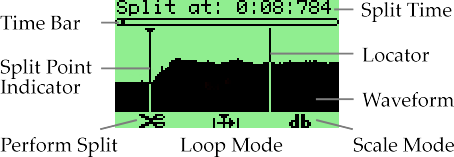
\includegraphics[width=8.0cm]{plugins/images/ss-splitedit-main-112x64x1}
      \caption{The Split Editor's Main Screen}
    \end{center}
  \end{figure}

\subsubsection{The Split Editor's Main Screen}
  \begin{description}
    \item[The waveform]
      displays the volume of the song over time. It will appear as the song
      plays and help to visually identify the point in time where the split is
      desired
      %
    \item[The split point indicator]
      is a vertical line with a small triangle at the top end. It is the most
      important control element of the split editor. It can be moved with the
      \ButtonLeft\ and \ButtonRight\ buttons. Later, when you have fine tuned
      the split point, the song will be split at this position.
      %
    \item[The split time]
      At the top of the window a time value is displayed. This is the point in
      time within the song at which the split point indicator is positioned.
      %
    \item[The locator]
      Another vertical bar represents the position locator. It moves along as
      the song plays. In contrast to the split point indicator it has no
      triangles at the ends.
      %
    \item[The time bar]
      displays the current position within the song relative to the whole song.
      The entire length of the time bar represents the song length. The length
      of the solid part of the time bar represents the position and length of
      the displayed part of the song.
      %
    \item[The scale mode]
      On the right side of the bottom line the scale mode is displayed. The
      waveform can be scaled either logarithmically or linearly. In logarithmic
      scale mode the letters ``dB'' are displayed, in linear mode ``\%''. Use
      \opt{RECORDER_PAD}{\ButtonFThree}
      \opt{ONDIO_PAD}{\ButtonMenu\ + \ButtonRight}
      to switch between these modes. Linear mode usually gives better optical
      hints with commercially recorded music. For quiet recordings,
      especially of human speech, the logarithmic scale often is preferable.
      More information in the Scale \reference{ref:Scalemode} below.
      %
    \item[The loop mode]
      In the middle of the bottom line the loop mode icon is displayed.
      There are 4 different loop modes. Pressing
      \opt{RECORDER_PAD}{\ButtonFTwo}
      \opt{ONDIO_PAD}{\ButtonMenu\ + \ButtonUp}
      changes to the next loop mode.
      %
      \begin{description}
        \item
        
\includegraphics[width=0.53cm]{plugins/images/icon-splitedit-loop-1}
          Playback loops around the split point indicator. This mode is best
          used when searching and zooming for the desired point at which to split
          the recording.
        \item
        
\includegraphics[width=0.53cm]{plugins/images/icon-splitedit-loop-2}
          Playback loops from the split point indicator to the end of the
          visible area. This mode is best used when fine tuning the split
          indicator position at the beginning of a recording.
        \item
        
\includegraphics[width=0.53cm]{plugins/images/icon-splitedit-loop-3}
          Playback loops from the beginning of the
          visible area to the split point. This mode is best used when fine
          tuning the split indicator position at the end of a recording.
        \item
        
\includegraphics[width=0.53cm]{plugins/images/icon-splitedit-loop-4}
          Playback does not loop, the borders of the visible
          area as well as the split point indicator are ignored. This mode is
          best used when playing the song outside of the borders of the displayed
          region.
      \end{description}
    \item[Perform the split (8)]
          The icon above the
          \opt{RECORDER_PAD}{\ButtonFOne}
          \opt{ONDIO_PAD}{\ButtonLeft}
          button indicates its function to execute the split. When split
          positioning is complete open the save dialogue with
          \opt{RECORDER_PAD}{\ButtonFOne}
          \opt{ONDIO_PAD}{\ButtonMenu\ + \ButtonLeft}.
  \end{description}

  \begin{table}
    \begin{btnmap}
      \ButtonOff & Quit plugin \\
      %
      \ButtonLeft\ / \ButtonRight &  Move the split point indicator \\
      %
      \ButtonUp\ / \ButtonDown & Zoom in / out \\
      %
      \opt{RECORDER_PAD}{\ButtonPlay}
      \opt{ONDIO_PAD}{\ButtonMenu}
      & Play from the split position \\
      %
      \opt{RECORDER_PAD}{\ButtonFOne}
      \opt{ONDIO_PAD}{\ButtonMenu\ + \ButtonLeft}
      & Enter the save dialogue \\
      %
      \opt{RECORDER_PAD}{\ButtonFTwo}
      \opt{ONDIO_PAD}{\ButtonMenu\ + \ButtonUp}
      & Toggle loop modes \\
      %
      \opt{RECORDER_PAD}{\ButtonFThree}
      \opt{ONDIO_PAD}{\ButtonMenu\ + \ButtonRight}
      & Toggle logarithmic / linear scaling \\
      \opt{RECORDER_PAD}{
      %
      \ButtonOn\ + \ButtonLeft
      & Play half speed \\
      %
      \ButtonOn\ + \ButtonRight
      & Play 150\% speed \\
      %
      \ButtonOn\ + \ButtonPlay
      & Play normal speed \\
    }
    \end{btnmap}
	\caption{Controls in the split editor}
  \end{table}

\subsubsection{Save dialogue}
In the save dialogue it is possible to specify which of the files you
want to save and their names.  When finished, select
``Save'' and the files will be written to
disk. Note that files can not be overwritten, so filenames that
do not exist yet must be chosen. If unsure whether the
file already exists simply try to save it. If another file with this
name exists the dialogue will return and you can choose another
filename

\screenshot{plugins/images/ss-splitedit-save}{The Split Editor's
Save Dialogue}{}

\begin{table}
  \begin{btnmap}
    \ButtonUp\ / \ButtonDown & Select item \\
    %
    \opt{RECORDER_PAD}{\ButtonPlay}
    \opt{ONDIO_PAD}{\ButtonRight}
    & Toggle / edit item \\
    %
    \ButtonOff & Cancel \\
  \end{btnmap}
  \caption{Controls in the save dialogue}
\end{table}

\subsubsection{\label{ref:Scalemode}Scale}
The values in the waveform are scaled according to the settings of the
peak meter. These can be altered in the peak meter settings,
see \reference{ref:Peakmetersetting}. If extreme minimum or
maximum values are set the waveform might be cut off.  A minimum
setting of {}-60~dB and a maximum setting of 0~dB are recommended.
These settings should be capable of producing useful waveforms for very
soft sounds in logarithmic mode (dB). When the editor is used on loud
sounds (such as commercial rock or pop music) switching to the linear
scale may prove more effective since the logarithmic scale compresses
loud noises and makes it more difficult to identify characteristic
shapes. Note that it is always possible to toggle between the two scale
modes.


}

{\subsection{Stats}
\screenshot{plugins/images/ss-stats}{The stats-plugin}{}

The stats plugin counts the directories and files%
\nopt{archosplayer}{ (the total number as well as the number
of audio, playlist, image and video files) }%
on your \dap{}.
Press \PluginCancel{} or \PluginExit{} to abort counting and
exit the plugin. Press it again to quit after counting has
finished.
}

{\subsection{Stopwatch}
\screenshot{plugins/images/ss-stopwatch}{Stopwatch}{fig:stopwatch}

A simple stopwatch program with support for saving times.

\begin{btnmap}
    \opt{PLAYER_PAD}{\ButtonMenu}
    \opt{RECORDER_PAD,ONDIO_PAD,IRIVER_H100_PAD,IRIVER_H300_PAD}{\ButtonOff}
    \opt{IPOD_4G_PAD,IPOD_3G_PAD}{\ButtonMenu}
    \opt{IAUDIO_X5_PAD,IRIVER_H10_PAD,SANSA_E200_PAD,SANSA_C200_PAD,GIGABEAT_PAD%
        ,MROBE100_PAD,SANSA_CLIP_PAD}{\ButtonPower}
    \opt{SANSA_FUZE_PAD}{Long \ButtonHome}
    \opt{GIGABEAT_S_PAD}{\ButtonBack}
    \opt{PBELL_VIBE500_PAD,SAMSUNG_YH92X_PAD,SAMSUNG_YH820_PAD}{\ButtonRec}
    \opt{MPIO_HD200_PAD}{\ButtonRec + \ButtonPlay}
    \opt{MPIO_HD300_PAD}{Long \ButtonMenu}
       \opt{HAVEREMOTEKEYMAP}{& 
          \opt{IRIVER_RC_H100_PAD}{\ButtonRCStop}
        }
    & Quit Plugin \\
    %
    \opt{PLAYER_PAD,RECORDER_PAD,IAUDIO_X5_PAD,IRIVER_H10_PAD,GIGABEAT_S_PAD%
        ,PBELL_VIBE500_PAD,MPIO_HD200_PAD,MPIO_HD300_PAD,SAMSUNG_YH92X_PAD%
        ,SAMSUNG_YH820_PAD}{\ButtonPlay}
    \opt{ONDIO_PAD,SANSA_E200_PAD,SANSA_FUZE_PAD,SANSA_C200_PAD%
        ,SANSA_CLIP_PAD}{\ButtonRight}
    \opt{IRIVER_H100_PAD,IRIVER_H300_PAD,GIGABEAT_PAD,MROBE100_PAD,IPOD_4G_PAD%
        ,IPOD_3G_PAD}{\ButtonSelect}
  \opt{HAVEREMOTEKEYMAP}{& }
    & Start / stop \\
    %
    \opt{PLAYER_PAD}{\ButtonStop}
    \opt{RECORDER_PAD,ONDIO_PAD,IPOD_4G_PAD,IPOD_3G_PAD,SANSA_E200_PAD%
        ,SANSA_FUZE_PAD,SANSA_C200_PAD,SANSA_CLIP_PAD,SAMSUNG_YH92X_PAD%
        ,SAMSUNG_YH820_PAD}{\ButtonLeft}
    \opt{IRIVER_H100_PAD,IRIVER_H300_PAD}{\ButtonDown}
    \opt{IRIVER_H10_PAD,MPIO_HD200_PAD,MPIO_HD300_PAD}{\ButtonRew}
    \opt{IAUDIO_X5_PAD}{\ButtonRec}
    \opt{GIGABEAT_PAD}{\ButtonA}
    \opt{GIGABEAT_S_PAD}{\ButtonMenu}
    \opt{MROBE100_PAD}{\ButtonDisplay}
    \opt{PBELL_VIBE500_PAD}{\ButtonOK}
  \opt{HAVEREMOTEKEYMAP}{& }
    & Reset timer (only when timer is stopped)\\
    %
    \opt{PLAYER_PAD,RECORDER_PAD,IRIVER_H100_PAD,IRIVER_H300_PAD}{\ButtonOn}
    \opt{ONDIO_PAD,GIGABEAT_PAD,MROBE100_PAD,PBELL_VIBE500_PAD}{\ButtonMenu}
    \opt{IPOD_4G_PAD,IPOD_3G_PAD,SAMSUNG_YH92X_PAD,SAMSUNG_YH820_PAD}{\ButtonRight}
    \opt{IRIVER_H10_PAD,MPIO_HD200_PAD,MPIO_HD300_PAD}{\ButtonFF}
    \opt{IAUDIO_X5_PAD,SANSA_E200_PAD,SANSA_FUZE_PAD,SANSA_C200_PAD,GIGABEAT_S_PAD%
        ,SANSA_CLIP_PAD}{\ButtonSelect}
  \opt{HAVEREMOTEKEYMAP}{& }
    & Take lap time \\
    %
    \opt{PLAYER_PAD,IRIVER_H100_PAD,IRIVER_H300_PAD}{\ButtonLeft{} / \ButtonRight}
    \opt{RECORDER_PAD,ONDIO_PAD,IAUDIO_X5_PAD,SANSA_E200_PAD,SANSA_FUZE_PAD%
        ,SANSA_C200_PAD,GIGABEAT_PAD,GIGABEAT_S_PAD,MROBE100_PAD,PBELL_VIBE500_PAD%
        ,SANSA_CLIP_PAD,SAMSUNG_YH92X_PAD,SAMSUNG_YH820_PAD}{\ButtonUp{} / \ButtonDown}
    \opt{IPOD_4G_PAD,IPOD_3G_PAD}{\ButtonScrollFwd{} / \ButtonScrollBack}
    \opt{IRIVER_H10_PAD,MPIO_HD300_PAD}{\ButtonScrollUp{} / \ButtonScrollDown}
    \opt{MPIO_HD200_PAD}{\ButtonVolUp / \ButtonVolDown}
  \opt{HAVEREMOTEKEYMAP}{& }
    & Scroll through lap times \\
\end{btnmap}
}

\opt{lcd_bitmap}{\subsection{\label{sec:text_editor}Text Editor}
This plugin allows you to view and edit simple text documents on your DAP.
You can view files by using \setting{Open with} from the
\setting{Context Menu} (see \reference{ref:Contextmenu}).

\subsubsection{Usage}
If you start the Text Editor from the plugin browser you will be greeted with
a blank screen. When started from the \setting{Open with} menu item your file 
should be shown on the screen. You can now edit the file.
The Text Editor is line based. This means you can edit one line at a time using
the \setting{Virtual Keyboard} (see \reference{sec:virtual_keyboard}).

\begin{itemize}
  \item Move the selection bar to the line you want to edit.
  \item Edit the highlighted text line or insert a new one using the Item Menu.
  \item When finished editing exit the Text Editor. You'll be shown a list of
        save options. 
\end{itemize}
\note{When you have not changed the file the Text Editor will quit immediately.}

\begin{btnmap}
    \ActionStdOk 
      \opt{HAVEREMOTEKEYMAP}{& \ActionRCStdOk}
    & Edit Line / Select Character\\

    \ActionStdCancel 
      \opt{HAVEREMOTEKEYMAP}{& \ActionRCStdCancel} 
    & Exit / Abort Editing\\

    \ActionStdMenu 
      \opt{HAVEREMOTEKEYMAP}{& \ActionRCStdMenu} 
    & Show Item Menu\\

    \ActionStdContext 
      \opt{HAVEREMOTEKEYMAP}{& \ActionRCStdContext} 
    & Delete Line\\
\end{btnmap}

}
